\documentclass[letterpaper,12pt]{report} 

\usepackage[spanish]{babel}
\usepackage[utf8]{inputenc}
\usepackage{graphicx}
\usepackage{amsfonts,amsmath,color,amssymb,float, amsthm}  
\usepackage{hyperref}
\usepackage[right=3cm,left=2cm,top=2cm,bottom=2cm,headsep=0.7cm,footskip=0.5cm]{geometry}
\usepackage{enumerate}
\usepackage{wrapfig} 
\usepackage[rflt]{floatflt}
\usepackage{xcolor} 
\usepackage{esint}
\usepackage{cancel}
\usepackage{listings}
\usepackage{pstricks, caption}
\providecommand{\norm}[1]{\lVert#1\rVert}
\providecommand{\Arg}[1]{Arg(#1)}

\decimalpoint

\newtheorem{teorema}{Teorema}[chapter] 
\newtheorem{ejemplo}{Ejemplo}[chapter] 
\newtheorem{defi}{Definici\'on}[chapter] 
\newtheorem{corolario}{Corolario}[chapter] 
\newtheorem{propo}{Proposición}[chapter] 
\newtheorem{lema}{Lema}[chapter] 
\newcommand{\grad}{^{\circ}}

\newlength{\drop}

%%%%%%%%%%%%Fancy Chapters%%%%%%%%%%%%%%%%%
%Options: Sonny, Lenny, Glenn, Conny, Rejne, Bjarne, Bjornstrup
\usepackage[Lenny]{fncychap}
%%%%%%%%%%%%%%%%%%%%%%%%%%%%%%%%%%%%%%%%%%%

\begin{document}
\begin{titlepage}
 \drop=0.1\textheight
    \centering
    \vspace*{\baselineskip}
    \rule{\textwidth}{1.6pt}\vspace*{-\baselineskip}\vspace*{2pt}
    \rule{\textwidth}{0.4pt}\\[\baselineskip]
    {\scshape\Huge Cálculo IV} \\[0.2\baselineskip]
    \rule{\textwidth}{0.4pt}\vspace*{-\baselineskip}\vspace{3.2pt}
    \rule{\textwidth}{1.6pt}\\[\baselineskip]
    {\Large Autor: \par}
{\Large Alejandro Saavedra \par}
\vfill
{\large Agosto 2022 \par}
{\large v1.0 \par}
\end{titlepage}
\tableofcontents

\chapter{Campo de los números complejos}

\section{Definiciones y propiedades algebraicas}

\begin{defi}
El \textbf{sistema de los números complejos}, denotado por $\mathbb{C}$, es el conjunto $\mathbb{R}^2$ junto con las operaciones:

\begin{enumerate}
\item de adición
\begin{equation}
(x_1, y_1) + (x_2,y_2) = (x_1 + y_1, x_2 + y_2) \label{Suma}
\end{equation}

\item y de multiplicación compleja siguiente:
\begin{equation}
(x_1, y_1) (x_2,y_2) = (x_1 x_2 - y_1y_2, x_1 y_2 + y_1x_2). \label{Multiplicacion}
\end{equation}

\end{enumerate}

Los elementos $z = (x,y)$ de $\mathbb{C}$ se llaman \textbf{números complejos}, donde $x$ es la \textbf{parte real} de $z$ e $y$ la \textbf{parte imaginaria}. Lo anterior se denota por
$$Re(z) = x ~~\mbox{e}~~ Im(z) = y.$$

Diremos que un complejo es \textbf{imaginario puro} si $z = (0,y)$. En particular, al número $(0,1)$ lo denotaremos por $i$.
\end{defi}

\textbf{Observación:} Cada número real $x$ puede ser identificado como el complejo $z = (x,0)$; de esta manera, asumiremos siempre que $\mathbb{R} \subset \mathbb{C}$. Notar que si $z_1 = (x_1,0)$ y $z_2 = (x_2,0)$, entonces
\begin{eqnarray*}
z_1 + z_2 &=& (x_1 + x_2, 0), \\
z_1z_2 &=& (x_1x_2, 0),
\end{eqnarray*}

es decir, que las operaciones \eqref{Suma} y \eqref{Multiplicacion} coinciden con las operaciones en $\mathbb{R}$. Más aún, si $(\alpha,0) \in \mathbb{R}$ y $z = (x,y)$ es cualquier otro complejo, se tiene
$$(\alpha,0)z = (\alpha x, \alpha y),$$

es decir, tenemos la operación multiplicación por escalar en $\mathbb{R}^2$.

\begin{defi}
Diremos que dos complejos $z_1 = (x_1,y_1)$ y $z_2 = (x_2, y_2)$ son iguales si y sólo si
$$x_1 = x_2 ~\wedge~ y_1 = y_2.$$
\end{defi}

En lugar de usar $(x,y)$  para representar a los números complejos, encontraremos otra forma más conveniente y natural de identificarlos. 
Si $z = (x,y) \in \mathbb{C}$, entonces
\begin{eqnarray*}
z &=& (x,y) \\
&=& (x,0) + (0,y) \\
&=& (x,0) + (y,0) (0,1) \\
&=& x + yi = x+iy.
\end{eqnarray*}

Esta forma de denotar a los números complejos es conocida como \textbf{forma binómica} de $z$.

\begin{teorema}
El conjunto $\mathbb{C}$ con las operaciones \eqref{Suma} y \eqref{Multiplicacion} resulta ser un cuerpo conmutativo.
\end{teorema}

\begin{proof}
Sean $z_1 = (x_1,y_1)$, $z_2 = (x_2,y_2)$ y $z_3 = (x_3, y_3)$ números complejos cualesquiera. Probaremos los 9 axiomas de los cuerpos conmutativos, teniendo en cuenta que $\mathbb{R}$ es un cuerpo. 

\begin{enumerate}
\item La suma es conmutativa. En efecto,
$$z_1 + z_2 = (x_1 + x_2, y_1 + y_2) = (x_2 + x_1, y_2 + y_1) = z_2 + z_1.$$

\item La suma es asociativa. En efecto,
\begin{eqnarray*}
z_1 + (z_2 + z_3) &=& (x_1,y_1) + ((x_2,y_2) + (x_3,y_3)) \\
&=& (x_1 ,y_1) + (x_2 + x_3, y_2 + y_3 )  \\
&=& (x_1 + (x_2 + x_3), y_1 + (y_2 + y_3)) \\
&=& ((x_1 + x_2) + x_3, (y_1 + y_2) + y_3) \\
&=& (x_1 + x_2, y_1 + y_2)  + z_3 \\
&=& (z_1 + z_2) + z_3.
\end{eqnarray*}

\item Existe un elemento neutro para la suma. En efecto, si consideramos el complejo $(0,0)$, se tiene
$$z_1 + (0,0) = (x_1,y_1) + (0,0) = (x_1, y_1) = z_1.$$

\item Cada $z_1$ tiene un inverso para la suma. En efecto, si consideramos el complejo $(-x_1, -y_1)$, se verifica
$$z_1 + (-x_1, -y_1) = (x_1 + (-x_1), y_1 + (-y_1)) = (0,0).$$

\item El producto es conmutativo. En efecto, 
$$z_1 z_2 = (x_1, y_1) (x_2,y_2) = (x_1 x_2 - y_1y_2, x_1 y_2 + y_1x_2) = (x_2 x_1 - y_2y_1,  x_2y_1 + y_2x_1 ) = z_2 z_1.$$

\item El producto es asociativo. En efecto,
\begin{eqnarray*}
z_1 (z_2 z_3) &=& (x_1,y_1) (x_2x_3 - y_2y_3, x_2y_3 + y_2 x_3) \\
&=& (x_1(x_2 x_3 - y_2y_3) - y_1 (x_2y_3 + y_2 x_3), x_1 (x_2y_3 + y_2x_3) + y_1(x_2x_3 - y_2y_3)) \\
&=& ((x_1x_2 - y_1y_2)x_3 - (x_1 y_2 + y_1x_2)y_3 , (x_1 x_2 - y_1y_2) y_3 + (x_1 y_2 + y_1 x_2)x_3) \\
&=& (x_1 x_2 - y_1y_2, x_1y_2 + y_1 x_2)(x_3,y_3) \\
&=& (z_1 z_2) z_3.
\end{eqnarray*}

\item Existe un elemento neutro para el producto. En efecto, si consideramos el complejo $(1,0)$, se tiene
$$z_1 (1,0) = (x_1 - 0, 0 + y_1) = (x_1,y_1) = z_1.$$

\item Cada $z_1 \neq (0,0)$ tiene un inverso para el producto. En efecto, supongamos que existe $w = (w_x, w_y) \in \mathbb{C} \setminus \{(0,0)\}$ tal que
$$z_1 w = (1,0) ~\Leftrightarrow~(x_1 w_x - y_1 w_y, x_1w_y + y_1 w_x) = (1,0).$$

Por igualdad de los números complejos:
\begin{equation*}
 \left\{ \begin{array}{ccl}
x_1 w_x - y_1 w_y &=& 1 \\
y_1 w_x + x_1 w_y &=& 0
\end{array}  \right.  ~\Leftrightarrow~ \left\{ \begin{array}{ccl}
 w_x  &=& \frac{x_1}{x_1^2 + y_1^2} \\
 w_y &=& - \frac{y_1}{x_1^2 + y_1^2}
\end{array}  \right.  .
\end{equation*}

Como $z_1 \neq (0,0)$, $w$ está bien definido y por las equivalencias hemos probado que existe el inverso multiplicativo.

\item El producto es distributivo con respecto a la suma. En efecto,
\begin{eqnarray*}
z_1 (z_2 + z_3) &=& (x_1, y_1) (x_2 + x_3, y_2 + y_3) \\
&=& (x_1 (x_2 + x_3) - y_1(y_2 + y_3), x_1 (y_2 + y_3) + y_1(x_2 + x_3)) \\
&=& ((x_1x_2 - y_1 y_2) + (x_1x_3 - y_1y_3), (x_1 y_2 + y_1 x_2) + (x_1 y_3 + y_1 x_3)) \\
&=& (x_1 x_2 - y_1 y_2, x_1 y_2 + y_1x_2) + (x_1 x_3 - y_1y_3, x_1 y_3 + y_1 x_3) \\
&=& z_1 z_2 + z_1 z_3.
\end{eqnarray*}
\end{enumerate}

\end{proof}

\textbf{Nota:} 

\begin{itemize}
\item[(i)] Identificaremos a los complejos $(0,0)$ y $(1,0)$ por $0$ y $1$, respectivamente.

\item[(ii)] Denotaremos al inverso aditivo del complejo $z$ por $-z$.

\item[(iii)] Denotaremos al inverso multiplicativo del complejo $z = (x,y)$ por $z^{-1}$. Luego,
$$z^{-1} = \left( \frac{x}{x^2 + y^2}, - \frac{y}{x^2+y^2} \right) = \frac{x}{x^2 + y^2} + i \frac{-y}{x^2+y^2}.$$

\item[(iv)] Las potencias de números complejos se definen de forma inductiva como: $z^2 = zz, z^3 = zz^2, \dots, z^n = z z^{n-1}$. Notar que $i^2 = -1$; $i^3 = -i$; $i^4 = 1$. Entonces, el subconjunto $\{1, i,i^2, i^3\}$ forma un subgrupo del grupo $(\mathbb{C}, \cdot)$ con la siguiente tabla de Cayley: \footnote{Un \textit{grupo} es un conjunto $G$ con una operación binaria $\cdot: G \times G \rightarrow G$ tal que es cerrada, asociativa, existe una identidad y un inverso. Todos los productos posibles entre los elementos del grupo pueden ser representados en una tabla conocida como \textit{tabla de Cayley}. Un \textit{subgrupo} de un grupo $G$ es una subconjunto de $G$ que es a su vez un grupo.}
\begin{equation*}
\left[ \begin{array}{c|cccc}
\cdot & 1 & i & i^2 & i^3 \\
\hline
1 & 1 & i & i^2 & i^3 \\
i & i & i^2 & i^3 & 1 \\
i^2 & i^2 & i^3 & 1 & i \\
i^3 & i^3 & 1 & i & i^2
\end{array} \right] .
\end{equation*}
\end{itemize}

\newpage

\begin{defi}
Sean $z_1, z_2 \in \mathbb{C}$, definimos:

\begin{itemize}
\item la \textbf{diferencia} entre $z_1$ y $z_2$ por
$$z_1 - z_2 := z_1 + (-z_2),$$

\item el \textbf{cociente}  entre $z_1$ y $z_2$ por
$$\frac{z_1}{z_2} := z_1 z_2^{-1}, \quad z_2 \neq 0.$$

\end{itemize}
\end{defi}

\textbf{Observación:}  Si $z_1 = (x_1,y_1)$ y $z_2 = (x_2, y_2)$, entonces
\begin{equation*}
\frac{z_1}{z_2} = \left( \frac{x_1x_2 + y_1y_2}{x_2^2 + y_2^2}, \frac{x_2 y_1 - x_1y_2}{x_2^2 + y_2^2} \right) = \frac{x_1x_2 + y_1y_2}{x_2^2 + y_2^2} + i \frac{x_2 y_1 - x_1y_2}{x_2^2 + y_2^2}.
\end{equation*}

\begin{propo}
Sean $z_1, z_2 \in \mathbb{C}$ tales que
$$z_1 z_2 = 0 ~\Rightarrow~ z_1 = 0 ~\vee~ z_2 = 0.$$
\end{propo}

\begin{proof}

Existen dos posibilidades, que $z_1 =0$ o que $z_1 \neq 0$.

Si $z_1 = 0$, la disyunción de la tesis es verdadera.

Si $z_1 \neq 0$, entonces $\exists z_1^{-1}$ tal que $z_1 z_1^{-1} = 1$. Así,
\begin{eqnarray*}
z_1 z_2 &=& 0 \quad \color{red}{/ \cdot z_1^{-1}}\\
\Rightarrow \, (z_1 z_2) z_1^{-1} &=& 0 \cdot z_1^{-1} \\
\Rightarrow \, (z_1  z_1^{-1}) z_2 &=& 0 \\
\Rightarrow \qquad \quad ~ \,z_2 &=& 0.
\end{eqnarray*}

Luego, en ambos casos se verifica la tesis.

\end{proof}

\textbf{Observación:} Finalmente, remarcamos que el orden usual de los números reales no puede ser extendido a los complejos. Así, $z_1 < z_2$ tiene sentido si y sólo si, $z_1, z_2 \in \mathbb{R}$. Esta afirmación puede ser probada de la siguiente  manera: supóngase que tal orden existe, entonces o $i \geq 0$, o $i \leq 0$. Supongamos que $i \geq 0$, entonces $i \cdot i \geq 0$ y, por lo tanto, $-1 \geq 0$, lo cual es absurdo. Alternativamente, si suponemos $i \leq 0$, entonces $-i \geq 0$, así $(-i)(-i) \geq 0$ o $-1 \geq 0$, otra vez absurdo. 

\begin{teorema}[del Binomio de Newton]
Sean $z, w \in \mathbb{C}$ y $n \in \mathbb{N}$, se tiene la siguiente igualdad
$$(z+w)^n = \sum_{k=0}^n {n \choose k} z^{n-k}w^k$$

donde $${n \choose k} = \frac{n!}{(n-k)! k!}.$$
\end{teorema}

\begin{proof}
Usando inducción de la misma forma que en el caso real.
\end{proof}

\begin{defi}
El \textbf{módulo} de un complejo $z = x+iy$ está definido por
$$|z| := \sqrt{x^2 + y^2}.$$
\end{defi}

\textbf{Representación gráfica:} Como $\mathbb{C}$ es $\mathbb{R}^2$ con las operaciones definidas anteriormente, podemos identificar cada número complejo $z = x + iy$ con el punto $(x,y)$ en el plano cartesiano. El plano $xy$ se llama \textbf{plano complejo}. El eje $x$ se llama \textbf{eje real} y el eje $y$ se llama \textbf{eje imaginario}. 

El módulo $|z|$, geométricamente, corresponde a la distancia entre el origen y el punto $(x,y)$ en el plano complejo.

La figura \ref{SumaComplejos} ilustra la interpretación geométrica de la suma y la resta entre números complejos.

\begin{figure}[H]
    \centering
    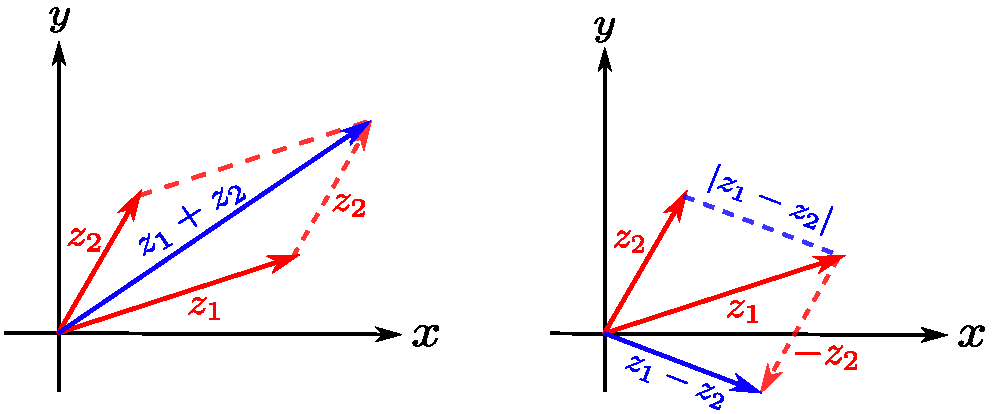
\includegraphics[scale=0.7]{Figuras/SumaCompejos.pdf}
    \caption{Interpretación geométrica de la suma y resta de números complejos.}
    \label{SumaComplejos}
\end{figure}

\begin{defi}
Para $z = x+iy \in \mathbb{C} $, definimos el \textbf{conjugado} de $z$ por el número
$$\bar{z} := x -iy.$$
\end{defi}

\textbf{Observación:} Geométricamente, $\bar{z}$ es la reflexión con respecto al eje $x$ del complejo $z$.

\begin{figure}[H]
    \centering
    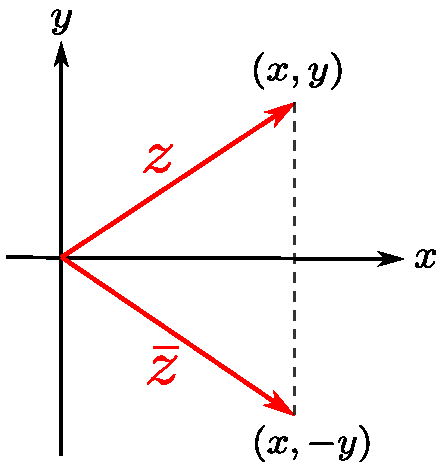
\includegraphics[scale=0.6]{Figuras/Conjugado.pdf}
    \caption{Gráfica del complejo conjugado.}
    \label{ComplejoConjugado}
\end{figure}

\begin{propo}\label{PropiedadesConjugadoModulo}
Si $z,z_1,z_2 \in \mathbb{C}$, entonces:

\begin{enumerate}
\item $$\overline{z_1 + z_2} = \overline{z_1} + \overline{z_2}; \quad \overline{z_1z_2} = \overline{z_1} \, \overline{z_2}; \quad \overline{\frac{z_1}{z_2}} = \frac{\overline{z_1}}{\overline{z_2}}, ~~ z_2 \neq 0.$$

\item $$z + \bar{z} \in \mathbb{R}; \quad \bar{\bar{z}} = z; \quad Re(z) = \frac{z + \bar{z}}{2};\quad Im(z)= \frac{z - \bar{z}}{2i}.$$

\item $$z \bar{z} = |z|^2; \quad |z| = |\bar{z}|; \quad \max\{|Re(z)|, |Im(z)|\} \leq |z|.$$

\item $$|z_1 z_2| = |z_1| \, |z_2|; \quad \left| \frac{z_1}{z_2} \right| = \frac{|z_1|}{|z_2|}, ~~ z_2 \neq 0.$$
\end{enumerate}

\end{propo}

\begin{proof}
Sean $z = x+iy$, $z_1 = x_1 + iy_1$ y $z_2 = x_2 + iy_2$ números complejos cualesquiera.

\begin{enumerate}
\item \begin{eqnarray*}
\overline{z_1 + z_2}  &=& \overline{(x_1+x_2) + i(y_1 + y_2)} \\\
&=&(x_1+x_2) - i(y_1 + y_2) \\
& =& (x_1 - iy_1) + (x_2 - iy_2) = \overline{z_1} + \overline{z_2}. \\
\overline{z_1 z_2} &=&  \overline{(x_1 x_2 - y_1y_2) + i(x_1y_2 + y_1x_2)} \\
&=&  (x_1 x_2 - y_1y_2) - i(x_1y_2 + y_1x_2) \\
&=& (x_1 -iy_1) (x_2 - iy_2) = \overline{z_1} \, \overline{z_2}.  \\
\overline{\frac{z_1}{z_2}} &=& \overline{z_1 z_2^{-1}} \\
&=& \overline{z_1} \, \overline{z_2^{-1}} \\
&=& \overline{z_1} \, \frac{x_2 - i(-y_2)}{x_2^2 + y_2^2} \\
&=& \overline{z_1} \, (\overline{z_2})^{-1} = \frac{\overline{z_1}}{\overline{z_2}}, ~~ z_2 \neq 0.
\end{eqnarray*}

\item \begin{eqnarray*}
z + \bar{z} &=& (x+iy) + (x-iy) = 2x \in \mathbb{R}. \\
\bar{\bar{z}} &=& \overline{x -iy} = x+iy = z. \\
Re(z) &=& \frac{(x+iy) + (x-iy)}{2} = \frac{z + \bar{z}}{2}. \\
Im(z) &=& \frac{(x+iy) - (x-iy)}{2i} = \frac{z - \bar{z}}{2i}.
\end{eqnarray*}

\item \begin{eqnarray*}
z \bar{z} &=& (x+iy)(x-iy) = x^2 + y^2 = |z|^2. \\
|z| &=& \sqrt{x^2+y^2} = \sqrt{x^2 + (-y_2)^2} = |\bar{z}|.
\end{eqnarray*}

Del cálculo III, sabemos que
$$|x| \leq \norm{(x,y)} ~~\mbox{y}~~ |y| \leq \norm{(x,y)}.$$

Como $Re(z) = x$ e $Im(z) = y$, se tiene que
$$\max\{|Re(z)|, |Im(z)|\} \leq \sqrt{x^2+y^2} = |z|.$$

\item 
\begin{equation*}
|z_1 z_2|^2 = (z_1 z_2) \, (\overline{z_1z_2}) = (z_1 \overline{z_1}) (z_2 \overline{z_2}) = |z_1|^2|z_2|^2 = (|z_1||z_2|)^2 ~\Rightarrow~ |z_1 z_2| = |z_1||z_2|.
\end{equation*}
\begin{equation*}
\left| \frac{z_1}{z_2} \right| = \left|z_1 z_2^{-1}\right| = |z_1| \, |z_2^{-1}| = |z_1| \, \left| \frac{x-iy}{x^2+y^2} \right| = |z_1| \, \frac{\sqrt{x^2+y^2}}{x^2+y^2} = |z_1| \,|z_2|^{-1} = \frac{|z_1|}{|z_2|}.
\end{equation*}

\end{enumerate}
\end{proof}

\begin{propo}[Desigualdad triangular]
Para cualquier par de números complejos $z_1$ y $z_2$, se tiene
$$|z_1 + z_2| \leq |z_1| + |z_2|.$$
\end{propo}

\begin{proof}
Utilizando las propiedades dadas en la proposición \ref{PropiedadesConjugadoModulo}, se tiene que
\begin{eqnarray*}
|z_1 + z_2|^2 &=& (z_1 + z_2) \overline{(z_1 + z_2)} \\
&=& (z_1 + z_2)(\overline{z_1} + \overline{z_2}) \\
&=& z_1 \overline{z_1} + z_1 \overline{z_2} + z_2 \overline{z_1} + z_2 \overline{z_2} \\
&=& |z_1|^2 + (z_1 \overline{z_2} + \overline{z_1 \overline{z_2}}) + |z_2|^2.
\end{eqnarray*}

Ahora, como $z_1 \overline{z_2} + \overline{z_1 \overline{z_2}}= 2 Re(z_1 \overline{z_2}) \leq 2 |z_1 \overline{z_2}| = 2 |z_1| \; |z_2|$, obtenemos que
$$|z_1 + z_2|^2 \leq |z_1|^2 + 2  |z_1| \; |z_2| + |z_2|^2 = (|z_1| + |z_2|)^2.$$

Por lo tanto,
$$|z_1 + z_2| \leq |z_1| + |z_2|.$$
\end{proof}

Por inducción, se puede demostrar que
\begin{corolario}
Si $z_1, z_2, \dots, z_n \in \mathbb{C}$, entonces
$$\left| \sum_{i=1}^n z_i \right| \leq \sum_{i=1}^n |z_i|.$$
\end{corolario}

\begin{corolario}
Si $z_1, z_2 \in \mathbb{C}$, entonces
$$||z_1| - |z_2|| \leq |z_1 + z_2|.$$
\end{corolario}

\begin{proof}
Sean $z_1, z_2 \in \mathbb{C}$ cualesquiera, se tiene que
\begin{equation}
|z_1| = |(z_1 + z_2) - z_2| \leq |z_1 + z_2| + |z_2| ~\Rightarrow~ |z_1| - |z_2| \leq |z_1 + z_2| \label{Desi.Trian1}
\end{equation}

y 
\begin{equation}
|z_2| = |(z_1 + z_2) - z_1| \leq |z_1 + z_2| + |z_1| ~\Rightarrow~ - |z_1 + z_2| \leq |z_1| - |z_2| \label{Desi.Trian2}.
\end{equation}

Combinando \eqref{Desi.Trian1} y \eqref{Desi.Trian2}, obtenemos
$$- |z_1 + z_2| \leq |z_1| - |z_2| \leq |z_1 + z_2| \Leftrightarrow ||z_1| - |z_2|| \leq |z_1 + z_2|.$$
\end{proof}

\section{Forma polar}

En coordenadas cartesianas, un complejo $z$ se identifica con un punto del plano de coordenadas $(x,y)$. Por otro lado, las coordenadas polares de este punto están dadas por las ecuaciones
\begin{eqnarray*}
x &=& r \cos \theta, \\
y &=& r \sin \theta .
\end{eqnarray*}

\begin{figure}[H]
    \centering
    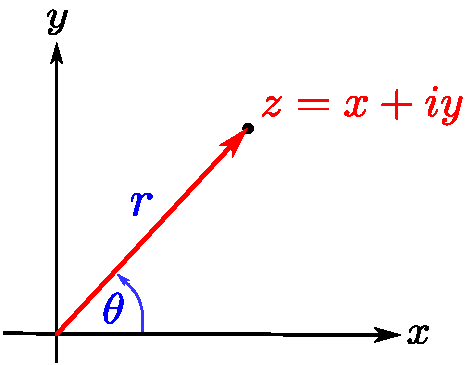
\includegraphics[scale=0.6]{Figuras/Polar.pdf}
    \caption{Coordenadas polares del complejo $z = x +iy$.}
    \label{Polares}
\end{figure}

donde $r$ es la longitud del segmento que une el origen con el punto $(x,y)$ y $\theta$ es la magnitud, en radianes, del ángulo que forma este segmento con la parte positiva del eje $x$.

Así,
$$z = x+iy = r \cos \theta + ir \sin \theta = r (\cos \theta + i \sin\theta).$$

A esta última expresión se le conoce como la \textbf{forma polar} del complejo $z$. 

El ángulo $\theta$ se llama \textbf{argumento} de $z$ y se denota por
$$\theta = \arg(z).$$

Notar que $r = |z|$ y que 
$$\tan \theta = \frac{y}{x}.$$

\textbf{Observación:} Si $z = 0$, $\theta$ está indefinido. De modo que cualquier número complejo que vaya ser escrito en polares se sobreentiende que es distinto de cero.

\begin{ejemplo}
 La forma polar del complejo $z = 1+i$ es
\begin{eqnarray*}
z &=& \sqrt{2} \left( \cos \frac{\pi}{4} + i \sin \frac{\pi}{4} \right) \\
&=& \sqrt{2} \left( \cos \left( -\frac{7\pi}{4}\right) + i \sin \left( - \frac{7\pi}{4} \right) \right).
\end{eqnarray*} 
\end{ejemplo}

De este ejemplo, se desprende que el $\arg(z)$ no es único.

En general, se tiene que
$$z = r [\cos (\theta + 2k\pi) + i \sin(\theta + 2k\pi)], \quad k \in \mathbb{Z},$$

donde $\theta$ es cualquier valor particular del argumento  de $z$.
\\

El \textbf{argumento principal} de $\arg(z)$, denotado $\Arg{z}$, se define como el único valor de $\arg(z)$ tal que $- \pi < \arg(z) \leq \pi$.

Luego, es conveniente definir el argumento de un número complejo como la función multievaluada
$$\arg(z) \equiv \Arg{z} + 2k \pi, \quad z \in \mathbb{Z},$$

es decir, $\arg(z)$ corresponde a un \underline{conjunto} de valores para un determinando $z \in \mathbb{C}$.
\\

En el caso del ejemplo anterior, el argumento principal de $1+i$ es $Arg(z) = \frac{\pi}{4}$.
\\

Ahora, si consideramos $z_1 = -1$ y $z_2 = i$, entonces $z_1 z_2 = -i$ y, en tal caso, tenemos
$$arg(z_1 z_2) = arg(-i) = \frac{3}{2}\pi = \pi + \frac{\pi}{2} = arg(z_1) + arg(z_2).$$

Pero,
$$Arg(z_1) = \pi; \quad Arg(z_2) = \frac{\pi}{2};\quad Arg(z_1z_2) = - \frac{\pi}{2}.$$

Lo que muestra que 
$$Arg(z_1z_2) \neq Arg(z_1) + Arg(z_2).$$

Sin embargo, para el argumento, se tiene la siguiente proposición.

\begin{propo}
Si $z_1, z_2 \in \mathbb{C}\setminus \{0\}$, entonces
\begin{equation}
arg(z_1z_2) = arg(z_1) + arg(z_2).\label{Producto.arg}
\end{equation}
\end{propo}

\begin{proof}
Supongamos que
\begin{equation}
z_1 = |z_1| [\cos ( \arg(z_1)) + i \sin( \arg(z_1))]; \quad z_2 = |z_2| [\cos( \arg(z_2)) + i \sin ( \arg(z_2))], \label{DosComplejos}
\end{equation}

donde 
\begin{align*}
    \arg(z_1) = \Arg{z_1} + 2 k_1 \pi = \theta_1 + 2 k_1 \pi  ; \quad k_1 \in \mathbb{Z}, \\
     \arg(z_2) = \Arg{z_2} + 2 k_2 \pi= \theta_2 + 2 k_2 \pi ; \quad k_2 \in \mathbb{Z}.
\end{align*}

Luego,
\begin{eqnarray*}
z_1 z_2 &=& |z_1| |z_2| [\cos ( \arg(z_1)) + i \sin( \arg(z_1))][\cos ( \arg(z_2)) + i \sin( \arg(z_2))] \\
&=& |z_1 z_2| (\cos \theta_1 + i \sin\theta_1)(\cos \theta_2 + i \sin \theta_2) \\
&=& |z_1 z_2| [(\cos \theta_1 \cos \theta_2 - \sin \theta_1 \sin\theta_2) + i(\sin\theta_1 \cos\theta_2 + \sin\theta_2 \cos \theta_1) ] \\
&=& |z_1 z_2| (\cos(\theta_1 + \theta_2) + i \sin(\theta_1 +  \theta_2)).
\end{eqnarray*}

Así,
$$\arg(z_1 z_2) = \theta_ 1 + \theta_2 + 2k_{12} \pi = \Arg{z_1} + \Arg{z_2} + 2k_{12} \pi, \quad k_{12} \in \mathbb{Z}.$$

Entonces, hemos establecido que 
\begin{align*}
    \arg(z_1) + \arg(z_2) &= \Arg{z_1} + \Arg{z_2} + 2 (k_1 + k_2)\pi, \\
    \arg(z_1 z_2) &= \Arg{z_1} + \Arg{z_2} + 2 k_{12}.
\end{align*}

Como $k_1$, $k_2$ y $k_{12}$ son enteros arbitrarios, $ \arg(z_1) + \arg(z_2)$ y $ \arg(z_1 z_2)$ coinciden como conjuntos.
\end{proof}

Geométricamente, el producto $z_1z_2$ en forma polar, se aprecia en la siguiente figura.

\begin{figure}[H]
    \centering
    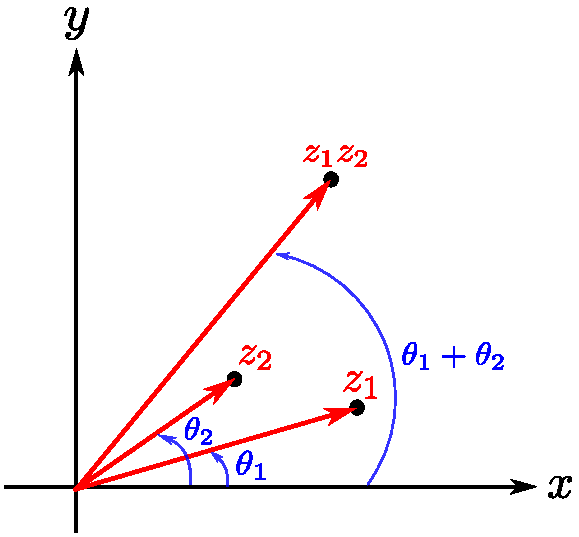
\includegraphics[scale=0.6]{Figuras/MultiplicacionComplejos.pdf}
    \caption{Interpretación geométrica del producto de números complejos en forma polar.}
    \label{ProductosComplejos}
\end{figure}

La ecuación 
$$z_1 z_2 = r_1r_2 (\cos(\theta_1 + \theta_2) + i \sin(\theta_1 +  \theta_2))$$

nos dice que la forma polar del único inverso multiplicativo de un número complejo no nulo
$$z = r (\cos \theta + i \sin \theta)$$

es
$$z^{-1} = \frac{1}{r} [\cos(-\theta) + i \sin(-\theta)],$$

siendo el producto de estas formas polares igual a la unidad.
\\

Como $\frac{z_1}{z_2} = z_1z_2^{-1}$, tenemos la siguiente expresión para el cociente de los dos números complejos no nulos \eqref{DosComplejos}:
$$\frac{z_1}{z_2} = \frac{r_1}{r_2} [\cos (\theta_1 - \theta_2) + i \sin(\theta_1- \theta_2)].$$

De la misma manera que el producto, ésto puede utilizarse para comprobar la afirmación
$$arg\left( \frac{z_1}{z_2} \right) = arg(z_1) - arg(z_2).$$
 
\section{Fórmula de Euler, potencias y raíces}

La ecuación
$$e^{i\theta} = \exp(i\theta) = \cos\theta + i \sin \theta$$

válida para todo $\theta \in \mathbb{R}$, se conoce como \textbf{fórmula de Euler}. 

Notemos que
$$e^{i \theta_1} e^{i \theta_2} = e^{i(\theta_1 + \theta_2)}$$

el cual corresponde al mismo tratamiento que conocemos del caso real. En particular,
$$e^{i\theta} e^{-i\theta} = 1,$$

es decir, $e^{- i\theta} = \frac{1}{e^{i\theta}}$ corresponde al inverso multiplicativo de $e^{i\theta}$.
\\

Si escribimos un número complejo no nulo en forma polar
$$z = r (\cos\theta + i \sin\theta),$$

la fórmula de Euler permite expresar $z$ más conveniente en \textbf{forma exponencial}:
$$z = r e^{i\theta}$$

y su inverso multiplicativo resulta ser
$$z^{-1} = \frac{1}{r} e^{-i\theta}.$$

Sean los complejos no nulos $z_1 = r_1 e^{i\theta_1}$ y $z_2 = r_2 e^{i\theta_2}$, se tiene que
\begin{eqnarray*}
z_1z_2 &=& r_1r_2 e^{i(\theta_1 + \theta_2)}. \\
\frac{z_1}{z_2} &=& \frac{r_1}{r_2} e^{i(\theta_1 - \theta_2)}.
\end{eqnarray*}

Es evidente que dos números complejos no nulos $z_1 = r_1 e^{i\theta_1}$ y $z_2 = r_2 e^{i\theta_2}$ son iguales si y sólo si $r_1 = r_2$ y $\theta_1 = \theta_2 + 2k\pi$, para algún $k \in \mathbb{Z}$.

\begin{teorema}
Sea $n \in \mathbb{Z}$ y sea $z= r (\cos \theta + i \sin \theta)$ un número complejo en forma polar. Entonces,
$$z^n = r^n (\cos (n\theta) + i\sin(n\theta)).$$
\end{teorema}

\begin{proof}
\
\\

\textbf{Caso 1:} Si $n > 0$, procederemos por inducción.

Para $n = 1$, es fácil de ver que el teorema se verifica.

Supongamos que para $n \in \mathbb{N}$ se satisface:
$$z^n = r^n (\cos(n\theta) + i \sin(n\theta).$$

Luego,
\begin{eqnarray*}
z^{n+1} = z^n z &=& [r^n (\cos (n\theta) + i\sin(n\theta))][r (\cos \theta + i \sin \theta)] \\
&=& r^{n+1} (\cos((n+1) \theta)) + i \sin((n+1) \theta))).
\end{eqnarray*}

Por lo tanto, el teorema es cierto para $n \in \mathbb{N}$.

\textbf{Caso 2:} Si $n = 0$, el convenio $z^0=1$ nos permite escribir: $z^0 = r^0 (\cos(0\cdot \theta) + i \sin(0 \cdot \theta)).$
\\

\textbf{Caso 3:} Si $n <0$, entonces
\begin{eqnarray*}
z^n = (z^{-1})^{-n} &=& r^n (\cos((-n)(-\theta)) + i \sin((-n)(-\theta))) \\
&=& r^n (\cos (n\theta) + i\sin(n\theta)).
\end{eqnarray*}

De esta manera, el teorema se verifica para todo $n \in \mathbb{Z}$.

\end{proof}

\textbf{Observación:} Equivalentemente, en forma exponencial, el teorema dice $(re^{i\theta})^n = r^n e^{in\theta}$. Si $r= 1$, obtenemos la \textbf{fórmula de De Moivre}:
$$(\cos \theta + i \sin\theta)^n = \cos(n \theta) + i \sin(n\theta).$$

\begin{defi}
Sea $n \in \mathbb{N}$. Dado un número complejo $z_0$, decimos que $z$ es una raíz $n$-ésima de $z_0$ si $z^n = z_0$.
\end{defi}

\begin{teorema}
Si $n \in \mathbb{N}$ y $z_0 \in \mathbb{C} \setminus \{0\}$ con forma polar $z_0 = r_0 (\cos \theta_0 + i \sin\theta_0) $, entonces $z_0$ tiene exactamente $n$ raíces $n$-ésimas distintas dadas por
$$\sqrt[n]{r_0} \left[ \cos \left( \frac{\theta_0 + 2k\pi}{n} \right) + i \sin \left( \frac{\theta_0 + 2k\pi}{n} \right)\right], \quad k = 0,1, \dots, n-1.$$
\end{teorema}

\begin{proof}
Las raíces $n$-ésimas de $z_0$ son los $z \in \mathbb{C}$ tales que
$$z^n = z_0.$$

Ésto implica que
$$|z^n| = |z|^n = |z_0|~\Rightarrow~ |z| = \sqrt[n]{|z_0|} = \sqrt[n]{r_0}.$$

Escribiendo $z$ en forma polar, $z = r (\cos \theta + i \sin \theta)$, obtenemos:
\begin{eqnarray}
[r (\cos \theta + i \sin \theta)]^n &=& r_0 (\cos \theta_0 + i \sin\theta_0)  \\
\Leftrightarrow ~ r^n (\cos (n\theta) + i \sin (n\theta)) &=& r_0 (\cos \theta_0 + i \sin\theta_0) \\
\Leftrightarrow \quad r^n \cos(n\theta) = r_0 \cos\theta_0  &\wedge & r^n \sin (n\theta)  = r_0 \sin \theta_0. \label{raíz}
\end{eqnarray}

Como $|z| = r = \sqrt[n]{r_0}$, la ecuación \eqref{raíz} nos queda
\begin{eqnarray}
\cos(n\theta) = \cos\theta_0  &\wedge &   \sin (n\theta)  =  \sin \theta_0 \\
\Rightarrow \qquad \qquad \qquad n \theta &=& \theta_0 + 2 m\pi, \quad m \in \mathbb{Z} \\
\Rightarrow  \qquad \qquad \qquad ~~ \theta &=& \frac{\theta_0}{n} + \frac{2 m \pi}{n}, \quad m \in \mathbb{Z}. \label{raiz2}
\end{eqnarray}

Ahora, por el algoritmo de la división, la división de los enteros $m/n$ nos dice que existen $q \in \mathbb{Z}$ (cociente) y $0\leq k < n$ (resto) tales que
$$m = n q + k.$$

Reemplazando en \eqref{raiz2}:
$$\theta = \frac{\theta_0}{n} + \frac{2 (nq + k) \pi}{n} = \frac{\theta_0 + 2k\pi}{n} + 2q\pi.$$

Luego,
$$z = \sqrt[n]{r_0}  \left[ \cos \left( \frac{\theta_0 + 2k\pi}{n} + 2q\pi \right) + i \sin \left( \frac{\theta_0 + 2k\pi}{n} + 2q\pi\right)\right].$$

Por lo tanto, por periocidad de las funciones seno y coseno, se obtienen $n$ raíces $n$-ésimas para $z_0$ dadas por
$$\sqrt[n]{r_0} \left[ \cos \left( \frac{\theta_0 + 2k\pi}{n} \right) + i \sin \left( \frac{\theta_0 + 2k\pi}{n} \right)\right], \quad k = 0,1, \dots, n-1.$$

Para demostrar que estas $n$ raíces son distintas, supongamos que para $0 \leq j,l \leq n-1$ se tiene
$$\frac{\theta_0 + 2j\pi}{n} = \frac{\theta_0 + 2l\pi}{n}.$$
 
Es claro entonces que $j = l$ y por tanto los valores de $\theta$ son diferentes cuando $j\neq l$ y $0 \leq j,l \leq n-1$.

\end{proof}

\begin{defi}
Llamamos \textbf{raíces n-ésimas de la unidad} a las raíces $n$-ésimas de 1, visto como número complejo.
\end{defi}

Si $z_0 = 1 = (\cos(0) + i \sin (0))$, tenemos que las raíces de la unidad son
$$\cos \left( \frac{2k\pi}{n} \right) + i \sin \left( \frac{2k\pi}{n} \right), \quad k = 0,1, \dots, n-1.$$

Si  llamamos \cite{Churchill}
$$\omega_n = \cos \left( \frac{2\pi}{n} \right) + i \sin \left( \frac{2\pi}{n} \right),$$

entonces el conjunto de las raíces $n$-ésimas de la unidad es
$$\{1, \omega_n, \omega_n^2, \dots, \omega_n^{n-1}\}.$$

\begin{propo}
Algunas propiedades de las raíces de la unidad se enuncian a continuación:

\begin{itemize}
\item[(i)] El producto entre raíces $n$-ésimas de la unidad es una raíz $n$-ésima de la unidad.

\item[(ii)] Si $c$ es una raíz $n$-ésima de $z_0$, entonces el conjunto de todas las raíces $n$-ésimas de $z_0$ se puede expresar como 
$$z_0^{1/n} = \left\{ c \, \omega_n^k : k = 0, 1, \dots, n-1 \right\}.$$

\item[(iii)] La suma de las raíces $n$-ésimas de la unidad es cero.
\end{itemize}
\end{propo}

\begin{proof}
Sean $\omega_n^i$ y $\omega_n^j$ dos raíces $n$-ésimas de la unidad, ésto es,
$$(\omega_n^i)^n = 1 ~~\mbox{y}~~ (\omega_n^j)^n = 1.$$

Notemos que
$$(\omega_n^i \omega_n^j)^n = (\omega_n^i)^n (\omega_n^j)^n = 1. $$

De esta manera, hemos probado el ítem $(i)$.

Si escribimos $z_0$ en forma polar, $z_0 =  r_0 (\cos \theta_0 + i \sin\theta_0)$, entonces
$$c = \sqrt[n]{r_0} \left[ \cos \left( \frac{\theta_0 + 2k\pi}{n} \right) + i \sin \left( \frac{\theta_0 + 2k\pi}{n} \right)\right] $$

para algún $k \in \{0,1,\dots,n-1\}$ fijo.

Como las demás raíces de $z_0$ tienen el mismo módulo de $c$ pero con un argumento aumentado en $\frac{2\pi}{n}$, el conjunto de las raíces $n$-ésimas de $z_0$ es  
$$z_0^{1/n} = \left\{ c \, \omega_n^k : k = 0, 1, \dots, n-1 \right\}.$$

Probando así el ítem $(ii)$.
\\

Queda como ejercicio para el lector probar que para $z \in \mathbb{C} \setminus\{1\}$, se obtiene que 
$$1 + z + z^2 + \cdots + z^n = \frac{1 -z^{n+1}}{1 - z}.$$

Como $\omega_n \neq 1$, obtenemos
$$1 + \omega_n + \omega_n^2 + \cdots + \omega_n^{n-1} = \frac{1 -  \omega_n^n}{1 - \omega_n} = \frac{1-1}{1-\omega_n} = 0.$$

Probando así, el ítem $(iii)$.

\end{proof}

\textbf{Observaciones:}

\begin{enumerate}
\item A partir de la proposición anterior, el conjunto $ \{1, \omega_n, \omega_n^2, \dots, \omega_n^{n-1}\}$ forma un subgrupo de $\mathbb{C}$.

\item Geométricamente, las raíces de la unidad están ubicadas en la circunferencia unitaria del plano y distribuidas como los vértices de un polígono regular inscrito en la circunferencia unitaria (ver figura \ref{RaizUno}).

\begin{figure}[H]
    \centering
    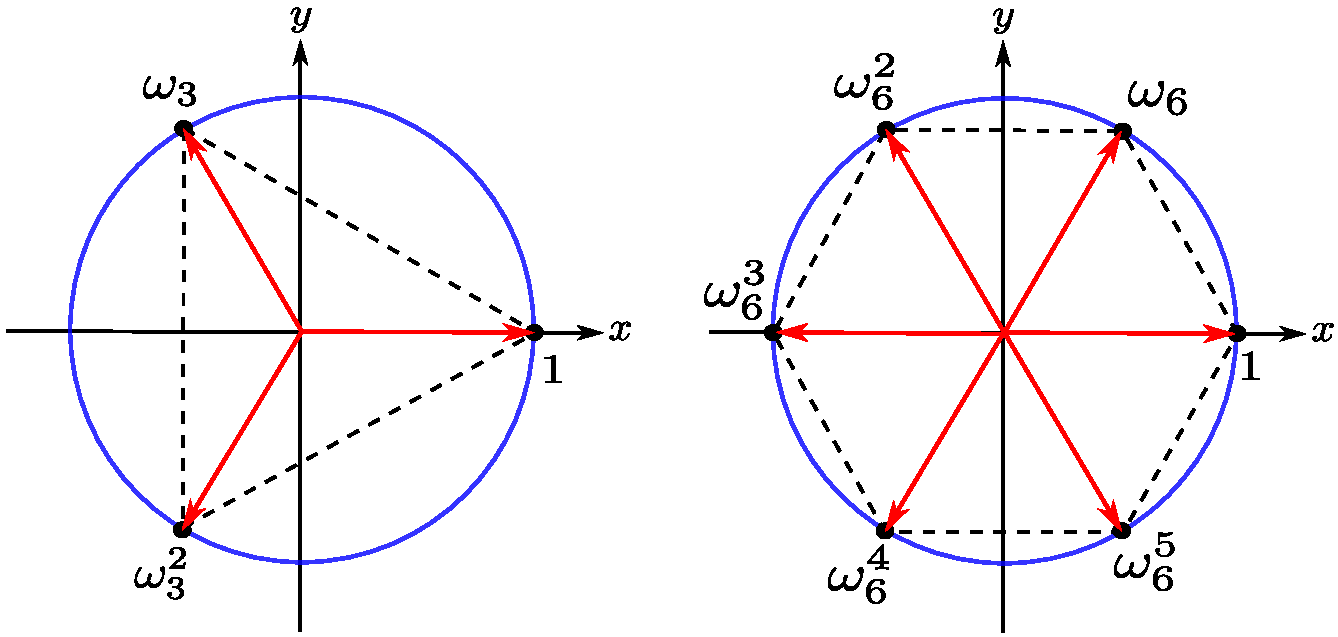
\includegraphics[scale=0.5]{Figuras/RaizUnidad.pdf}
    \caption{Raíces $n$-ésima de la unidad para $n = 3$ y $n = 6$.}
    \label{RaizUno}
\end{figure}

\end{enumerate}

\section{Topología de los números complejos}

 Recordemos que si $z \in \mathbb{C}$, entonces el módulo de $z$ satisface las siguientes propiedades:

\begin{enumerate}
\item $|z| \geq 0$.

\item $ |z| = 0 ~\Leftrightarrow~ z = 0$.

\item Si $z_1, z_2 \in \mathbb{C}$, entonces $|z_1 z_2| = |z_1|\, |z_2|$.

\item Si $z_1, z_2 \in \mathbb{C}$, entonces $|z_1 + z_2| \leq |z_1| + |z_2|$.
\end{enumerate}

Utilizando el módulo, se define la siguiente función
$$d: \mathbb{C} \times \mathbb{C} \longrightarrow \mathbb{R}, \quad (z_1,z_2) \mapsto d(z_1,z_2) = |z_1 - z_2|.$$

Para $z_1, z_2, z_3 \in \mathbb{C}$, notemos que $d$ satisface:

\begin{itemize}
\item[D1.] $d(z_1,z_2) \geq 0$.

\item[D2.] $d(z_1,z_2) = 0 ~\Leftrightarrow~ z_1 = z_2$.

\item[D3.] $d(z_1,z_2) = d(z_2, z_1)$.

\item[D4.] $d(z_1,z_3) \leq d(z_1,z_2) + d(z_2,z_3)$.
\end{itemize}

Por las propiedades satisfechas por la función $d$, ésta se llama \textbf{distancia o métrica} en $\mathbb{C}$, implicando que el par $(\mathbb{C},d)$ es un \textbf{espacio métrico}.

\begin{defi}
Sea $z_0 \in \mathbb{C}$ fijo y sea $\varepsilon >0$ un número real dado. El conjunto
$$B(z_0, \varepsilon) = \{z \in \mathbb{C} ~:~ d(z,z_0) = |z-z_0| < \varepsilon\}$$

se llama \textbf{bola abierta o vecindad o disco abierto de centro $z_0$ y radio $\varepsilon$}.
\end{defi}

Notemos que $B(z_0, \varepsilon)$ corresponde al lugar geométrico de un círculo de centro $z_0$ y radio $\varepsilon$ que no contiene su circunferencia.

\begin{figure}[H]
    \centering
    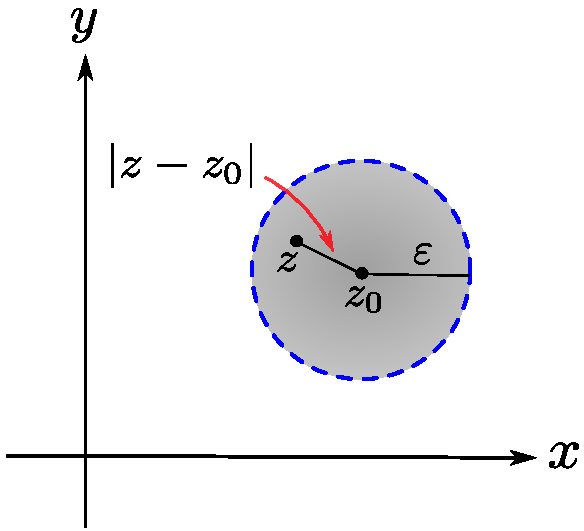
\includegraphics[scale=0.55]{Figuras/BolaAbierta.pdf}
    \caption{Bola abierta de centro $z_0$ y radio $\varepsilon$ en el plano complejo.}
    \label{BolaAbierta}
\end{figure}

\begin{defi}
Sea $A$ un subconjunto de $\mathbb{C}$ y sea $z \in \mathbb{C}$. Diremos que $z$ es un \textbf{punto interior de $A$} si 
$$\exists \varepsilon >0 :~ B(z,\varepsilon) \subseteq A.$$

Notar que, en este caso, $z \in A.$
\end{defi}

\begin{defi}
Un subconjunto $A$ en $\mathbb{C}$ se llama \textbf{conjunto abierto} si todos sus puntos son puntos interiores de $A$, en otras palabras, si
$$(\forall z \in A)(\exists \varepsilon(z) >0)(B(z, \varepsilon(z)) \subseteq A).$$
\end{defi}

\begin{defi}
Sea $A$ un subconjunto de $\mathbb{C}$ y sea $z \in \mathbb{C}$. Diremos que $z$ es un \textbf{punto exterior de $A$} si
$$\exists \varepsilon >0 :~ B(z,\varepsilon) \cap A = \emptyset.$$

Notar que, en este caso, $z \notin A$.
\end{defi}

\begin{defi}
Sea $A$ un subconjunto de $\mathbb{C}$ y sea $z \in \mathbb{C}$. Diremos que $z$ es un \textbf{punto de frontera de $A$} si $z$ no es punto interior y tampoco punto exterior de $A$. El conjunto de todos los puntos frontera de $A$ se llama \textbf{frontera de $A$} y se denota por $Fr(A)$. 
\end{defi}

\begin{ejemplo}
El conjunto $\{z \in \mathbb{C} : |z| = 1\}$ es la frontera de: $\{z \in \mathbb{C} : |z|<1\}$ y $\{z \in \mathbb{C} : |z|\leq 1\}$.
\end{ejemplo}

\begin{defi}
Un subconjunto $F$ de $\mathbb{C}$ se llama \textbf{conjunto  cerrado} si su complemento $F^c = \mathbb{C} \setminus F$ es abierto.
\end{defi}

\begin{defi}
Sea $S$ un subconjunto de $\mathbb{C}$, se llama \textbf{clausura o adherencia de $S$} al conjunto $S \cup Fr(S)$ y se denota por $\overline{S}$.
\end{defi}

\textbf{Observación:} Existen conjuntos que no son ni abiertos ni cerrados, por ejemplo, $\{z \in \mathbb{C} : 0 < |z| \leq 1\}$. En cambio, el conjunto de los números complejos es abierto y cerrado a la vez.

\begin{defi}
Un subconjunto $S$ de $\mathbb{C}$ se llama \textbf{conjunto conexo} si cualquier par de puntos $z_1, z_2 \in S$ puede unirse por un camino poligonal consistente de un número finito de segmentos unidos por sus punto iniciales y finales y que se encuentra enteramente contenido en $S$. 
\end{defi}

\begin{ejemplo}
Algunos ejemplos de conjuntos conexos son: $\{z \in \mathbb{C} : |z| <1\}$; $\{z \in \mathbb{C} : |z| \leq 1\}$; $\{z \in \mathbb{C} : 1 < |z| <2 \}$, ver figura \ref{Conexo}.

\begin{figure}[H]
    \centering
    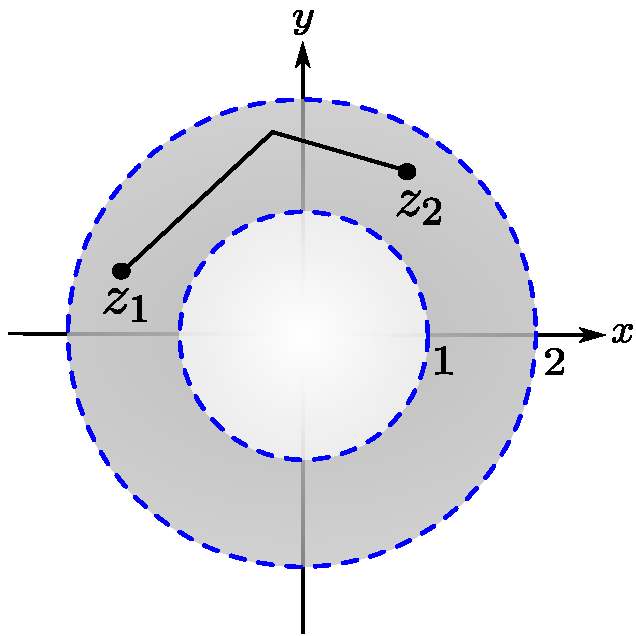
\includegraphics[scale=0.45]{Figuras/EjemploConexo.pdf}
    \caption{Gráfica del conjunto conexo $\{z \in \mathbb{C} : 1 < |z| <2 \}$.}
    \label{Conexo}
\end{figure}

\end{ejemplo}

\begin{defi}
Un conjunto conexo abierto se llama \textbf{dominio} y un dominio con alguna o ninguna o toda su frontera se llama \textbf{región}.
\end{defi}

\textbf{Observación:} Note que cualquier vecindad es un dominio.

\begin{defi}
Un subconjunto $S$ de $\mathbb{C}$ se llama \textbf{conjunto acotado} si existe $M >0$ tal que

$$(\forall z \in S)(|z| \leq M).$$

En caso contrario, se llamará conjunto no acotado.
\end{defi}

\begin{ejemplo}
El primer cuadrante del plano, una recta, el complemento de cualquier vecindad, etc, son ejemplos de conjuntos no acotados.
\end{ejemplo}

\begin{defi}
Sea $A$ un subconjunto de $\mathbb{C}$ y sea $z_0 \in \mathbb{C}$. Diremos que $z_0$ es un \textbf{punto de acumulación de $A$} si

$$(\forall \varepsilon > 0)([B(z_0, \varepsilon) \setminus \{z_0\} ]\cap A \neq \emptyset).$$ 
\end{defi}

\section{El punto al infinito}

A menudo es conveniente considerar, junto con el plano complejo, un punto especial llamado \textbf{punto al infinito} y que lo denotaremos por $\infty$. Para visualizar este punto, consideraremos una esfera unitaria $S$ centrada en el origen del sistema rectangular $xyz$ elegido para el espacio $\mathbb{R}^3$ y asumamos que el plano complejo es el plano $xy$ que pasa a través del ecuador.

\begin{figure}[H]
    \centering
    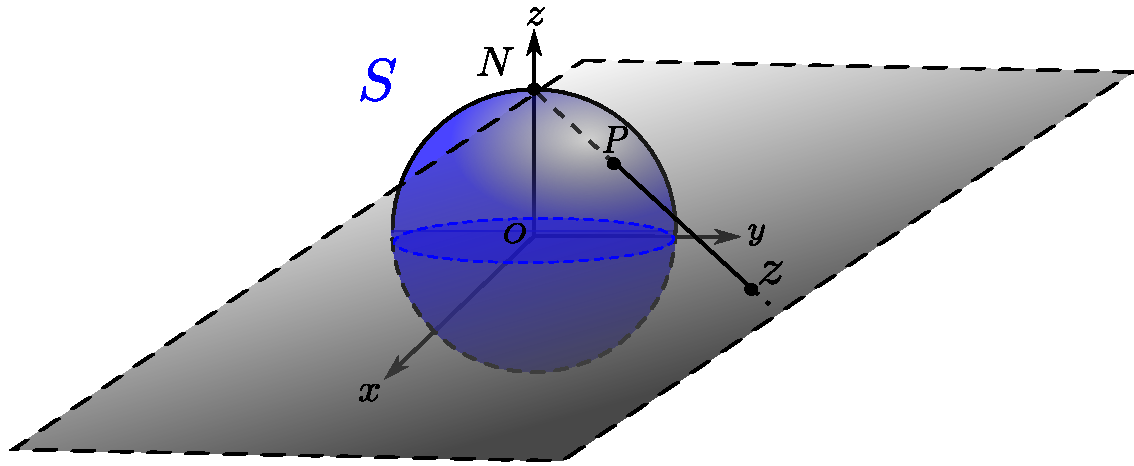
\includegraphics[scale=0.5]{Figuras/EsferaRiemann.pdf}
    \caption{Esfera de Riemann.}
    \label{EsferaRiemann}
\end{figure}

Observar que la recta en el espacio, que pasa por el punto $N = (0,0,1)$ (polo norte de la esfera) y un punto $z$ dado en el punto complejo, determina un único punto $P$ de la esfera. De igual manera, la recta que pasa por el polo norte y un punto dado $P$ en la esfera, determina un único punto $z$ del plano complejo. En otras palabras, existe una aplicación biyectiva
$$f: S - \{N\} \longrightarrow \mathbb{C}, \quad P \mapsto z.$$

Ahora, si al plano complejo le agregamos un elemento, que lo denotaremos por el símbolo $\infty$, el nuevo conjunto $C \cup \{\infty\} = \overline{\mathbb{C}}$ lo llamamos \textbf{plano extendido}. De esta manera, la aplicación $f$ puede extenderse también a $N$ de la siguiente forma:
$$f: S  \longrightarrow \mathbb{C}, \quad P \mapsto \left\{ \begin{array}{ccl}
z &,& P \neq N \\
\infty &,& P = N
\end{array} \right. .$$

Este proceso de correspondencia se llama \textbf{proyección estereográfica} y la esfera es conocida por \textbf{esfera de Riemann}.

Con el fin de extender la adición y multiplicación en el plano complejo al plano extendido, definiremos las siguientes reglas:
\begin{eqnarray*}
z + \infty = \infty &;& z \cdot \infty = \infty,  ~ z \neq 0\\
\infty + \infty = \infty &;& \infty \cdot \infty = \infty.
\end{eqnarray*}

Observar que la imagen del hemisferio norte menos su polo de la esfera de Riemann corresponde al exterior de la bola unitaria y recíprocamente. Además, para un pequeño número positivo $\varepsilon$, aquellos puntos del plano complejo exteriores a la circunferencia $|z| = \frac{1}{\varepsilon}$  corresponden a puntos de la esfera próximos a $N$. Llamaremos al conjunto $B(\infty, \frac{1}{\varepsilon}) = \{z \in \mathbb{C} : |z| > \frac{1}{\varepsilon}\}$ un \textbf{entorno de $\infty$}.
\chapter{Funciones analíticas}

\section{Funciones de variable compleja}

\begin{defi}
Sea $S \subseteq \mathbb{C}$. Una \textbf{función} $f$ definida sobre $S$ es una regla que asigna a cada $z$ en $S$ un número complejo $w$ ($f: S \longrightarrow \mathbb{C}$). El número $w$ se llama \textbf{imagen} de $z$ y se denota por
$$w = f(z).$$

El conjunto $S$ se llama el \textbf{dominio} de $f$.
\end{defi}

De aquí en adelante, asumiremos que el dominio de la función $S$ es el más grande posible subconjunto de $\mathbb{C}$ tal que $f(z)$ esté bien definida.

\begin{ejemplo}
La función 
$$f(z) = \frac{1}{z}$$

tiene como dominio al conjunto de todos los números complejos distintos de cero.
\end{ejemplo}

\begin{defi}
La \textbf{gráfica} de una función compleja $f: S \longrightarrow \mathbb{C}$ es el conjunto
$$graf(f) = \{(z,f(z)) : z \in S\}.$$
\end{defi}

\textbf{Observación:} La gráfica de $f$ es un subconjunto de $\mathbb{R}^4$, en consecuencia, no tenemos una visualización de la gráfica. Sin embargo, podemos desplegar alguna información de la función observando la imagen de subconjuntos de su dominio.

En este caso, tal como se observa en la figura \ref{FUncionCompleja}, es conveniente disponer de dos planos complejos separados, donde uno de ellos contiene su dominio y el otro a su recorrido.

\begin{figure}[H]
    \centering
    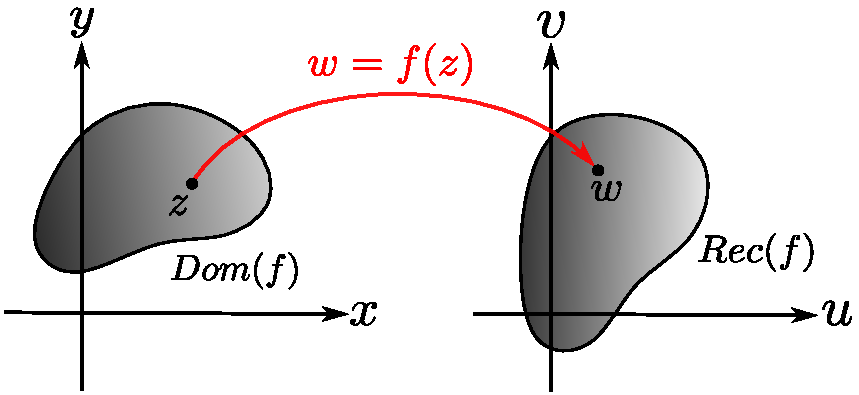
\includegraphics[scale=0.65]{Figuras/FuncionDomRec.pdf}
    \caption{Gráfica del dominio y recorrido de una función compleja.}
    \label{FUncionCompleja}
\end{figure}

\begin{ejemplo}
Consideremos la función $f(z) = iz$ y analicemos la imagen de la circunferencia
$$C_r = \{z \in \mathbb{C} : |z| = r \}; ~ r > 0.$$

Si $z = r (\cos \theta + i \sin \theta) \in C_r$, entonces
\begin{eqnarray*}
f(z) &=& iz \\
&=& \left( \cos \frac{\pi}{2} + i \sin \frac{\pi}{2} \right) r (\cos \theta + i \sin \theta) \\
&=& r \left[ \cos\left( \theta + \frac{\pi}{2} \right) + i \sin \left( \theta + \frac{\pi}{2}  \right) \right] = w.
\end{eqnarray*}

Luego, la imagen $w$ tiene igual magnitud que $z$ y ha sido rotada en $\frac{\pi}{2}$ radianes. En consecuencia,
$$f(C_r) = C_r.$$
\end{ejemplo}

\begin{ejemplo}
Bosqueje la imagen de los conjuntos dados respecto de las funciones:

\begin{enumerate}
\item $f(z) = |z| + i Im(z), ~ C_r$.

\item $f(z) = z^2, ~ B = \{z = (x,y) : 0 \leq x \leq y\}$.
\end{enumerate}

\textbf{Solución:}

\begin{enumerate}
\item La gráfica del dominio y el recorrido están dadas a continuación.

\begin{figure}[H]
    \centering
    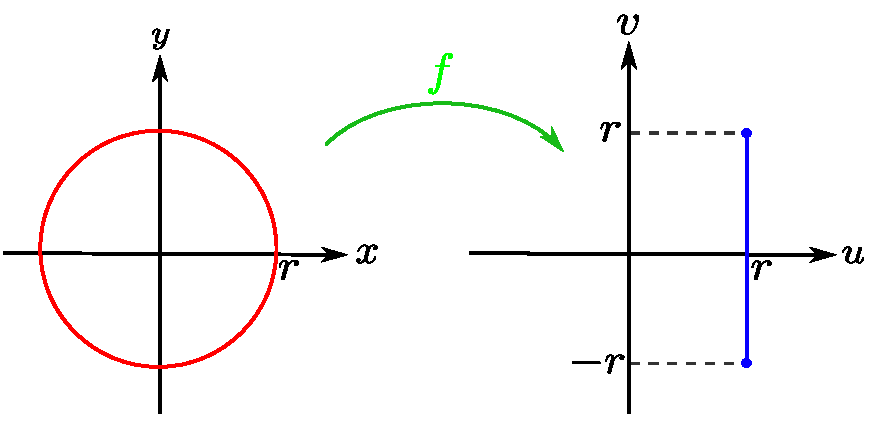
\includegraphics[scale=0.6]{Figuras/EjemploFuncion1.pdf}
    \caption{Imagen de la circunferencia centrada en el origen de radio $r$ para $f(z) = |z| + i Im(z)$.}
    \label{EjemploFuncion1}
\end{figure}

\item Si $z = r e^{i\theta} \in B\setminus \{0\}$, entonces
$$f(z) = z^2 = r^2 e^{i2\theta}$$

con 
$$\frac{\pi}{4} \leq \theta \leq \frac{\pi}{2} \Leftrightarrow \frac{\pi}{2} \leq 2\theta \leq \pi.$$

Como $f(0) = 0$, $f(B) = \{ z= (x,y) : x \leq 0, y \geq 0\}$ y la gráfica del dominio y el recorrido nos queda:

\begin{figure}[H]
    \centering
    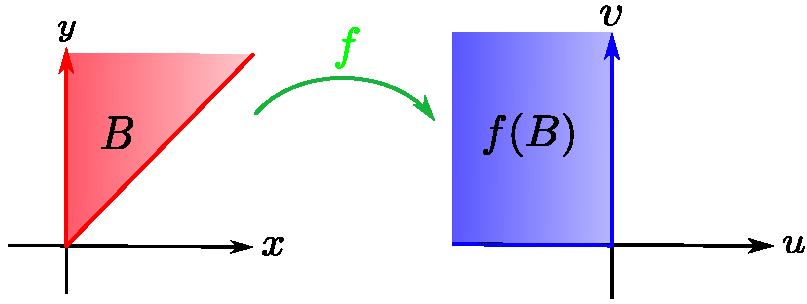
\includegraphics[scale=0.7]{Figuras/EjemploFuncion2.pdf}
    \caption{Imagen de $B$ para $f(z) = z^2$.}
    \label{EjemploFuncion2}
\end{figure}

\end{enumerate}
\end{ejemplo}

\section{Límites} 

\begin{defi}
Sea $f: A \subseteq \mathbb{C} \longrightarrow \mathbb{C}$ una función compleja y sea $z_0 \in \mathbb{C}$ un punto de acumulación de $A$. Diremos que $f$ se aproxima a $w_0$ cuando $z \in A$ se aproxima a $z_0$ si
\begin{equation}
(\forall \varepsilon >0 )(\exists \delta >0) (0 < |z-z_0| < \delta ~\wedge~ z \in A ~\Rightarrow~ |f(z) -w_0| < \varepsilon). \label{defiLimite}
\end{equation}

Denotaremos a \eqref{defiLimite} por
$$\lim_{z \to z_0} f(z) = w_0.$$
\end{defi}

\textbf{Observación:} Notemos que \eqref{defiLimite} puede reescribirse en los siguientes términos:
$$(\forall \varepsilon >0 )(\exists \delta >0) (z \in (B(z_0, \delta)\setminus \{z_0\}) \cap A ~\Rightarrow~ f(z) \in B(w_0, \varepsilon))$$

y geométricamente, se ve como sigue:

\begin{figure}[H]
    \centering
    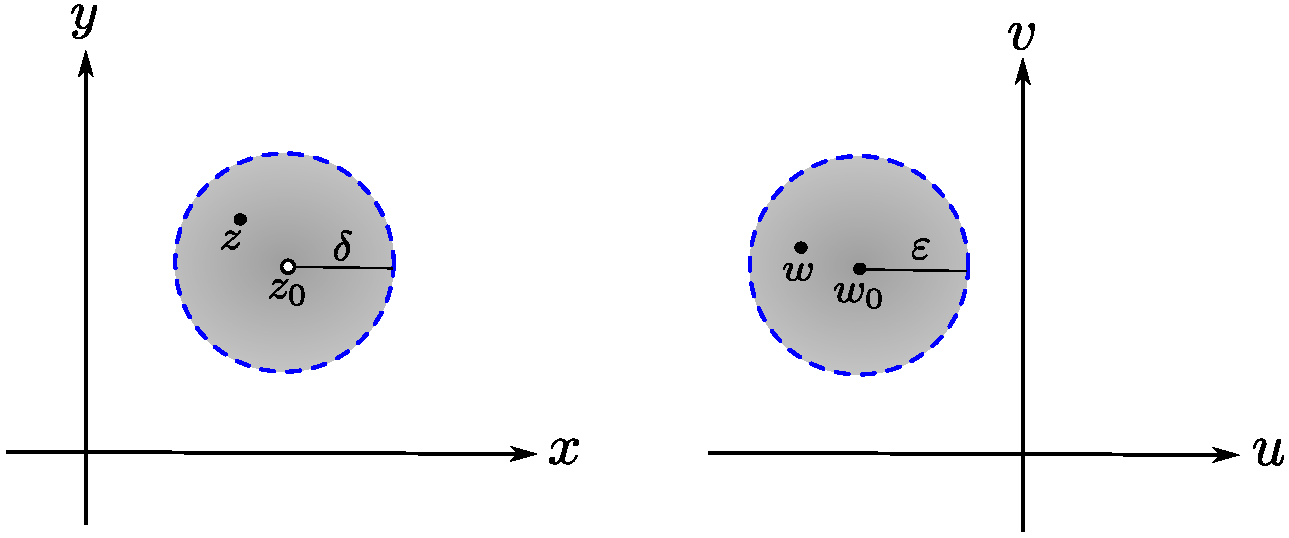
\includegraphics[scale=0.5]{Figuras/DefLimite.pdf}
    \caption{Interpretación geométrica del límite.}
    \label{DefLimite}
\end{figure}

\begin{ejemplo}
Demuestre que
$$\lim_{z \to 1} \frac{iz}{2} = \frac{i}{2}.$$

\textbf{Solución:} En efecto, notemos primero que $A =  \mathbb{C}$, luego para cualquier $\varepsilon > 0$, debemos ser capaces de encontrar $\delta >0$ de manera que si $0 < |z-1| < \delta$, entonces
$$\left| \frac{iz}{2} - \frac{i}{2}\right| < \varepsilon.$$

Trabajando la expresión
$$\left| \frac{iz}{2} - \frac{i}{2}\right| = \left| \frac{i}{2} (z-1) \right| = \frac{1}{2} |z-1|.$$

Luego, eligiendo $\delta = 2\varepsilon$, tenemos para $0 < |z-1|< 2\varepsilon$ que
$$\left| \frac{iz}{2} - \frac{i}{2}\right| =  \frac{1}{2} |z-1| < \frac{1}{2} 2 \varepsilon = \varepsilon.$$
\end{ejemplo}

\textbf{Observación:} Notemos que una función compleja $f: A \subseteq \mathbb{C} \longrightarrow \mathbb{C}$ no es otra cosa que una función $f: A \subseteq \mathbb{R}^2 \longrightarrow \mathbb{R}^2$, asi que todo lo que se estudió en el curso de Cálculo III es aplicable a estas funciones.
\\

En el ejemplo,
$$f(z) = f(x,y) = \frac{1}{2}(0,1)(x,y) = \frac{1}{2}(-y,x)$$

y
$$z \to 1 ~\Rightarrow~ (x,y) \to (1,0).$$

Así,
$$\lim_{z \to 1} f(z) = \lim_{(x,y) \to (1,0)} \frac{1}{2} (-y,x) = \frac{1}{2}(0,1) = \frac{i}{2}.$$

\begin{ejemplo}
Mostrar que
$$\lim_{z \to 2i} (2x+iy^2)= 4i.$$

\textbf{Solución:}
\begin{equation*}
\lim_{z \to 2i} (2x+iy^2) = \lim_{(x,y) \to(0,2)} (2x,y^2) 
= (0,4) = 4i.
\end{equation*}

\end{ejemplo}

\begin{teorema}[Existencia y unicidad del límite]
Si $\lim\limits_{z \to z_0} f(z) = w_0$ y $\lim\limits_{z \to z_0} f(z) = w_1$, entonces $w_0 = w_1$.
\end{teorema}

\begin{proof}
Por hipótesis, dado $\varepsilon >0$, existen $\delta_1>0$ y $\delta_2 >0$ tales que 
\begin{eqnarray*}
0< |z-z_0| < \delta_1 ~\wedge~ z \in Dom(f) ~\Rightarrow ~ |f(z)-w_0| < \frac{\varepsilon}{2}, \\
0< |z-z_0| < \delta_2 ~\wedge~ z \in Dom(f) ~\Rightarrow ~ |f(z)-w_1| < \frac{\varepsilon}{2}.
\end{eqnarray*}

Escogemos $\delta = \min\{\delta_1, \delta_2\}$ (para que ambas condiciones  se verifiquen) y se cumple que
\begin{eqnarray*}
|w_0-w_1| &=& |(f(z) - w_0) - (f(z) - w_1)| \\
&\leq & |f(z) - w_0| + |f(z) - w_1| < \varepsilon .
\end{eqnarray*}

Como $\varepsilon$ es un número positivo arbitrario, tenemos que $|w_1 - w_2|$ es una cota inferior de $]0, + \infty[$. Entonces, por el axioma del supremo, existe $ \inf]0, + \infty[$ y 
$$|w_1 - w_2| \leq  \inf]0, + \infty[ = 0 \Rightarrow  0 \leq |w_1 - w_2| \leq 0 ~\Rightarrow~ |w_1 - w_2| = 0 ~\Rightarrow~ w_1 = w_2.$$

\end{proof}

\begin{propo} \label{LimitesParteRealIm}
Supongamos que $f(z) = u(x,y) +i v(x,y)$, $z_0 = x_0 +iy_0$ y $w_0 = u_0 +iv_0$. Entonces,
$$\lim_{z \to z_0} f(z) = w_0 ~\Leftrightarrow~ \left\{ \begin{array}{c}
\lim\limits_{(x,y) \to (x_0,y_0)} u(x,y) = u_0 \\
\lim\limits_{(x,y) \to (x_0,y_0)} v(x,y) = v_0
\end{array} \right. .$$
\end{propo}

\begin{proof}
En Cálculo III se estudió que las normas 
$$\norm{(x,y)}_2 = \sqrt{x^2+ y^2}~~\mbox{y}~~\norm{(x,y)}_{\infty} = \max\{|x|,|y|\}$$

satisfacen las desigualdades
\begin{eqnarray}
\norm{(x,y)}_{\infty} = \max\{|x|,|y|\} &\leq & \norm{(x,y)}_2. \label{limite1} \\
\norm{(x,y)}_2 &\leq & \sqrt{2} \norm{(x,y)}_{\infty}.\label{limite2}
\end{eqnarray} 

Supongamos que $\lim\limits_{z \to z_0} f(z) = w_0$. Entonces, dado $\varepsilon > 0$, $\exists \delta > 0$ tal que
$$0< |z-z_0| < \delta, z \in Dom(f) ~\Rightarrow ~ |f(z)-w_0| < \varepsilon. $$

Como $|z-z_0| = \norm{(x,y) - (x_0,y_0)}_2$ y 
$$|u(x,y) - u_0| \leq |f(z) - w_0| ~\wedge~|v(x,y) - v_0| \leq |f(z) - w_0|, $$

se verifica que
\begin{eqnarray*}
0< \norm{(x,y) - (x_0,y_0)}_2 < \delta, (x,y) \in Dom(f) ~\Rightarrow ~ |u(x,y) - u_0| \leq |f(z) - w_0| < \varepsilon . \\
0< \norm{(x,y) - (x_0,y_0)}_2 < \delta, (x,y) \in Dom(f) ~\Rightarrow ~ |v(x,y) - v_0| \leq |f(z) - w_0| < \varepsilon . 
\end{eqnarray*}

Hemos probado así, la implicancia hacia la derecha.

Supongamos ahora que
$$\lim_{(x,y) \to (x_0,y_0)} u(x,y) = u_0  ~~\mbox{y}~~\lim_{(x,y) \to (x_0,y_0)} v(x,y) = v_0.$$

Es decir, dado $\varepsilon >0$, $\exists \delta_1, \delta_2 >0$ tales que
\begin{eqnarray*}
0< \norm{(x,y) - (x_0,y_0)}_2 < \delta_1 , (x,y) \in Dom(f) ~\Rightarrow ~ |u(x,y) - u_0| < \frac{\varepsilon}{\sqrt{2}}, \\
0< \norm{(x,y) - (x_0,y_0)}_2 < \delta_2 , (x,y) \in Dom(f) ~\Rightarrow ~ |v(x,y) - v_0|  < \frac{\varepsilon}{\sqrt{2}} . 
\end{eqnarray*}

Escogiendo $\delta = \min\{\delta_1, \delta_2\}$, se verifica:
\begin{eqnarray*}
0 < |z - z_0| = \norm{(x,y) - (x_0,y_0)}_2 < \delta, z \in Dom(f) &\Rightarrow & |f(z) -w_0| \\
&=& \norm{(u(x,y), v(x,y)) - (u_0,v_0)}_2 \\
&\leq & \sqrt{2} \max\{|u(x,y) -u_0|, |v(x,y) - v_0|\} \\
&< & \sqrt{2} \frac{\varepsilon}{\sqrt{2}} = \varepsilon.
\end{eqnarray*}

Hemos probado así, la implicancia hacia la izquierda.

\end{proof}

\begin{teorema}[Álgebra de límites] \label{AlgebraLimites}
Supongamos que
$$\lim_{z \to z_0} f(z) = w_0 ~~\mbox{y}~~ \lim_{z \to z_0} F(z)= W_0.$$

Entonces,

\begin{enumerate}
\item $\lim\limits_{z \to z_0} [f(z) + F(z)] = w_0 + W_0.$

\item $\lim\limits_{z \to z_0} [f(z)  F(z)] = w_0  W_0.$

\item $\lim\limits_{z \to z_0} \left[ \frac{f(z)}{F(z)} \right] = \frac{w_0}{W_0}$, siempre que $W_0 \neq 0$.
\end{enumerate}
\end{teorema}

\begin{proof}
\

\begin{enumerate}

\item Por hipótesis, tenemos que dado $\varepsilon >0$, $\exists \delta_1, \delta_2 >0$ tales que
\begin{eqnarray*}
 0 < |z-z_0| <  \delta_1, z \in Dom(f+F) ~\Rightarrow~ |f(z) - w_0| < \frac{\varepsilon}{2},\\
  0 < |z-z_0| <  \delta_2, z \in Dom(f+F) ~\Rightarrow~ |F(z) - W_0| < \frac{\varepsilon}{2}.
\end{eqnarray*}

Eligiendo $\delta = \min\{ \delta_1, \delta_2 \}$:
\begin{eqnarray*}
  0 < |z-z_0| <  \delta, z \in Dom(f+F)  & \Rightarrow & |(f(z) + F(z)) - (w_0 + W_0)| \\
&= & |(f(z) - w_0) + (F(z) - W_0)| \\
& \leq & |f(z) - w_0| + |F(z) - W_0| \\
&< & \frac{\varepsilon}{2} + \frac{\varepsilon}{2} = \varepsilon.
\end{eqnarray*}

\item Escribamos
\begin{eqnarray*}
|f(z)F(z) - w_0 W_0| &\leq & |f(z)F(z) - f(z)W_0| +|f(z)W_0 - w_0 W_0| \\
&=& |f(z)| |F(z) -W_0| + |f(z) - w_0||W_0|.
\end{eqnarray*}

Queremos estimar cada término. Para hacerlo, la hipótesis nos permite escoger $\delta_1 > 0$ tal que
$$0 < |z-z_0| < \delta_1, z \in Dom(f\cdot F) ~\Rightarrow~ |f(z) -w_0| < 1 ~\Rightarrow~ |f(z)| < |w_0| + 1.$$

Dado $\varepsilon >0$, podemos escoger $\delta_2 > 0$, tal que
$$0 <|z-z_0| < \delta_2, z \in Dom(f\cdot F) ~\Rightarrow~ |f(z)-w_0| < \left\{ \begin{array}{cl}
\frac{\varepsilon}{2 |W_0|},& W_0 \neq 0 \\
1,& W_0 = 0
\end{array} \right. .$$

y $\delta_3 >0$ tal que
$$0 < |z-z_0| < \delta_3,  z \in Dom(f\cdot F)  ~\Rightarrow~ |F(z) -W_0| < \frac{\varepsilon}{2(|w_0| +1)}.$$

Sea $\delta = \min\{\delta_1, \delta_2, \delta_3\}$, entonces
\begin{eqnarray}
0 < |z-z_0| < \delta, z \in Dom(f\cdot F) &\Rightarrow & |f(z)F(z) - w_0 W_0| \nonumber \\
&\leq & |f(z)| |F(z) -W_0| + |f(z) - w_0||W_0| \nonumber \\
&< & \frac{\varepsilon}{2(|w_0| +1)}|f(z)| + \frac{\varepsilon}{2|W_0|} |W_0 | ~~~ (W_0 \neq 0)\label{producto} \\
&< & \frac{\varepsilon}{2} + \frac{\varepsilon}{2} = \varepsilon. \nonumber
\end{eqnarray}

Si en \eqref{producto}, $W_0 = 0$, se reemplaza el segundo término por cero, cumpliéndose también la definición de límite para el producto.

\item Demostremos primero que
$$\lim_{z \to z_0} \left[ \frac{1}{F(z)} \right] = \frac{1}{W_0}, \quad W_0 \neq 0. $$

Por hipótesis, $\exists \delta_1 >0$ tal que
\begin{eqnarray*}
0 < |z-z_0| < \delta_1, z \in Dom(1/F) &\Rightarrow & |F(z) -W_0| < \frac{|W_0|}{2} \\
& \Rightarrow & ||F(z)| - |W_0|| < \frac{|W_0|}{2} \\
& \Leftrightarrow &  - \frac{|W_0|}{2} + |W_0|    < |F(z)| < \frac{|W_0|}{2} + |W_0| \\
& \Rightarrow & \frac{|W_0|}{2} < |F(z)|  ~ \Rightarrow  \frac{1}{|F(z)|} < \frac{2}{|W_0|}.
\end{eqnarray*}

Dado $\varepsilon >0$, $\exists \delta_2 > 0$ tal que
$$0 < |z-z_0| < \delta_2, z \in Dom(1/F) ~ \Rightarrow ~  |F(z)-W_0| < \frac{|W_0|^2}{2} \varepsilon .$$

Escogiendo $\delta = \min \{\delta_1, \delta_2\}$, se verifica que
\begin{eqnarray*}
0 < |z-z_0| < \delta, z \in Dom(1/F) &\Rightarrow & \left| \frac{1}{F(z)} -\frac{1}{W_0}  \right| \\
&=& \frac{1}{|F(z)|} \frac{1}{|W_0|} |F(z) -W_0| \\
&< & \frac{2}{|W_0|^2} \cdot \frac{|W_0|^2}{2} \varepsilon  = \varepsilon . 
\end{eqnarray*}

Luego, por lo demostrado en el ítem $2.$, se tiene que
$$\lim_{z \to z_0} \left[ \frac{f(z)}{F(z)} \right] =\lim_{z \to z_0} \left[ f(z) \cdot \frac{1}{F(z)} \right] = \frac{w_0}{W_0}. $$
\end{enumerate}
\end{proof}

\begin{propo}
$$\lim_{z \to z_0} f(z) = w_0 \Rightarrow\lim_{z \to z_0} |f(z)| = |w_0|. $$
\end{propo}

\begin{proof}
Por hipótesis, dado $\varepsilon >0$, $\exists \delta >0$ tal que
$$0 < |z-z_0| < \delta, z \in Dom(f) ~\Rightarrow ~ |f(z) - w_0| < \varepsilon. $$

Luego,
\begin{eqnarray*}
0 < |z-z_0| < \delta, z \in Dom(f) &\Rightarrow & ||f(z)| - |w_0||  \\
&\leq & |f(z) -w_0| < \varepsilon.
\end{eqnarray*}
\end{proof}

\begin{defi}
Sea $f: A \subseteq \mathbb{C} \longrightarrow \mathbb{C}$ una función compleja y supongamos que $\infty$ es punto de acumulación de $A$. Entenderemos por
$$\lim_{z \to \infty} f(z) = L$$

a lo siguiente:
$$(\forall \varepsilon >0)(\exists M >0)(|z|> M ~\wedge~ z \in A ~\Rightarrow~ |f(z) -L| < \varepsilon).$$
\end{defi}

\begin{ejemplo}
Mostrar que 
$$\lim_{z \to \infty} \frac{1}{z} = 0.$$

\textbf{Solución:} Dado $\varepsilon >0$,  elegimos $M = \frac{1}{\varepsilon} > 0$ tal que
$$|z| > M ~\Rightarrow~ \left| \frac{1}{z} -0 \right| = \left| \frac{1}{z} \right| = \frac{1}{|z|} < \frac{1}{M} = \varepsilon
.$$
\end{ejemplo}


\begin{defi}
Sea $f: A \subseteq \mathbb{C} \longrightarrow \mathbb{C}$ una función compleja y sea $z_0 \in \mathbb{C}$ un punto de acumulación de $A$. Entenderemos por
$$\lim_{z \to z_0} f(z) = \infty$$

a lo siguiente:
$$(\forall M >0)(\exists \delta >0)(0 < |z-z_0| < \delta ~\wedge~ z \in A ~\Rightarrow ~ |f(z)| >M).$$
\end{defi}

\begin{ejemplo}
Mostrar que 
$$\lim_{z \to 0} \frac{1}{z} = \infty.$$

\textbf{Solución:} Dado $M >0$,  elegimos $\delta = \frac{1}{M} > 0$ tal que
$$0 < |z-0| < \delta ~\Rightarrow~ \left| \frac{1}{z} -0 \right| = \left| \frac{1}{z} \right| = \frac{1}{|z|} > M
.$$
\end{ejemplo}

\textbf{Observación:} Existe una definición similar para
$$\lim_{z \to \infty} f(z) = \infty$$

cuando $\infty$ es punto de acumulación de $A$ y que significa:
$$(\forall M >0)(\exists K >0) (|z|> K ~\wedge~ z \in A ~\Rightarrow~ |f(z)| > M).$$

\section{Continuidad}

\begin{defi}
Sea $f: A \subseteq \mathbb{C} \rightarrow \mathbb{C}$ una función compleja y $z_0 \in A$. Diremos que $f$ es \textbf{continua} en $z_0$ si
$$\lim_{z \to z_0} f(z) = f(z_0),$$

o, equivalentemente, 
$$(\forall \varepsilon >0)(\exists \delta >0)(0 < |z-z_0| < \delta ~\wedge~ z \in A ~\Rightarrow~ |f(z) - f(z_0)| < \varepsilon).$$
\end{defi}

\textbf{Observación:} Al igual que antes, al considerar a $f$ como una función $f: A \subseteq \mathbb{R}^2 \longrightarrow \mathbb{R}^2$, usaremos toda información relacionada a la continuidad estudiada en Cálculo III.
\\

Decimos que una función $f: A\subseteq \mathbb{C} \rightarrow \mathbb{C}$ es continua en $A$, o simplemente continua, si $f$ es continua en cada $z_0 \in A$.

\begin{ejemplo}
Demuestre la continuidad de $f(z) = z^2 + b $, con $b \in \mathbb{C}$ constante.
\\

\textbf{Solución:} Hay que demostrar que 
$$\lim_{z \to z_0}( z^2+b) = z_0^2 +b.$$

Primero desarrollemos la expresión
$$|z^2 +b - (z_0^2 + b)| = |z^2 -z_0^2| = |z+z_0| \, |z-z_0|.$$

Acotemos $|z+z_0|$, para ello elegimos $\delta < 1$ tal que $|z-z_0|< 1$ y así
$$|z+z_0| = |z-z_0 + 2z_0| \leq |z-z_0| + 2|z_0| < 1 + 2|z_0|$$

y si además, dado $\varepsilon >0$, elegimos $\delta < \min \left\{1, \frac{\varepsilon}{1+2|z_0|} \right\}$, tenemos que
\begin{eqnarray*}
0 < |z-z_0| < \delta &\Rightarrow & |z^2 +b - (z_0^2 + b)| \\
&=& |z+z_0| \, |z-z_0| \\
&< & (1+2|z_0|) |z-z_0| \\
&<& (1+2|z_0|) \frac{\varepsilon}{1+2|z_0|} = \varepsilon.
\end{eqnarray*}
\end{ejemplo}

\begin{teorema}[Álgebra y composición de funciones continuas]
Sean $f: A \subseteq \mathbb{C} \rightarrow \mathbb{C}$ y $g: A \subseteq \mathbb{C} \rightarrow \mathbb{C} $ dos funciones complejas continuas en $z_0 \in A$. Entonces,

\begin{enumerate}
\item $f+g$ es continua en $z_0$.

\item $f\cdot g$ es continua en $z_0$. 

\item $\frac{f}{g}$ es continua en $z_0$, siempre que $g(z_0) \neq 0$.

\item Si $h: B \subseteq \mathbb{C} \rightarrow \mathbb{C}$ es tal que $h \circ f$ existe y $h$ es continua en $f(z_0)$, entonces $h \circ f$ es continua en $z_0$.
\end{enumerate}
\end{teorema}

\begin{proof}
Los ítems $1.$, $2.$ y $3.$ son consecuencias directas del teorema \ref{AlgebraLimites}.
\\

Para demostrar el ítem $4.$, supongamos que $\lim\limits_{z \to z_0} f(z) = f(z_0)$ y $\lim\limits_{w \to w_0} h(w) = h(w_0)$, con $w_0 = f(z_0)$. 

Entonces, dado $\varepsilon > 0$, $\exists \delta >0$ tal que
\begin{equation*}
 0 < |w-w_0| < \delta, w \in B ~\Rightarrow~ |h(w) - h(w_0)| < \varepsilon.
\end{equation*}

Luego, del $\delta$ escogido, $\exists \delta^* >0$ tal que
\begin{equation*}
 0 < |z-z_0| < \delta^*, z \in A ~\Rightarrow~ |f(z) - f(z_0)| < \delta.
\end{equation*}

Eligiendo $\bar{\delta} = \delta^*$, se verifica:
\begin{eqnarray*}
 0 < |z-z_0| < \bar{\delta}, \, z \in A &\Rightarrow &  |f(z) - f(z_0)| = |w-w_0| < \delta, w \in B  \\
 &\Rightarrow & |h(f(z)) - h(f(z_0))| = |h(w) - h(w_0)| < \varepsilon .
\end{eqnarray*}

Por lo tanto, $\lim\limits_{z \to z_0} (h\circ f)(z) = (h \circ f)(z_0)$.

\end{proof}

\section{Derivadas}

\begin{defi}
Sea $f: A \subseteq \mathbb{C} \rightarrow \mathbb{C}$ y $z_0$ un punto interior de $A$. Definiremos la \textbf{derivada} de $f$ en $z_0$, y escribiremos $f'(z_0)$, a la ecuación
\begin{equation}
f'(z_0) = \lim_{z \to z_0} \frac{f(z) - f(z_0)}{z-z_0},\label{derivada}
\end{equation}

cuando este límite exista. Diremos que $f$ es \textbf{derivable} o \textbf{diferenciable} en $z_0$ cuando la derivada exista.
\end{defi}

\textbf{Observación:} Si denotamos por
$$\Delta z = z-z_0,$$

entonces podemos escribir \eqref{derivada} como
$$f'(z_0) = \lim_{\Delta z \to 0} \frac{f(z_0 + \Delta z) - f(z_0)}{\Delta z}.$$

Nótese que al ser $z_0$ un punto interior,  $f$ está definida en un entorno de $z_0$ y así el número $f(z_0 + \Delta z)$ está siempre definido para $|\Delta z|$ suficientemente pequeño. 

\begin{figure}[H]
    \centering
    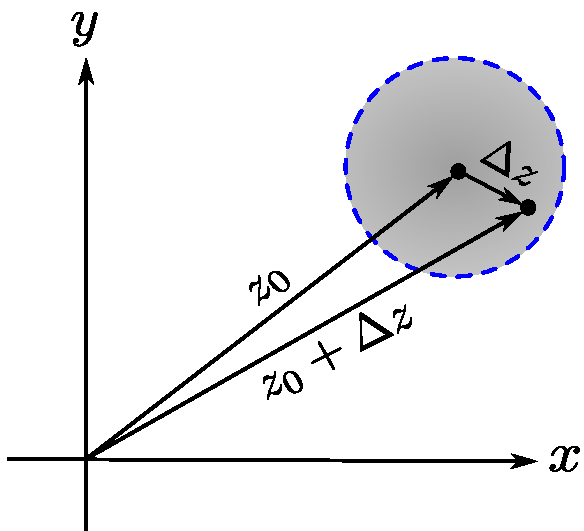
\includegraphics[scale=0.55]{Figuras/DefDerivada.pdf}
    \caption{Interpretación geométrica de la derivada.}
    \label{GeoDerivada}
\end{figure}

Introduciendo el número
$$\Delta w = f(z + \Delta z) - f(z),$$

que denota el cambio en el valor de $f$ correspondiente a un cambio $\Delta z$ en el punto en el que evaluamos $f$. Otra notación para expresar la derivada de $f$ en $z$ es la siguiente:
$$f'(z) = \frac{dw}{dz} = \lim_{\Delta z \to 0} \frac{\Delta w}{\Delta z}.$$

\begin{ejemplo}
Estudiemos la diferenciabilidad de $f(z) = z^2$:
$$\frac{dw}{dz} = \lim_{\Delta z \to 0} \frac{(z + \Delta z)^2 -z^2}{\Delta z} = \lim_{\Delta z \to 0} (2z + \Delta z) = 2z, \quad z \in \mathbb{C}.$$
\end{ejemplo}

\begin{ejemplo}
Estudiemos ahora la diferenciabilidad de $f(z) = |z|^2$:
\begin{eqnarray*}
\frac{\Delta w}{\Delta z} = \frac{f(z + \Delta z) - f(z)}{\Delta z} &=& \frac{|z + \Delta z|^2 - |z|^2}{\Delta z} \\
&=& \frac{(z+\Delta z)\overline{(z+\Delta z)} - z \bar{z}}{\Delta z} \\
&=& \frac{(z+\Delta z)(\bar{z}+\overline{\Delta z}) - z \bar{z}}{\Delta z} \\
&=& \bar{z} + \overline{\Delta z} + z \frac{\overline{\Delta z}}{\Delta z}.
\end{eqnarray*}

Así,
$$f'(0) = \lim_{\Delta z \to 0} \frac{f(0 + \Delta z) - f(0)}{\Delta z} = \lim_{\Delta z \to 0} \overline{\Delta z} =  0.$$

Pero si $z \neq 0$, consideremos las siguientes trayectorias:
$$B_1 = \{z \in \mathbb{C} : Im(\Delta z) = 0\}, \quad B_2 = \{z \in \mathbb{C} : Re(\Delta z) = 0\}$$

tales que $0 \in B_1' \cap B_2'$. Luego,
\begin{eqnarray*}
\lim_{\overset{\Delta z \to 0}{\Delta z \in B_1}} \left[ \bar{z} + \overline{\Delta z} + z \frac{\overline{\Delta z}}{\Delta z} \right] &=& z + \bar{z}, \\
\lim_{\overset{\Delta z \to 0}{\Delta z \in B_2}}\left[ \bar{z} + \overline{\Delta z} + z \frac{\overline{\Delta z}}{\Delta z}\right]&=& -z + \bar{z}. 
\end{eqnarray*}

Por lo tanto, $\frac{dw}{dz}$ no existe para $z \neq 0$.
\end{ejemplo}

\textbf{Observación:} Notemos que al analizar la función $f(z)  = |z|^2$ como función de $\mathbb{R}^2$, tenemos que su parte real e imaginaria, respectivamente, son:
$$u(x,y) = x^2 + y^2, \quad v(x,y) = 0.$$

Ambas tienen derivadas parciales continuas, por tanto, la función \underline{real} es diferenciable en todo punto $(x,y) \in \mathbb{R}^2$.

\begin{ejemplo}
Las derivadas de $f(z) = c = cte$ y $g(z) = z$ son $f'(z) = 0$ y $g'(z) = 1$, respectivamente.
\end{ejemplo}

\begin{propo}
Una función compleja que es diferenciable en un punto $z_0$, ella es continua en este punto.
\end{propo}

\begin{proof}
Sea $f: A \subseteq \mathbb{C} \rightarrow \mathbb{C}$ y $z_0 \in int(A)$. Por hipótesis, 
$$\lim_{z \to z_0}\frac{f(z) -f(z_0)}{z-z_0} = f'(z_0)$$

existe. Luego,
$$\lim_{z \to z_0 } [f(z) - f(z_0)] = \lim_{z \to z_0} \left[ \frac{f(z) -f(z_0)}{z-z_0} (z-z_0) \right] = 0 ~\Rightarrow~ \lim_{z \to z_0 }f(z)  = f(z_0). $$

Por lo tanto, $f$ es continua en $z_0.$

\end{proof}

\textbf{Observación:} El recíproco no es verdadero, ya que $f(z) = |z|^2$ es continua para todo $z \in \mathbb{C}$, pero no es diferenciable si $z \neq 0$.

\begin{teorema}[Álgebra de funciones diferenciables]
Sean $f: A \subseteq \mathbb{C} \rightarrow \mathbb{C}$ y $g: A \subseteq \mathbb{C} \rightarrow \mathbb{C}$ dos funciones complejas y diferenciables en $z_0 \in A$. Entonces,

\begin{enumerate}
\item $f+g$ es diferenciable en $z_0$ y
$$(f+g)'(z_0) = f'(z_0) + g'(z_0).$$

\item $fg$ es diferenciable en $z_0$ y
$$(fg)'(z_0) = f'(z_0) g(z_0) + f(z_0) g'(z_0).$$

\item $\frac{f}{g}$ es diferenciable en $z_0$, siempre que $g(z_0) \neq 0$, y
$$\left( \frac{f}{g} \right)'(z_0) = \frac{f'(z_0) g(z_0) - f(z_0)g'(z_0)}{[g(z_0)]^2}.$$
\end{enumerate}
\end{teorema}

\begin{proof}
Supongamos que $f$ y $g$ son diferenciables en $z_0$, es decir,
$$f'(z_0) =\lim_{z \to z_0}\frac{f(z) -f(z_0)}{z-z_0} ~~\mbox{y}~~ g'(z_0) = \lim_{z \to z_0}\frac{g(z) -g(z_0)}{z-z_0} $$

existen.

\begin{enumerate}
\item Entonces,
\begin{eqnarray*}
(f+g)'(z_0) = \lim_{z \to z_0}\frac{(f+g)(z) -(f+g)(z_0)}{z-z_0} &=&  \lim_{z \to z_0}\frac{(f(z) - f(z_0)) + (g(z) - g(z_0))}{z-z_0} \\
&=& \lim_{z \to z_0}\frac{f(z) - f(z_0)}{z-z_0}  + \lim_{z \to z_0}\frac{g(z) -g(z_0)}{z-z_0} \\
&=& f'(z_0) + g'(z_0).
\end{eqnarray*}

Por lo tanto, $f+g$ es diferenciable en $z_0$.

\item Notemos que 
\begin{eqnarray*}
\frac{(fg)(z) - (fg)(z_0)}{z-z_0} &=& \frac{f(z)g(z) - f(z_0)g(z_0)}{z-z_0} \\
&=& \frac{f(z)g(z) - f(z_0) g(z) + f(z_0)g(z) - f(z_0)g(z_0)}{z-z_0} \\
&=& \frac{f(z) - f(z_0)}{z-z_0} g(z) + \frac{g(z) - g(z_0)}{z-z_0} f(z_0).
\end{eqnarray*}

Como $g$ es diferenciable en $z_0$, entonces también es continua en $z_0$. Con ésto en mente, tenemos que
\begin{eqnarray*}
(fg)'(z_0) &=& \lim_{z \to z_0}\frac{(fg)(z) - (fg)(z_0)}{z-z_0} \\
&=& \left( \lim_{z \to z_0}\frac{f(z) -f(z_0)}{z-z_0} \right)\cdot \left( \lim_{z \to z_0} g(z) \right) + f(z_0) \lim_{z \to z_0}\frac{g(z) - g(z_0)}{z-z_0} \\
&=& f'(z_0) g(z_0) + f(z_0) g'(z_0).
\end{eqnarray*}

Por lo tanto, $fg$ es diferenciable en $z_0$.

\item Probemos primero que
$$\left( \frac{1}{g} \right)'(z_0) = - \frac{g'(z_0)}{[g(z_0)]^2}, \quad g(z_0) \neq 0.$$

Para ello, teniendo en cuenta las hipótesis y que $g$ es continua, se tiene que
\begin{eqnarray*}
\left( \frac{1}{g} \right)'(z_0) &=& \lim_{z \to z_0} \frac{\left( \frac{1}{g} \right)(z) - \left(  \frac{1}{g}\right)(z_0)}{z-z_0} \\
&=& \lim_{z \to z_0} \frac{\frac{1}{g(z)} -   \frac{1}{g(z_0)}}{z-z_0} \\
&=& \lim_{z \to z_0} \left[ - \frac{g(z) - g(z_0)}{z-z_0} \cdot \frac{1}{g(z)g(z_0)} \right] \\
&=&  - \frac{g'(z_0)}{[g(z_0)]^2}.
\end{eqnarray*}

Por la regla del producto demostrada en el ítem $2.$, obtenemos que
\begin{eqnarray*}
\left( \frac{f}{g} \right)'(z_0) = \left( f \cdot \frac{1}{g} \right)'(z_0) &=& f'(z_0) \left( \frac{1}{g} \right) (z_0) + f(z_0) \left( \frac{1}{g} \right)'(z_0) \\
&=& \frac{f'(z_0)}{g(z_0)} - \frac{f(z_0)g'(z_0)}{[g(z_0)]^2} \\
&=& \frac{f'(z_0) g(z_0) -f(z_0)g'(z_0) }{[g(z_0)]^2}.
\end{eqnarray*}

Por lo tanto, $\frac{f}{g}$ es diferenciable en $z_0$.
\end{enumerate}
\end{proof}

\begin{teorema}[Regla de la cadena]
Sea $f: A \subseteq \mathbb{C} \rightarrow \mathbb{C}$  diferenciables en $z_0 \in A$. Si $g: B \subseteq \mathbb{C} \rightarrow \mathbb{C}$ es tal que $g \circ f$ existe y $g$ es diferenciable en $f(z_0)$, entonces $g \circ f$ es diferenciable en $z_0$ y 
$$(g \circ f)'(z_0) = g'(f(z_0)) f'(z_0).$$
\end{teorema}

\begin{proof}
Sea $w_0 = f(z_0)$ y defínase, para $w \in B$,
$$h(w) = \left\{ \begin{array}{cl}
\frac{g(w)-g(w_0)}{w-w_0} - g'(w_0),& w \neq w_0 \\
0 ,& w = w_0
\end{array} \right. .$$

Dado que $g'(w_0)$ existe, $h$ es continua. Como la composición de funciones continuas es continua:
$$\lim_{z \to z_0} h(f(z)) = h(w_0) =  0.$$

De la definición de $h$ y haciendo $w = f(z)$, obtenemos que 
$$(g \circ f)(z) - (g\circ f)(z_0) = g(f(z)) - g(w_0) = [h(f(z)) +g'(w_0)][f(z)-w_0].$$

Nótese que esto se satisface aún si $f(z) = w_0$.

Luego, 
\begin{eqnarray*}
(g \circ f)' (z_0) = \lim_{z \to z_0} \frac{(g \circ f)(z) - (g\circ f)(z_0)}{z-z_0}  &=& \lim_{z \to z_0} \left\{ [h(f(z)) +g'(w_0)] \frac{f(z) - f(z_0)}{z-z_0}  \right\}\\
&=& \left( \lim_{z \to z_0}[ h(f(z)) +g'(w_0)] \right) \left( \lim_{z\to z_0} \frac{f(z) - f(z_0)}{z-z_0} \right) \\
&=& g'(f(z_0)) f'(z_0) . 
\end{eqnarray*}

Por lo tanto, $g\circ f$ es diferenciable en $z_0$.

\end{proof}

\begin{ejemplo}
Muestre que
\begin{equation}
\frac{d}{dz}[z^n] = n z^{n-1}, \quad n \in \mathbb{Z}. \label{derivadaZ}
\end{equation}

\textbf{Solución:} Procedemos por inducción.

Para $n = 1$, se tiene que
$$\frac{d}{dz}[z] = 1 = 1 z^{1-1}.$$

Supongamos que para $n \in \mathbb{N}$, se verifica \eqref{derivadaZ}. Probemos que para $n+1$ también se cumple.
\begin{equation*}
\frac{d}{dz}[z^{n+1}] =  \frac{d}{dz}[ z^{n} z] = z \frac{d}{dz}[z^n] + z^n   \frac{d}{dz} [z] = (n+1) z^n.
\end{equation*}

Para $n = 0$, es trivial que se verifica \eqref{derivadaZ}.

Ahora, haciendo $m = -n, n \in \mathbb{N}$, tenemos
\begin{eqnarray*}
\frac{d}{dz}[z^m] = \frac{d}{dz}[z^{-n}] &=& \frac{d}{dz} (z^{-1})^n \\
& =& n (z^{-1})^{n-1} \frac{d}{dz} \left[ \frac{1}{z} \right] \qquad \mbox{(Regla de la cadena)} \\
&=& -n (z^{-1})^{n-1} (z^{-1})^2 \qquad \mbox{(Regla del cociente)} \\
&=& -n (z^{-1})^{n+1} = m z^{m-1}.  
\end{eqnarray*}

De esta manera, hemos probado \eqref{derivadaZ} para todo $n \in \mathbb{Z} $.
\end{ejemplo}

\section{Ecuaciones de Cauchy-Riemann}

Supongamos que
$$f(z) = u(x,y) + iv(x,y)$$

es derivable en $z_0 = x_0 + iy_0$, es decir,
\begin{eqnarray*}
f'(z_0) &=& \lim_{\Delta z \to 0} \frac{f(z_0 + \Delta z) - f(z_0)}{\Delta z} \\
&=& \lim_{\Delta z \to 0} \frac{u(x_0 + \Delta x, y_0 + \Delta y) - u(x_0,y_0) + i [v(x_0 + \Delta x, y_0 + \Delta y) - v(x_0,y_0)]}{\Delta x + i \Delta y} 
\end{eqnarray*}

existe, con $\Delta z = \Delta x + i \Delta y$.

En particular, si escogemos una trayectoria de tal forma que $Im(\Delta z) = \Delta y = 0$, tenemos que $\Delta z= \Delta x + i0 = \Delta x$ y 
\begin{eqnarray*}
\lim_{\Delta x \to 0} \frac{u(x_0 + \Delta x, y_0) -u(x_0,y_0)}{\Delta x} &=& u_x(x_0,y_0) ; \\
\lim_{\Delta x \to 0} \frac{i[v(x_0 + \Delta x, y_0) -v(x_0,y_0)]}{\Delta x} &=& i v_x(x_0,y_0) .
\end{eqnarray*}

Así,
\begin{equation}
f'(z_0) = u_x(x_0,y_0) + i v_x(x_0,y_0). \label{CR1}
\end{equation}

Por otro lado, si escogemos una trayectoria de tal forma que $Re(\Delta z) = \Delta x = 0$, tenemos que $\Delta z = 0 + i \Delta y = i \Delta y$ y 
\begin{eqnarray*}
\lim_{\Delta y \to 0} \frac{u(x_0, y_0 + \Delta y) -u(x_0,y_0)}{i \Delta y} &=& - iu_y(x_0,y_0) ;  \\
\lim_{\Delta y \to 0} \frac{i[v(x_0, y_0 + \Delta y) -v(x_0,y_0)]}{i \Delta y} &=&  v_y(x_0,y_0) .
\end{eqnarray*}

Así,
\begin{equation}
f'(z_0) = v_y(x_0,y_0) - i u_y(x_0,y_0). \label{CR2}
\end{equation}

De \eqref{CR1} y \eqref{CR2} podemos concluir que
\begin{equation}
\left\{ \begin{array}{ccc}
u_x(x_0,y_0)& =& v_y(x_0,y_0) \\
u_y(x_0,y_0) &=& - v_x(x_0,y_0)
\end{array} \right. . \label{CR3}
\end{equation}

Las ecuaciones de \eqref{CR3} se llaman \textbf{ecuaciones de Cauchy-Riemann} y se resumen en el siguiente teorema.

\begin{teorema}
Supongamos que 
$$f(z) = u(x,y) + i v(x,y)$$

y que $f'(z_0)$ existe en el punto $z_0 = x_0 + iy_0$. Entonces, las derivadas parciales de primer orden de $u$ y $v$ existen en el punto $(x_0,y_0)$ y satisfacen en él las ecuaciones de Cauchy-Riemann
$$ u_x = v_y, \quad u_y = -v_x. $$

Además, $f'(z_0)$ se puede expresar como
$$f'(z_0) = u_x(x_0,y_0) + i v_x(x_0,y_0).$$
\end{teorema}

\begin{ejemplo}
Ilustremos el teorema con la función diferenciable 
$$f(z) = z^2 = (x+iy)^2 =  x^2 - y^2 + i2xy. $$

 En este caso, 
$$u(x,y) = x^2-y^2, ~~ v(x,y) = 2xy.$$

Luego,
\begin{eqnarray*}
u_x(x,y) &=& 2x = v_y(x,y) . \\
u_y(x,y) &=& -2y = -v_x(x,y) .
\end{eqnarray*}
\end{ejemplo}

\begin{ejemplo}
Muestre que la función $f(z) = |z|^2$ no es diferenciable en todo punto, excepto en $z = 0$.
\\

\textbf{Solución:} En este caso,
$$u(x,y) = x^2+y^2, ~~ v(x,y) = 0.$$

Luego,
\begin{eqnarray*}
u_x(x,y) &=& 2x, ~  v_y(x,y) = 0, \\
u_y(x,y) &=& 2y, ~ -v_x(x,y) = 0.
\end{eqnarray*}

Puesto que las ecuaciones de Cauchy-Riemann no se satisfacen salvo si $x = y = 0$, $f$ no es diferenciable en $\mathbb{C} - \{0\}$.
\end{ejemplo}

\textbf{Observación:} EL recíproco del teorema, en general, no es verdadero. Como contraejemplo, consideremos la función
$$f(z) = \left\{ \begin{array}{cll}
\frac{(\bar{z})^2}{z} &,& z \neq 0 \\
0 &,& z = 0
\end{array} \right. .$$

Notemos que para $z = x+iy \neq 0$,
$$\frac{(\bar{z})^2}{z} = \frac{(x-iy)^2}{x+iy} = \frac{(x^2-y^2 -i2xy)(x-iy)}{x^2+y^2} = \color{red} \underbrace{ \color{black} \frac{x^3 - 3xy^2}{x^2+y^2}}_{ \color{red}  u(x,y)} \color{black} + i \color{red} \underbrace{\color{black}\frac{y^3-3x^2y}{x^2+y^2}}_{\color{red} v(x,y)}\color{black}.$$

Luego,
\begin{eqnarray*}
u_x(0,0) &=& \lim_{h \to 0} \frac{u(h,0) - u(0,0)}{h} 
= \lim_{h \to 0} \frac{\frac{h^3}{h^2} - 0}{h} 
 = 1, \\
u_y(0,0) &=& \lim_{h \to 0} \frac{u(0,h) - u(0,0)}{h} 
= \lim_{h \to 0} \frac{0}{h} = 0, \\
v_x(0,0) &=& \lim_{h \to 0} \frac{v(h,0) - v(0,0)}{h} 
= \lim_{h \to 0} \frac{0}{h} = 0, \\
v_y(0,0) &=& \lim_{h \to 0} \frac{v(0,h) - v(0,0)}{h} 
= \lim_{h \to 0} \frac{\frac{h^3}{h^2} - 0}{h} = 1.
\end{eqnarray*}

Podemos observar que $f$ satisface las ecuaciones de cauchy-Riemann en $z= 0$. 

Por otro lado,
$$f'(0) = \lim_{z \to 0} \frac{f(z) - f(0)}{z} =\lim_{z \to 0} \frac{\frac{(\bar{z})^2}{z}}{z} = \lim_{z \to 0} \left( \frac{\bar{z}}{z}  \right)^2. $$

Sean los conjuntos
$$B_1 = \{z \in \mathbb{C} : Re(z) = 0\}, \quad B_2 = \{z \in \mathbb{C} : Re( z) = Im(z)\}$$

tales que $0 \in B_1' \cap B_2'$, tenemos
\begin{eqnarray*}
\lim_{\overset{z \to 0}{z \in B_1}} \left( \frac{\bar{z}}{z}  \right)^2 &=& \lim_{y \to 0} \left( \frac{-iy}{iy} \right)^2 = 1, \\
\lim_{\overset{z \to 0}{z \in B_2}} \left( \frac{\bar{z}}{z}  \right)^2 &=& \lim_{(x,y) \to (0,0)} \left( \frac{x-ix}{x+ix} \right)^2 = \lim_{(x,y) \to (0,0)} \left( \frac{1-i}{1+i} \right)^2 =  \left( \frac{1-i}{1+i} \right)^2.
\end{eqnarray*}

Dado que ambos límites son distintos, $f'(0)$ no existe.
\\

Aún así, tenemos un recíproco, asumiendo ciertas hipótesis.

\begin{teorema} \label{ECR}
Sea $f: A \subseteq \mathbb{C} \rightarrow \mathbb{C}, f(z) = u(x,y) + iv(x,y)$ una función dada, con $A$ un conjunto abierto. Si $u$ y $v$ son diferenciables, en el sentido de las variables reales, y en $(x_0,y_0) = z_0 \in A$ satisfacen las ecuaciones de Cauchy-Riemann, entonces $f'(z_0)$ existe.
\end{teorema}

\begin{proof}
Supongamos que $u$ y $v$ son diferenciables en $A$ y satisfacen las ecuaciones de Cauchy-Riemann en $(x_0,y_0) = z_0$. Entonces, por definición de diferenciabilidad, podemos escribir
\begin{align*}
    u(x,y) - u(x_0,y_0) &= u_x(x_0,y_0) (x-x_0) + u_y(x_0,y_0) (y-y_0) + \varepsilon_1(x,y) \norm{(x-x_0,y-y_0)}, \\
    v(x,y) - v(x_0,y_0) &= v_x(x_0,y_0) (x-x_0) + v_y(x_0,y_0) (y-y_0) + \varepsilon_2(x,y) \norm{(x-x_0,y-y_0)},
\end{align*}

donde $\varepsilon_1(x,y), \varepsilon_2(x,y)$ son funciones que tienden a cero cuando $(x,y) \to (x_0,y_0)$. Sumando ambas expresiones (después de multiplicar la segunda ecuación por $i$), obtenemos
\begin{align*}
    f(x+iy) - f(x_0 + iy_0) &= [u_x(x_0,y_0) + i v_x(x_0,y_0)] (x-x_0) +  [u_y(x_0,y_0) + i v_y(x_0,y_0)] (y-y_0) \\
    &\quad + \varepsilon_1(x,y)  \norm{(x-x_0,y-y_0)} + i \varepsilon_2(x,y)  \norm{(x-x_0,y-y_0)} \\
    &= [u_x(x_0,y_0) + i v_x(x_0,y_0)] (x-x_0) +  [-v_x(x_0,y_0) + i u_x(x_0,y_0)] (y-y_0) \\
    &\quad + \varepsilon_1(x,y)  \norm{(x-x_0,y-y_0)} + i \varepsilon_2(x,y)  \norm{(x-x_0,y-y_0)} \\
    &=  [u_x(x_0,y_0) + i v_x(x_0,y_0)] [(x-x_0) + i (y-y_0)] + E(x+iy) [(x-x_0) + i(y-y_0)],
\end{align*}

donde en la segunda igualdad hemos reemplazado las ecuaciones ecuaciones de Cauchy-Riemann y hemos definido
$$E(x+iy) = \varepsilon_1(x,y) \frac{\norm{(x-x_0,y-y_0)}}{(x-x_0) + i(y-y_0)} + i \varepsilon_2(x,y)  \frac{\norm{(x-x_0,y-y_0)}}{(x-x_0) + i(y-y_0)}.$$

Notemos que 
\begin{align*}
    |E(x+iy)| &\leq \left| \varepsilon_1(x,y) \frac{\norm{(x-x_0,y-y_0)}}{(x-x_0) + i(y-y_0)} \right| +  \left| \varepsilon_2(x,y) \frac{\norm{(x-x_0,y-y_0)}}{(x-x_0) + i(y-y_0)} \right| \\
    &= | \varepsilon_1(x,y)| \cancelto{1}{\frac{\norm{(x-x_0,y-y_0)}}{|(x-x_0) + i(y-y_0)|}} +   | \varepsilon_2(x,y)| \cancelto{1}{\frac{\norm{(x-x_0,y-y_0)}}{|(x-x_0) + i(y-y_0)|}} \\
    &= |\varepsilon_1(x,y)| + |\varepsilon_2(x,y)|.
\end{align*}

Como $\lim\limits_{(x,y) \to (x_0,y_0)} \varepsilon_1(x,y) = \lim\limits_{(x,y) \to (x_0,y_0)} \varepsilon_2(x,y) = 0$, por el teorema del acotamiento,
$$\lim_{(x,y) \to (x_0,y_0)} E(x+iy) = 0.$$

Por lo tanto, 
\begin{align*}
    \lim_{z \to z_0} \frac{f(z)-f(z_0)}{z-z_0} &= \lim_{z \to z_0} \frac{f(x+iy)-f(x_0 + iy_0)}{(x-x_0) + i (y- y_0)} \\ 
    &= \lim_{z \to z_0} \left[ u_x(x_0,y_0) + i v_x(x_0,y_0) \right] + \lim_{z \to z_0} \left[E(x+iy) [(x-x_0) + i(y-y_0)] \right] \\
    &= u_x(x_0,y_0) + i v_x(x_0,y_0),
\end{align*}

ésto es, $f'(z_0)$ existe.

\end{proof}

\textbf{Observación:} Es directo del teorema que si $u_x$, $u_y$, $v_x$ y $v_y$ existen, son continuas en $A$ y satisfacen las ecuaciones de Cauchy-Riemann, entonces $f$ es derivable en $A$.

\begin{ejemplo}
Sea 
$$f(z) = e^x e^{iy} = \color{red}\underbrace{\color{black}e^x \cos y}_{\color{red} u(x,y)} \color{black}+ i \color{red}\underbrace{\color{black}e^x \sin y}_{\color{red}v(x,y)}\color{black}.$$

Sus derivadas parciales son:
\begin{eqnarray*}
u_x(x,y) = e^x \cos y; \quad v_x(x,y) = e^x \sin y \\
u_y(x,y) = - e^x \sin y; \quad v_y(x,y) = e^x \cos y  .
\end{eqnarray*}

Claramente son continuas en cada punto del plano complejo y satisfacen las ecuaciones de Cauchy-Riemann.  Por lo tanto, $f$ es derivable en cada punto del plano y su derivada es 
$$f'(z) = e^x \cos y + i e^x \sin y = e^x e^{iy} = f(z).$$
\end{ejemplo}

\begin{ejemplo}
La función
$$g(z) = |z|^2 = x^2+y^2$$

es derivable en $z_0 = 0$. En efecto,
$$u(x,y) = x^2+y^2, \quad v(x,y) = 0.$$

Así, 
\begin{eqnarray*}
u_x(x,y) = 2x; \quad v_x(x,y) = 0 \\
u_y(x,y) = 2y; \quad v_y(x,y) = 0  
\end{eqnarray*}

son continuas en todo el plano y satisfacen las ecuaciones de Cauchy-Riemann sólo en $(0,0)$.
De esta forma, $f'(0) = 0$.
\end{ejemplo}

\subsection{Coordenadas polares}

Sea 
$$f(z) = u(x,y) + iv(x,y)$$

una función compleja que es derivable en un punto $z$. Luego, en su forma polar, tenemos
\begin{eqnarray*}
f(r \cos\theta, r \sin \theta) &=& u(r \cos\theta, r \sin \theta) + i v(r \cos\theta, r \sin \theta) \\
&=& s(r,\theta) + it(r,\theta)
\end{eqnarray*}

donde 
$$s(r, \theta) = u(x(r,\theta), y(r,\theta)); \quad t(r, \theta) = v(x(r,\theta), y(r,\theta)).$$

Analicemos las ecuaciones de Cauchy-Riemann en su forma polar. Para ello, por regla de la cadena, tenemos que
\begin{eqnarray}
s_r &=& u_x \frac{\partial x}{\partial r } + u_y \frac{\partial y}{\partial r} = u_x \cos \theta + u_y \sin \theta.  \label{Polar1}\\
s_{\theta} &=& u_x \frac{\partial x}{\partial \theta } + u_y \frac{\partial y}{\partial \theta} =  u_x (-r \sin \theta) + u_y (r \cos \theta). \label{Polar2}
\end{eqnarray}

Por otro lado,
\begin{eqnarray}
t_{\theta} &=& v_x \frac{\partial x}{\partial \theta} + v_y \frac{\partial y}{\partial \theta} \\
&=& \color{red}\underbrace{\color{black}v_x}_{\color{red}-u_y} \color{black}(-r \sin \theta) + \color{red}\underbrace{\color{black}v_y}_{\color{red}u_x} \color{black}(r \cos \theta) \label{Polar3}\\
&=& -u_y (-r \sin \theta) + u_x (r \cos \theta)  \\
&=& r [u_x \cos \theta + u_y \sin \theta] = rs_r. 
\end{eqnarray}

y
\begin{eqnarray}
t_{r} &=& v_x \frac{\partial x}{\partial r} + v_y \frac{\partial y}{\partial r} \\
&=& \color{red}\underbrace{\color{black}v_x}_{\color{red}-u_y}\color{black} \cos \theta + \color{red}\underbrace{\color{black}v_y}_{\color{red}u_x} \color{black}\sin\theta \label{Polar4}  \\
&=& -u_y \cos\theta + u_x\sin\theta \\
&=& - \frac{1}{r} s_{\theta}. 
\end{eqnarray}

De esta manera, tenemos que 
\begin{equation}
\boxed{\begin{array}{ccc}
s_r & =& \frac{1}{r}t_{\theta}, \\
s_{\theta} &=& - r t_r.
\end{array}  } \label{ECRPolares}
\end{equation}

Hasta ahora, hemos probado que si $f(z)$ satisface las ecuaciones de cauchy-Riemann, en coordenadas cartesianas, en el punto $z$, entonces son válidas las ecuaciones  \eqref{ECRPolares} en ese mismo punto. De aquí nos podemos preguntar si el recíproco es válido. Para ello, de las ecuaciones \eqref{Polar1} y \eqref{Polar2}, resolvamos el siguiente sistema con incógnitas $u_x$ y $u_y$:
\begin{equation}
\left\{ \begin{array}{ccc}
s_r & =& u_x \cos \theta + u_y \sin \theta \\
s_{\theta} &=&  u_x (-r \sin \theta) + u_y (r \cos \theta)
\end{array} \right.  \Rightarrow \left\{ \begin{array}{ccc}
u_x &=& s_r \cos \theta - s_{\theta} \frac{\sin\theta}{r}\\
u_y &=&  s_{\theta} \frac{\cos \theta}{r} + s_r \sin \theta
\end{array} \right. .
\end{equation}
 
A partir de las ecuaciones \eqref{Polar3} y \eqref{Polar4}, resolvamos este otro sistema pero ahora para las incógnitas $v_x$ y $v_y$:
\begin{equation}
\left\{ \begin{array}{ccc}
t_r & =&  v_x \cos \theta + v_y \sin\theta  \\
t_{\theta} &=& v_x (-r \sin \theta) + v_y (r \cos \theta)
\end{array} \right.  \Rightarrow \left\{ \begin{array}{ccc}
v_x &=& t_r \cos \theta - t_{\theta} \frac{\sin\theta}{r}\\
v_y &=&  t_{\theta} \frac{\cos \theta}{r} + t_r \sin \theta
\end{array} \right.  .
\end{equation}

Suponiendo que $f$ satisface las ecuaciones \eqref{ECRPolares}, tenemos que 
\begin{equation}
\left\{ \begin{array}{ccc}
u_x & =&  s_r \cos \theta - s_{\theta} \frac{\sin\theta}{r} = t_{\theta} \frac{\cos \theta}{r} + t_r \sin \theta = v_y \\
u_y &=&  s_{\theta} \frac{\cos \theta}{r} + s_r \sin \theta = -t_r \cos \theta + t_{\theta} \frac{\sin\theta}{r} = - v_x
\end{array} \right. .
\end{equation}

De esta manera, hemos verificado  que las ecuaciones \eqref{ECRPolares} son las \textit{ ecuaciones de Cauchy-Riemann en forma polar}. Por lo tanto, si $f(r,\theta) = s(r,\theta) + i t(r,\theta)$ satisface las ecuaciones \eqref{ECRPolares} en $(r_0,\theta_0)$ y sus funciones componentes son diferenciables en el sentido real, entonces $f$ es derivable en $(r_0,\theta_0)$.

A partir de lo anterior, podemos escribir
$$f'(z) = e^{-i\theta} [s_r(r,\theta) + it_r (r,\theta)] = \frac{1}{r}e^{-i\theta} [t_{\theta}(r,\theta) - i s_{\theta} (r,\theta)].$$

\begin{ejemplo}
Consideremos la función 
$$f(z) = \frac{1}{z} = \frac{1}{re^{i\theta}}.$$

En este caso,
$$s(r,\theta) = \frac{\cos \theta}{r} ~~\mbox{y}~~ t(r,\theta) = -\frac{\sin \theta}{r}.$$

Sus derivadas parciales son:
\begin{eqnarray*}
s_r = - \frac{\cos \theta }{r^2}; \quad t_r = \frac{\sin\theta}{r^2}; \\
s_{\theta} = - \frac{\sin \theta}{r}; \quad t_{\theta} =  -\frac{\cos\theta}{r}  .
\end{eqnarray*}

Claramente son continuas en cada punto del plano complejo, excepto en el origen. Además, satisfacen la ecuaciones de Cauchy-Riemann. 

Por lo tanto, $f$ es derivable en $\mathbb{C}-\{0\}$ y su derivada está dada por 
$$f'(z) = e^{-i\theta} \left[ - \frac{\cos \theta}{r^2} + i \frac{\sin\theta}{r^2} \right] = - \frac{1}{(re^{i\theta})^2} = -\frac{1}{z^2}.$$

\end{ejemplo}

\section{Funciones analíticas}
 
\begin{defi}
Sea $$f(z) = u(x,y) + iv(x,y)$$ una función compleja. Diremos que

\begin{enumerate}
\item $f$ es una \textbf{función analítica en $z_0$} si $f$ es derivable en una vecindad de $z_0$. En ocasiones, se utiliza el nombre de \textbf{holomórfica} para el mismo concepto.

\item $f$ es \textbf{analítica en su dominio de definición} si $f$ es analítica en cada uno de los puntos del dominio.

\item $f$ es \textbf{entera} si es analítica en todo el plano complejo.
\end{enumerate}
\end{defi}

\begin{ejemplo}
La función $f(z) = |z|^2$ no es analítica en $z_0 = 0$, aunque ésta sea derivable en ese punto. Por otro lado la función $g(z) = z^2$, y en general toda función polinómica, es una función entera.
\end{ejemplo} 

\begin{defi}
Sea $$f(z) = u(x,y) + i v(x,y)$$ una función compleja y $z_0 \in \mathbb{C}$. Diremos que un punto $z_0$ es un \textbf{punto singular de (o singularidad de)} $f$ si no es analítica en $z_0$ o $z_0 \notin Dom(f)$, pero es analítica en algún punto de cualquier vecindad de $z_0$.
\end{defi}

\begin{ejemplo}
La función $f(z) = 1/z$ tiene una singularidad en $z_0 = 0$. En cambio, la función $g(z) = |z|^2$ no tiene singularidades, pues no es analítica en punto alguno.
\end{ejemplo}

\textbf{Observación:} Las derivadas de la suma y del producto de dos funciones existen siempre que ambas funciones tengan derivada. Así pues, \textit{si dos funciones son analíticas en un dominio $D$, su suma y su producto son analíticos ambos en $D$}. Análogamente, \textit{su cociente es analítico en $D$ siempre cuando la función del denominador no se anule en ningún punto de $D$}. Por otro lado, con la regla de la cadena encontramos que \textit{una función compuesta de dos funciones analíticas es analítica}.
\\

Ilustremos con un ejemplo la composición de funciones analíticas.

\begin{ejemplo}
Si 
$$f(z) = z^2 = r^2 e^{i2\theta} ~~\mbox{y}~~ g(z) = \sqrt{r} e^{i \theta /2}; \quad r > 0, - \pi < \theta < \pi$$

ambas analíticas en su dominio. Notemos que el dominio  de $g$ es todo el plano, excepto
$$\{z \in \mathbb{C} : Re(z) \leq 0 ~\wedge~ Im(z) = 0\},$$

es decir, el semi-eje real negativo, incluyendo al origen. Al componer $g \circ f$, su dominio es
$$D = \left\{z \in \mathbb{C} : Re(z) > 0~\wedge~ - \frac{\pi}{2} < \theta < \frac{\pi}{2} \right\},$$

es decir, todo el semiplano a la derecha del eje imaginario, excluyendo a dicho eje. Así
$$g(f(z)) = z $$

es analítica en $D$.
\end{ejemplo}

En el Cálculo integral real aprendimos que si $f'(x) = 0$, entonces $f$ es constante, pero ¿será cierto para el caso complejo?, para responder esta pregunta enunciemos primero un teorema del Cálculo III:

\begin{teorema}[del valor medio en dos dimensiones]
Sea $u$ una función diferenciable en un abierto $A \subseteq \mathbb{R}^2$. Suponga que el segmento $[z_1,z_2]$ que une $z_1 = (x_1,y_1)$ a $z_2 = (x_2,y_2)$ está contenido en $A$. Entonces, existe un punto $z = (x_0,y_0) \in [z_1,z_2]$ tal que
$$u(x_2,y_2) - u(x_1,y_1) = u_x(z) (x_2-x_1) + u_y(z) (y_2-y_1).$$
\end{teorema}

\begin{proof}
Una parametrización del segmento $[z_1,z_2]$ sería
$$x(t) = x_1 + t(x_2-x_1), \quad y(t) = y_1 + t(y_2-y_1), \quad 0 \leq t \leq 1.$$

De aquí, tenemos $x'(t) = x_2-x_1$ e $y'(t) = y_2-y_1$. Definamos la función $U(t) = u(x(t),y(t))$ para $0 \leq t \leq 1$ tal que $U(0) = u(x_1,y_1)$, $U(1) = u(x_2,y_2)$ y, por regla de la cadena,
$$\frac{d U}{dt} = \frac{\partial u}{\partial x}\frac{dx}{dt} + \frac{\partial u}{\partial y}\frac{dy}{dt} = \frac{\partial u}{\partial x}(x_2-x_1)+ \frac{\partial u}{\partial y}(y_2-y_1).$$

Usando el teorema del valor medio en una variable a $U(t)$, existe $t \in ]0,1[$ tal que
$$U(1) - U(0) = \frac{dU}{dt}(t_0) (1-0).$$

Así,
$$u(x_2,y_2) - u(x_1,y_1) = \frac{\partial u}{\partial x}(x(t_0),y(t_0)) (x_2-x_1) + \frac{\partial u}{\partial y}(x(t_0),y(t_0)) (y_2-y_1)$$

y haciendo $z = (x(t_0),y(t_0)) \in [z_1,z_2]$, hemos demostrado el teorema.

\end{proof}

\begin{teorema}
Si $f'(z) = 0$ en todos los puntos de un dominio $D$ (abierto conexo), entonces $f(z)$ es constante sobre $D$.
\end{teorema}

\begin{proof}
Sea $f(z) = u(x,y) + i v(x,y)$. Entonces, bajo el supuesto que $f'(z) = 0$ en $D$, observamos que $u_x + i v_x = 0$ y, a la vista de las ecuaciones de Cauchy-Riemann, $v_y - iu_y = 0$. Por lo tanto,
$$u_x = u_y = v_x = v_y = 0$$

en cada punto de $D$. Ahora, nos queda por demostrar que $u$ y $v$ son constantes.

De acuerdo al teorema del valor medio en dos dimensiones, para cualquier par de puntos $(x_1,y_1)$ y $(x_2,y_2)$ en $D$ tal que el segmento que los une también está contenido en $D$, existe un punto $(x_3,y_3)$ en dicho segmento tal que
\begin{equation}
 u(x_2,y_2) - u(x_1,y_1) = u_x(x_3,y_3)(x_2 - x_1) + u_y(x_3,y_3)(y_2-y_1).    \label{DemDerivadaNula}
\end{equation}

Fijando un punto $z_0 = (x_0,y_0) \in D$. Dado un punto $z = (x,y) \in D$ cualquiera, conectamos $z_0$ y $z$ por un camino poligonal  formado por un número finito de segmentos de línea contenido por completo en $D$, por ser conexo. Sea $z_j = (x_j,y_j), j = 0,1,\dots,n$ los puntos terminales de cada segmento consecutivo, empezando con $z_0$ hasta $z_n = z$ (ver figura \ref{fig:DerivadaNula}). Aplicando \eqref{DemDerivadaNula} a cada segmento de línea y usando el hecho que $u_x = u_y = 0$, concluimos que 
$$u(x_{j-1},y_{j-1}) = u(x_j,y_j)$$

\begin{figure}[H]
    \centering
    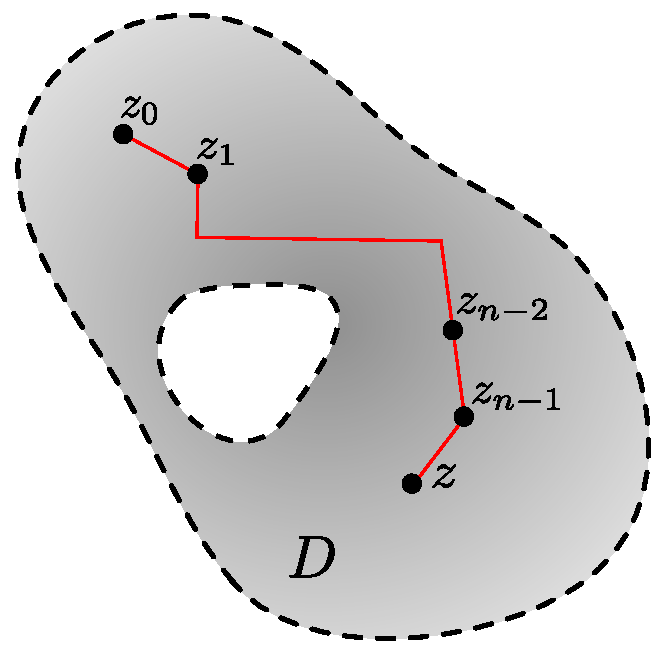
\includegraphics[scale = 0.5]{Figuras/DerivadaNula.pdf}
    \caption{Camino poligonal que une los puntos $z_0$ y $z$ de un abierto conexo $D$.}
    \label{fig:DerivadaNula}
\end{figure}

y, en consecuencia, $u(x_0,y_0) = u(x,y)$. Como $(x,y)$ es arbitrario, hemos probado que $u = cte$ para todo $z \in D$. De forma análoga, se prueba que $v$ es constante en $D$. Por lo tanto, $f$ es constante en $D$.
\end{proof}

\textbf{Observación:} La conexión de $D$ no puede ser omitida en la hipótesis del teorema. Por ejemplo, para el abierto no conexo $D = \{z \in \mathbb{C}: |z| < 2 \vee |z|> 3\}$, la función $f: D \rightarrow \mathbb{C}$ definida por
$$f(z) = \left\{ \begin{array}{cl}
     1,& \mbox{si} ~ |z|  < 2  \\
    0, & \mbox{si} ~ |z|  > 3
\end{array} \right. .$$

tiene derivada nula, pero no es constante.

\section{Funciones inversas*}

Al igual que el caso real, también se tiene un teorema de la función inversa. Antes de enunciar lo recordemos el teorema para variables reales en dos dimensiones:

\begin{teorema}\label{InversaCIII}
Si $f: A \subseteq \mathbb{R}^2 \longrightarrow \mathbb{R}^2$ es continuamente diferenciable en el abierto $A$ y $Jf(x_0,y_0)$ tiene determinante distinto de cero, entonces existen vecindades $U$ de $(x_0,y_0)$ y $V$ de $f(x_0,y_0)$ tales que $f: U \longrightarrow V$ es una biyección, $f^{-1}: V \longrightarrow U$ es diferenciable, y
$$Jf^{-1}(f(x,y)) = [Jf(x,y)]^{-1}.$$
\end{teorema}

\begin{teorema}[de la función inversa]
Sea $f: A \subseteq \mathbb{C} \longrightarrow \mathbb{C}$ analítica (con $f'$ continua) \footnote{Más adelante, por medio del teorema de Cauchy, veremos que  la analiticidad de la función implica directamente la continuidad de $f'$. } y suponga que $f'(z_0) \neq 0$. Entonces existe una vecindad $U$ de $z_0$ y una vecindad $V$ de $f(z_0)$ tal que $f: U \longrightarrow V$ es una biyección y su inversa $f^{-1}$ es analítica con su derivada dada por
$$\frac{d}{dw} f^{-1}(w) = \frac{1}{f'(z)}, \quad \forall w = f(z) \in V.$$
\end{teorema}

\begin{proof}
Por hipótesis, tenemos que $f(z) = (u(x,y), v(x,y)) = u(x,y) + iv(x,y)$ es analítica en $A$, entonces $u$ y $v$ satisfacen las ecuaciones de Cauchy-Riemann. Luego, la matriz Jacobiana está dada por
$$\forall (x,y) \in A: ~ Jf(x,y) = \begin{pmatrix}
\frac{\partial u}{\partial x} & \frac{\partial u}{\partial y} \\
\frac{\partial v}{\partial x} & \frac{\partial v}{\partial y}
\end{pmatrix}  = \begin{pmatrix}
\frac{\partial u}{\partial x} & -\frac{\partial v}{\partial x} \\
\frac{\partial v}{\partial x} & \frac{\partial u}{\partial x}
\end{pmatrix}$$

con determinante
$$\left(\frac{\partial u}{\partial x} \right)^2 + \left(\frac{\partial v}{\partial x} \right)^2 = |f'(z)|^2$$

ya que $f'(z) = u_x + i v_x $.  Ahora para $(x,y) = (x_0,y_0) = z_0$, se tiene que $f'(z_0) \neq 0$, por lo tanto, $|Jf(x_0,y_0)| = |f'(z_0)|^2 \neq 0$. Entonces, por el teorema de la función inversa para variable real, existen vecindades $U$ de $z_0$ y $V$ de $f(z_0)$ tales que $f: U \longrightarrow V$ es biyectiva. 

Basta probar que la inversa $f^{-1}: V \longrightarrow U$ es analítica. Para ello, consideremos la inversa de $Jf$:
$$\frac{1}{|Jf|} \begin{pmatrix} \frac{\partial v}{\partial y} & - \frac{\partial u}{\partial y} \\
-\frac{\partial v}{\partial x} & \frac{\partial u}{\partial x}
\end{pmatrix}.$$

Si escribimos $f^{-1}(x,y) = (t(x,y) , s(x,y)) =  t(x,y) + i s(t,y)$, entonces, comparando
$$J f^{-1} = \begin{pmatrix} \frac{\partial t}{\partial x} &  \frac{\partial t}{\partial y} \\
\frac{\partial s}{\partial x} & \frac{\partial s}{\partial y}
\end{pmatrix}$$

con la matriz inversa de $Jf$, obtenemos
\begin{align*}
    \frac{\partial t}{\partial x} &= \frac{1}{|Jf|} \frac{\partial v}{\partial y} = \frac{1}{|Jf|} \frac{\partial u}{\partial x}, \\
    \frac{\partial s}{\partial x} &= -\frac{1}{|Jf|} \frac{\partial v}{\partial x} = \frac{1}{|Jf|} \frac{\partial u}{\partial y}, \\
     \frac{\partial t}{\partial y} &= -\frac{1}{|Jf|} \frac{\partial u}{\partial y} = \frac{1}{|Jf|} \frac{\partial v}{\partial x}, \\
      \frac{\partial s}{\partial y} &= \frac{1}{|Jf|} \frac{\partial u}{\partial x} = \frac{1}{|Jf|} \frac{\partial v}{\partial y}.
\end{align*}

De esta forma hemos probado que para todo $(x,y) \in V$, se verifica que
\begin{align*}
    t_x &= s_y , \\
    t_y &= - s_x.
\end{align*}

Así las ecuaciones de Cauchy-Riemann se satisfacen para $t$ y $s$ ya que se satisfacen para las funciones continuamente diferenciables $u$ y $v$. Por lo tanto, $f^{-1}$ es analítica. Además, 
$$(f^{-1})'(w) = \frac{\partial t}{\partial x} + i \frac{\partial s}{\partial x} = \frac{1}{|Jf|} \left( \frac{\partial u}{\partial x} - i \frac{\partial v}{\partial x} \right) = \frac{\overline{f'(z_0)}}{|f'(z_0)|^2} = \frac{1}{f'(z_0)}, \quad w = f(z_0).$$
\end{proof}

\textbf{Observación:} El teorema de la función inversa nos garantiza la existencia de una inversa local para $f$. Por ejemplo, si consideramos $f(z) = z^2$ definida en $A = \mathbb{C} \setminus \{0\}$. Entonces $f'(z) = 2z \neq 0$ en cada punto de $A$. El teorema de la función inversa dice que $f$ tiene una inversa analítica local, que es simplemente alguna rama de la función raíz cuadrada. Pero $f$ no es inyectiva en todo $A$, pues, por ejemplo, $f(1) = f(-1)$.

\section{Funciones armónicas}

Recordemos que una función $h(x,y)$ a valores reales con dominio en el plano $xy$ se dice \textbf{armónica} si sobre ese dominio tiene derivadas parciales continuas de primer y segundo orden, y satisfacen la ecuación
$$\nabla^2 h = h_{xx}(x,y) + h_{yy} (x,y) = 0,$$

la cual es conocida como la \textbf{ecuación de Laplace}. Esta ecuación aparece en muchas ramas de la física tales como la astronomía, la electrostática, la mecánica de fluidos o la mecánica cuántica. Por ejemplo, si tenemos un sistema electrostático (cargas en reposo), el campo eléctrico puede ser escrito a partir de un potencial (electrostático) $\phi$ tal que $\Vec{E} = -\nabla \phi$. Reemplazando en la ley de Gauss en su forma diferencial:
$$\nabla \cdot \Vec{E} = \frac{\rho}{\varepsilon} \Rightarrow \nabla \cdot ( - \nabla \phi) = \frac{\rho}{\varepsilon}  \Rightarrow \nabla^2 \phi = -\frac{\rho}{\varepsilon},$$

es decir, el potencial satisface la \textbf{ecuación de Poisson}. Para regiones del espacio libre de fuentes de cargas, ésto es, $\rho \equiv 0$, el potencial satisface la ecuación de Laplace.
\\
 
Asumamos, ahora, que tenemos una función compleja y analítica
$$f(z) = u(x,y) + iv(x,y).$$

La pregunta que nos podemos hacer es si las funciones $u(x,y)$ y $v(x,y)$ son armónicas. La respuesta está en el siguiente teorema, el cual, para su demostración, se asumirá el siguiente resultado que será demostrado más adelante:

\begin{quote}
\textit{Las funciones componentes de una función analítica en un punto admiten derivadas parciales continuas de todos los órdenes en dicho punto.}
\end{quote}

\begin{teorema}
Si $f(z) = u(x,y) + iv(x,y)$ es analítica en un dominio $D$, entonces sus funciones componentes $u$ y $v$ son armónicas en $D$.
\end{teorema}

\begin{proof}
Dado que $f$ es analítica, las funciones componentes satisfacen las ecuaciones de Cauchy-Riemann en su dominio, ésto es,
\begin{eqnarray*}
u_x &=& v_y ,\\
u_y &=& -v_x .
\end{eqnarray*}

Derivando en ambos lados de las ecuaciones con respecto a $x$, tenemos:
\begin{eqnarray*}
u_{xx} &=& v_{yx}, \\
u_{yx} &=& -v_{xx}. 
\end{eqnarray*}

De igual manera, lo hacemos con respecto a $y$:
\begin{eqnarray*}
u_{xy} &=& v_{yy},\\
u_{yy} &=& -v_{xy} .
\end{eqnarray*}

Como las funciones componentes de $f$ tienen derivadas segundas continuas (porque $f$ es analítica), las derivadas cruzadas son iguales. Entonces,
\begin{eqnarray*}
u_{xx} &=& v_{yx} = v_{xy}, \\
u_{yy} &=& - v_{xy} = - v_{yx}, \\
v_{xx} &=& - u_{yx} = - u_{xy}, \\
v_{yy} &=& u_{xy} = u_{yx} .
\end{eqnarray*}

Por lo tanto,
$$u_{xx} + u_{yy} = 0 ~~\mbox{y}~~ v_{xx} + v_{yy} = 0,$$

es decir, $u$ y $v$ son armónicas.

\end{proof}

\begin{defi}
Si dos funciones $u(x,y)$ y $v(x,y)$ son armónicas en un dominio $D$ y sus derivadas parciales satisfacen las ecuaciones de Cauchy-Riemann en $D$; en otras palabras, la función $f = u + iv$ es analítica en $D$. Entonces  $v$ es llamada la \textbf{armónica conjugada} de $u$. 
\end{defi}

Es evidente que si una función $f(z) = u(x,y) + iv(x,y)$ es analítica en un dominio $D$, entonces $v$ es una armónica conjugada de $u$. Recíprocamente, si $v$ es una armónica conjugada de $u$ en un dominio $D$, la función $f$ es analítica en $D$. Ésto es consecuencia del teorema \ref{ECR} . Enunciamos este resultado como teorema.

\begin{teorema}
Una función $f(z) = u(x,y) + iv(x,y)$ es analítica en un dominio $D$ si y sólo si $v$ es una armónica conjugada de $u$.
\end{teorema}

\begin{ejemplo}
Consideremos las siguientes funciones definidas en el plano $xy$:
$$u(x,y) = x^2-y^2, \quad v(x,y) = 2xy.$$

Sus derivadas parciales son:
\begin{eqnarray*}
u_x = 2x; ~ v_y = 2x\\
u_y = -2y; ~ v_x = 2y
\end{eqnarray*}

Así, 
$$u_x = v_y ~~\mbox{y}~~ u_y = -v_x.$$

Pero,
$$v_x = - u_y ~~\mbox{y}~~ v_y = u_x,$$

es decir, no se cumplen las ecuaciones de Cauchy-Riemann. En consecuencia,
$$f(z) = x^2-y^2 + i2xy$$

es analítica en su dominio, entonces $v$ es la armónica conjugada de $u$, en cambio,
$$g(z) = 2xy + i(x^2-y^2)$$

no es analítica en punto alguno de su dominio, luego $u$ no es la armónica conjugada de $v$.
\end{ejemplo}

\begin{propo}

Algunas propiedades de las armónicas conjugadas son:

\begin{enumerate}
\item Si $v$ es armónica conjugada de $u$ y $u$ es armónica conjugada de $v$, entonces ambas funciones $u$ y $v$ son constantes.

\item Si $v$ es armónica conjugada de $u$, entonces $-u$ es armónica conjugada de $v$.

\item La función $f(z) = u(x,y) + iv(x,y)$  es analítica en su dominio si, y sólo si $if(z) = v(x,y) - iu(x,y)$ es analítica en dicho dominio.

\item Si $v$ y $w$ son armónicas conjugadas de $u$, entonces $v = w + C$, $C = cte$.
\end{enumerate}
\end{propo}

\begin{proof}
Queda como ejercicio para el lector.
\end{proof}

\textbf{Observación:} Es posible mostrar que toda función armónica definida en un cierto dominio tiene una armónica conjugada. Para determinarla, veamos el siguiente ejemplo.

\begin{ejemplo}
Sea  la función
$$u(x,y) = y^3-3x^2y.$$

Sus derivadas parciales segundas no cruzadas son:
$$u_{xx} = -6y, \quad u_{yy} = 6y. $$

Luego, $u$ es armónica para todo $(x,y) \in \mathbb{R}^2$. Notemos que si $v = v(x,y)$ es la armónica conjugada, entonces
$$u_x = -6xy = v_y.$$

Así,
$$v(x,y) = \int v_y dy = \int -6xy \,dy = -3xy^2 + C(x).$$

Ahora,
$$v_x = -3y^2 + C'(x) = -u_y = -3y^2 + 3x^2.$$

Entonces,
$$C'(x) = 3x^2 ~\Rightarrow~ C(x) = x^3 + c.$$

De esta manera,
$$v(x,y) = -3xy^2 + x^3 + c$$

es la armónica conjugada de $u$.
\end{ejemplo}

\textbf{Observación:} Por el ejemplo anterior, podemos construir funciones analíticas a partir de una función armónica. En ese caso,
$$f(z) = y^3 - 3x^2y + i(x^3 -3xy^2 + c) = i(z^3+c).$$

Por último, probemos el siguiente resultado:

\begin{quote}
    Dada una función armónica $u(x,y)$ definida sobre un dominio $D$ simplemente conexo\footnote{Un conjunto en el plano es \textit{simplemente conexo} si al tomar curvas cerradas dentro del conjunto, el interior sigue estando en el conjunto. En otras palabras, si el conjunto no posee agujeros.}, $u(x,y)$ admite siempre una armónica conjugada $v(x,y)$ en $D$.
\end{quote}

Recordemos del Cálculo III lo siguiente: Supongamos que $P(x,y)$ y $Q(x,y)$ tienen derivadas parciales de primer orden continuas en un dominio $D$ simplemente conexo del plano $xy$, y sean $(x_0,y_0)$ y $(x,y)$ dos puntos cualesquiera en $D$. Si $P_y = Q_x$ en todo punto de $D$, entonces el campo vectorial $\Vec{F} = (P,Q)$ es conservativo y la integral de línea
$$\int_C P(s,t) ds + Q(s,t) dt$$

desde $(x_0,y_0)$ hasta $(x,y)$, es independiente de la curva $C$ escogida, siempre que esté contenida en $D$. Además, si el punto $(x_0,y_0)$ se mantiene fijo y se permite que $(x,y)$ varíe sobre $D$, la integral representa una función univaluada
$$\phi(x,y) = \int_{(x_0,y_0)}^{(x,y)} P(s,t) ds + Q(s,t) dt$$

de $x$ e $y$ conocida como potencial de $\Vec{F}$, cuyas primeras derivadas parciales vienen dadas por las ecuaciones
\begin{equation}
  \frac{\partial \phi}{\partial x}(x,y) = P(x,y), ~ \frac{\partial \phi}{\partial y}(x,y) = Q(x,y).  \label{ArmoConj1}
\end{equation}

Notemos que el valor de $\phi$ cambia en una constante aditiva cuando se toma un punto $(x_0,y_0)$ diferente.

Volviendo a la función armónica dada $u(x,y)$, observemos que de la ecuación de Laplace $u_{xx} + u_{yy} = 0$ se sigue que
$$(-u_y)_y = (u_x)_x$$

en todo punto de $D$. Asimismo, como las segundas derivadas parciales de $u$ son continuas en $D$, las derivadas de primer orden de $-u_y$ y $u_x$ son continuas ahí. Así pues, si $(x_0,y_0)$ es un punto fijo de $D$, la función
$$v(x,y) = \int_{(x_0,y_0)}^{(x,y)} - u_t(s,t) ds + u_s(s,t) dt$$

está bien definida para todo $(x,y) \in D$, y de acuerdo con \eqref{ArmoConj1},
$$v_x(x,y) = - u_y(x,y),~ v_y(x,y) = u_x(x,y),$$

ésto es, $u$ y $v$ satisfacen las ecuaciones de Cauchy-Riemann. Como las derivadas de primer orden de $u$ son continuas, es evidente que las de $v$ también son continuas. Por tanto, $u+iv$ es una función analítica en $D$, y $v$ es, por consiguiente, una armónica conjugada de $u$. 

Claramente la función $v$ no es la única armónica conjugada de $u$. La función $v(x,y) + c$, con $c\in \mathbb{R}$ es también una armónica conjugada de $u$.
\chapter{Funciones elementales}

\section{Funciones multivaluadas} \label{Multivaluadas}

\subsection{Definiciones}

En cursos anteriores hemos aprendido que una función es una aplicación que a cada elemento del dominio le hace corresponder un único elemento del codominio. En variable compleja también ocurre lo mismo, sin embargo, es conveniente trabajar con aplicaciones que a cada número complejo le asocia un conjunto de números complejos.

\begin{defi}
Sea la función compleja $w = f(z)$, si para cada valor de la variable independiente $z$ existe uno y solo un punto imagen $w$, se dice que la función es \textbf{uniforme} o \textbf{monovaluada} o \textbf{univaluada}. En caso contrario, la función se dice \textbf{multiforme} o \textbf{multivaluada}.
\end{defi}

Por definición, una función es \textbf{multivaluada} si para cada valor de la variable $z$ existen más de un valor de la variable $w$. Los ejemplos más notables que hemos visto hasta ahora son: $arg(z)$ y $z^{1/n}$. La mayoría de las funciones multivaluadas aparecen cuando se intenta determinar la inversa de funciones univaluadas no inyectivas.

\begin{figure}[H]
    \centering
    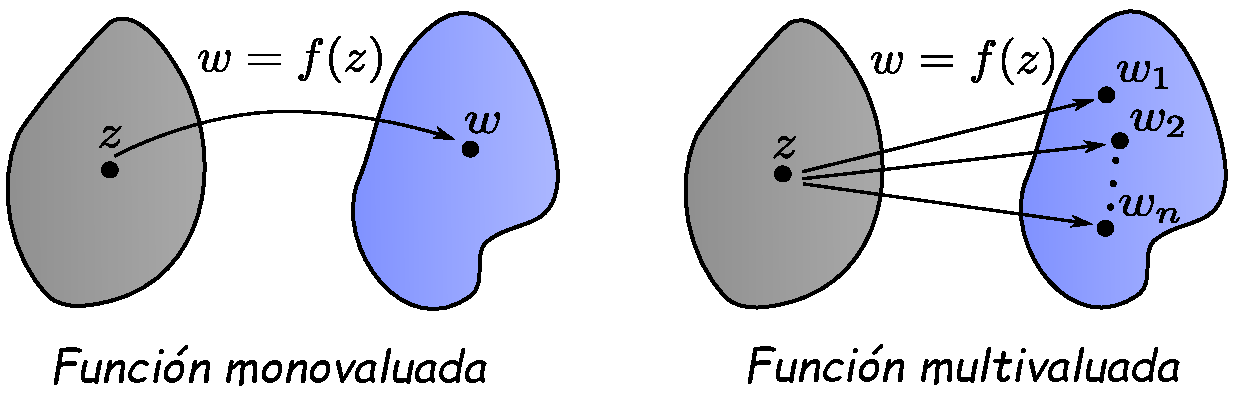
\includegraphics[scale=0.6]{Figuras/Funciones_Multivaluadas.pdf}
    \caption{Función multivaluada.}
    \label{MultiF}
\end{figure}

Para funciones multivaluadas, nos interesará conocer el mayor dominio en donde ésta sea una función monovaluada.

\begin{defi}
Sea $f(z)$ una función multivaluada definida en un dominio $D \subseteq \mathbb{C}$. Diremos que $F(z)$ es una \textbf{rama} o \textbf{determinación continua} de $f(z)$ en $D$ si:
\begin{enumerate}
    \item $F(z)$ es una función monovaluada.
    
    \item $F(z)$ es uno de los posibles valores de $f(z)$ para cada $z \in D$.
    
    \item $F$ es continua en $D$.
\end{enumerate}
\end{defi}

\begin{ejemplo}
Recordemos que si se restringe el argumento de un complejo a $- \pi < \theta \leq \pi$, obtenemos el argumento principal $Arg(z)$. La función $f(z) = Arg(z)$ es monovaluada y continua en $\mathbb{C} \setminus \,]- \infty,0]$ y en el semieje real negativo presenta una discontinuidad de salto. En otras palabras,  $Arg(z)$ es una \textit{rama} de la función multivaluada $arg(z)$ en $\mathbb{C} \setminus \,]- \infty,0]$.
\end{ejemplo}

\begin{ejemplo}
Sabemos que la raíces cúbicas de un número complejo $z = r e^{i \theta}$ están dadas por 
$$\sqrt[3]{r} \exp \left( i \frac{\theta + 2k\pi}{3} \right), \quad k = 0,1,2.$$

Por lo tanto, para cada $k$ se obtienen las tres ramas de la función $w = f(z) = z^{1/3}$:
\begin{align*}
w_1 &= |z|^{1/3} e^{i\theta/3}  \\
w_2 &= |z|^{1/3} e^{i(\theta/3 + 2\pi/3)}  \\
w_3 &= |z|^{1/3} e^{i(\theta/3 + 4\pi/3)}    
\end{align*}

donde $0 < \theta < 2\pi$. 

Notemos que los $z \in \mathbb{C}$ tales que $\theta = 0, 2\pi$ se omiten, pues la rama dejaría de ser continua.
\end{ejemplo}

\subsection{Ramas y puntos de ramificación}

En esta subsección profundizaremos el concepto de rama de una función multivaluada, para ello comencemos con un ejemplo.

\begin{ejemplo} \label{EjemploRaiz}
Consideremos la función $w = f(z) = \sqrt{z}$. Si $z = r e^{i\theta}$ las raíces cuadradas están dadas por
$$\sqrt{r} \exp \left(\frac{\theta + 2k\pi}{2} \right), \quad k = 0,1.$$

Entonces, para cada $k$ se obtienen las dos ramas de la función:
\begin{align*}
    w_1 &= \sqrt{r} e^{i \theta/2}, \\
    w_2 &= \sqrt{r} e^{i (\theta/2 + \pi)} = -w_1.
\end{align*}

Para $\theta \in ]0, 2\pi[$, grafiquemos las ramas de la función, ver figura \ref{fig:Raiz1}. Notemos que omitimos los extremos $\theta = 0,2\pi$ y el origen, es decir, el conjunto
\begin{equation}
\{ z \in \mathbb{C} : Re(z) \geq 0 \wedge Im(z) = 0\},    \label{CorteRama1}
\end{equation}

porque la rama dejaría de ser continua. Observemos que la curva que separa ambas ramas es el eje real, la cual correspondería al evaluar $f$ en \eqref{CorteRama1}. Debido a ésto este conjunto es conocido como \textit{corte de ramificación}.

\begin{figure}[H]
    \centering
    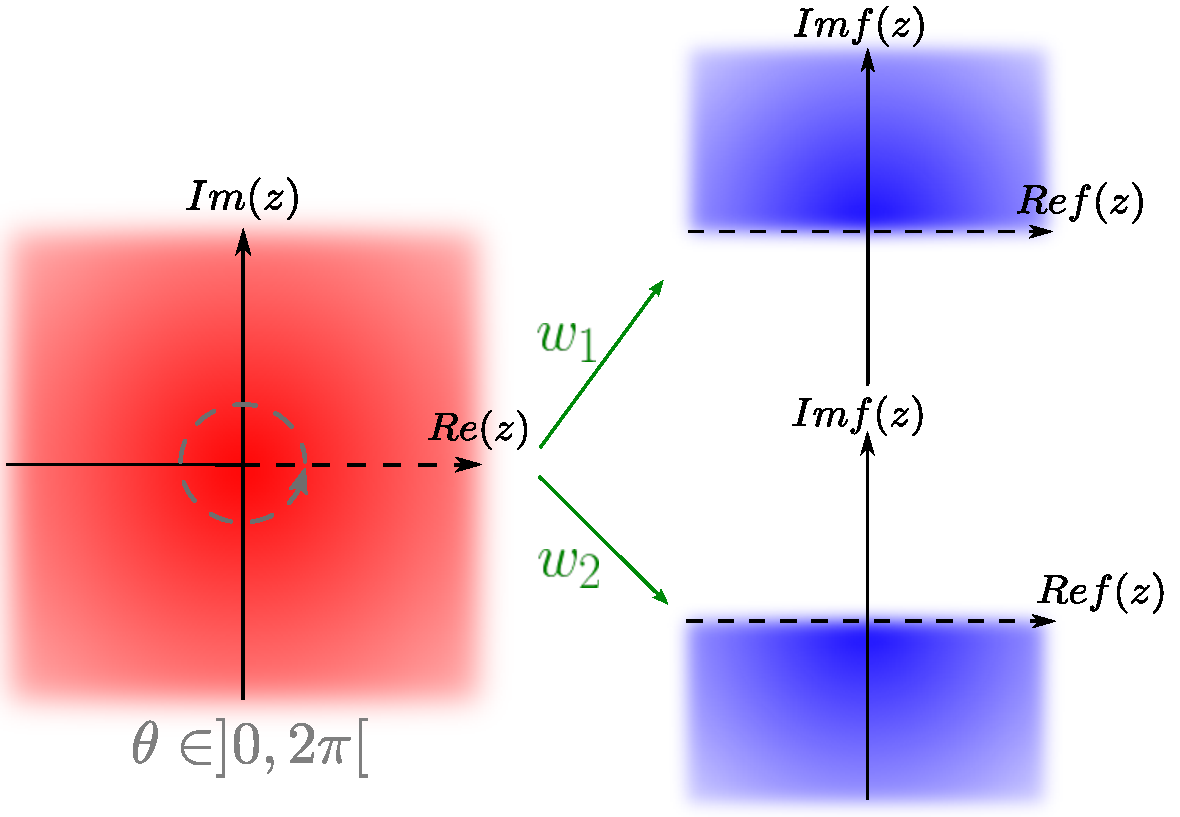
\includegraphics[scale = 0.5]{Figuras/RaizCuadrada1.pdf}
    \caption{Gráficas de las ramas de la función raíz cuadrada $f(z) = \sqrt{z}$ para $z = r e^{i\theta}$ con $\theta \in ]0,2\pi[$.}
    \label{fig:Raiz1}
\end{figure}

¿Qué pasaría si consideramos otro intervalo de longitud $2\pi$ como $]-\pi, \pi[$?
\\

Para $\theta \in ]-\pi, \pi[$, las gráficas de las ramas de la función están representadas en la figura \ref{fig:Raiz2}. En este caso, el corte de ramificación corresponde al conjunto 
\begin{equation}
\{ z \in \mathbb{C} : Re(z) \leq 0 \wedge Im(z) = 0\},    \label{CorteRama2}
\end{equation}

\begin{figure}[H]
    \centering
    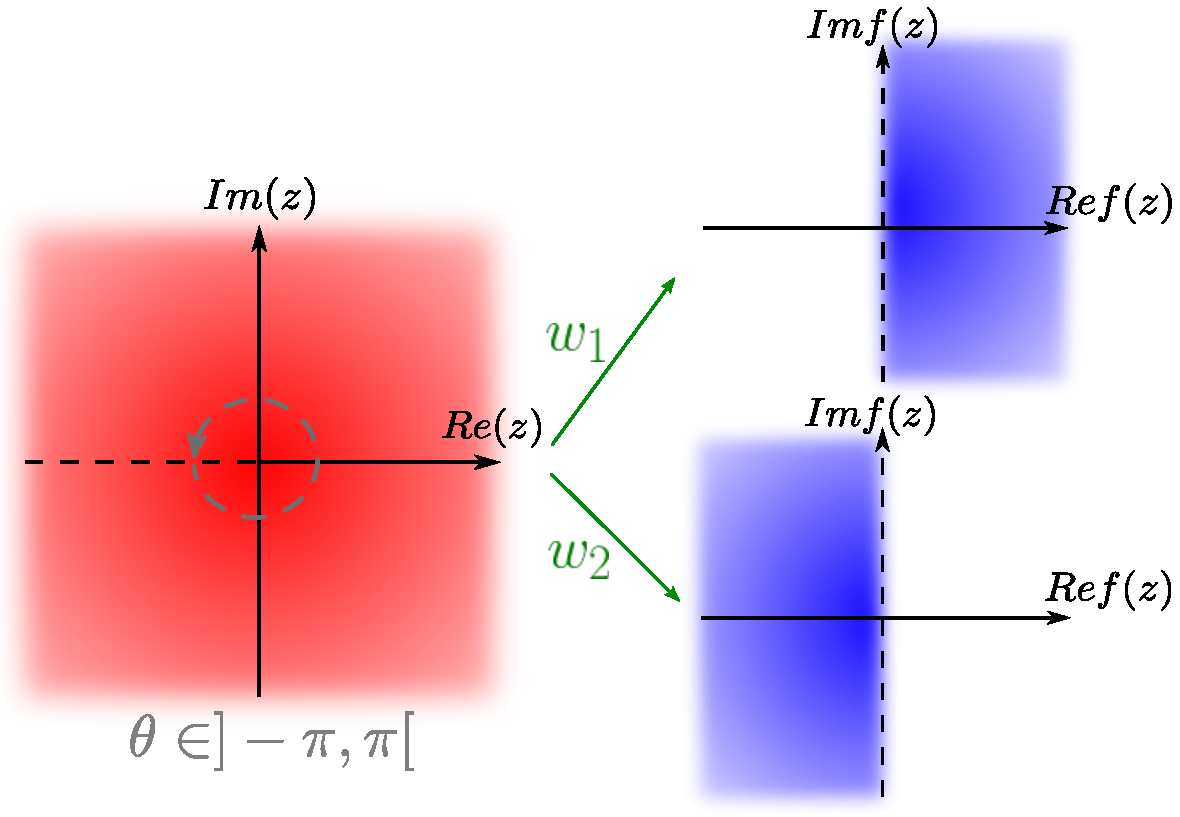
\includegraphics[scale = 0.5]{Figuras/RaizCuadrada2.pdf}
    \caption{Gráficas de las ramas de la función raíz cuadrada $f(z) = \sqrt{z}$ para $z = r e^{i\theta}$ con $\theta \in ]-\pi,\pi[$.}
    \label{fig:Raiz2}
\end{figure}

\end{ejemplo}

\begin{defi}
Un \textbf{corte de ramificación} es una línea (habitualmente recta) que separa dos ramas de una misma función multivaluada. Equivalentemente, es la línea en la que una rama se hace discontinua.
\end{defi}

\begin{defi}
Sea $f(z)$ una función multivaluada y $z_0$ un punto de su dominio. Decimos que $z_0$ es un \textbf{punto de ramificación} de $f(z)$ si una vuelta alrededor de $z_0$ (y suficientemente cerca a $z_0$) produce un cambio de rama de la función. 
\end{defi}

\begin{ejemplo}
El complejo $z = 0$ es un punto de ramificación de $f(z) = \sqrt{z}$.
\end{ejemplo}

\textbf{Observación:} Los cortes de ramificación son curvas por las que hacemos discontinuas las ramas y que impiden que podamos dar una vuelta completa alrededor de un punto de ramificación. Como pudimos notar en el ejemplo \ref{EjemploRaiz}, los cortes de ramificación no son únicos y podemos elegirlos según nos convenga.

Así cada punto de ramificación deben tener en común todos los cortes de $f$.

\section{Función exponencial}

\begin{defi}
Llamaremos \textbf{función exponencial} a $f: \mathbb{C} \longrightarrow \mathbb{C}$ tal que
$$f(z) = e^x(\cos y + i \sin y),$$

la cual denotamos por $e^z = \exp(z)$.
\end{defi}

\begin{propo}
\ 

\begin{enumerate}
    \item La función exponencial $f(z) = e^z$ es entera y $f'(z) = f(z)$.
    
    \item La función exponencial es la única función que cumple $f'(z) = f(z)$ con $f$ entera y $f(x + i0) = e^x$ (se recupera la exponencial real).
\end{enumerate}
\end{propo}

\begin{proof}
\ 

\begin{enumerate}
    \item Las funciones componentes de $e^z$ son
$$u(x,y) = e^x \cos y; \quad v(x,y) = e^x \sin y.$$

Además, 
\begin{align*}
u_x &= e^x \cos y = v_y, \\
u_y &= -e^x \sin y = -v_x,
\end{align*}

es decir, $f$ es una función \underline{entera} y 
\begin{equation*}
f'(z) = f(z) ~~\mbox{o}~~ \frac{d}{dz}(e^z) = \frac{d}{dz}(\exp(z)) = e^z.
\end{equation*}

\item Supongamos que la función $f(z) = u(x,y) + i v(x,y)$ es una función entera con $f'(z) = f(z)$, luego ésta satisface las ecuaciones de Cauchy-Riemann y 
$$f'(z) = u_x(x,y) + i v_x(x,y) = u(x,y) + iv(x,y) ~\Rightarrow~ \left\{ \begin{array}{ccc}
u_x(x,y) &=& u(x,y) \\
v_x(x,y) &=& v(x,y) 
\end{array} \right. .$$

De la primera ecuación, tenemos que
\begin{align*}
u_x (x,y) - u(x,y) = 0 \quad \color{red}{/\cdot e^{-x}} &\Rightarrow e^{-x} u_x (x,y) - e^{-x} u(x,y) = 0 \\
&\Rightarrow \frac{\partial}{\partial x} \left[ u(x,y)e^{-x} \right] = 0 \\
&\Rightarrow  u(x,y)e^{-x} = \phi(y) \\
&\Rightarrow  u(x,y) = e^{x} \phi(y).
\end{align*}

Análogamente se prueba que 
$$v(x,y) = e^x \psi(y).$$

Ahora, que $f$ sea entera nos dice también que sus componentes son funciones armónicas, en particular se cumple 
\begin{equation*}
u_{xx}(x,y) + u_{yy}(x,y) = 0 ~\Rightarrow~ e^x \phi(y) + e^x \phi''(y) = 0 ~\Rightarrow ~\phi''(y) + \phi(y) = 0.
\end{equation*} 

La EDO de segundo orden homogénea tiene como solución
$$\phi(y) = A \sin y + B \cos y,$$

con $A$ y $B$ constantes de integración.

Ahora, si hacemos lo mismo para $\psi(y)$ obtendríamos otras constantes de integración que a priori no tienen porqué ser iguales a las de $\phi$, sin embargo, de la ecuación de Cauchy-Riemann, $u_y = -v_x$ se tiene que
\begin{equation*}
e^x \phi'(y) = -e^x \psi(y) ~\Rightarrow~ \psi(y) = -A \cos y + B \sin y.
\end{equation*}

Si además añadimos la condición que  
$$f(x+i0) = u(x,0) + i v(x,0) = e^x,$$

obtenemos 
$$e^x (B - iA) = e^x ~\Rightarrow~ B = 1 + iA.$$

Entonces,
$$f(z) = u(x,y) + i v(x,y) = e^x ((B-iA) \cos y + (A + iB)\sin y) = e^x (\cos y + i \sin y).$$
\end{enumerate}
\end{proof}



La forma más compacta 
$$e^z = e^xe^{iy}$$

de la exponencial permite demostrar la siguiente proposición.

\begin{propo}[Propiedades de la exponencial]
Sean $z_1, z_2 \in \mathbb{C}$, se verifica: 

\begin{enumerate}
\item $\exp(z_1 + z_2) = \exp(z_1) \exp(z_2)$.

\item $\frac{\exp(z_1)}{\exp(z_2)} = \exp(z_1 - z_2)$.

\item $e^0= 1; ~ 1/e^z = e^{-z}; ~ (e^z)^n = e^{nz}, \quad n \in \mathbb{Z}.$
\end{enumerate}
\end{propo}

\begin{proof}
Sean $z_1 = x_1 + iy_1$, $z_2 = x_2 + iy_2$ números complejos cualesquiera. 

\begin{enumerate}
\item 
\begin{align*}
\exp(z_1 + z_2) = \exp((x_1+x_2) + i (y_1+y_2)) &= e^{x_1 + x_2} e^{i(y_1+y_2)} \\
&=  [e^{x_1}e^{x_2}][e^{iy_1} e^{iy_2}] \\
&= [e^{x_1} e^{iy_1}][e^{x_2} e^{iy_2}] \\
 &= \exp(z_1) \exp(z_2).
\end{align*}

\item 
\begin{align*}
\frac{\exp(z_1)}{\exp(z_2)} = \frac{\exp(x_1 + iy_1)}{\exp(x_2+iy_2)} &= \frac{e^{x_1} e^{iy_1}}{e^{x_2} e^{iy_2} } \\
&=  \left[\frac{e^{x_1}}{e^{x_2}}\right]\left[\frac{e^{iy_1}}{e^{iy_2}}\right] \\
&= e^{x_1-x_2} e^{i(y_1-y_2)} \\
&= \exp(z_1-z_2).
\end{align*}

\item Es fácil de ver que $e^0 = e^{0+i0} = 1$, luego 
$$\frac{1}{e^{z}} = \frac{e^0}{e^{z}} = e^{-z}.$$

Probemos por inducción que $(e^{z})^n = e^{nz}$, $n \in \mathbb{Z}$.

Para $n = 0,1$; $(e^{z})^0 = 1 = e^{0\cdot z}$ y $e^z = e^{1\cdot z}$. 

Suponiendo que para $n \in \mathbb{N}$ se verifica 
$$(e^{z})^n = e^{nz},$$

tenemos que 
$$(e^{z})^{n+1} = (e^{z})^n e^z = e^{nz} e^z = e^{(n+1)z}.$$

Por lo tanto, 
$$(e^{z})^n = e^{nz}; \quad n = 0,1,2, \dots$$

Ahora, haciendo $m = -n$ con $n \in \mathbb{N}$, resulta que 
$$(e^z)^m = (e^z)^{-n} = ((e^{z})^{-1})^n = \left(\frac{1}{e^z}\right)^n = (e^{-z})^n = e^{-nz} = e^{mz}. $$

Finalmente, hemos probado que 
$$(e^{z})^n = e^{nz}, \quad n \in \mathbb{Z}.$$

\end{enumerate}
\end{proof}

Veamos ahora más propiedades de la función exponencial

\newpage
\begin{propo}
\ 

\begin{enumerate}
    \item El recorrido de la función exponencial es $\mathbb{C} \setminus \{0\}$.
    
    \item $e^z$ no es inyectiva, es más, tiene periodo $2\pi i$.
\end{enumerate}
\end{propo}

\begin{proof}
\ 

\begin{enumerate}
    \item Escribamos $\exp(z)$ como 
$$e^z = \rho(\cos\phi + i \sin\phi)$$

donde $\rho = e^x$ y $\phi = y$. Así, 
$$|e^z| = e^x > 0; ~ arg(e^z) = y + 2n\pi, \quad n \in \mathbb{Z}.$$

Nótese que al ser $|e^z|$ siempre positivo, 
$$\forall z \in \mathbb{C}: ~w = e^z \neq 0.$$

Por otro lado, sea
$$w = r (\cos\theta + i \sin \theta), \quad r >0$$

un complejo distinto de cero. Se define el complejo 
$$z = \ln r + i\theta.$$

Calculemos 
$$e^z = e^{\ln r + i\theta} = e^{\ln r} e^{i\theta} = r (\cos \theta + i\sin\theta) = w.$$

Por lo tanto, todo punto $w$ en el plano complejo menos el origen, es imagen de un $z \in \mathbb{C}$, o sea,
$$Rec(e^z) = \mathbb{C} - \{0\}.$$

\item Ahora como 
\begin{align*}
\cos\theta &= \cos(\theta + 2\pi k ) \\
\sin\theta &= \sin(\theta + 2\pi k)
\end{align*}

con $k \in \mathbb{Z}$, se tiene que la función exponencial \underline{no es inyectiva}, más aún,
$$e^{z + 2\pi i} = e^z,$$

es decir, es \underline{periódica} de periodo $2\pi i$.
\end{enumerate}
\end{proof}

\textbf{Observación:} Si restringimos el dominio de $w = e^z$ a la franja
$$-\pi < Im(z) \leq \pi,$$

la función $w = e^z$ resulta ser inyectiva en esta franja.

Si 
$$w = r (\cos \Phi + i \sin\Phi),$$

donde $Arg(w) = \Phi$, entonces 
$$z = \ln r + i\Phi$$

es tal que 
$$e^{\ln r + i \Phi} = w.$$

\section{Funciones trigonométricas}

\begin{defi}
Llamaremos \textbf{funciones trigonométricas} a las siguientes funciones:
\begin{align*}
\sin z = \frac{e^{iz} - e^{-iz}}{2i} &\qquad \cos z = \frac{e^{iz} + e^{-iz}}{2} \\
\tan z = \frac{\sin z}{\cos z}; ~ \cos z\neq 0 &\qquad \cot z = \frac{\cos z}{\sin z};~\sin z \neq 0 \\
\sec z = \frac{1}{\cos z}; ~ \cos z \neq 0 &\qquad \csc z = \frac{1}{\sin z}; ~ \sin z \neq 0
\end{align*}
\end{defi}

\textbf{Observación:} Es directo de la definición que
$$e^{iz} = \cos z + i \sin z, \quad \forall z \in \mathbb{C}$$

y $\sin^2 z + \cos^2 z = 1$. En efecto,
\begin{align*}
    \sin^2 z + \cos^2 z  &= -\frac{(e^{iz} - e^{-iz})^2}{4} + \frac{(e^{iz} + e^{-iz})^2}{4} \\
    &= \frac{- e^{2iz} + 2 -  e^{-2iz} + e^{2iz} +2 +e^{-2iz}}{4} = 1.
\end{align*}

Determinemos sus derivadas:
\begin{align*}
\frac{d}{dz}[\sin z] &= \frac{1}{2i} [i e^{iz} + i e^{-iz}] = \frac{e^{iz} + e^{-iz}}{2} = \cos z, \\
\frac{d}{dz}[\cos z] &= \frac{1}{2} [i e^{iz} - i e^{-iz}] = - \frac{e^{iz} - e^{-iz}}{2i} = - \sin z, \\
\frac{d}{dz}[\tan z] &= \frac{\cos^2 z + \sin^2 z}{\cos^2 z} = \frac{1}{\cos^2 z} = \sec^2 z, \\
\frac{d}{dz} [\cot z] &= \frac{-\sin^2 z - \cos^2 z}{\sin^2 z} = -\frac{1}{\sin^2 z} = -\csc^2 z, \\
\frac{d}{dz}[\sec z] &= \frac{\sin z}{\cos^2 z} = \frac{1}{\cos z} \frac{\sin z}{\cos z}  = \sec z \tan z, \\
 \frac{d}{dz}[\csc z] &= - \frac{\cos z}{\sin^2 z} = -\frac{1}{\sin z} \frac{\cos z}{\sin z}  = -\csc z \cot z.
\end{align*}

Luego, podemos concluir que las funciones seno y coseno son enteras y las demás analíticas en su dominio de definición.

Note que las derivadas son las mismas que en el caso real, pero ¿conservarán más propiedades de las funciones trigonométricas reales?, por ejemplo, ¿la paridad?
\begin{align*}
\forall z \in \mathbb{C}:~ \sin(-z) &= \frac{e^{-iz} - e^{iz}}{2i} = - \frac{ e^{iz} - e^{-iz} }{2i} = - \sin z , \\
\cos(-z) &= \frac{e^{-iz} + e^{iz}}{2} =  \cos z.
\end{align*}

Entonces, la función seno compleja también es impar y la función coseno compleja es par. De la misma forma se puede probar que la tangente, la cotangente y la cosecante complejas son impares, y la secante compleja es par.

\begin{ejemplo}\label{PropiedadesTrigo}
Muestre que 

\begin{enumerate}
\item $\sin z = \sin x \cosh y + i \cos x \sinh y$.

\item $\cos z = \cos x \cosh y - i \sin x \sinh y$.

\item $\sin(iy) = i \sinh y$; $\cos(iy) = \cosh y$. 

\item $\sin(\overline{z}) = \overline{\sin z}$; $\cos(\overline{z}) = \overline{\cos z}$.
\end{enumerate}

\textbf{Solución:} Sea $z = x + iy \in \mathbb{C}$.

\begin{enumerate}
\item 
\begin{align*}
\sin z =\frac{e^{i(x+iy)} - e^{-i(x+iy)}}{2i} &= \frac{e^{-y + ix} - e^{y - ix}}{2i} \\
&= \frac{e^{-y} e^{ix} - e^{y} e^{-ix}}{2i} \\
&= \frac{e^{-y}(\cos x + i \sin x) - e^y (\cos x - i \sin x)}{2i} \qquad \mbox{(Identidad de Euler)}\\
&= \frac{\cos x (e^{-y} - e^y) + i \sin x (e^{-y} + e^y)}{2i} \cdot \frac{i}{i} \\
&= \sin x \frac{e^y + e^{-y}}{2} + i \cos x \frac{e^y-e^{-y}}{2} \\
&= \sin x \cosh y + i \cos x \sinh y.
\end{align*}

\item 
\begin{align*}
\cos z =\frac{e^{i(x+iy)} + e^{-i(x+iy)}}{2i} &= \frac{e^{-y + ix} + e^{y - ix}}{2} \\
&= \frac{e^{-y} e^{ix} + e^{y} e^{-ix}}{2} \\
&= \frac{e^{-y}(\cos x + i \sin x) + e^y (\cos x - i \sin x)}{2} \qquad \mbox{(Identidad de Euler)}\\
&= \cos x \frac{e^y + e^{-y}}{2} - i \sin x \frac{e^y-e^{-y}}{2} \\
&= \cos x \cosh y - i \sin x \sinh y.
\end{align*}

\item Usando lo demostrado en 1. y 2., tenemos que
\begin{align*}
\sin(iy) &= \sin(0) \cosh y + i \cos(0) \sinh y = i \sinh y, \\
\cos(iy) &= \cos(0) \cosh y - i \sin (0) \sinh y = \cosh y.
\end{align*}

\item Usando lo demostrado en 1., 2. y la paridad de las funciones hiperbólicas reales, tenemos que
\begin{align*}
\sin( \overline{z}) = \sin(x-iy) &= \sin x \cosh(-y) + i \cos x \sinh(-y) \\
&= \sin x \cosh(y) - i \cos x \sinh(y) \\
&= \overline{\sin x \cosh(y) + i \cos x \sinh(y)} \\
&= \overline{\sin z}, \\
\cos( \overline{z}) = \cos(x-iy) &= \cos x \cosh(-y) - i \sin x \sinh(-y) \\
&= \cos x \cosh(y) + i \sin x \sinh(y) \\
&= \overline{\cos x \cosh(y) - i \sin x \sinh(y)} \\
&= \overline{\cos z}.
\end{align*}
\end{enumerate}
\end{ejemplo}

\begin{ejemplo}
Muestre que las funciones trigonométricas son periódicas.
\\

\textbf{Solución:} Para todo $z = x+iy \in \mathbb{C}$, se tiene que 
\begin{align*}
\sin(z + 2\pi) &= \sin(x + 2\pi) \cosh y + i \cos(x + 2\pi) \sinh y = \sin x \cosh y + i \cos x \sinh y = \sin z. \\
\cos(z + 2\pi) &= \cos(x+2\pi) \cosh y - i \sin(x+2\pi) \sinh y = \cos x \cosh y - i \sin x \sinh y = \cos z
\end{align*}

Por lo tanto, la función seno y coseno son periódicas de periodo $2\pi$, de la misma forma se puede probar la misma periocidad para la secante y la cosecante. 

Con respecto a las funciones trigonométricas restantes, observemos que 
\begin{align*}
\tan(z + \pi) &= \frac{\sin(x + \pi) \cosh y + i \cos(x + \pi) \sinh y}{\cos(x+\pi) \cosh y - i \sin(x+\pi) \sinh y} = \frac{-(\sin x \cosh y + i \cos x \sinh y)}{-(\cos x\cosh y - i \sin x \sinh y)} = \tan z. \\
\cot(z + \pi) &= (\tan(z+\pi))^{-1} = (\tan z)^{-1} = \cot z,
\end{align*}

ésto es, la tangente y cotangente son periódicas de periodo $\pi$.

\end{ejemplo}

\begin{ejemplo}
Muestre que 
$$|\sin z|^2 = \sin^2 x + \sinh^2 y; ~ |\cos z|^2 = \cos^2x + \sinh^2y.$$

\textbf{Solución:} Usando lo demostrado en el ejemplo \ref{PropiedadesTrigo}, obtenemos que 
\begin{align*}
|\sin z|^2 &= \sin^2 x \cosh^2 y + \cos^2x \sinh^2 y  = \sin^2 x \cosh^2 y + \sinh^2 y - \sin^2 x \sinh^2 y =  \sin^2x + \sinh^2 y. \\
|\cos z|^2 &= \cos^2 x \cosh^2 y + \sin^2 x \sinh^2 y = \cos^2 x \cosh^2 y + \sinh^2 y - \cos^2 x \sinh^2 y = \cos^2 x + \sinh^2 y.
\end{align*}
\end{ejemplo}

\begin{ejemplo}
Encontrar las fórmulas para 
$$\sin(z_1 + z_2); ~ \cos(z_1+z_2); ~ \sin(2z);~ \cos(2z).$$

\textbf{Solución:} A partir de las propiedades de la exponencial, tenemos 
\begin{align*}
\sin(z_1 + z_2) &= \frac{e^{i(z_1 + z_2)} - e^{-i(z_1 + z_2)}}{2i} \\
&= \frac{e^{iz_1}e^{iz_2} - e^{-iz_1}e^{-iz_2} + e^{iz_1}e^{-iz_2} - e^{iz_1}e^{-iz_2} + e^{-iz_1}e^{iz_2} - e^{-iz_1}e^{iz_2} }{2i}  \\
&= \frac{(e^{iz_1} - e^{-iz_1})(e^{iz_2} + e^{-iz_2}) -e^{iz_1}e^{-iz_2} + e^{-iz_1}e^{iz_2}}{2i} \\
&= \frac{4i \sin z_1 \cos z_2 - (e^{i(z_1 - z_2)} - e^{-i(z_1 - z_2)}) }{2i} \\
&= 2\sin z_1 \cos z_2 - \sin(z_1 - z_2).
\end{align*}

Luego, 
\begin{align*}
2 \sin z_1 \cos z_2 = \sin(z_1 + z_2) + \sin(z_1 - z_2) ~\Rightarrow~ 2 \sin z_2 \cos z_1 &= \sin(z_2 + z_1) + \sin(z_2 - z_1) \\
&= \sin(z_1 + z_2) - \sin(z_1 - z_2).
\end{align*}

Sumando ambas expresiones:
$$\boxed{\sin(z_1 + z_2) = \sin z_1 \cos z_2 +\cos z_1 \sin z_2}$$ 

A partir de esta expresión es fácil de ver que
\begin{equation*}
\sin(2z) = 2 \sin z \cos z, \quad
\sin\left(z + \frac{\pi}{2} \right) = \cos z, \quad 
\cos\left( z + \frac{\pi}{2} \right) = - \sin z.
\end{equation*}

Entonces, 
\begin{align*}
\cos(z_1 + z_2) = \sin\left(z_1 + z_2 + \frac{\pi}{2} \right) &= \sin z_1 \cos\left( z_2 + \frac{\pi}{2} \right) + \cos z_1 \sin\left(z_2 + \frac{\pi}{2} \right) \\
&=  - \sin z_1 \sin z_2 + \cos z_1 \cos z_2.
\end{align*}

Por lo tanto,
$$\boxed{\cos(z_1 + z_2) =  \cos z_1 \cos z_2 - \sin z_1 \sin z_2}$$

En particular,
$$\cos(2z) = \cos^2 z - \sin^2 z.$$
\end{ejemplo}

\begin{ejemplo}
Resuelva las ecuaciones 
$$\sin z = 0; \quad \cos z = 0.$$

\textbf{Solución:} Sea $z = x+iy \in \mathbb{C}$, tenemos que
\begin{align*}
\sin z = 0 ~\Leftrightarrow~ |\sin z|^2 = 0 &\Leftrightarrow \sin^2 x + \sinh^2 y = 0 \\
&\Leftrightarrow~ \sin^2 x = 0 ~\wedge~ \sinh^2 y = 0 \\
 &\Leftrightarrow~  x = n\pi, ~ n \in \mathbb{Z} ~\wedge~ y = 0.
\end{align*}
$$\therefore ~ \sin z = 0 ~\Leftrightarrow~ z = n\pi, \quad n \in \mathbb{Z}.$$

De forma similar, se prueba que 
$$\cos z = 0 ~\Leftrightarrow~ z = \frac{\pi}{2} + n \pi, \quad n \in \mathbb{Z}.$$ 

\end{ejemplo}

De lo anterior, podemos concluir que
\begin{align*}
Dom(\tan z)= Dom(\sec z) &= \left\{z \in \mathbb{C}: z \neq \frac{\pi}{2} + n \pi, ~ n \in \mathbb{Z}  \right\}.\\
Dom(\cot z) = Dom( \csc z) &= \{z \in \mathbb{C}: z \neq n\pi, ~ n \in \mathbb{Z} \}.
\end{align*}

\section{Funciones hiperbólicas}

Las definiciones de las funciones hiperbólicas complejas no difieren de las mismas en el caso real.

\begin{defi}
Llamaremos \textbf{funciones hiperbólicas} a 
\begin{equation*}
\sinh z = \frac{e^z-e^{-z}}{2}; \quad \cosh z = \frac{e^z + e^{-z}}{2}; \quad \tanh z = \frac{\sinh z}{\cosh z}.
\end{equation*}
\end{defi}

Determinemos sus derivadas:
\begin{align*}
\frac{d}{dz}[\sinh z] &= \frac{e^z + e^{-z}}{2} = \cosh z, \\
\frac{d}{dz} [\cosh z] &= \frac{e^z - e^{-z}}{2} = \sinh z, \\
\frac{d}{dz} [\tanh z] &=  \frac{d}{dz}\left[ \frac{e^z - e^{-z}}{e^z + e^{-z}} \right] =  \frac{(e^z + e^{-z})^2 - (e^z - e^{-z})^2}{(e^z + e^{-z})^2} = \frac{4}{(e^z + e^{-z})^2} = \frac{1}{\cosh^2 z}.
\end{align*}

Entonces, la funciones $\sinh z$, $\cosh z$ son enteras y $\tanh z$ analítica en su dominio de definición.
\\

Analicemos la paridad de las funciones hiperbólicas complejas:
\begin{align*}
\forall z \in \mathbb{C}:~ \sinh(-z) &= \frac{e^{-z} - e^{z}}{2} = - \frac{ e^{z} - e^{-z} }{2} = - \sinh z , \\
\cosh(-z) &= \frac{e^{-z} + e^{z}}{2} =  \cosh z.
\end{align*}

Entonces, la función $\sinh$  es impar y la función $\cosh$ es par. De la misma forma se puede probar que $\tanh z$ es impar.

\begin{ejemplo}\label{PropiedadesHiper}
Muestre que 

\begin{enumerate}
\item $\sinh z = \sinh x \cos y + i \cosh x \sin y$.

\item $\cosh z = \cosh x \cos y + i \sinh x \sin y$.

\item $\sinh(iz) = i \sin z$; $\cosh(iz) = \cos z$. 
\end{enumerate}

\textbf{Solución:} Sea $z = x + iy \in \mathbb{C}$.

\begin{enumerate}
\item 
\begin{align*}
\sinh z =\frac{e^{x+iy} - e^{-x-iy}}{2} 
&= \frac{e^{x} e^{iy} - e^{-x} e^{-iy}}{2} \\
&= \frac{e^{x}(\cos y + i \sin y) - e^{-x} (\cos y - i \sin y)}{2} \qquad \mbox{(Identidad de Euler)}\\
&= \frac{\cos y (e^{x} - e^{-x}) + i \sin y (e^{x} + e^{-x})}{2} \\
&=  \frac{e^x - e^{-x}}{2} \cos y + i  \frac{e^x+e^{-x}}{2} \sin y \\
&= \sinh x \cos y + i \cosh x \sin y.
\end{align*}

\item 
\begin{align*}
\cosh z =\frac{e^{x+iy} + e^{-x-iy}}{2} 
&= \frac{e^{x} e^{iy} + e^{-x} e^{-iy}}{2} \\
&= \frac{e^{x}(\cos y + i \sin y) + e^{-x} (\cos y - i \sin y)}{2} \qquad \mbox{(Identidad de Euler)}\\
&= \frac{\cos y (e^{x} + e^{-x}) + i \sin y (e^{x} - e^{-x})}{2} \\
&=  \frac{e^x + e^{-x}}{2} \cos y + i  \frac{e^x-e^{-x}}{2} \sin y \\
&= \cosh x \cos y + i \sinh x \sin y.
\end{align*}

\item Es directo de la definición que
\begin{align*}
\sinh(iz) &= \frac{e^{iz} - e^{-iz}}{2} = i \frac{e^{iz} - e^{-iz}}{2i} = i \sin z, \\
\cosh(iz) &= \frac{e^{iz} + e^{-iz}}{2} = \cos z.
\end{align*}

\end{enumerate}
\end{ejemplo}

\begin{ejemplo}
Muestre que las funciones hiperbólicas son periódicas.
\\

\textbf{Solución:} Para todo $z = x+iy \in \mathbb{C}$, se tiene que 
\begin{align*}
\sinh(z + 2\pi i ) &= \sinh x \cos(y+ 2\pi) + i \cosh x \sin(y + 2\pi) = \sinh x \cos y + i \cosh x \sin y = \sinh z .\\
\cosh(z + 2\pi i) &= \cosh x \cos(y+ 2\pi) + i \sinh x \sin(y+ 2\pi) = \cosh x \cos y + i \sinh x \sin y = \cosh z.
\end{align*}

Por lo tanto, las funciones $\sinh$ y $\cosh$ son periódicas de periodo $2\pi i$.

Por otro lado, 
\begin{equation*}
\tanh(z + \pi i) = \frac{\sinh x \cos(y+ \pi) + i \cosh x \sin(y + \pi)}{\cosh x \cos(y+ \pi) + i \sinh x \sin(y+ \pi)} = \frac{-(\sinh x \cos y + i \cosh x \sin y)}{-(\cosh x \cos y + i \sinh x \sin y)} = \tanh z.
\end{equation*}

Luego, $\tanh$ es periódica de periodo $\pi i$.

\end{ejemplo}

\textbf{Observación:} Note que la periocidad de las funciones hiperbólicas se hace presente en el caso complejo a diferencia del caso real.

\begin{ejemplo}
Muestre que 
$$|\sinh z|^2 = \sinh^2 x + \sin^2 y; ~ |\cosh z|^2 = \sinh^2 x + \cos^2 y;~ \cosh^2 z - \sinh^2 z = 1.$$

\textbf{Solución:} Usando lo demostrado en el ejemplo \ref{PropiedadesHiper}, obtenemos que 
\begin{align*}
|\sinh z|^2 &= \sinh^2 x \cos^2 y +  \cosh^2 x \sin^2 y = \sinh^2 x - \sinh^2 x \sin^2 y + \cosh^2 x \sin^2 y = \sinh^2 x + \sin^2 y.\\
|\cosh z|^2 &= \cosh^2 x \cos^2 y + \sinh^2 x \sin^2 y = \cosh^2 x \cos^2 y + \sinh^2 x - \sinh^2 x \cos^2 y = \sinh^2 x + \cos^2 y.
\end{align*}

Por otro lado,
$$\cosh^2 z - \sinh^2 z  = \frac{(e^{z} + e^{-z})^2}{4} - \frac{(e^{z} - e^{-z})^2}{4} = \frac{e^{2z} + 2 + e^{-2z} - e^{2z} + 2 - e^{-2z}}{4} = 1.$$

\end{ejemplo}

\begin{ejemplo}
Encontrar las fórmulas para 
$$\sinh(z_1 + z_2); ~ \cosh(z_1+z_2).$$

\textbf{Solución:} A partir de las propiedades de la exponencial y lo demostrado en \eqref{PropiedadesHiper}, tenemos 
\begin{align*}
\sinh(z_1 + z_2) = i \sin(-i(z_1 + z_2)) &= i \sin(-iz_1)\cos(-iz_2) + i \cos(-iz_1)\sin(-iz_2)  \\
&= \sinh z_1 \cosh z_2 + \cosh z_1 \sinh z_2.
\end{align*}

$$\boxed{\therefore \sinh(z_1 + z_2) = \sinh z_1 \cosh z_2 + \cosh z_1 \sinh z_2}$$ 

Para el caso del coseno hiperbólico:
\begin{align*}
\cosh(z_1 + z_2) = \cos(-i(z_1 + z_2)) &= \cos(-iz_1) \cos(-iz_2) - \sin(-iz_1) \sin(-iz_2) \\
&=  \cosh z_1 \cosh z_2 + \sinh z_1 \sinh z_2.
\end{align*}

$$\boxed{ \therefore \cosh(z_1 + z_2) =  \cosh z_1 \cosh z_2 + \sinh z_1 \sinh z_2}$$
\end{ejemplo}

\begin{ejemplo}
Resuelva las ecuaciones 
$$\cosh z = 0; \quad \sinh z = 0.$$

\textbf{Solución:} Sea $z = x+iy \in \mathbb{C}$, tenemos que 
\begin{align*}
\cosh z = 0 ~\Leftrightarrow~ |\cosh z|^2 = 0 &\Leftrightarrow \sinh^2 x + \cos^2 y = 0 \\
&\Leftrightarrow~ \sinh^2 x = 0 ~\wedge~ \cos^2 y = 0 \\
 &\Leftrightarrow~  x = 0 ~\wedge~  y = \frac{\pi}{2} + n\pi, ~ n \in \mathbb{Z} .
\end{align*}

$$\therefore ~ \cosh z = 0 ~\Leftrightarrow~ z = i\left(\frac{\pi}{2} + n\pi\right), \quad n \in \mathbb{Z}.$$

De forma similar, se prueba que 
$$\sinh z = 0 ~\Leftrightarrow~ z = n \pi i, \quad n \in \mathbb{Z}.$$ 

\end{ejemplo}

De lo anterior, podemos concluir que
\begin{equation*}
Dom(\tanh z) = \left\{z \in \mathbb{C}: z \neq i\left(\frac{\pi}{2} + n\pi\right), ~ n \in \mathbb{Z}  \right\}.
\end{equation*}

\section{Función logaritmo}

\begin{defi}
Sea $z = r (\cos \theta + i \sin \theta)$, con $r > 0$. Se define $\log z$ como sigue:
$$\log z = \log r + i\theta.$$
\end{defi}

\textbf{Observación:} En algunos libros hacen una distinción entre este logaritmo y el logaritmo real: $\log z$, $Log(r)$.
\\

La definición de $\log z$ es ambigua, pues sabemos que un complejo $z = r e^{i\theta} = r e^{i(\theta + 2n\pi)}$, con $n \in \mathbb{Z}$ y, por tanto, $\log$ es una \textit{función multivaluada}, es decir, 
$$\log z = \{\log r + i(\theta + 2n\pi) : n \in \mathbb{Z}\}.$$

Consideremos un complejo $z$ con $\Theta = Arg(z)$ (argumento principal). Entonces, llamaremos \textbf{valor principal} de $\log z$ a
$$Log(z) = \log r + i\Theta.$$ 

Notar que $Log(z)$ es un valor único y, por tanto, podemos definir la función $Log$ cuyo dominio es $\mathbb{C} - \{0\}$ y su recorrido o rango es 
$$\{w \in \mathbb{C} : - \pi < Im(z) \leq \pi\}.$$

Es claro que si $z_1 \neq z_2$, entonces $|z_1| \neq |z_2|$ o $\Theta_1 \neq \Theta_2$. Luego, la función $Log$ es inyectiva en su dominio, es decir, 
$$Log(z_1) \neq Log(z_2).$$

Por lo tanto, $Log$ admite una inversa definida de $\{w \in \mathbb{C} : - \pi < Im(z) \leq \pi\}$ y cuyo recorrido es $\mathbb{C} - \{0\}$. Más aún, su inversa es la función $\exp$,
$$Log(z) = w ~\Leftrightarrow~ e^w = z.$$

Determinemos ahora su derivada, para ello notemos que las componentes de $Log(z)$ son
$$u(r,\Theta) = \log r; \quad v(r,\Theta) = \Theta$$

las cuales son continuas en la franja
$$\{(r,\Theta) : r > 0, -\pi < \Theta \leq \pi\},$$

admiten derivadas continuas en la franja
$$\{(r,\Theta) : r > 0, -\pi < \Theta < \pi\}$$

y
\begin{align*}
u_r = \frac{1}{r}; ~ v_{\Theta} = 1 &\Rightarrow u_r = \frac{1}{r} v_{\Theta} \\
u_{\Theta} = 0; ~ v_{r} = 0 &\Rightarrow u_{\Theta} = - rv_r 
\end{align*}

es decir, satisface las ecuaciones de Cauchy-Riemann en forma polar. Así, $Log(z)$ es \textbf{analítica} y su derivada es
\begin{align*}
\frac{d}{dz} Log(z) &= e^{-i\Theta} \left( \frac{1}{r} + i0 \right) \\
&= \frac{1}{r e^{i \Theta}} = \frac{1}{z}.
\end{align*}

Por lo tanto, es posible definir una función univaluada $\log z$ continua y analítica cuyo recorrido sea la franja de la forma
$$\{w\in \mathbb{C} : \alpha < Im(w) \leq \alpha + 2\pi\}$$

con $\alpha \in \mathbb{R}$ y se demuestra que 
$$\frac{d}{dz} \log z = \frac{1}{z}.$$

De lo discutido en la sección \ref{Multivaluadas}, tenemos que el origen y el rayo $\theta = \alpha$ constituyen el corte para la rama
$$\log z = \log r + i\theta, \quad (r > 0, \alpha < \theta < \alpha +2\pi)$$

de la función logaritmo. En el caso particular que $\alpha = - \pi$ (rama principal), el corte consta del origen y del rayo $\Theta = \pi$. El origen es evidentemente un punto de ramificación de la función logaritmo.

\begin{ejemplo}
Verificar que la fórmula
$$e^{\log z} = z.$$

¿Es verdad que  $\log e^z = z$?
\\

\textbf{Solución:} Sea $z = r e^{i\theta} \neq 0$ para algún $\theta \in arg(z)$, se tiene que 
$$e^{\log z} = e^{\ln r + i(\theta + 2n\pi)} = e^{(\ln r + i\theta) + 2n\pi i} = e^{\ln r + i\theta} = r e^{i\theta} = z, \quad n \in \mathbb{Z}.$$

Por otro lado, escribiendo $z = x + iy$,
$$|e^z| = e^x ~~\mbox{y}~~ arg(e^z) = y + 2n\pi, \quad n \in \mathbb{Z}.$$

Luego, 
$$\log e^z = \ln |e^z| + i ~arg(e^z) = x + i(y+2n\pi), \quad n \in \mathbb{Z},$$

o sea 
$$\log e^z = z + i 2n\pi \neq z, \quad n \in \mathbb{Z}.$$

\end{ejemplo}

\begin{ejemplo}
Mostrar que 
$$\log(z_1 z_2) = \log z_1 + \log z_2; \quad \log \frac{z_1}{z_2} = \log z_1 - \log z_2. $$

\textbf{Solución:} Del primer capítulo, tenemos 
$$|z_1 z_2| = |z_1|\,|z_2| ~~\mbox{y}~~ arg(z_1 z_2) = arg z_1 + arg z_2.$$

Entonces,
\begin{align*}
\log(z_1 z_2) = \log (|z_1|\,|z_2|) + i (arg z_1 + arg z_2) &= [\log |z_1| + i\, arg z_1] + [\log |z_2| + i\, arg z_2] \\
&= \log z_1 + \log z_2.
\end{align*}

Por otro lado, 
$$\left|\frac{z_1}{z_2}\right| = \frac{|z_1|}{|z_2|} ~~\mbox{y}~~ arg\left( \frac{z_1}{z_2} \right) = arg z_1 - arg z_2.$$

Luego,
\begin{align*}
\log \frac{z_1}{z_2} = \log \left(\frac{|z_1|}{|z_2|}\right) + i (arg z_1 - arg z_2) &= [\log |z_1| + i\, arg z_1] - [\log |z_2| + i\, arg z_2] \\
&= \log z_1 - \log z_2.
\end{align*}

¿Se satisfacen estas igualdades si reemplazamos $\log$ por $Log$? 
\\

La respuesta es no, por ejemplo, si $z_1 = z_2 = -1$, entonces $z_1 z_2 = 1$ y 
$$Log(z_1) = Log(z_2) =  \pi i .$$

Sin embargo, 
$$Log(z_1 z_2) = 0 \neq Log(z_1) + Log(z_2).$$


\end{ejemplo}

\begin{ejemplo}
Verificar que 
$$\log\left( z^{1/n} \right) = \frac{1}{n} \log z.$$

\textbf{Solución:} Si $z = r e^{i\Theta}$, donde $\Theta = Arg(z)$, entonces las raíces $n$-ésimas de $z$ son de la forma: 
$$\sqrt[n]{r} e^{i \frac{\Theta + 2k\pi}{n}}; \quad k = 0, 1, \dots, n-1.$$

Luego, 
\begin{align*}
\log \left( z^{1/n}\right) &= \log \left[ \sqrt[n]{r} e^{i \frac{\Theta + 2k\pi}{n}} \right] \\
&= \log \sqrt[n]{r} + i \left( \frac{\Theta + 2k\pi}{n} + 2p\pi\right) \\
&= \frac{1}{n} \log r + i \left( \frac{\Theta + 2 (pn + k)\pi}{n}\right); \quad p \in \mathbb{Z}, k = 0,1, \dots, n-1.
\end{align*}

Por otro lado, 
\begin{align}
\frac{1}{n} \log z &= \frac{1}{n} [\log r + i (\Theta + 2q\pi)] \nonumber \\
&= \frac{1}{n} \log r + i \frac{\Theta + 2q\pi}{n}; \quad q \in \mathbb{Z}. \label{Logaritmo1}
\end{align}

Ahora, por el algoritmo de división, tenemos que existe $p \in \mathbb{Z}$ y $k \in \{0,1,\dots,n-1\}$ tales que
$$q = pn +k.$$

Reemplazando en \eqref{Logaritmo1}, tenemos
\begin{equation*}
\frac{1}{n} \log z = \frac{1}{n} \log r + i \left(\frac{\Theta + 2(pn+k)\pi}{n} \right); \quad p \in \mathbb{Z}, k = 0,1, \dots, n-1.
\end{equation*}

En consecuencia, como conjuntos,
$$\log\left( z^{1/n} \right) = \frac{1}{n} \log z.$$

\end{ejemplo}

\textbf{Observación:} En general, 
$$\log z^n \neq n \log z.$$

En efecto,
\begin{align*}
\log(i^2) &= \log(-1) = \log e^{i(\pi+2k\pi)} = i (\pi + 2k\pi), \quad k \in \mathbb{Z}. \\
2\log i &= 2 \log e^{i\left( \frac{\pi}{2} + 2k\pi\right)} = 2i \left(\frac{\pi}{2} + 2k\pi \right) = i(\pi + 4k\pi), \quad k \in \mathbb{Z}.
\end{align*}

Como conjuntos, son distintos. Más aún,
$$2 \log i \subsetneq  \log\left( i^2\right).$$

Ahora, si utilizamos el logaritmo principal, también tenemos que 
$$Log(z^n) \neq n Log(z).$$

Por ejemplo, 
\begin{align*}
Log(-1+i)^2 &= Log(-2i) = \log 2 -i \frac{\pi}{2}. \\
2 Log (-1+i) &= 2 Log \sqrt{2} e^{i \frac{3\pi}{4}} = 2 \left[\log \sqrt{2} + i \frac{3\pi}{4}\right] = \log 2 + i \frac{3\pi}{2}.
\end{align*}

\section{Exponencial compleja}

Siguiendo los modelos del cálculo clásico real, definimos:

\begin{defi}
Para cualquier $z \in \mathbb{C} - \{0\}$, se define 
$$z^c := e^{c \log z}; \quad c = cte \in \mathbb{C},$$

donde $\log z$ denota la función logaritmo multivaluada.
\end{defi}

Nuevamente, estamos en presencia de una función multivaluada.

\begin{ejemplo}
Si $z^{-2i}$, entonces
\begin{align*}
i^{-2i} = e^{-2i \log i} &= e^{-2i \left( 0 + i \left( \frac{\pi}{2} + 2k\pi \right) \right)} \\
&= e^{2 \left( \frac{\pi}{2} + 2k\pi \right)} \\
&= e^{\pi + 4k\pi}; \quad k \in \mathbb{Z}.
\end{align*}
\end{ejemplo}

La definición presentada es consistente con lo que hemos estudiado para $c \in \mathbb{Z}$ y $c = \frac{1}{n}, n = \pm 1, \pm 2, \dots$ En efecto,  para $c  \in \mathbb{Z}$, se tiene que
$$e^{c \log z} = \left(e^{\log z}\right)^c = z^c$$

y
$$\exp\left( \frac{1}{n} \log z \right) = \exp\left( \log \left(z^{1/n}\right) \right) = z^{1/n}, \quad n = \pm 1, \pm 2, \dots$$

\begin{ejemplo}
Mostrar que 
$$z^{-c} = \frac{1}{z^c}.$$

\textbf{Solución:} De la propiedad de la exponencial 
$$e^{-z} = \frac{1}{e^z},$$

es inmediato que 
$$z^{-c} = e^{-c\log z} = \frac{1}{e^{c \log z}} = \frac{1}{z^c}.$$
\end{ejemplo}

\begin{ejemplo}
Mostrar que $z^c$ es una función univaluada en 
$$r > 0 ~~\mbox{y}~~ \alpha < \theta \leq \alpha + 2\pi$$

y analítica en el abierto con derivada
$$\frac{d}{dz}[z^c] = c z^{c-1}.$$

\textbf{Solución:} Si $z = r e^{i\theta}$ y $\alpha$ es cualquier número real, la rama
$$\log z = \ln r + i\theta, \qquad (r > 0, \alpha < \theta < \alpha + 2\pi)$$ 

de la función logaritmo es univaluada en el dominio indicado. Entonces, $z^c$ es univaluada en ese mismo dominio, pues la exponencial ya es univaluada.

Por la composición de dos funciones analíticas, $z^c$ es analítica en 
$$\alpha < \theta < \alpha + 2\pi$$

y, por regla de la cadena, se tiene que
$$\frac{d}{dz}[z^c] =e^{c \log z} \frac{c}{z} = c \frac{z^c}{z} = c z^{c-1}. $$

\end{ejemplo}

\textbf{Nota:} Llamaremos \textbf{rama principal} de $z^c$ a aquella función univaluada cuyo dominio es 
$$r > 0 ~~\mbox{y}~~ -\pi < \Theta \leq \pi.$$

En otras palabras,
$$z^c = e^{c Log(z)}.$$

Otra función multivaluada es la \textit{función exponencial con base $c$}:
$$c^z = e^{z \log c}$$

donde $c$ es cualquier número complejo no nulo.


\textbf{Observación:} Si el valor de $\log c$ es prefijado, la función exponencial con base $c$ asocia a cada número complejo $z$ un único valor complejo, y por tanto es una función univaluada, además de entera. En efecto,
$$\frac{d}{dz}[ c^z] = \frac{d}{dz} [e^{z \log c}] = e^{z \log c} \log c = c^z \log c. $$

\section{Funciones trigonométricas e hiperbólicas inversas}

Al igual que en el caso real, también podemos definir las funciones inversas trigonométricas e hiperbólicas en el caso complejo.

Para definir $\sin^{-1} z$, la función inversa del seno, escribamos $w = \sin^{-1} z$, donde $z = \sin w$. Es decir, $w = \sin^{-1} z$ cuando
$$z = \frac{e^{i w} - e^{-iw}}{2i}.$$

Reordenando la ecuación obtenemos:
$$(e^{iw})^2 - 2iz (e^{iw}) - 1 = 0,$$

que es cuadrática en $e^{iw}$. Despejando $e^{iw}$, encontramos que 
\begin{equation}
e^{iw} = \frac{2iz + (4-4z^2)^{1/2}}{2} =  iz + (1-z^2)^{1/2}, \label{InversaSeno}
\end{equation}

donde $(1-z^2)^{1/2}$ es, naturalmente, una función bivaluada de $z$. 

Tomando logaritmo en cada lado de la ecuación \eqref{InversaSeno} y recordando que $w = \sin^{-1}z$, llegamos a que
$$\boxed{\sin^{-1} z = -i \log [iz + (1-z^2)^{1/2}]}$$

\begin{ejemplo}
Determine todos los valores de $\sin^{-1}(-i)$.
\\

\textbf{Solución:} Sabemos que
$$\sin^{-1}(-i) = -i \log(1 \pm \sqrt{2}).$$

Ahora bien 
$$\log(1 + \sqrt{2}) = \ln(1+\sqrt{2}) + 2n\pi i, \quad n = 0, \pm 1, \pm 2, \dots$$

y
$$\log(1 - \sqrt{2}) = \ln(\sqrt{2}-1) + (2n+1)\pi i, \quad n = 0, \pm 1, \pm 2, \dots$$

Ya que 
$$\ln(\sqrt{2} -1) = \ln \frac{1}{1 + \sqrt{2}} = - \ln (1+\sqrt{2}).$$

Entonces, los números 
$$ (-1)^n \ln(1+\sqrt{2}) + n\pi i, \quad n = 0, \pm1, \pm 2, \dots $$

conforman el conjunto de $\log(1 \pm \sqrt{2})$.

Luego, 
$$\sin^{-1}(-i) = n \pi + i(-1)^{n+1} \ln (1+\sqrt{2}), \quad n = 0, \pm 1, \pm 2,\dots$$

\end{ejemplo}

Este ejemplo ilustra el hecho que $\sin^{-1} z$ es una función multivaluada.
\\

Puede aplicarse la misma técnica utilizada al deducir la expresión para $w = \sin^{-1} z$, para demostrar que 
$$\boxed{\cos^{-1} z = -i \log[z + i(1-z^2)^{1/2}]}$$

y que 
$$\boxed{\tan^{-1} z = \frac{i}{2} \log \frac{i+z}{i-z}}$$

Las funciones $\cos^{-1} z$ y $\tan^{-1}z$ también son multivaluadas. Si se usan ramas específicas de las funciones raíz cuadrada y logaritmo, las tres funciones inversas estudiadas pasan a ser univaluadas y analíticas.

Las derivadas de las dos primeras dependen de los valores elegidos para las raíces cuadradas:
\begin{align*}
\frac{d}{dz} \sin^{-1} z &= \frac{1}{(1-z^2)^{1/2}}, \\
\frac{d}{dz} \cos^{-1} z &= -\frac{1}{(1-z^2)^{1/2}}.
\end{align*}

La derivada de la tercera,
$$\frac{d}{dz} \tan^{-1} z = \frac{1}{1+z^2},$$

no depende, sin embargo, de la forma en que se haga univaluada a la función.
\\

Para el caso de las funciones hiperbólicas:
$$\boxed{\begin{array}{rll}
\sinh^{-1} z &=& \log [z + (z^2+1)^{1/2}], \\
\cosh^{-1} z &=& \log [z + (z^2-1)^{1/2}], \\
\tanh^{-1} z &=& \frac{1}{2} \log \frac{1+z}{1-z}.
\end{array}} $$
\chapter{Integración compleja}

\section{Definición de integración}

Con el objetivo de introducir los integrales de $f(z)$, consideremos primero derivadas e integrales de funciones complejas de una variable real $t$: $f: [a,b] \subset \mathbb{R} \longrightarrow \mathbb{C}$ de la forma
$$f(t) = u(t) + i v(t).$$

\begin{defi}
Se define  para la función $f$ descrita:
$$\int_a^b f(t) \,dt = \int_a^b u(t) \,dt + i \int_a^b v(t) \,dt$$

cuando las integrales individuales de la derecha existan.
\end{defi}

De forma similar se definen las integrales impropias de $f(t)$ sobre intervalos no acotados.
\\

\textbf{Observación:} Si $u$ y $v$ son funciones a valores reales continuas excepto para un número finito de puntos de $[a,b]$ y en estos puntos de discontinuidad, existen los límites laterales, podemos asegurar que ambas funciones son integrables.

Notemos que 
\begin{align*}
Re\left(  \int_a^b f(t) \,dt \right) &= \int_a^b Re[f(t)] \,dt, \\
Im\left(  \int_a^b f(t) \,dt \right) &= \int_a^b Im[f(t)] \,dt.
\end{align*}

Además, el teorema fundamental del Cálculo sobre primitivas puede extenderse a este tipo de integrales. Concretamente, supongamos que la función
$$f(t) = u(t) + i v(t)$$

es continua en el intervalo $[a,b]$, entonces existe $F(t) = U(t) + i V(t)$ tal que $F'(t) = U'(t) + i V'(t) = f(t)$, luego $U'(t) = u(t)$ y $V'(t) = v(t)$. Por lo tanto, en vista de la definición,
$$\int_a^b f(t) \,dt = U(t)|_a^b + i V(t)|_a^b = [U(b) + iV(b)] - [U(a) + iV(a)].$$

Ésto es,
$$\int_a^b f(t) \,dt = F(t) |_a^b = F(b) - F(a).$$

\begin{propo}[Propiedades de la integral]
Sean $f, g: [a,b] \longrightarrow \mathbb{C}$ integrables, se verifica que 

\begin{enumerate}

\item $\int_a^b f(t) + g(t) \,dt = \int_a^b f(t) \,dt + \int_a^b g(t) \,dt$.

\item $\int_a^b c f(t) \,dt = c \int_a^b f(t) \,dt$, para $c \in \mathbb{C}$.

\item $\int_a^b f(t) \,dt = \int_a^c f(t) \,dt + \int_c^b f(t) \,dt$, con $a \leq c \leq b$.

\item $\left| \int_a^b f(t) \,dt \right| \leq \int_a^b |f(t)| \,dt$.
\end{enumerate}
\end{propo}

\begin{proof}
Las propiedades 1., 2. y 3. son directas del Cálculo integral real.

Para 4., supongamos que 
$$\int_a^b f(t) \,dt \in \mathbb{C}-\{0\}.$$

Luego, en términos polares, tenemos que
$$r_0 e^{i\theta} = \int_a^b f(t) \,dt ~\Leftrightarrow~ r_0 = e^{-i\theta} \int_a^b f(t) \,dt ~\Leftrightarrow~ r_0 = \int_a^b e^{-i\theta} f(t) \,dt. $$

Observemos que ambos lados son números reales. Entonces, por propiedad de monotonía de las integrales del Cálculo integral real,
$$r_0 = \int_a^b Re \left( e^{-i\theta} f(t)\right) \,dt \leq \int_a^b  \left|e^{-i\theta} f(t) \right| \,dt = \int_a^b |f(t)| \,dt.$$

Así, 
$$\left|\int_a^b f(t) \,dt \right| = |r_0 e^{i\theta}| = r_0 \leq \int_a^b |f(t)|\,dt.$$

Si 
$$\int_a^b f(t) \,dt = 0,$$

la desigualdad se cumple trivialmente.

\end{proof}

Con ligeras modificaciones, la discusión para la cuarta propiedad conduce a desigualdades como
$$\left|\int_a^{\infty} f(t) \,dt \right| \leq \int_a^{\infty} |f(t)| \,dt$$

supuesto que existan ambas integrales impropias.

\section{Curvas en el plano complejo}

\begin{defi}
Una \textbf{curva} compleja es cualquier función continua
$$\gamma: [a,b] \longrightarrow \mathbb{C}.$$
\end{defi}

\begin{figure}[H]
    \centering
    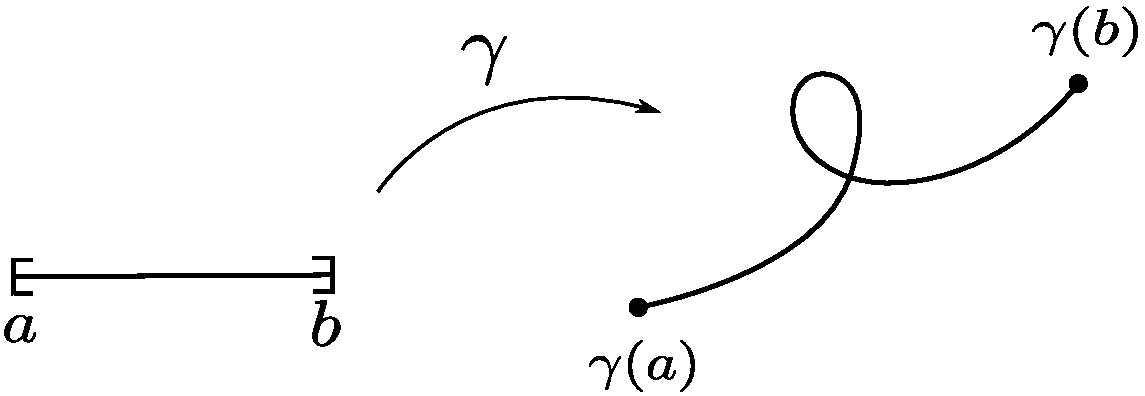
\includegraphics[scale = 0.5]{Figuras/Curva1.pdf}
    \caption{Definición de curva.}
    \label{fig:Curva1}
\end{figure}

\begin{defi}
\ 

\begin{enumerate}
\item Una curva $\gamma$ se dice de clase $C^1$ (o suave) a trazos si existe una partición finita $a = t_0 < t_1 < \cdots < t_n = b$ tal que $\gamma$ es derivable en $]t_{i-1},t_i[$ y $\gamma'(t)$ es continua en $[t_i, t_{i+1}]$; la continuidad en $[t_i, t_{i+1}]$ significa que los límites $\lim\limits_{t \to t_i^+} \gamma'(t)$ y $\lim\limits_{t\to t_{i+1}^-} \gamma'(t)$ existen.

\begin{figure}[H]
    \centering
    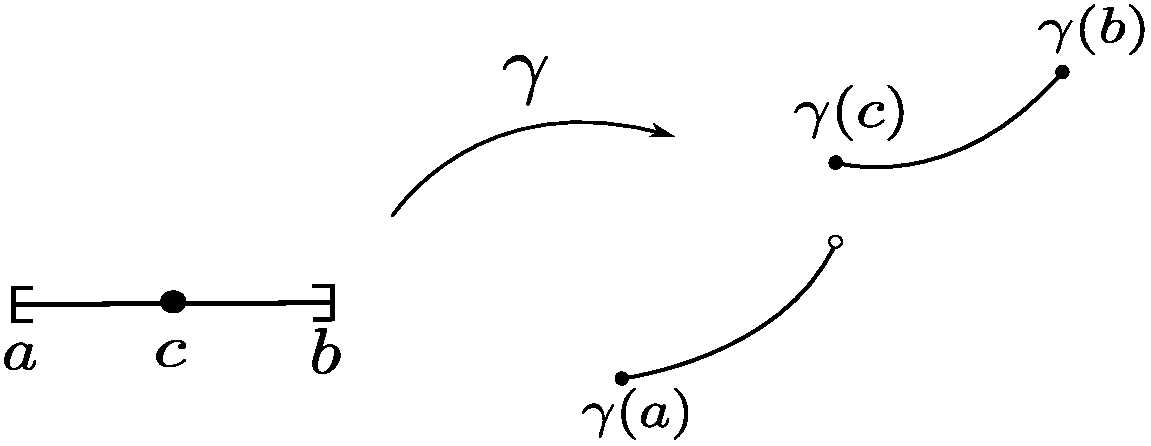
\includegraphics[scale = 0.5]{Figuras/Curva2.pdf}
    \caption{Curva suave a trazos.}
    \label{fig:Curva2}
\end{figure}

\item Una curva $\gamma : [a,b] \longrightarrow \mathbb{C}$ de clase $C^1$ se dice un \textbf{arco de Jordan} si $\gamma$ es inyectiva en $[a,b[$ (geométricamente, la curva no se cruza). Si además la curva es cerrada, la llamamos \textbf{curva de Jordan}.

\begin{figure}[H]
    \centering
    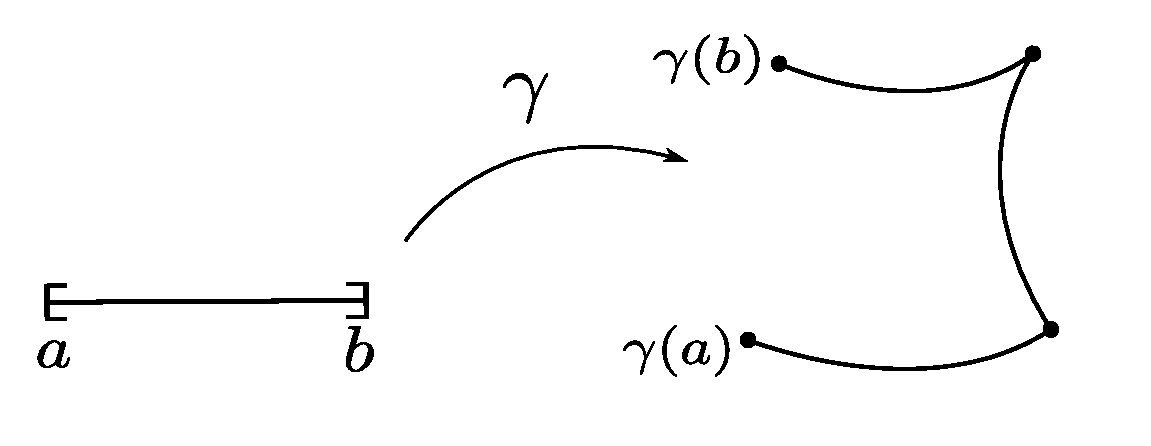
\includegraphics[scale = 0.5]{Figuras/Curva3.pdf}
    \caption{Arco de Jordan.}
    \label{fig:Curva3}
\end{figure}

\item Sea la curva $\gamma: [a,b] \longrightarrow \mathbb{C}$, se define la \textbf{curva opuesta} $- \gamma : [a,b] \longrightarrow \mathbb{C}$ como 
$$-\gamma(t) = \gamma(a+b-t).$$

\begin{figure}[H]
    \centering
    
\includegraphics[scale = 0.5]{Figuras/Curva4.pdf}
    \caption{Curva opuesta.}
    \label{fig:Curva4}
\end{figure}

\end{enumerate}

\begin{ejemplo}
Una parametrización de la circunferencia centrada en el complejo $z_0$ de radio $R$ es
$$\gamma(t) = z_0 + R e^{it}, \quad t \in [0,2\pi],$$

la cual es una curva de Jordan orientada en sentido antihorario.
\end{ejemplo}

\begin{ejemplo}
Una parametrización del segmento dirigido desde el complejo $z_1$ hasta el complejo $z_2$, denotado a veces por $[z_1,z_2]$, es 
$$\gamma(t) = z_1 + t(z_2 - z_1), \quad t\in [0,1],$$

la cual es un arco de Jordan.
\end{ejemplo}

\end{defi}

\begin{defi}
 Si $\gamma_1: [a,b] \longrightarrow \mathbb{C}$ y $\gamma_2: [b,c] \longrightarrow \mathbb{C}$ son dos curvas con $\gamma_1(b) = \gamma_2(b)$, entonces se define la \textbf{unión} o \textbf{suma} de ellas $\gamma_1 + \gamma_2: [a,c] \longrightarrow \mathbb{C}$ por 
\begin{equation*}
(\gamma_1 + \gamma_2)(t) = \left\{ \begin{array}{c}
\gamma_1(t), \quad t \in [a,b] \\
\gamma_2(t), \quad t \in [b,c]
\end{array}  \right. .
\end{equation*}
\end{defi}

\begin{figure}[H]
    \centering
    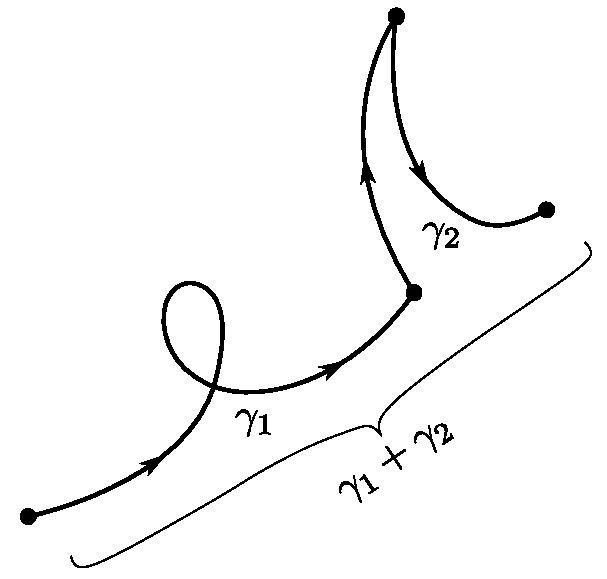
\includegraphics[scale = 0.5]{Figuras/Curva5.pdf}
    \caption{Unión de curvas.}
    \label{fig:Curva5}
\end{figure}

Claramente, si $\gamma_1$ y $\gamma_2$ son suaves por tramos, entonces también lo es $\gamma_1 + \gamma_2$.
\\

En general, sean $a, b, c,d \in \mathbb{R}$ con $a < b$ y $c < d$. Sean las curvas $\gamma_1 :[a,b] \longrightarrow \mathbb{C}$ y $\gamma_2 :[c,d] \longrightarrow \mathbb{C}$ tales que $\gamma_1(b) = \gamma_2(c)$. La suma de las curvas $\gamma_1 + \gamma_2: [a,b+(d-c)] \longrightarrow \mathbb{C}$ está definida por:
\begin{equation*}
(\gamma_1 + \gamma_2)(t) = \left\{ \begin{array}{cl}
\gamma_1(t), &\quad a \leq t \leq b \\
\gamma_2(t - (b-c)), &\quad b \leq t \leq b + (d-c)
\end{array}  \right. .
\end{equation*}

De manera natural se define la suma $\gamma_1 + \gamma_2 + \cdots + \gamma_n$ de un número finito de curvas tales que el extremo de $\gamma_j$ es el origen de $\gamma_{j-1}$ para $j = 2, \dots, n$.

\begin{defi}
Una curva (suave por tramos) $\tilde{\gamma} : [\tilde{a}, \tilde{b}] \longrightarrow \mathbb{C}$ se llama una \textbf{reparametrización} de $\gamma: [a,b] \longrightarrow \mathbb{C}$ si existe una función $\alpha: [a,b] \longrightarrow [\tilde{a}, \tilde{b}]$ de clase $C^1$ con $\alpha'(t) > 0$ para $t\in ]a,b[$, $\alpha(a) = \tilde{a}$ y $\alpha(b) = \tilde{b}$ tal que $\gamma(t) = \tilde{\gamma}(\alpha(t))$.
\end{defi}

\begin{figure}[H]
    \centering
    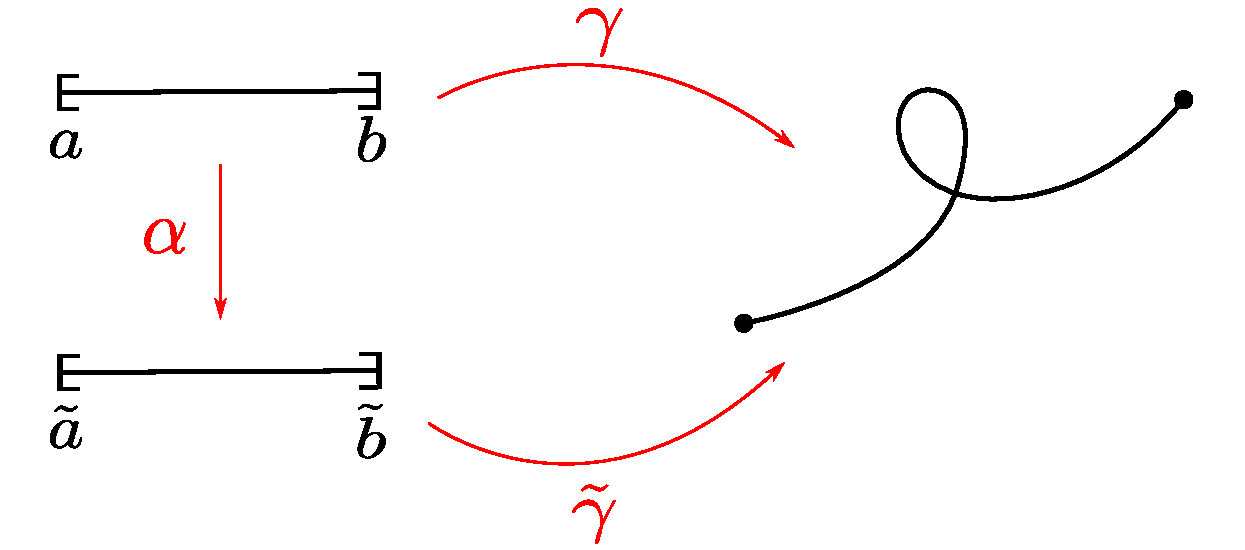
\includegraphics[scale = 0.5]{Figuras/Curva6.pdf}
    \caption{Reparametrización de una curva.}
    \label{fig:Curva6}
\end{figure}

\textbf{Observación}: Las condiciones $\alpha'(t) > 0$ (por lo que $\alpha$ es creciente), $\alpha(a) = \tilde{a}$ y $\alpha(b) = \tilde{b}$ implican que $\tilde{\gamma}$ recorre la curva en el mismo sentido que lo hace $\gamma$. La diferencia está en la velocidad en que se recorre la curva, ya que $\gamma'(t) = \tilde{\gamma}'(\alpha(t)) \cdot \alpha'(t)$. Si la función $\alpha$ fuera decreciente $(\alpha' <  0)$, la curva $\tilde{\gamma}$ sería una reparametrización de $\gamma$ recorrida en el sentido opuesto.

\section{Integral de línea}

\begin{defi}
Sea $f: A \subseteq \mathbb{C} \longrightarrow \mathbb{C}$ una función continua y sea $\gamma :[a,b] \longrightarrow \mathbb{C}$ una curva suave a trazos con $\gamma([a,b]) \subset A$ (la curva está contenida en $A$). Entonces,
$$\int_{\gamma} f  = \int_{\gamma} f(z)\, dz := \sum_{i=1}^n \int_{t_{i-1}}^{t_i} f(\gamma(t)) \gamma'(t) \,dt$$

se llama \textbf{integral de $f$ a lo largo de $\gamma$}.
\end{defi}

\textbf{Observación:} Si 
$$f(z) = u(x,y) + iv(x,y); ~ \gamma(t) = x(t) + iy(t); ~ \gamma'(t) = x'(t) + i y'(t),$$

entonces
\begin{align*}
f(\gamma(t)) \gamma'(t) &= [u(x(t), y(t)) + i v(x(t), y(t))] \cdot [x'(t) + i y'(t)] \\
&= u x' - v y' + i(uy'+vx').
\end{align*}

Así, 
\begin{equation*}
\int_{\gamma} f = \sum_{i=1}^n \int_{t_{i-1}}^{t_i} u x' - v y' + i(uy'+vx')\,dt  
= \sum_{i=1}^n \int_{t_{i-1}}^{t_i} (u x' - v y') \,dt + i \sum_{i=1}^n \int_{t_{i-1}}^{t_i} (uy'+vx') \,dt. 
\end{equation*}

Como $x'(t) dt = dx$ y $y'(t) dt = dy$, denotaremos esto último de la siguiente forma:
$$\int_{\gamma} f = \int_{\gamma} udx - vdy + i \int_{\gamma} vdx + udy.$$

\begin{teorema} \label{PropiedadesILinea}
Para funciones continuas $f,g$ y curvas suaves a trazos, $\gamma, \gamma_1, \gamma_2$, tenemos:

\begin{itemize}
\item $$\int_{\gamma} (c_1 f + c_2 g) = c_1 \int_{\gamma} f + c_2 \int_{\gamma} g, \quad c_1,c_2 \in \mathbb{C}.$$

\item $$\int_{-\gamma} f = - \int_{\gamma} f. $$

\item $$\int_{\gamma_1 + \gamma_2} f = \int_{\gamma_1} f + \int_{\gamma_2} f.$$
\end{itemize}
\end{teorema}

\begin{proof}
Ver apuntes de Cálculo III.
\end{proof}

\begin{teorema} \label{IntegralRepara}
Sea $f: A \subseteq \mathbb{C} \longrightarrow \mathbb{C}$ una función continua y sea $\gamma: [a,b] \longrightarrow \mathbb{C}$ una curva suave a tramos con $\gamma([a,b]) \subset A$ y $\tilde{\gamma}$ una reparametrización de $\gamma$. Entonces,
$$\int_{\gamma} f =  \int_{\tilde{\gamma}} f.$$

\end{teorema}

\begin{proof}
Sin pérdida de generalidad, podemos asumir que $\gamma$ es de clase $C^1$ en todo $[a,b]$.
$$\int_{\gamma} f = \int_a^b f(\gamma(t)) \gamma'(t)\,dt.$$

Ahora, como $\tilde{\gamma}$ es una reparametrización de $\gamma$ existe una función $\alpha: [a,b] \longrightarrow [\tilde{a}, \tilde{b}]$ de clase $C^1$ con $\alpha'(t) > 0$ para $t\in ]a,b[$, $\alpha(a) = \tilde{a}$ y $\alpha(b) = \tilde{b}$ tal que 
$$\gamma(t) = \tilde{\gamma}(\alpha(t)) ~\Rightarrow~ \gamma'(t) = \tilde{\gamma}'(\alpha(t)) \alpha'(t).$$

Luego, 
\begin{align*}
\int_{\gamma} f &= \int_a^b f(\tilde{\gamma}(\alpha(t))) \tilde{\gamma}'(\alpha(t)) \alpha'(t) \,dt \\
&= \int_{\tilde{a}}^{\tilde{b}} f(\tilde{\gamma}(s)) \tilde{\gamma}'(s)\,ds \qquad (s = \alpha(t) \Rightarrow ds = \alpha'(t) dt) \\
&= \int_{\tilde{\gamma}} f.
\end{align*}
\end{proof}

\begin{ejemplo}
Calcular
$$\int_C \overline{z} \,dz$$

donde $C$ es la mitad derecha de la circunferencia $|z| = 2$ orientada en sentido antihorario.
\\

\textbf{Solución:} Una parametrización de $C$ es
$$\gamma: [- \pi/2, \pi/2] \longrightarrow \mathbb{C}, \gamma(t) = 2 e^{i t}.$$

\begin{figure}[H]
    \centering
    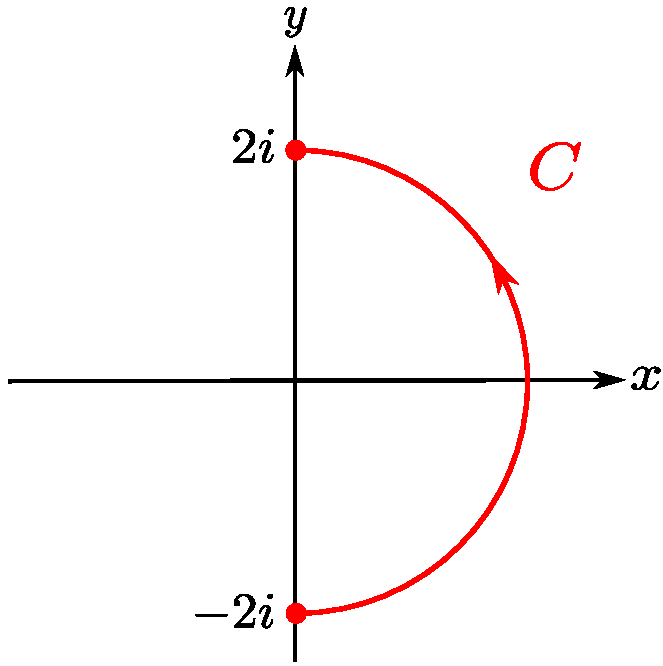
\includegraphics[scale = 0.5]{Figuras/Integral1.pdf}
    \caption{Mitad derecha de la circunferencia $|z| = 2$.}
    \label{fig:IntegralLinea1}
\end{figure}

\vspace{-0.4cm}

Tenemos que $C$ es suave con 
$$\gamma'(t) = 2 i e^{i t}.$$

Luego, por definición, 
\begin{equation*}
\int_C \overline{z} \,dz = \int_{- \pi/2}^{\pi/2} 2 e^{-it} 2 i e^{i t} \,dt = 4i \int_{-\pi/2}^{\pi/2}\, dt = 4 \pi i.
\end{equation*}
\end{ejemplo}

\begin{ejemplo}
Calcular
$$\int_C f(z) \,dz$$

donde $f(z) = y - x - i3x^2$ y $C$ es la unión del segmento que va desde 0 a $i$ y del segmento desde $i$ a $1+i$.
\\

\textbf{Solución}:  Sea $C_1$ el segmento desde $0$ a $i$ y $C_2$ el segmento desde $i$ a $1+i$, tenemos que
$$\int_C f(z) \,dz = \int_{C_1} f(z) \,dz + \int_{C_2} f(z) \,dz.$$

\begin{figure}[H]
    \centering
    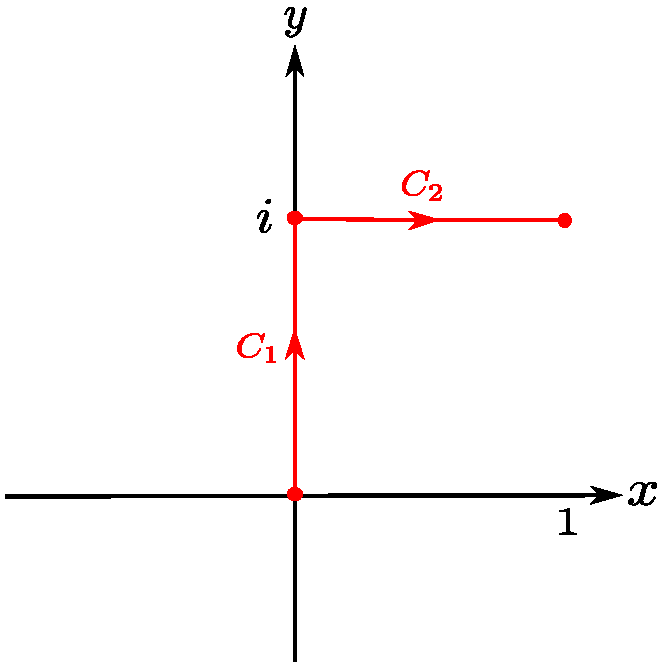
\includegraphics[scale = 0.5]{Figuras/Integral2.pdf}
    \caption{Unión del segmento desde $0$ a $i$ y del segmento $i$ a $1+i$.}
    \label{fig:IntegralLinea2}
\end{figure}

Las parametrizaciones para $C_1$ y $C_2$ son, respectivamente,
\begin{align*}
\gamma_1: [0,1] \longrightarrow \mathbb{C}, \gamma_1(t) &= it \\
\gamma_2: [0,1] \longrightarrow \mathbb{C}, \gamma_2(t) &= t + i
\end{align*}

Entonces, $C = C_1 + C_2$ es suave por trazos con 
$$\gamma_1\,'(t) = i ~~\mbox{y}~~ \gamma_2\,'(t) = 1.$$

Por definición,
\begin{align*}
\int_{C_1} f &= \int_0^1 t i \,dt = \left. i \frac{t^2}{2} \right|_0^1 = \frac{i}{2}, \\
\int_{C_2} f &= \int_0^1 (1-t-i3t^2) 1 \,dt = \left. t - \frac{t^2}{2} - it^3 \right|_0^1 = \frac{1}{2} - i.
\end{align*}

Por lo tanto, 
$$\int_C f(z) \,dz = \frac{i}{2} + \frac{1}{2} - i = \frac{1}{2} - \frac{i}{2}.$$
\end{ejemplo}

De Cálculo III, sabemos que si $\gamma$ es un arco de Jordan, ésta es rectificable y su longitud viene dada por 
$$l(\gamma) = \int_a^b |\gamma'(t)| \,dt = \int_a^b \sqrt{[x'(t)]^2 + [y'(t)]^2} \,dt$$

y que es independiente de la parametrización de $\gamma$.

\begin{teorema} \label{CotaIntegral}
Sea $f: A \subseteq \mathbb{C} \longrightarrow \mathbb{C}$ una función  continua y sea $\gamma: [a,b] \longrightarrow \mathbb{C}$ una curva suave por tramos con $\gamma([a,b]) \subset A$. Si existe una constante $M > 0$ tal que $|f(z)| \leq M$ para todo los puntos $z$ traza de $\gamma$\footnote{ Que $z$ sea parte de la traza de $\gamma$ significa que existe $t \in [a,b]$ tal que $z = \gamma(t)$.  }, entonces
$$\left|\int_{\gamma} f \right| \leq M l(\gamma).$$

Más general, tenemos
$$\left|\int_{\gamma} f \right| \leq \int_{\gamma} |f| \,|dz|$$

donde la última integral se define como 
$$\int_{\gamma} |f| |dz| := \int_a^b |f(\gamma(t))|\, |\gamma'(t)| \,dt.$$
\end{teorema}

\begin{proof}

Supongamos, sin pérdida de generalidad, que la curva $\gamma$ es suave. Entonces, podemos escribir
\begin{align*}
\left| \int_{\gamma} f \right| &= \left| \int_a^b f(\gamma(t)) \gamma'(t) \,dt \right| \\
&\leq \int_a^b |f(\gamma(t)) \gamma'(t)| \,dt = \int_a^b |f(\gamma(t))| \, |\gamma'(t)| \,dt.
\end{align*}

Como $|f(\gamma(t))| \leq M$ para todo $t \in [a,b]$, la expresión nos queda
\begin{equation*}
\int_a^b |f(\gamma(t))| \, |\gamma'(t)| \,dt \leq M \int_a^b |\gamma'(t)| \,dt = M l(\gamma).
\end{equation*}

\end{proof}

\begin{ejemplo}
Sea $\gamma$ la mitad de la circunferencia unitaria descrita contraria a las agujas del reloj. Mostrar que 
$$\left| \int_{\gamma} \frac{e^z}{z}\right| \leq \pi e.$$

\textbf{Solución}: Notemos que 
$$l(\gamma) = \int_0^{\pi} |\gamma'(t)| \,dt = \pi$$

pues $\gamma(t) = e^{it}, 0 \leq t \leq \pi$ y $\gamma'(t)= i e^{it}$. 

Ahora, para $z$ en la semi-circunferencia, descrita por $\gamma$, existe $t \in [0,\pi]$ tal que $z = e^{it} = \cos t + i \sin t$ y 
$$\left| \frac{e^z}{z}\right| = \frac{|e^{\cos t} e^{i\sin t}|}{|e^{it}|} = \frac{e^{\cos t}}{1} \leq e = M.$$

Así,
$$\left| \int_{\gamma} \frac{e^z}{z}\right| \leq \pi e.$$
\end{ejemplo}

\section{Independencia del camino}

El siguiente teorema es análogo al Teorema Fundamental del Cálculo:

\begin{teorema} \label{TFClinea}
Sea $f: A \subseteq \mathbb{C} \longrightarrow \mathbb{C}$ una función continua tal que $f = F\,'$ para alguna función analítica $F: A \longrightarrow \mathbb{C}$. Sea $\gamma: [a,b] \longrightarrow \mathbb{C}$ una curva suave a trazos con $\gamma([a,b]) \subseteq A$ y que une los puntos $\gamma(a) = z_1$ y $\gamma(b) = z_2$. Entonces,
$$\int_{\gamma} f = F(z_2) - F(z_1).$$

En particular, si $z_1 = z_2$ (es decir, una curva cerrada), entonces
$$\int_{\gamma} f = 0.$$
\end{teorema}

\begin{proof}
Por regla de la cadena, tenemos que 
$$(F \circ \gamma)'(t) = F\,'(\gamma(t)) \gamma\,'(t) = f(\gamma(t)) \gamma\,'(t).$$

Así,
\begin{align*}
    \int_{\gamma} f = \int_a^b f(\gamma(t)) \gamma\,'(t) \,dt &= \int_a^b (F \circ \gamma)'(t) \,dt \\
    &= F(\gamma(b)) - F(\gamma(a))\\
    &= F(z_2) - F(z_1).
\end{align*} 
\end{proof}

\begin{defi}
Toda función $F$ tal que $f = F\,'$ para todo $z$ en un dominio $D$, se llama \textbf{primitiva} o \textbf{antiderivada} de $f$
\end{defi}

\begin{teorema}[Independencia del camino]  \label{TFC2}
Sea $f(z)$ una función continua en un abierto conexo $D$ (una región). Si cualquiera de estas afirmaciones es verdadera, lo son también las demás:
\begin{itemize}
    \item[a)] $f$ tiene una primitiva $F$ en $D$;
    
    \item[b)] las integrales de $f$ a lo largo de curvas contenidas en $D$ que unen puntos fijos $z_1$ y $z_2$ tienen todas el mismo valor;
    
    \item[c)] las integrales de $f$ a lo largo de cualquier curva cerrada contenida en $D$ es cero.
\end{itemize}
\end{teorema}

\begin{proof}
Para demostrar el teorema es suficiente probar las equivalencias entre a) y b); b) y c).

\begin{itemize}
    \item $a) \Rightarrow b)$: Directo del teorema \ref{TFClinea}.
    
    \item $b) \Rightarrow a)$: Necesitamos mostrar que si la integral es independiente de la curva, entonces $f$ tiene una antiderivada $F$. Fijamos $z_0 \in D$ y definimos
    $$F(z) = \int_{\gamma(z_0,z)} f(\xi) \,d\xi,$$
    
    donde $\gamma(z_0,z)$ es una curva que une $z_0$ y $z$, ver figura \ref{fig:IntegralLinea1}. Tal curva existe porque $D$ es conexo. Esto define una función $F$ en $D$ sin ambigüedad alguna, pues b) nos dice que el valor de $F(z)$ depende de $z$ y no de la trayectoria elegida, en tanto se encuentre en $D$. 
    
    Sea $\varepsilon > 0$, como $D$ es abierto y $f$ es continua en $z$, existe un número $\delta > 0$ tal que la bola abierta $B(z, \delta) \subseteq D$ y $|f(\xi) - f(z)| < \varepsilon$ siempre que $|\xi - z| < \delta$. Si escogemos $z+w \in B(z, \delta)$ y conectamos $z$ a $z+w$ por medio de un segmento $[z,z+w]$. Entonces, todo $[z,z+w]$ descansa en $B(z,\delta)$, ver figura \ref{fig:IntegralLinea1},  y
    $$F(z+w) - F(z) = \int_{\gamma(z_0,z) + [z,z+w]} f(\xi) \,d\xi - \int_{\gamma(z_0,z)} f(\xi) \,d\xi = \int_{[z,z+w]} f(\xi) \,d\xi.$$
    
    Así, si $|(z+w)-z| = |w| < \delta$, se cumple que
    \begin{align*}
       \left|\frac{F(z+w)-F(z)}{w} - f(z)\right| &=  \frac{|F(z+w) - F(z) - w f(z)|}{|w|} \\
       &= \frac{1}{|w|} \left| \int_{[z,z+w]} f(\xi) \,d\xi -f(z) \int_{[z,z+w]} 1 \,d\xi  \right| \\
       &= \frac{1}{|w|} \left| \int_{[z,z+w]} [f(\xi) - f(z)] \,d\xi   \right| \\
       &\leq \frac{\varepsilon}{|w|}l([z,z+w]) \quad (Teorema \ref{CotaIntegral})\\
       &= \frac{\varepsilon}{|w|} |w| = \varepsilon.
    \end{align*}

Probando así que
$$\lim_{w \to 0} \frac{F(z+w)- F(z)}{w} = f(z),$$

ésto es, $F$ es derivable y $F\,' = f$.

   \begin{figure}[H]
        \centering
        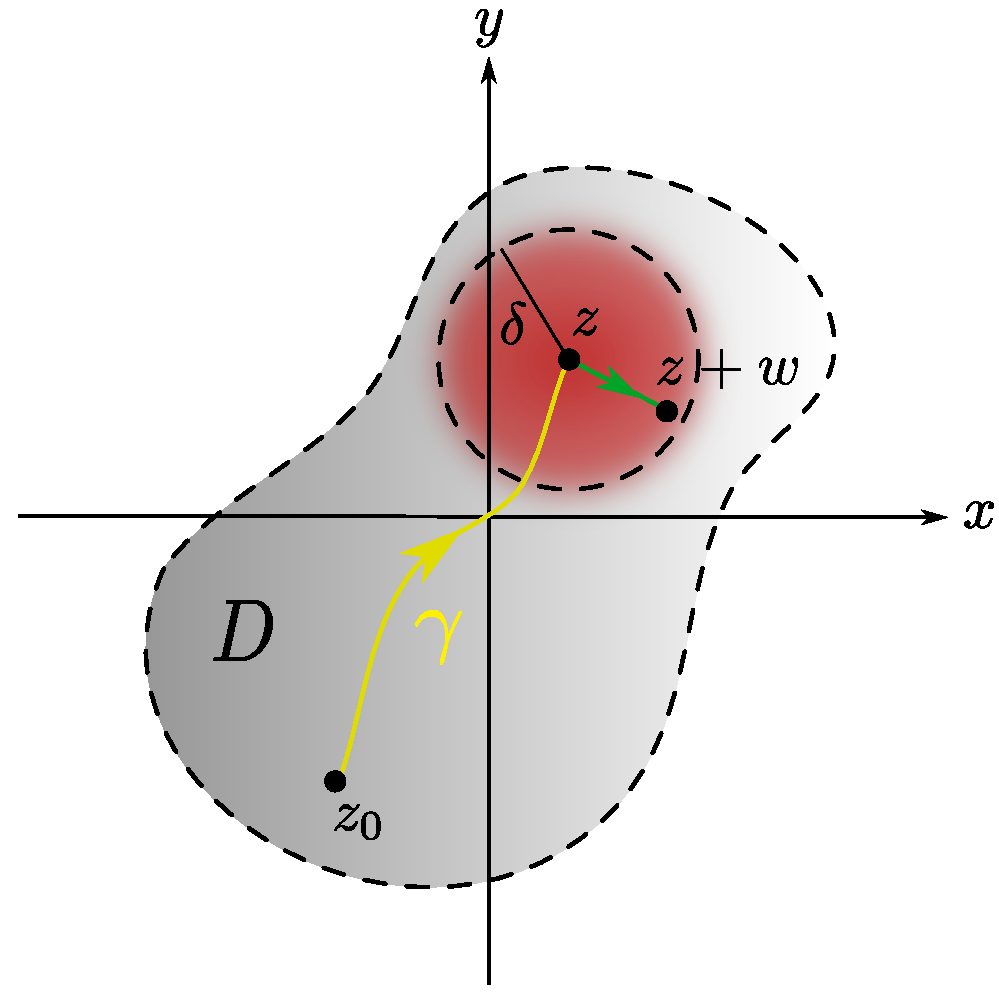
\includegraphics[scale = 0.45]{Figuras/TFCIntegralLinea1.pdf}
        \caption{Visión geométrica de la demostración.}
        \label{fig:TFC1}
    \end{figure}

\item $b) \Rightarrow c)$: Es directo de usar a).

\item $c) \Rightarrow a)$: Consideremos dos curvas $\gamma_1$ y $\gamma_2$ suaves por trazos que unen dos puntos $z_1$ y $z_2$ en $D$, y sea $\Gamma$ la curva cerrada que surge al unir $\gamma_1$ y $- \gamma_2$. Entonces,
$$0 = \int_{\Gamma} f(z) \,dz = \int_{\gamma_1} f(z) \,dz + \int_{-\gamma_2} f(z) = \int_{\gamma_1} f(z) \,dz - \int_{\gamma_2} f(z),$$
implicando que 
$$\int_{\gamma_1} f(z) \,dz = \int_{\gamma_2} f(z) \,dz.$$

Por lo tanto, la integral de $f$ es independiente de la curva.

 \begin{figure}[H]
        \centering
        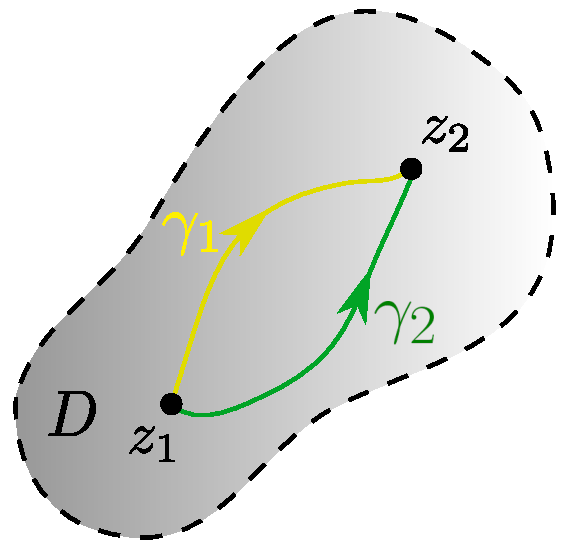
\includegraphics[scale = 0.45]{Figuras/TFCIntegralLinea2.pdf}
        \caption{Dos curvas con los mismos extremos.}
        \label{fig:TFC2}
    \end{figure}
\end{itemize}
\end{proof}

\begin{ejemplo}
Calcular
$$\int_{\gamma} e^z dz,$$

donde $\gamma(t) = e^{it}$, $0 \leq t \leq \pi.$
\\

\textbf{Solución:} La función $e^z$ es continua en todo el plano complejo, con antiderivada $e^z$. El punto inicial de $\gamma$ es $z_1 = \gamma(0) = 1$ y su punto terminal es $z_2 = \gamma(\pi) = -1$. Entonces,
$$\int_{\gamma} e^z dz = \left. e^z \right|_{1}^{-1} = e^{-1}-e^1 = - 2 \sinh(1).$$
\end{ejemplo}

\begin{ejemplo}
Evaluar 
$$\int_C \frac{1}{z} dz,$$

donde $C$ es el camino poligonal que parte de $1$ al $2+i$ y termina en $3$, ver figura \ref{fig:EjTFC1}.
\\

\textbf{Solución:} La función $1/z$ es continua en $\mathbb{C} \setminus \{0\}$. Una antiderivada de $1/z$ es $Log(z) = \ln |z| + i Arg(z)$ en la región $D = \mathbb{C}\setminus ]-\infty, 0]$. La curva $C$ yace enteramente en $D$, ver figura \ref{fig:EjTFC1}.

   \begin{figure}[H]
        \centering
        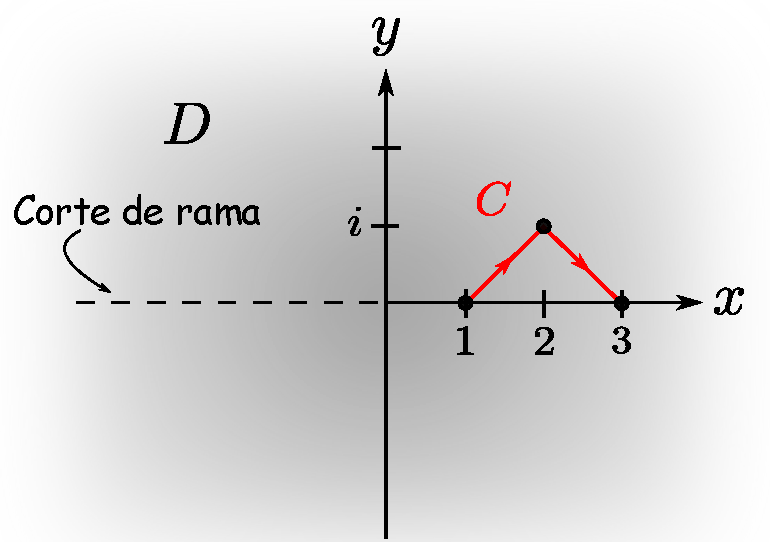
\includegraphics[scale = 0.5]{Figuras/Ejemplo_TFCIntegralLinea1.pdf}
        \caption{Camino poligonal que inicia del $1$ se va al $2+i$ y termina en $3$.}
        \label{fig:EjTFC1}
    \end{figure}
    
Así, 
$$\int_C \frac{1}{z} dz = \left. Log(z) \right|_1^3 = \ln(3).$$
\end{ejemplo}

\begin{ejemplo}
Evaluar 
$$\int_C \frac{1}{z} dz,$$

donde $C$ es el camino poligonal que parte de $-1$ al $-1+i$ y termina en $-2-2i$, ver figura \ref{fig:EjTFC2}.
\\

\textbf{Solución:} Para aplicar el teorema debemos encontrar una antiderivada de $1/z$ que sea analítica en la región que contiene a la curva $C$. En este caso, no podemos usar $Log(z)$ como antiderivada porque no es analítica en una región que contenga a $C$ (la curva pasa por el corte de ramificación). En su lugar, debemos usar otra rama del logaritmo. Sabemos que al considerar $\alpha < \arg(z) < \alpha + 2\pi$ para un cierto $\alpha \in \mathbb{R}$, se obtiene una rama de $\log(z)$ analítica. 

Tomando, por ejemplo, $\alpha = 0$, podemos escribir 
$$\log(z) \rightarrow \log_0(z) = \ln|z| + i \arg_0(z),$$

donde $0 < \arg_0(z) < 2\pi$, la cual es una antiderivada de $1/z$, analítica en la región $D = \mathbb{C}\setminus [0, +\infty[$ donde yace la curva $C$. Así,
\begin{align*}
    \int_C \frac{1}{z} dz &= \log_0(-2-2i) - \log_0(-1) \\
    &= \ln|-2-2i| + i \arg_0(-2-2i) - (\ln(1) + i \arg_0(-1)) \\
    &= \frac{1}{2} \ln(8) + i \frac{5\pi}{4} - i \pi = \frac{3}{2} \ln(2) + i\frac{\pi}{4}.
\end{align*}

\begin{figure}[H]
        \centering
        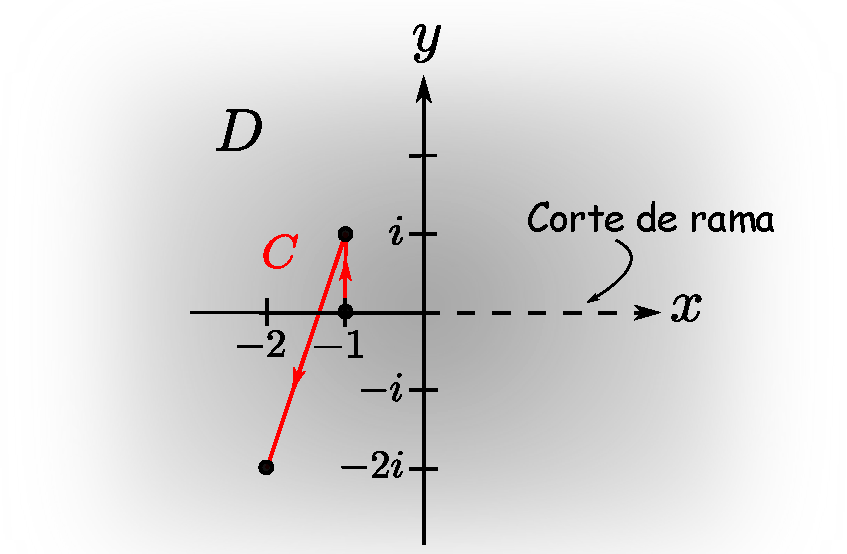
\includegraphics[scale = 0.5]{Figuras/Ejemplo_TFCIntegralLinea2.pdf}
        \caption{Camino poligonal que inicia del $-1$ se va al $-1+i$ y termina en $-2-2i$.}
        \label{fig:EjTFC2}
    \end{figure}
\end{ejemplo}

\section{Teorema de Cauchy-Goursat}

Recordemos el teorema de Green en su primera forma del Cálculo III.

\begin{teorema}[de Green primera forma]
Sea $\gamma$ una curva de Jordan con orientación positiva y sea $R$ la reunión de $C$ y de su interior. Si $\Vec{F}(x,y) = P(x,y) \hat{\imath} + Q(x,y) \hat{\jmath}$ es de clase $C^1$ en un abierto $A$ que contiene a $R$, entonces
$$\oint_{\gamma} Pdx + Qdy = \iint_R \left[ \frac{\partial Q}{\partial x} - \frac{\partial P}{\partial y}\right] \,d(x,y).$$
\end{teorema}

Este teorema permite demostrar el siguiente resultado.

\begin{teorema}[de Cauchy]
Si $f$ es analítica en todos los puntos encerrados por una curva simple cerrada $\gamma$ y $f'$ es continua en dicha región, entonces
$$\int_{\gamma} f = 0.$$
\end{teorema}

\begin{proof}
Consideremos $f(z) = u(x,y) + iv(x,y)$ una función analítica en una región $R$ que contiene el interior de la curva $\gamma$, que supondremos de orientación positiva, y su frontera. Entonces, como $f'(z) = u_x + i v_x = v_y - iu_y$  es continua, $u$ y $v$ tienen derivadas parciales continuas. De esta manera, podemos aplicar el teorema de Green en su primera forma y obtener que
\begin{align*}
    \int_{\gamma} udx - vdy &= - \iint_R (v_x + u_y) \,d(x,y), \\
    \int_{\gamma} vdx + udy &=  \iint_R (u_x - v_y) \,d(x,y).
\end{align*}

Por las ecuaciones de Cauchy-Riemann, concluimos que ambas integrales son nulas. Así,
$$\int_{\gamma} f = \int_{\gamma} udx - vdy + i \int_{\gamma} vdx + udy = 0.$$

Si la curva tiene orientación negativa, la conclusión es la misma.

\end{proof}

Goursat fue el primero en demostrar que la condición de continuidad de $f'$ se puede omitir, dando paso a la versión modificada del teorema de Cauchy, conocida como el \textbf{teorema de Cauchy-Goursat} cuya demostración se escapa del curso.

\begin{teorema}[de Cauchy-Goursat]
Si $f$ es analítica en todos los puntos encerrados por una curva simple cerrada $\gamma$, entonces
$$\int_{\gamma} f = 0.$$
\end{teorema}

\textbf{Observación:} Consideremos la función $f(z) = \frac{1}{z}$ y supongamos que $\gamma$ es la circunferencia centrada en el origen de radio 1. $f$ es analítica en todo punto excepto en $z = 0$.

Por otro lado,
\begin{equation}
 \int_{\gamma} \frac{1}{z} = \int_0^{2\pi} \frac{1}{e^{it}} i e^{it} dt = \int_0^{2\pi} i  dt = 2\pi i \neq 0. \label{PreTIC}  
\end{equation}

Esto nos dice que, la hipótesis de analiticidad en todo el interior no puede ser debilitada.

\section{Dominios simplemente conexos y múltiplemente conexos}

\begin{defi}
Sea $D$ un abierto conexo del plano complejo. Se dice que $D$ es una \textbf{región simplemente conexa} si toda curva simple cerrada en $D$ encierra sólo puntos de $D$, en otras palabras, $D$ no tiene agujeros. Los conjuntos que no son simplemente conexos se llaman \textbf{múltiplemente conexos}.
\end{defi}

\begin{figure}[H]
    \centering
    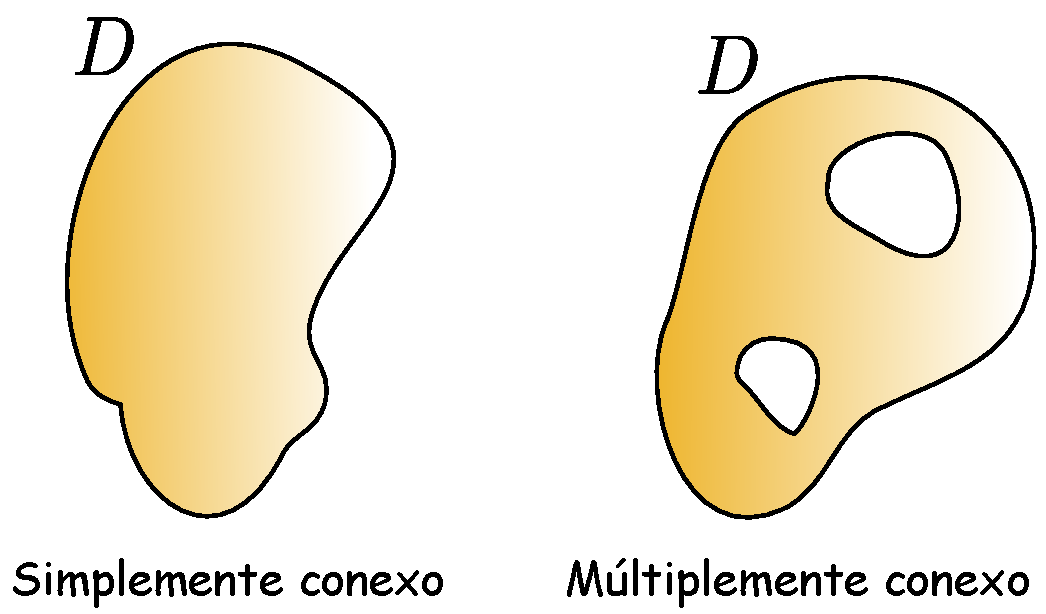
\includegraphics[scale = 0.5]{Figuras/SimplementeConexo.pdf}
    \caption{Dominios simplemente conexo y múltiplemente conexo.}
    \label{fig:SimConexo}
\end{figure}

El teorema de Cauchy-Goursat admite la siguiente extensión relativa a dominios simplemente conexos.

\begin{teorema} \label{CG-SC}
Si una función $f$ es analítica en un dominio simplemente conexo $D$, entonces 
$$\int_{\gamma} f(z) \,dz = 0$$

para toda curva cerrada $\gamma$ contenida en $D$.
\end{teorema}

\begin{proof}
Consulte la sección 3.6 de \cite{Asmar}.
\end{proof}

\begin{corolario}
Una función $f$ que es analítica sobre un dominio simplemente conexo $D$ tiene primitiva en $D$ y la integral es independiente de la curva que une a dos puntos $z_1,z_2 \in D$.
\end{corolario}

\begin{proof}
Consecuencia inmediata del teorema \ref{CG-SC}, a causa del teorema \ref{TFC2}.
\end{proof}

El teorema de Cauchy-Goursat se puede extender a dominos múltiplemente conexos

\begin{teorema} \label{CGMultiConexo}
Sea $\gamma$ una curva simple cerrada y sean $\gamma_1, \gamma_2, \dots, \gamma_n$ curvas simples cerradas que se encuentran al interior de $\gamma$ y éstas no se cortan. Sea $R$ la región de todo los puntos al interior de $\gamma$ y al exterior de $\gamma_j$, $j = 1,2, \dots, n$. Entonces, $f$ analítica en $R$ implica que 
$$\int_{\gamma} f = \sum_{j=1}^n \int_{\gamma_j} f,$$

donde se asume que las orientaciones de las curvas son positivas.
\end{teorema}

\begin{proof}
Fijemos un punto $z_0$ en la curva $\gamma$. Por medio de un segmento $L_1$ unimos $z_0$ a un punto $w_1$ en $\gamma_1$. Escogemos $z_1$ en $\gamma_1$ y consideramos la curva $\alpha_1$ que parte de $w_1$ hacia $z_1$ siguiendo la curva $\gamma_1$, pero en sentido contrario. 

Ahora, por medio de un segmento $L_2$ unimos $z_1$ con un punto $w_2$ en $\gamma_2$. Escogemos $z_2$ en $\gamma_2$ y consideramos la curva $\alpha_2$ que parte de $w_2$ hacia $z_2$ siguiendo la curva $\gamma_2$, en sentido contrario, ver figura \ref{fig:GeneralTCG}.

\begin{figure}[H]
    \centering
    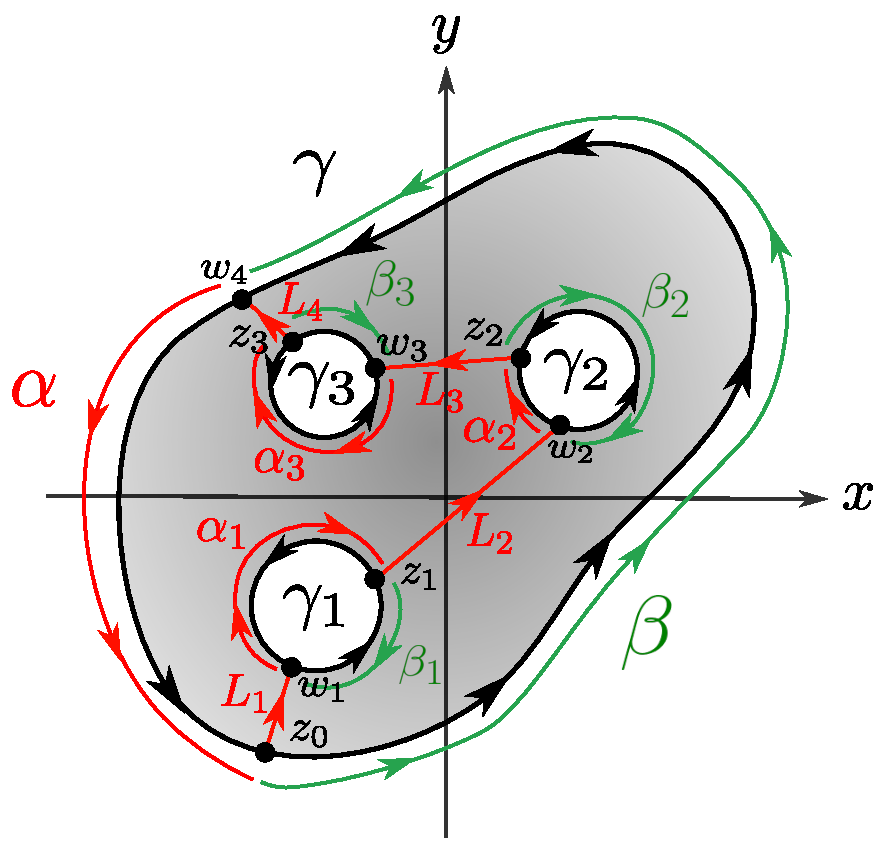
\includegraphics[scale = 0.52]{Figuras/GeneralTCG.pdf}
    \caption{Visión gráfica de la demostración.}
    \label{fig:GeneralTCG}
\end{figure}

Continuamos el proceso hasta encontrar puntos $w_n$ y $z_n$ en $\gamma_n$ y consideramos la curva $\alpha_n$ que parte de $w_n$ hacia $z_n$ siguiendo la curva $\gamma_n$, en sentido contrario. Al final, unimos $z_n$ a un punto $w_{n+1}$ en $\gamma$ mediante un segmento $L_{n+1}$ que no intersecte el camino previo seleccionado de $z_0$ a $z_n$, pasando a través de $w_1, z_1, w_2, z_2, \dots, w_n$. En la selección de estos puntos hemos definido:

\begin{quote}
    La curva $\alpha_j$ que parte del punto $w_j$ hacia $z_j$ siguiendo la curva $\gamma_j$, en sentido contrario, para $j = 1, \dots, n$.
\end{quote}

Ahora definimos:
    
\begin{quote}
  La curva $\beta_j$ como aquella que parte del punto $z_j$ hacia $w_j$ siguiendo la curva $\gamma_j$, en sentido contrario.   
\end{quote}

Ahora, sea $\alpha$ parte de la curva $\gamma$ de $w_{n+1}$ a $z_0$ y sea $\beta$ parte de la curva $\gamma$ de  $z_0$ a $w_{n+1}$, ambas siguiendo el mismo sentido que $\gamma$.

La construcción hecha lleva a dos curvas cerradas $\Gamma_1$ y $\Gamma_2$, ver figura \ref{fig:GeneralTCG}, definidas como sigue:
\begin{align*}
\Gamma_1 &= \alpha + L_1 + \alpha_1 + \cdots + L_{n} + \alpha_n + L_{n+1}, \\
\Gamma_2 &= -L_{n+1} + \beta_n - L_{n} + \cdots + \beta_1 - L_1 + \beta.
\end{align*}

Como $f$ es analítica en $R$, será analítica en los dominios simplemente conexos formados por los interiores de $\Gamma_1$ y $\Gamma_2$. Entonces, por el teorema \ref{CG-SC},
$$\int_{\Gamma_1} f(z) \,dz = 0 ~~\mbox{y}~~ \int_{\Gamma_2} f(z) \,dz = 0.$$

Sumando ambas igualdades, obtenemos que
$$\int_{\Gamma_1} f(z) \,dz  + \int_{\Gamma_2} f(z) \,dz = 0.$$

Dado que
$$\int_{-L_j} f(z) \,dz = - \int_{L_j} f(z)\,dz, \quad j = 1,2, \dots, n+1,$$

concluimos que
$$\int_{\alpha} f(z) \,dz + \int_{\beta} f(z) \,dz + \sum_{j=1}^n \left(\int_{\alpha_j} f(z) \,dz + \int_{\beta_j} f(z) \,dz\right) = 0.$$

Pero,
$$\int_{\alpha_j} f + \int_{\beta_j} f = - \int_{\gamma_j} f ~~\mbox{y}~~ \int_{\alpha} f + \int_{\beta} f = \int_{\gamma} f.$$

Por lo tanto,
$$\int_{\gamma}f(z) \,dz - \sum_{j=1}^n \int_{\gamma_j} f(z) \,dz = 0 \Rightarrow \int_{\gamma} f(z) \,dz= \sum_{j=1}^n \int_{\gamma_j} f(z) \,dz. $$

\end{proof}



\begin{ejemplo}
Sea 
$$f(z) = \frac{1}{z^2(z^2 + 9)}$$

y consideremos el dominio simplemente conexo encerrado por las curvas $\gamma(t) = 2e^{it}$ y $\gamma_1(t) = e^{it}$, $0 \leq t \leq 2\pi$. $f$ es analítica en el interior de $\gamma$ y el exterior de $\gamma_1$. Entonces,
$$\int_{\gamma} \frac{1}{z^2(z^2+9)} = \int_{\gamma_1}\frac{1}{z^2(z^2+9)}.$$
\end{ejemplo}

El ejemplo se puede generalizar al siguiente corolario, el cual es una consecuencia particular del teorema \ref{CGMultiConexo}.

\begin{corolario} \label{CorolarioTCG}
Sean $\gamma_1$ y $\gamma_2$ dos curvas simples cerradas orientadas positivamente, donde $\gamma_2$ es interior a $\gamma_1$ (ver figura \ref{fig:CorlarioTCG}). Si una función $f$ es analítica en la región cerrada que forman esas curvas y los puntos situadas entre ellos, entonces
$$\int_{\gamma_1} f(z) \,dz = \int_{\gamma_2} f(z) \,dz.$$
\end{corolario}

\begin{figure}[H]
    \centering
    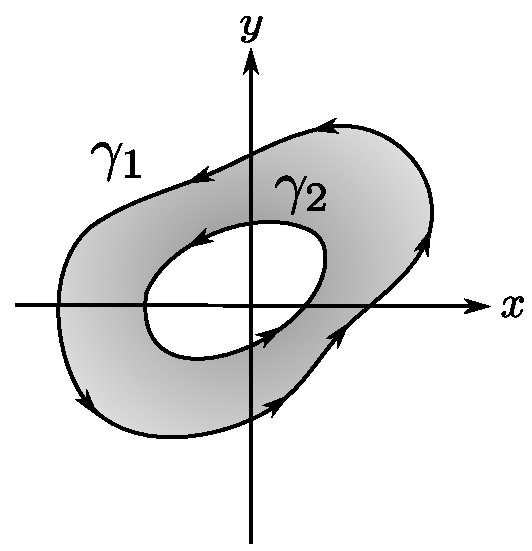
\includegraphics[scale = 0.6]{Figuras/CorolarioTCG.pdf}
    \caption{Principio de deformación de caminos.}
    \label{fig:CorlarioTCG}
\end{figure}

\textbf{Observación:} El corolario se conoce como el \textbf{principio de deformación de caminos}, ya que nos dice que si $\gamma_1$ se deforma continuamente en $\gamma_2$ pasando siempre por puntos en los que $f$ es analítica, el valor de la integral de $f$ sobre $\gamma_1$ no cambia.

\section{Fórmula de Integración de Cauchy}

Según lo calculado en \eqref{PreTIC},
si $\gamma$ es la circunferencia unitaria $\gamma(t) = e^{it}, 0 \leq t \leq 2\pi$, tenemos que
$$\int_{\gamma} \frac{1}{z} \,dz = 2\pi i$$

o, equivalentemente,
$$1 = \frac{1}{2\pi i} \int_{\gamma} \frac{1}{z} \,dz. $$

Notemos que $\gamma$ es cerrada e inyectiva en el intervalo $[0,2\pi[$. 

Ahora, consideremos una nueva curva $\alpha(t) = e^{it}, 0\leq t \leq 4\pi$ y repitamos el cálculo anterior
$$\int_{\alpha} \frac{1}{z} \,dz = \int_0^{4\pi} \frac{1}{e^{it}} i e^{it} \,dt = \int_0^{4\pi} i dt = 4\pi i,$$

es decir,
$$2 = \frac{1}{2\pi i} \int_{\alpha} \frac{1}{z} \,dz.$$

De forma inductiva, si $n \in \mathbb{N}$, entonces
$$n = \frac{1}{2\pi i} \int_{\gamma_n} \frac{1}{z} \,dz,$$

donde $\gamma_n(t) = e^{it}, 0 \leq t \leq 2n\pi.$

Finalmente, si $\tilde{\gamma}$ es otra curva cerrada, que envuelve al origen y que puede deformarse en alguna $\gamma_n$, ésto es, se puede aplicar el corolario \ref{CorolarioTCG}. Entonces,
$$n = \frac{1}{2\pi i} \int_{\gamma_n} \frac{1}{z} \,dz =  \frac{1}{2\pi i} \int_{\tilde{\gamma}} \frac{1}{z} \,dz.$$

Notemos que este número $n$ indica las veces que gira la curva en torno del origen y éste será positivo si gira contrario a las agujas del reloj y será negativo en el otro caso (segundo postulado del teorema \eqref{PropiedadesILinea}).

En general, para cualquier punto $z_0 \in \mathbb{C}$, se ve que el número de veces que una curva cerrada $\tilde{\gamma}$ gira alrededor de $z_0$ es
$$n = \frac{1}{2\pi i} \int_{\tilde{\gamma}}\frac{1}{z-z_0} \,dz$$

por un argumento similar. Observemos que si $z_0$ está al exterior de $\gamma$, entonces
$$0 = \frac{1}{2\pi i} \int_{\gamma} \frac{1}{z-z_0} \,dz.$$

Esta idea conduce a formular la siguiente definición.

\begin{defi}
Sea $\gamma$ una curva cerrada que envuelve al punto $z_0 \in \mathbb{C}$. Llamaremos \textbf{índice de $\gamma$} al número
$$I(\gamma,z_0) = \frac{1}{2\pi i} \int_{\gamma} \frac{1}{z-z_0} \,dz \in \mathbb{Z}.$$
\end{defi}

\begin{teorema}[Fórmula integral de Cauchy] \label{FIC}
Sea $f$ una función analítica en una región simplemente conexa $D$ y sea $\gamma$ una curva cerrada en $D$. Entonces, para cualquier $z_0 \in D$,
$$f(z_0) I(\gamma,z_0) = \frac{1}{2\pi i} \int_{\gamma} \frac{f(z)}{z-z_0} \,dz.$$
\end{teorema}

\begin{proof}
Se define
$$g(z) = \left\{ \begin{array}{cl}
    \frac{f(z) - f(z_0)}{z-z_0}, & \mbox{si} ~ z \neq z_0  \\
    f'(z_0), & \mbox{si} ~ z = z_0
\end{array} \right. .$$

Claramente, $g$ es analítica para todos los $z \neq z_0$ y $\lim\limits_{z \to z_0} g(z) = f'(z_0)$, pues $f$ es analítica. Consideremos $\gamma_{\varepsilon}(t) = z_0 + \varepsilon e^{it}; 0 \leq t \leq 2\pi m$, con $\varepsilon > 0$ tal que $\gamma_{\varepsilon}$ esté al interior de $\gamma$. Por el teorema de Cauchy-Goursat para regiones múltiplemente conexas,
$$\int_{\gamma} g(z) \,dz = \int_{\gamma_{\varepsilon}} g.$$

Por otro lado, $g$ es acotada cerca de $z_0$ (pues $g$ es continua en $z_0$), entonces existe $M > 0$ tal que $|g(z)| \leq M$ para $|z-z_0| < r_0$ con $r_0 > 0$ pequeño. Luego,
$$\left| \int_{\gamma} g(z) \,dz \right| = \left| \int_{\gamma_{\varepsilon}} g(z) \,dz \right| \leq M l(\gamma_{\varepsilon}) = M 2\pi \varepsilon. $$

Como $\varepsilon >0$ es arbitrario, se concluye que
$$\int_{\gamma} g(z) \,dz = 0. $$

Finalmente,
\begin{align*}
    0 = \int_{\gamma} g(z) \,dz &= \int_{\gamma} \frac{f(z)}{z-z_0} \,dz - \int_{\gamma} \frac{f(z_0)}{z-z_0} \,dz \\
    &=  \int_{\gamma} \frac{f(z)}{z-z_0} \,dz - f(z_0) \int_{\gamma} \frac{1}{z-z_0} \,dz \\
    &=  \int_{\gamma} \frac{f(z)}{z-z_0} \,dz - f(z_0) I(\gamma,z_0) 2\pi i.
\end{align*}

Despejando, se tiene
$$f(z_0) I(\gamma,z_0) = \frac{1}{2\pi i} \int_{\gamma} \frac{f(z)}{z-z_0} \,dz.$$
\end{proof}

\begin{corolario}
Sea $f$ una función analítica en una región simplemente conexa $D$ y sea $\gamma$ una curva simple cerrada en $D$, orientada positivamente. Entonces, para cualquier punto $z_0$ en el interior de $\gamma$, se tiene
$$f(z_0) = \frac{1}{2\pi i} \int_{\gamma} \frac{f(z)}{z-z_0} \,dz.$$
\end{corolario}

\begin{ejemplo}
Sea $C$ el contorno del cuadrado cuyos lados están sobre las rectas $x = \pm 2$ e $y = \pm 2$, con $C$ recorrido positivamente. Calcular
$$\int_C \frac{\cos(z)}{z(z^2+8)} \,dz.$$

\textbf{Solución:} Notemos que podemos escribir 
$$\frac{\cos(z)}{z(z^2+8)} = \frac{\cos(z)}{z(z + 2\sqrt{2}i)(z- 2\sqrt{2}i)}.$$

Claramente el denominador se anula en $z = 0, \pm 2\sqrt{2}i$, pero sólo el punto $z = 0$ está dentro del cuadrado $C$. Entonces, si hacemos $f(z) =  \cos(z)/(z^2+8)$, $f$ es analítica en el interior del cuadrado (región simplemente conexa). Entonces, por el teorema de la fórmula integral de Cauchy,
$$\int_C \frac{\cos(z)}{z(z^2+8)} \,dz = \int_C \frac{f(z)}{z} \,dz = 2\pi i f(0) = \frac{2\pi i}{8} = \frac{\pi i}{4}.  $$
\end{ejemplo}

\subsection{Derivadas bajo el signo de la integral*}

Nos centraremos en la analiticidad de una función de la forma
$$g(z) = \int_{\gamma} \phi(z,\xi) \,d\xi,$$

donde $\xi$ yace en la curva simple cerrada $\gamma$ y $z$ pertenece a un conjunto abierto. 

\begin{lema} \label{LemaDerivadaIntegral}
Supongamos que $f$ es analítica en un conjunto abierto que contiene a la bola cerrada $\Bar{B}(z_0,R) = \{ z \in \mathbb{C}: d(z,z_0) \leq R\}$ y satisface $|f(z)| \leq M$ para todo $z \in \Bar{B}(z_0,R)$. Entonces, para $0 < |z-z_0| < \frac{R}{2}$ es válido:
\begin{equation}
\left| \frac{f(z) - f(z_0)}{z-z_0}  - f'(z_0)\right| \leq 2M \frac{|z-z_0|}{R^2}    \label{DerivadaIntegral1}
\end{equation}

y

\begin{equation}
   f'(z_0) = \frac{1}{2\pi i} \int_{C(z_0,R)} \frac{f(\xi)}{(\xi - z_0)^2} \,d\xi, \label{DerivadaIntegral2}
\end{equation}
    
donde $C(z_0,R) = Fr(\Bar{B}(z_0,R))$.
\end{lema}

\begin{proof}
Usando \ref{FIC} para $0 < |z-z_0| < \frac{R}{2}$,  escribimos
$$f(z) = \frac{1}{2\pi i} \int_{C(z_0,R)} \frac{f(\xi)}{\xi-z}d \xi ~~\mbox{y}~~ f(z_0) = \frac{1}{2\pi i} \int_{C(z_0,R)} \frac{f(\xi)}{\xi-z_0}d \xi.$$

Combinando estas integrales y simplificando, obtenemos
\begin{equation}
 \frac{f(z) - f(z_0)}{z-z_0} = \frac{1}{2\pi i}   \int_{C(z_0,R)} \frac{f(\xi)}{(\xi-z)(\xi - z_0)} d\xi. \label{DemDerivadaIntegral1}
\end{equation}

Para $\xi \in C(z_0,R)$ y $0 < |z-z_0| < \frac{R}{2}$, tenemos que
$$||\xi - z_0| - |z-z_0||\leq |(\xi-z_0) - (z-z_0) | =  |\xi - z| \Rightarrow |\xi - z_0| \leq |\xi -z| + |z-z_0|.$$

Como $|\xi - z_0| = R$, pues $\xi \in C(z_0,R)$, concluimos que
$$R \leq |\xi-z| + \frac{R}{2} \Rightarrow |\xi - z| \geq \frac{R}{2} \Rightarrow \frac{1}{|\xi - z|} \leq \frac{2}{R}.$$

Por lo tanto, 
$$\left| \frac{f(\xi)}{(\xi-z)(\xi-z_0)} - \frac{f(\xi)}{(\xi-z_0)^2} \right| = \left| \frac{f(\xi)(z-z_0)}{(\xi-z)(\xi-z_0)^2} \right| \leq M \frac{2}{R} \frac{|z-z_0|}{R^2} = 2M \frac{|z-z_0|}{R^3}.$$

Usando el teorema \ref{CotaIntegral}, se tiene que 
$$\left| \frac{1}{2\pi i} \int_{C(z_0,R)}\left[  \frac{f(\xi)}{(\xi-z)(\xi-z_0)} - \frac{f(\xi)}{(\xi-z_0)^2}\right] \,d\xi \right| \leq \frac{2\pi R}{|2\pi i|} \frac{2M|z-z_0|}{R^3} = 2M \frac{|z-z_0|}{R^2}.$$

Separando las integrales y haciendo uso de la ecuación \eqref{DemDerivadaIntegral1}, obtenemos
\begin{equation}
 \left| \frac{f(z)-f(z_0)}{z-z_0} - \frac{1}{2\pi i}\int_{C(z_0,R)} \frac{f(\xi)}{(\xi-z_0)^2} \,d\xi \right|  \leq 2M \frac{|z-z_0|}{R^2}. \label{DemDerivadaIntegral2}
\end{equation}

Haciendo $z \to z_0$ en \eqref{DemDerivadaIntegral2} deducimos que 
$$f'(z_0) = \frac{1}{2\pi i} \int_{C(z_0,R)} \frac{f(\xi)}{(\xi - z_0)^2} \,d\xi.$$

Reemplazando en \eqref{DemDerivadaIntegral2}, obtenemos \eqref{DemDerivadaIntegral1}.
\end{proof}

\begin{teorema} \label{TeoDerivadaIntegral}
Sea $\gamma$ una curva y $A$ un conjunto abierto. Sea $\phi(z,\xi)$ una función definida para $z \in A$ y $\xi$ en $\gamma$. Supongamos que $\phi(z,\xi)$ es continua en $\xi$ pertenecientes a $\gamma$ y analítica en $z\in A$ y que la derivada compleja $\frac{d\phi}{dz}(z,\xi)$ es continua para $\xi$ en $\gamma$. Entonces, la función
\begin{equation}
g(z) = \int_{\gamma} \phi(z,\xi) \,d\xi    \label{DerivadaIntegral3}
\end{equation}

es analítica en $A$ y su derivada es
\begin{equation}
g'(z) = \int_{\gamma} \frac{d\phi}{dz}(z,\xi) \,d\xi.    \label{DerivadaIntegral4}
\end{equation}

\end{teorema}

\begin{proof}
Fijemos un punto $z_0 \in A$ y elijamos $R > 0$ tal que $\Bar{B}(z_0,R)$ esté contenida en $A$. Sea 
$$M = \max_{z \in \overline{B}(z_0,R), \xi \in C} |\phi(z,\xi)|,$$

el cual es finito porque la función es continua en un conjunto compacto. 

Como $\phi(z,\xi)$ es una función analítica con respecto a $z$ en $A$. Para cada $z$ tal que $0 < |z-z_0| < \frac{R}{2}$ y $\xi$ en $\gamma$, el lema \ref{LemaDerivadaIntegral} implica que
\begin{equation}
\left| \frac{\phi(z,\xi) - \phi(z_0,\xi)}{z-z_0} - \frac{d\phi}{dz}(z_0,\xi) \right| \leq 2M \frac{|z-z_0|}{R^2}.    \label{DemDerivadaIntegral3}
\end{equation}

Integrando la expresión dentro del valor absoluto al lado derecho en \eqref{DemDerivadaIntegral3} y usando \eqref{DerivadaIntegral3}, encontramos que
\begin{align}
    \left| \frac{g(z)-g(z_0)}{z-z_0} - \int_{\gamma} \frac{d\phi}{dz}(z_0,\xi) \,d\xi \right| &= \left| \frac{\int_{\gamma} [\phi(z,\xi) - \phi(z_0,\xi)] \,d\xi}{z-z_0} - \int_{\gamma} \frac{d\phi}{dz}(z_0,\xi) \,d\xi \right| \nonumber \\
    &= \left| \int_{\gamma} \left[ \frac{\phi(z,\xi) - \phi(z_0,\xi)}{z-z_0} - \frac{d\phi}{dz}(z_0,\xi) \right] \,d\xi  \right|  \nonumber \\
    &\leq l(\gamma) 2M \frac{|z-z_0|}{R^2}. \label{DemDerivadaIntegral5}
\end{align}

Por lo tanto, haciendo $z \to z_0$ en \eqref{DemDerivadaIntegral5} deducimos que 
$$g'(z_0) =  \int_{\gamma} \frac{d\phi}{dz}(z,\xi) \,d\xi.$$
\end{proof}

\subsection{Fórmula de la integral de Cauchy generalizada }

Ahora estamos preparados para probar que si una función es analítica en un punto, admite derivadas de todos los órdenes en ese punto, y todas ellas son analíticas en él.

\begin{teorema} \label{GeneralFIC}
Sea $f$ una función analítica en una región $D$. Entonces, $f$ admite derivadas de todos los órdenes en $D$; más aún, si $z_0 \in D$ y $\gamma$ es una curva cerrada en $D$, tal que su interior sigue estando en $D$, para la que $z_0$ no está en $\gamma$, entonces
\begin{equation}
f^{(k)}(z_0) I(\gamma,z_0) =  \frac{k!}{2\pi i} \int_{\gamma} \frac{f(z)}{(z-z_0)^{k+1}} \,dz.    \label{FICDerivadas}
\end{equation}

\end{teorema}

\begin{proof}
Sin pérdida de generalidad, podemos asumir que $I(\gamma,z_0) = 1$, es decir, $z_0$ está en el interior de $\gamma$ y la curva es simple orientada positivamente. Demostraremos el teorema por inducción matemática (partiendo del $n = 0$). 

Cuando $n = 0$, $f^{(0)}(z) = f(z)$ y $0! = 1$, en este caso la identidad fue probada en el teorema \ref{FIC}. Sea $A$ el interior de la curva $\gamma$. Asumiendo por inducción que \eqref{FICDerivadas} es válida para cualquier $n \in \mathbb{N}$; para $z \in A$ y $\xi$ en $\gamma$, definimos:
$$\phi(z,\xi) = \frac{n!}{2\pi i} \frac{f(\xi)}{(\xi-z)^{n+1}},$$

tal que
$$f^{(n)}(z) = \int_{\gamma} \phi(z,\xi) \,dz.$$

Notemos que $\phi(z,\xi)$ es analítica en la variable $z$ en $A$ y continua para $\xi$ en $\gamma$. Más aún, 
$$\forall z \in A: ~ \frac{d\phi}{dz}(z,\xi) = \frac{(n+1)!}{2\pi i} \frac{f(\xi)}{(\xi - z)^{n+2}},$$

la cual es continua para $\xi$ en $\gamma$. Usando el teorema \ref{TeoDerivadaIntegral}, obtenemos que $f^{(n+1)}$ es analítica en $A$ y
$$\forall z \in A: ~ f^{(n+1)}(z) = \frac{(n+1)!}{2\pi i} \int_{\gamma} \frac{f(\xi)}{(\xi-z)^{n+2}} \,d\xi.$$
\end{proof}

\begin{ejemplo}
Sea $\Gamma$ la curva que se ilustra en la figura \ref{fig:EjemploFIC}. Determinar
    $$\int_{\Gamma} \frac{z}{(z-i)(z^2+1)} \,dz.$$
    
\textbf{Solución:}  Notemos que podemos escribir
$$ \frac{z}{(z-i)(z^2+1)} = \frac{z}{(z-i)^2(z+i)}.$$

El denominador se anula en $z = \pm i$ y ambos puntos están en el interior de la curva $\Gamma$, entonces la descomponemos en dos curvas $\Gamma_1$ y $\Gamma_2$, como se visualiza en la figura \ref{fig:EjemploFIC}.
\begin{figure}[H]
    \centering
    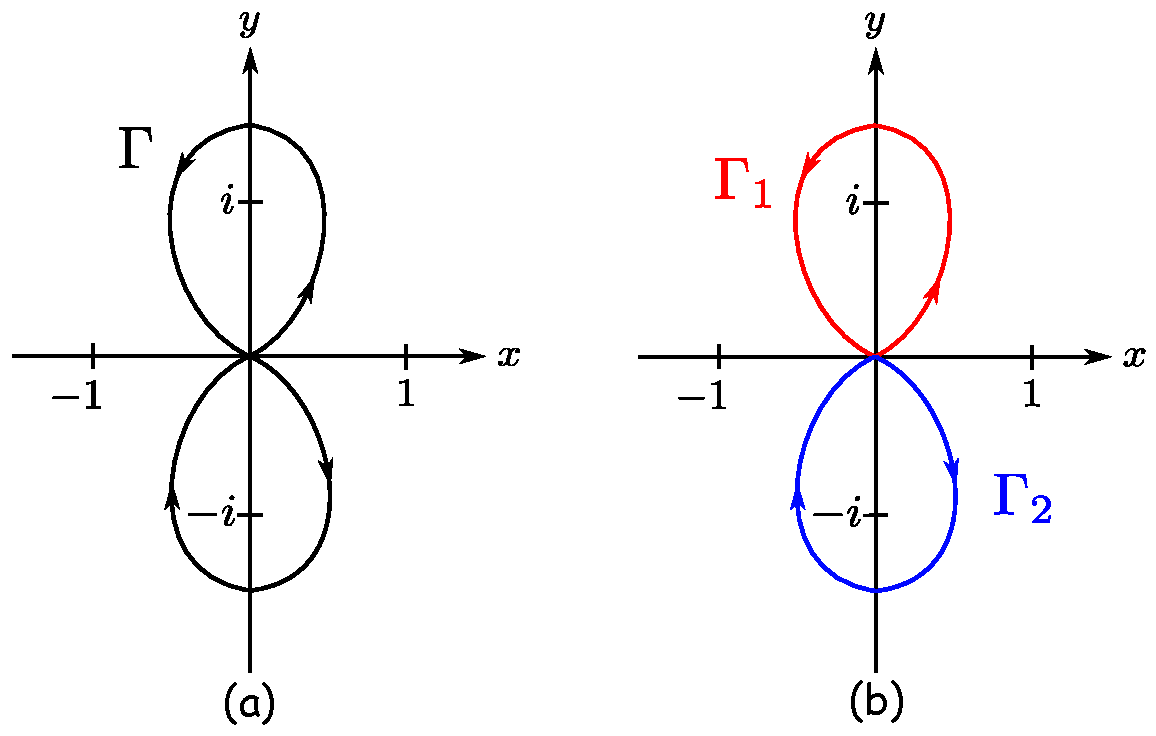
\includegraphics[scale = 0.5]{Figuras/Ejemplo_FIC.pdf}
    \caption{Curva ocho $\Gamma$ en (a) dividida en dos curvas $\Gamma_1$ y $\Gamma_2$ en (b).}
    \label{fig:EjemploFIC}
\end{figure}

Así, 
$$\int_{\Gamma} \frac{z}{(z-i)(z^2+1)} \,dz = \int_{\Gamma_1} \frac{z}{(z-i)(z^2+1)} \,dz + \int_{\Gamma_2} \frac{z}{(z-i)(z^2+1)} \,dz.$$

Ahora podremos usar la fórmula de la integral de Cauchy. Observe que la orientación de las nuevas curvas son distintos: La orientación de $\Gamma_1$ es positiva, mientras que la orientación de $\Gamma_2$ es negativa. Para $\Gamma_1$, aplicamos \ref{FICDerivadas} con $n = 1$, $f(z) = \frac{z}{z+i}$ y $z_0 =i$:
$$\int_{\Gamma_1} \frac{f(z)}{(z-i)^2} \,dz = 2\pi i \frac{d}{dz}\left[ \frac{z}{z+i} \right]_{z=i} = \left. 2\pi i \frac{i}{(z+i)^2} \right|_{z=i} = \frac{\pi}{2}.$$

Para $\Gamma_2$,  aplicamos \ref{FICDerivadas} con $n = 0$, $f(z) = \frac{z}{(z-i)^2}$ y $z_0 = -i$, teniendo en cuenta la orientación de $\Gamma_2$,
$$\int_{\Gamma_2} \frac{f(z)}{z+i} \,dz = \left. - 2\pi i  \frac{z}{(z-i)^2} \right|_{z=-i} = \frac{\pi}{2}.$$

Por lo tanto,
$$\int_{\Gamma} \frac{z}{(z-i)(z^2+1)} \,dz = \pi.$$
\end{ejemplo}

\begin{corolario}\label{corolarioFIC}
Supongamos que $f$ es analítica en un abierto $A$. Entonces $f$ tiene derivadas de todos los órdenes $f',f'',f^{(3)}, f^{(4)},\dots$ las cuales son funciones analíticas en $A$.
\end{corolario}

\begin{proof}
Para $z \in A$, sea $\overline{B}(z,R)$ la bola cerrada contenida en $A$ y $C$ su frontera. Por el teorema \ref{GeneralFIC}, todas las derivadas de $f$ existen en $A\setminus C$, y en particular en el punto $z$ dado.
\end{proof}

\textbf{Observación:} Consideremos la función real $f(x) = x^{5/3}, - \infty < x < \infty$. Sus derivada, $f'(x) = \frac{5}{3} x^{2/3}$, existe y es continua para todo $x \in \mathbb{R}$; sin embargo, $f''(x)$ no existe en $x = 0$. Por lo tanto, este corolario no tiene un análogo para el caso real.

\subsection{Teorema de Morera}

El siguiente teorema es un recíproco parcial del teorema de Cauchy.

\begin{teorema}[de Morera]
Sea $f$ continua en una región $D$ (abierto conexo) y suponga que 
$$\int_{\gamma} f(z) \,dz = 0,$$

para cualquier curva cerrada en $D$. Entonces, $f$ es analítica en $D$, y $f = F\,'$ para alguna función analítica $F$ en $D$.
\end{teorema}

\begin{proof}
De acuerdo al teorema \ref{TFC2}, $f$ admite una primitiva en $D$, es decir, existe una función analítica $F$ tal que $F'(z) = f(z)$ en todo punto de $D$. 

Ahora, de \ref{corolarioFIC}, la derivada de una función analítica es también analítica; y puesto que $f$ es la derivada de $F$, se sigue que $f$ es analítica en $D$.

\end{proof}

\textbf{Observación:} En particular, cuando $D$ es simplemente conexo, tenemos, para la clase de las funciones continuas en $D$, un recíproco del teorema de Cauchy-Goursat para tales dominios.

\section{Módulo máximo}

\subsection{Teorema del módulo máximo}

Partamos con los siguientes ejercicios:

\begin{ejemplo} \label{EjemploTVM}
\ 

\begin{enumerate}
    \item Si $f$ y $\overline{f}$ son analíticas en $D$, entonces $f$ es constante. 
    
    En efecto, sea $f(z) = u(x,y) + iv(x,y)$, entonces $\overline{f(z)} = u(x,y) - iv(x,y)$. Por la condición de ser funciones analíticas, se tiene que se satisfacen las ecuaciones de Cauchy-Riemann, es decir, 
    $$u_x = v_y, \quad u_y = -v_x; \quad u_x = -v_y, \quad u_y = v_x,$$
    
    respectivamente. De aquí, se tiene que las derivadas parciales de $u$ y $v$ son iguales a 0 y, por tanto, constantes.
    
    \item Si $|f(z)| = C$, con $C$ una constante distinta de cero, para todo $z \in D$, y $f$ es analítica, entonces $f = cte$ en $D$.
    
    En efecto, notemos que 
    $$C^2 = |f(z)|^2 = f(z) \overline{f(z)}.$$
    
    Como $f(z) \neq 0$ para todo $z \in D$, se tiene que 
    $$\forall z\in D: ~ \overline{f(z)} = \frac{C^2}{f(z)},$$
    
    la cual analítica. Por lo demostrado en el ejercicio anterior, $f$ es constante en $D$.
\end{enumerate}
\end{ejemplo}

Si $f$ es analítica y no es constante en una región abierta que contiene al disco $|z-z_0| < r_0$ y continua en $|z-z_0| \leq r_0$, entonces, al ser compacto, el módulo de $f$ alcanza su máximo en $|z-z_0| \leq r_0$, pero ¿en qué lugar del disco cerrado alcanza ese máximo y en que lugar no?

\begin{lema} \label{LemaModuloMaximo}
Sea $f$ analítica en un entorno $|z-z_0| < r_0$ de un punto $z_0$. Si $|f(z)| \leq |f(z_0)|$ para todo $z$ de ese entorno, entonces $f(z)$ tiene valor constante $f(z_0)$ sobre ese entorno.
\end{lema}

\begin{proof}
Supongamos que $f$ es analítica en dicho entorno. Sea $z_1$ cualquier punto del entorno distinto del $z_0$, y sea $r = d(z_1,z_0)$. Si consideramos la circunferencia $\gamma(t) = z_0 + re^{it}, 0 \leq t \leq 2\pi$, la fórmula integral de Cauchy nos dice que 
$$f(z_0) = \frac{1}{2\pi} \int_{\gamma} \frac{f(z)}{z-z_0} \,dz.$$

Usando la representación paramétrica de la curva, tenemos
$$
f(z_0) = \frac{1}{2\pi i} \int_0^{2\pi} \frac{f\left(z_0 +  re^{it}\right)}{(z_0 +  re^{it}) - z_0} i r e^{it} \,dt = \frac{1}{2\pi} \int_0^{2\pi} f(z_0 +  re^{it})\,dt.   
$$

Luego,
\begin{equation}
|f(z_0)| \leq \frac{1}{2\pi} \int_0^{2\pi} \left|f\left(z_0 +  re^{it}\right) \right| \,dt.    \label{TVM1}
\end{equation}

Por hipótesis, sabemos que $|f(z)| \leq |f(z_0)|$, para $|z-z_0| < r_0$, entonces
\begin{align}
 \frac{1}{2\pi} \int_0^{2\pi} \left|f\left(z_0 +  re^{it}\right) \right| \,dt &\leq   \frac{1}{2\pi} \int_0^{2\pi} |f(z_0)|\,dt \nonumber \\
 &= \frac{1}{2\pi} |f(z_0)| 2\pi = |f(z_0)|. \label{TVM2}
\end{align}

Combinando \eqref{TVM1} y \eqref{TVM2}, se tiene que 
\begin{align*}
   \frac{1}{2\pi} \int_0^{2\pi} & \left|f\left(z_0 +  re^{it}\right) \right| \,dt \leq |f(z_0)| \leq \frac{1}{2\pi} \int_0^{2\pi} \left|f\left(z_0 +  re^{it}\right) \right| \,dt \\
  &\Rightarrow |f(z_0)| = \frac{1}{2\pi} \int_0^{2\pi} \left|f\left(z_0 +  re^{it}\right) \right| \,dt \\
   &\Leftrightarrow \int_0^{2\pi} \left[ \left| f(z_0 + re^{it}) \right| - |f(z_0)|\right] \,dt = 0. 
\end{align*}

Por la continuidad de la función integrada, tenemos que 
$$|f(z_0 + re^{it})| = |f(z_0)|, \quad 0 \leq t \leq 2\pi.$$

Esto demuestra que $|f(z)| = |f(z_0)|$ para todo $z$ en la circunferencia $|z-z_0| = r$.

Finalmente, al ser $z_1$ un punto arbitrario del entorno, $0 <r <r_0$ también lo es, por tanto $|f(z)| = |f(z_0)|$ sobre el entorno $0 < |z-z_0| < r_0$. Pero sabemos, por el ejemplo \ref{EjemploTVM}, que cuando el módulo de una función analítica es constante en un dominio, la propia función es constante en él. Luego $f(z) = f(z_0)$ en todo punto del entorno.
\end{proof}

\begin{teorema}[del módulo máximo]
Si $f$ es analítica en una región abierta conexa $D$ y existe $z_0 \in D$ tal que $|f(z)| \leq |f(z_0)|$ para todo $z \in D$, entonces $f$ es constante en $D$.
\end{teorema}

\begin{proof}
Probaremos que $|f|$ es constante en $D$, para así concluir que $f$ es constante.

Sea $w \in D$ cualquiera. Como $D$ es conexo, existe un camino poligonal que conecta $z_0$ a $w$, ver figura \ref{fig:ModuloMaximo}. El camino está constituido por una secuencia finita de puntos, en particular, $z_0,z_1, \dots, z_n = w$, pero $D$ es abierto, así que tenemos también una secuencia de bolas abiertas $\{B_0, B_1, \dots, B_n\}$ que satisfacen:
\begin{enumerate}
    \item $B_i$ está contenida en $D$ para $i = 1,2, \dots,n$.
    
    \item $B_i$ contiene al punto $z_{i+1}$ para $i = 0,1, \dots, n-1$.
\end{enumerate}

\begin{figure}[H]
    \centering
    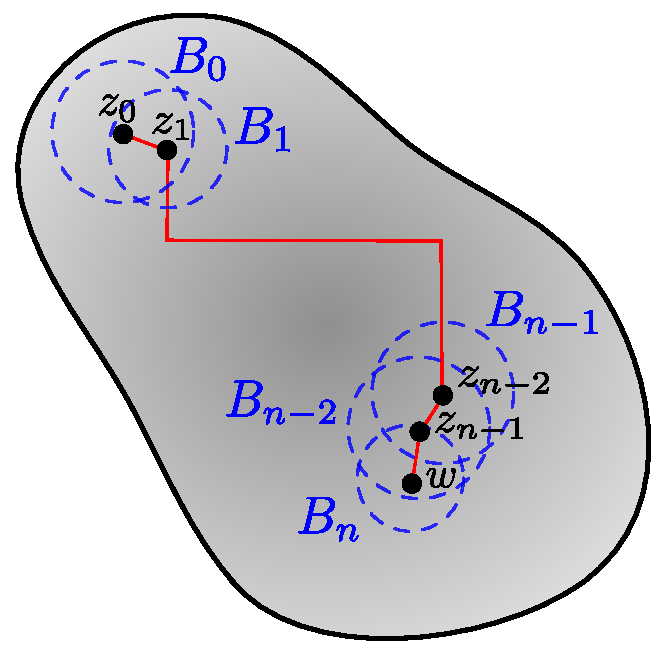
\includegraphics[scale = 0.53]{Figuras/ModuloMaximo.pdf}
    \caption{Demostración del teorema del módulo máximo.}
    \label{fig:ModuloMaximo}
\end{figure}

Debido a que $|f(z)| \leq |f(z_0)|$ para todo $z \in D$,  es el máximo valor de $|f(z)|$ para los $z \in B_0$. Por el lema \ref{LemaModuloMaximo}, $|f(z)|$ es contante en $B_0$. En particular, $|f(z_0)| = |f(z_1)|$, pues $z_1 \in B_0$. Entonces, $|f(z_1)|$ es el máximo valor de $|f(z)|$ en $B_1$. De nuevo, por el lema \ref{LemaModuloMaximo}, $|f(z)|$ es contante en $B_1$. Usando el mismo argumento repetidamente, deducimos que $|f(z)|$ es constante sobre las bolas abiertas $B_0, B_1, \dots, B_n$. En particular, $|f(z_0)| = |f(w)|$. Ahora, como $w$ es arbitrario, concluimos que $|f|$ es constante en $D$. Por lo tanto, $f$ es constante en $D$.  
\end{proof}

El siguiente corolario es consecuencia directa del teorema del módulo máximo y es directamente aplicable a problemas de búsqueda de máximos.

\begin{corolario}
Sea $f$ una función analítica y no constante en una región $D$ y sea $\gamma$ una curva simple cerrada enteramente contenida en $D$. Entonces, el máximo valor alcanzado por $|f(z)|$ en el compacto encerrado por la curva $\gamma$ se alcanza en, precisamente,  $\gamma$.
\end{corolario}

\begin{ejemplo}
Determinar el máximo absoluto de $|f(z)|$ en $|z| \leq 1$ para la función $f(z) = z^2 -3z+2$.
\\

\textbf{Solución:} La función es no constante, analítica en $|z| < 1$ y continua en $|z| = 1$, el teorema del módulo máximo nos dice que el máximo valor de $|f(z)|$ se alcanza en $|z| = 1$. Haciendo $z = x+iy$, tenemos
$$f(z) = f(x+iy) = (x^2 - y^2 -3x+2) + i(2xy-3y).$$

Maximicemos
$$|f(z)|^2 = (x^2 - y^2 -3x+2)^2 + (2xy-3y)^2$$

con la condición $|z| = x^2+y^2 = 1$. Para ello, despejando $y$, $y^2 = 1-x^2$:
\begin{align*}
    |f(z)|^2 &= (2x^2 -3x+1)^2 + (1-x^2)(2x-3)^2 \\
    &= 8x^2 -18x+10, \quad x \in [-1,1].
\end{align*}

Queda como ejercicio para el lector verificar, por medio del teorema de los valores extremos, que el máximo absoluto de $g(x) = 8x^2 -18x+10 $ en $[-1,1]$ es $g(-1) = 36$. Por lo tanto, el máximo módulo de $f$ es
$$|f(-1)| = \sqrt{36} = 6.$$
\end{ejemplo}

\subsection{Teorema de Liouville y el teorema fundamental del Álgebra} 

Dos importantes consecuencias del teorema del módulo máximo son los siguientes teoremas.

\begin{teorema}[de Liouville]
Si $f$ es una función entera y acotada, entonces $f$ es constante.
\end{teorema}

\begin{proof}
Por las hipótesis, existe $M > 0$ tal que
$$\forall z \in \mathbb{C}: ~ |f(z)| \leq M.$$

Luego, para cualquier $z_0 \in \mathbb{C}$ y la circunferencia $C_r: |z-z_0| = r$, se tiene
\begin{align*}
    |f'(z_0)| = \left|\frac{1}{2\pi i} \int_{C_r} \frac{f(z)}{(z-z_0)^2} \,dz \right| &\leq \frac{1}{2\pi} \int_{C_r} \frac{|f(z)|}{|z-z_0|^2} \,|dz| \\
    &\leq \frac{M}{2\pi r^2} \int_{C_r} |dz| \\
    &= \frac{M}{2\pi r^2} 2\pi r = \frac{M}{r}.
\end{align*}

Como $r$ es arbitrario, se concluye que $f'(z_0) = 0$. Pero $z_0$ es, también, arbitario, por tanto
$$f'(z) = 0 \Rightarrow f = cte.$$
\end{proof}

\begin{teorema}[Fundamental del Álgebra]
Cualquier polinomio 
$$P(z) = a_0 + a_1 z + a_2 z^2 + \cdots + a_n z^n,$$

con $a_n \neq 0$ y $n\geq 1$, tiene, al menos, una raíz. Ésto es, existe $z_0 \in \mathbb{C}$ tal que $P(z_0) = 0$.
\end{teorema}

\begin{proof}
Si suponemos que no existe tal raíz, entonces la función
$$f(z) = \frac{1}{P(z)}$$

es una función entera. Mostremos que $f$ es acotada o, equivalentemente, $P$ es acotado.

Notemos que, para cualquier $|z|> 1$, se tiene
\begin{align*}
    |P(z)| &= |z|^{n-1} \left| a_n z + \frac{a_{n-1}}{1} + \frac{a_{n-2}}{z} + \cdots + \frac{a_0}{z^{n-1}} \right| \\
    &\geq |z|^{n-1} \left[ |a_n z|- \frac{|a_{n-1}|}{1} - \frac{|a_{n-2}|}{|z|} - \cdots - \frac{|a_0|}{|z^{n-1}|} \right]
\end{align*}

y si llamamos $a = |a_{n-1}| + \cdots + |a_0|$, entonces
\begin{align*}
  |P(z)|  &\geq |z|^{n-1} \left[ |a_n z|- \frac{|a_{n-1}|}{1} - \frac{|a_{n-2}|}{|z|} - \cdots - \frac{|a_0|}{|z^{n-1}|} \right]  \\
  &\geq |z|^{n-1} \left[ |a_n|\,|z| - |a_{n-1}| - |a_{n-2}| - \cdots - |a_0| \right] \\
  &= |z|^{n-1} \left[ |a_n|\,|z| -a \right].
\end{align*}

Sea $M > 0$ dado y consideremos $K = \max\left\{1, \frac{M+a}{|a_n|} \right\}$, luego para $|z| > K$, se tiene que
$$|P(z)| \geq  |z|^{n-1} \left[ |a_n|\,|z| -a \right] >  \left[ |a_n|\, \frac{M+a}{|a_n|} -a \right] = M $$

de donde se concluye que
$$|z| > K \Rightarrow |f(z)| = \frac{1}{|P(z)|} < \frac{1}{M}.$$

Ahora, $f$ es continua en la bola cerrada de centro $0$ y radio $K$, luego $f$ es acotada aquí por algún $N > 0$. Así,
$$\forall z \in \mathbb{C}: ~ |f(z)| \leq \max\left\{ N,\frac{1}{M} \right\}.$$

Por el teorema de Liouville, $f$ es constante, lo que implica que $P$ es constante. Ésto es una contradicción, ya que del hecho que $a_n \neq 0$, $P$ no es constante. Tal contradicción viene de suponer que $f(z) \neq 0$, para todo $z \in \mathbb{C}$. De esta manera, hemos probado que existe $z_0 \in \mathbb{C}$ tal que
$$f(z_0) = 0.$$
\end{proof}


\chapter{Series}

\section{Sucesiones numéricas}

\begin{defi}
Una \textbf{sucesión} de números complejos es una función del tipo
$$f: \mathbb{N} \rightarrow \mathbb{C}, \quad n \mapsto f(z) = z_n.$$
\end{defi}

\textbf{Observación:} Su recorrido es 
$$\{z_n : n \in \mathbb{N}\} = \{z_1, z_2, \dots, z_n\}.$$

Con el fin de simplificar las notaciones, denotaremos una sucesión simplemente por 
$$\{z_n\}_{n\in \mathbb{N}}, ~ \{z_n\}_{n=1}^{\infty}, ~ \{z_n\}_{n=m}^{\infty}, ~ etc.$$

\begin{defi}
Se dice que una sucesión $\{z_n\}_{n=1}^{\infty}$ \textbf{converge} a $z \in \mathbb{C}$ si
$$(\forall \varepsilon > 0)(\exists N \in \mathbb{N})(\forall n: ~ n \geq N \Rightarrow |z_n - z| < \varepsilon).$$

Ésto se denotará por
$$\lim_{n\to +\infty} z_n = z$$

y $z$ se llamará límite de la sucesión $\{z_n\}_{n=1}^{\infty}$. Si no existe tal $z \in \mathbb{C}$ diremos que $\{z_n\}_{n=1}^{\infty}$ \textbf{diverge}.
\end{defi}

\begin{figure}[H]
    \centering
    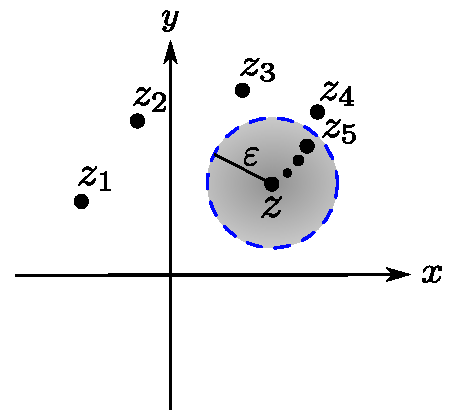
\includegraphics[scale = 0.7]{Figuras/ConvergenciaSucesion.pdf}
    \caption{Sucesión $\{z_n\}_{n\in \mathbb{N}}$ convergiendo a $z$.}
    \label{fig:Sucesion}
\end{figure}

Para sucesiones que convergen a cero, es fácil de ver que
$$\lim_{n\to + \infty} z_n = 0 \Leftrightarrow \lim_{n \to + \infty} |z_n| = 0.$$

Note que las definiciones son similares al de las sucesiones reales, por tanto se omitirán las demostraciones que sean similares al caso real.

\begin{propo}
Si el límite de una sucesión compleja existe, entonces éste es único.
\end{propo}

\begin{teorema} \label{SucesionCom-Re}
Sea $\{z_n\}_{n \in \mathbb{N}}$ una sucesión de números complejos tal que $z_n = x_n + iy_n$, donde $x_n=Re(z_n)$ e $y_n = Im(z_n)$. Entonces, para $z = x + iy$, tenemos
$$\lim_{n\to + \infty} z_n = z \Leftrightarrow \lim_{n\to + \infty} x_n = x ~\wedge~ \lim_{n\to + \infty} y_n = y.$$
\end{teorema}

\begin{proof}
Supongamos que $\lim\limits_{n\to + \infty} z_n = z$, entonces dado $\varepsilon >0 $, $\exists N \in \mathbb{N}$ tal que 
$$\forall n: ~ n \geq N \Rightarrow |z_n-z| = |(x_n-x) + i (y_n-y)| < \varepsilon.$$

Usando el mismo $N \in \mathbb{N}$, se verifica:
\begin{align*}
    \forall n:~ n \geq N &\Rightarrow |x_n-x| \leq  |(x_n-x) + i (y_n-y)| < \varepsilon, \\
    \forall n:~ n \geq N & \Rightarrow |y_n-y| \leq  |(x_n-x) + i (y_n-y)| < \varepsilon.
\end{align*}

Por lo tanto,
$$\lim_{n\to + \infty} x_n = x \wedge \lim_{n\to + \infty} y_n = y.$$

Por otro lado, supongamos que $\lim\limits_{n\to + \infty} x_n = x$ y $\lim\limits_{n\to + \infty} y_n = y$, entonces dado $\varepsilon > 0$, $\exists N_1, N_2 \in \mathbb{N}$ tales que
\begin{align*}
    \forall n:~ n \geq N_1 &\Rightarrow |x_n-x|  < \frac{\varepsilon}{2}, \\
    \forall n:~ n \geq N_2 &\Rightarrow |y_n-y| < \frac{\varepsilon}{2}.
\end{align*}

Eligiendo $N = \max\{N_1, N_2\}$, se verifica:
\begin{align*}
    \forall n: ~ n\geq N \Rightarrow |z_n-z| &=  |(x_n-x) + i (y_n-y)| \\
    &\leq |x_n-x| + |y_n-y| \\
    &< \frac{\varepsilon}{2} + \frac{\varepsilon}{2} = \varepsilon.
\end{align*}

Por lo tanto, 
$$\lim_{n\to + \infty} z_n = z.$$
\end{proof}

\begin{ejemplo}
Estudiar el comportamiento de la sucesión $\{(i)^n\}_{n \in \mathbb{N}}$.
\\

\textbf{Solución:} Consideremos las siguientes subsucesiones: $\left\{ (i)^{4k-2}\right\}_{k \in \mathbb{N}}$ y $\left\{ (i)^{4k}\right\}_{k \in \mathbb{N}}$. Luego,
\begin{align*}
    \lim_{k \to + \infty} (i)^{4k-2} &= \lim_{k \to + \infty} (-1) = -1, \\
    \lim_{k \to + \infty} (i)^{4k} &= \lim_{k \to + \infty} 1 = 1.
\end{align*}

Como $\lim\limits_{k \to + \infty} i^{4k-2} \neq \lim\limits_{k \to + \infty} i^{4k}$, la sucesión $\{(i)^n\}_{n \in \mathbb{N}}$ diverge.
\end{ejemplo}

\begin{defi}
Una sucesión de números complejos $\{z_n\}_{n=1}^{\infty}$ se dice que es \textbf{acotada} si existe $M > 0$ tal que 
$$\forall n \in \mathbb{N}: ~ |z_n| \leq M.$$
\end{defi}

\begin{teorema}
Toda sucesión de números complejos convergente es acotada.
\end{teorema}

\textbf{Observación:} El recíproco es falso, pues la sucesión $\{(i)^n\}_{n \in \mathbb{N}}$ es acotada pero no converge.

\begin{teorema}
Sean $\{z_n\}_{n\in \mathbb{N}}$ y $\{w_n\}_{n\in \mathbb{N}}$  sucesiones de números complejos.
\begin{itemize}
    \item[(i)] Si $\lim\limits_{n\to + \infty} z_n = 0$ y $|w_n| \leq |z_n|$ para todo $n \geq N_0 \in \mathbb{N}$. Entonces, $\lim\limits_{n\to + \infty} w_n = 0$.
    
    \item[(ii)] Si  $\lim\limits_{n\to + \infty} z_n = 0$ y $\{w_n\}_{n\in \mathbb{N}}$ es acotada, entonces  $\lim\limits_{n\to + \infty} z_n w_n = 0$.
\end{itemize}
\end{teorema}

\begin{teorema}[Álgebra de límites]
Sean $\{z_n\}_{n\in \mathbb{N}}$ y $\{w_n\}_{n\in \mathbb{N}}$  dos sucesiones de números complejos convergentes y $\alpha,\beta \in \mathbb{C}$. Entonces
\begin{itemize}
\item[(i)] $$\lim\limits_{n \to + \infty} (\alpha z_n + \beta w_n ) = \alpha \lim\limits_{n\to + \infty} z_n + \beta \lim\limits_{n\to + \infty} w_n;$$

\item[(ii)] $$\lim\limits_{n \to + \infty} ( z_n w_n) = \left( \lim\limits_{n\to + \infty} z_n\right) \cdot \left(\lim\limits_{n\to + \infty} w_n \right);$$

\item[(iii)] $$\lim\limits_{n \to + \infty} \frac{z_n}{w_n} = \frac{\lim\limits_{n\to + \infty} z_n}{\lim\limits_{n\to + \infty} w_n}, \quad \mbox{cuando} ~\lim\limits_{n\to + \infty} w_n \neq 0;$$

\item[(iv)] $$\lim\limits_{n \to + \infty} \overline{z_n} = \overline{\lim\limits_{n\to + \infty} z_n};$$

\item[(v)] $$\lim\limits_{n\to + \infty} |z_n| = \left| \lim\limits_{n\to + \infty} z_n\right|.$$
\end{itemize}
\end{teorema}

\begin{ejemplo} \label{EjemploSucesion}
Muestre que
$$\lim_{n\to + \infty} z^n = \left\{ \begin{array}{cl}
    0,& \mbox{si} ~ |z| < 1  \\
    1, &  \mbox{si} ~ z = 1 \\
    diverge, &\mbox{si} ~ |z| = 1 \wedge z \neq 1 \\
    diverge, &\mbox{si} ~ |z| > 1
\end{array} \right. .$$

\textbf{Solución:} Recordemos que para un número real $r \geq 0$, tenemos
$$\lim_{n\to + \infty} r^n = \left\{ \begin{array}{cl}
    0,& \mbox{si} ~ 0\leq r < 1  \\
    1, &  \mbox{si} ~ r = 1 \\
    \infty, &\mbox{si} ~ r > 1
\end{array} \right. .$$


En consecuencia, para un número complejo $|z| < 1$, tenemos 
$$\lim_{n\to + \infty} |z|^n = \lim_{n\to + \infty} |z^n| =   0 \Rightarrow  \lim_{n\to + \infty} z^n = 0.$$

Para $|z| > 1$, tenemos que 
$$\lim_{n\to + \infty} |z|^n = + \infty,$$

ésto es, $\{z_n\}_{n = 1}^{\infty}$ no es acotada. Luego, no converge. 

Ahora, para $|z| = 1$, es trivial que si $z = 1$ la sucesión converge. El caso $|z| = 1$, $z\neq 1$, no es tan simple, pues la sucesión está acotada. Supongamos que la serie converge, es decir,
$$\lim_{n\to + \infty} z^n = L \in \mathbb{C} \Rightarrow |L| = \lim_{n\to + \infty} |z|^n = 1,$$

así $L \neq 0$. Además, si $z^n \to L$, entonces $z^{n+1} \to L$ cuando $n\to + \infty$. Pero 
$$L = \lim_{n\to + \infty} z^{n+1} = \lim_{n\to + \infty} z^{n}z = Lz.$$

Dividiendo por $L$, deducimos que $z = 1$, lo cual es una contradicción, pues $|z| =1$ con $z \neq 1$. Por lo tanto, la sucesión diverge.
\end{ejemplo}

Antes de finalizar la sección, estudiemos la completitud de $\mathbb{C}$, ésto es, si las \textit{sucesiones de Cauchy} convergen. Para ello, recordemos que son estas sucesiones.

\begin{defi}
Una sucesión $\{z_n\}_{n=1}^{\infty}$ se dice que es una \textbf{sucesión de Cauchy} si para cada $\varepsilon > 0$, existe $N \in \mathbb{N}$ tal que
$$\forall n,m:~ n,m \geq N \Rightarrow |z_n-z_m| < \varepsilon.$$
\end{defi}

Utilizando como hecho la completitud de los reales, podemos probar el siguiente teorema.

\begin{teorema}
Una sucesión $\{z_n\}_{n=1}^{\infty}$ de números complejos converge si y sólo si es una sucesión de Cauchy.
\end{teorema}

\begin{proof}
Supongamos que $\{z_n\}_{n=1}^{\infty}$ converge a $z \in \mathbb{C}$, entonces dado $\varepsilon >0$, $\exists N \in \mathbb{N}$ tal que
$$\forall n:~ n \geq N ~\Rightarrow~ |z_n - z| < \frac{\varepsilon}{2}.$$

Sean $n,m \geq N$, se cumple
$$|z_n - z_m| = |(z_n - z) + (z - z_m)| \leq |z_n -z| + |z_m - z| < \varepsilon.$$

Por lo tanto, $\{z_n\}_{n=1}^{\infty}$ es de Cauchy, probando así la implicancia hacia la derecha.
\\

Por otro lado, supongamos que $\{z_n\}_{n=1}^{\infty}$ es una sucesión de Cauchy, entonces
$$(\forall \varepsilon > 0)(\exists N \in \mathbb{N})(\forall n,m: ~ n,m \geq N ~\Rightarrow~ |z_n-z_m| < \varepsilon)$$

Si $z_n = x_n + iy_n$, entonces
$$|x_n - x_m| < \varepsilon ~\wedge~ |y_n - y_m| < \varepsilon, \quad \forall n,m \geq N.$$

Ésto es, las sucesiones $\{x_n\}_{n=1}^{\infty}$ y  $\{y_n\}_{n=1}^{\infty}$  son de Cauchy en $\mathbb{R}$ y en consecuencia convergen. Finalmente, por el teorema \ref{SucesionCom-Re}, la sucesión $\{z_n\}_{n=1}^{\infty}$ converge, probando así la implicancia hacia la izquierda.
\end{proof}

\section{Series numéricas}

\begin{defi}
Sea $\{z_n\}_{n=1}^{\infty}$ una sucesión de números complejos. Se define la sucesión de \textbf{sumas parciales}  $\{s_n\}_{n=1}^{\infty}$ por 
\begin{align*}
    s_1 &= z_1 \\
    s_2 &= s_1 + z_2 = z_1+ z_2 \\
    s_3 &= s_2 + z_3 = z_1 + z_2 + z_3 \\
    &~\,\vdots \\
    s_n &= s_{n-1} + z_n = z_1 + z_2 + z_3 + \cdots + z_n.
\end{align*}

Esta nueva sucesión recibe el nombre de \textbf{serie} de término general $z_n$ y se denota
$$\sum_{n=1}^{\infty} z_n.$$

Si la sucesión de sumas parciales $\{s_n\}_{n=1}^{\infty}$ converge al valor $S$, se dice que la serie es convergente y se escribe
$$\sum_{n=1}^{\infty} z_n = S.$$

El número $S$ se llama \textbf{suma} de la serie. Si   $\{s_n\}_{n=1}^{\infty}$ diverge, se dice que la serie diverge.
\end{defi}

\begin{ejemplo} \label{SerieGeo}
Muestre que si $|z| < 1$, la \textbf{serie geométrica} $\sum\limits_{n=0}^{\infty} z^n$ converge y
$$\sum_{n=0}^{\infty} z^n = \frac{1}{1-z}.$$

Muestre también que la serie diverge para los otros valores de $z$.
\\

\textbf{Solución:} 

Para $z=1$, la $n$-ésima suma parcial es $s_n = n$ y por tanto la serie diverge.

Para $z\neq 1$, la $n$-ésima suma parcial es
\begin{equation}
    s_n = \sum_{k=0}^n z^k = 1 + z +z^2 + \cdots + z^n. \label{Geometrica1}
\end{equation}

Multiplicando por $z$:
\begin{equation}
    z s_n = \sum_{k=0}^n z^{k+1} = z + z^2  + \cdots + z^n + z^{n+1}. \label{Geometrica2}
\end{equation}

Entonces, tomando la diferencia entre \eqref{Geometrica1} y \eqref{Geometrica2}, tenemos
$$(1-z) s_n = \sum_{k=0}^n [z^k - z^{k+1}] = 1 - z^{n+1} ~\Rightarrow~ s_n = \frac{1-z^{n+1}}{1-z}.$$

Por el ejemplo \ref{EjemploSucesion}, tenemos que $\{z^{n+1}\}_{n=0}^{\infty}$ converge a 0 si $|z|<1$ y diverge si $|z| > 1$ o $|z|=1$ y $z \neq 1$. Esto implica que
$$\sum_{n=0}^{\infty} z^n = \frac{1}{1-z}, \quad |z| <1.$$
\end{ejemplo}
\newpage

Al igual que en el caso de las sucesiones, se omitirán las demostraciones que son análogas al caso real.

\begin{teorema} \label{SerieCom-Re}
Sea $\sum\limits_{n=1}^{\infty} z_n$ una serie de números complejos tal que $z_n = x_n + iy_n$, donde $x_n=Re(z_n)$ e $y_n = Im(z_n)$. Entonces, para $S = x + iy$, tenemos
$$\sum_{n=1}^{\infty} z_n = S \Leftrightarrow \sum_{n=1}^{\infty} x_n = x ~\wedge~ \sum_{n=1}^{\infty} y_n = y.$$
\end{teorema}

\begin{proof}
Sea $S_n$ la $n$-ésima suma parcial de la serie $\sum\limits_{n=1}^{\infty} z_n$, observemos que
$$S_n = X_n + i Y_n,$$

donde
$$X_n = \sum_{k=1}^n x_n ~~\mbox{y}~~ Y_n = \sum_{k=1}^n y_n.$$

Ahora, por el teorema \ref{SucesionCom-Re}, 
$$\lim_{n \to + \infty} S_n = S \Leftrightarrow \lim_{n \to \infty} X_n = x ~\wedge~ \lim_{n \to \infty} Y_n = y.$$

Como $X_n$ e $Y_n$ son las $n$-ésimas sumas parciales de las series $\sum\limits_{n=1}^{\infty} x_n$ y $\sum\limits_{n=1}^{\infty} y_n$, respectivamente. Queda demostrado el teorema.

\end{proof}

\begin{teorema}\label{AlgebraSeries}
Si $\sum\limits_{n=1}^{\infty} z_n$ y $\sum\limits_{n=1}^{\infty} w_n$ son series de números complejos convergentes, y $\alpha,\beta \in \mathbb{C}$. Entonces,
\begin{itemize}
    \item[(i)] $\sum\limits_{n=1}^{\infty} (\alpha z_n + \beta w_n) = \alpha \sum\limits_{n=1}^{\infty} z_n + \beta \sum\limits_{n=1}^{\infty} w_n;$
    
    \item[(ii)] $\overline{\sum\limits_{n=1}^{\infty} z_n} =  \sum\limits_{n=1}^{\infty} \overline{z_n};$
    
    \item[(iii)] $Re\left(\sum\limits_{n=1}^{\infty} z_n\right) =\sum\limits_{n=1}^{\infty} Re(z_n)$ y $Im\left(\sum\limits_{n=1}^{\infty} z_n\right) =\sum\limits_{n=1}^{\infty} Im(z_n)$
\end{itemize}
\end{teorema}

En el siguiente ejemplo se ilustra como podemos usar series complejas para determinar una serie real.

\begin{ejemplo}
Mostrar que 
$$\sum_{n=0}^{\infty} \frac{\cos(n\theta)}{2^n}$$

converge para todo $\theta$ y encontrar la suma.
\\

\textbf{Solución:} Notemos que $\cos(n\theta)$ es la parte real de $(\cos\theta + i \sin \theta)^n$, entonces la serie dada es la parte real de la serie geométrica
$$\sum_{n=0}^{\infty} z^n, \quad \mbox{donde} ~ z = \frac{1}{2}(\cos \theta + i \sin \theta).$$

Como $|z| = 1/2 < 1$, tenemos que la serie converge y
\begin{align*}
 \sum_{n=0}^{\infty} z^n = \frac{1}{1-z} &= \frac{1}{\left(1 - \frac{1}{2} \cos \theta \right) - \frac{i}{2} \sin \theta } \cdot \frac{\left(1 - \frac{1}{2} \cos \theta \right) + \frac{i}{2} \sin \theta}{\left(1 - \frac{1}{2} \cos \theta \right) + \frac{i}{2} \sin \theta} \\
 &= \frac{1 - \frac{1}{2} \cos \theta  + \frac{i}{2} \sin \theta}{\left(1 - \frac{1}{2} \cos \theta \right)^2 + \left(\frac{1}{2} \sin \theta\right)^2} \\
 &= \frac{4-2\cos\theta+2i\sin\theta}{5-4\cos \theta}.
\end{align*}

Tomando las partes reales y usando el teorema \ref{AlgebraSeries} (iii), obtenemos 
$$\sum_{n=0}^{\infty} \frac{\cos(n\theta)}{2^n} = Re\left( \frac{4-2\cos\theta+2i\sin\theta}{5-4\cos \theta}\right) = \frac{4-2\cos \theta}{5-4\cos \theta}, \quad \forall\theta\in \mathbb{R}.$$
\end{ejemplo}

\begin{propo}
Si la serie $\sum\limits_{n=1}^{\infty} z_n$ es convergente, entonces $\lim\limits_{n\to + \infty} z_n = 0.$
\end{propo}

En la práctica, el contrarrecíproco es más útil:
$$\lim_{n\to + \infty} z_n \neq 0 ~\Rightarrow~ \sum_{n=1}^{\infty} z_n ~ \mbox{es divergente}.$$

\begin{defi}
Sea $\sum\limits_{n=1}^{\infty } z_n$ una serie de números complejos. Diremos que  $\sum\limits_{n=1}^{\infty } z_n$ \textbf{converge absolutamente} si $\sum\limits_{n=1}^{\infty} |z_n|$ converge. 
\end{defi}

\begin{teorema} \label{CVAbsoluta}
Las series absolutamente convergentes son convergentes, es decir, para $z_n \in \mathbb{C}$,
$$\sum_{n=1}^{\infty} |z_n| < \infty \Rightarrow \sum_{n=1}^{\infty} z_n ~\mbox{converge}.$$
\end{teorema}

\begin{proof}
Si $z_n = x_n + iy_n$, por hipótesis, la serie
$$\sum_{n=1}^{\infty} |z_n| = \sum_{n=1}^{\infty} \sqrt{x_n^2 + y_n^2}$$

de números reales converge. Como
$$|x_n| \leq \sqrt{x_n^2 + y_n^2} ~~\mbox{y}~~ |y_n| \leq \sqrt{x_n^2 + y_n^2},$$

usando el criterio de comparación directa real, las dos series
$$\sum_{n=1}^{\infty} |x_n| ~~\mbox{y}~~ \sum_{n=1}^{\infty} |y_n|$$

convergen. Además, ya que la convergencia absoluta de una serie de números reales implica la convergencia de la propia serie, se sigue que 
$$\sum_{n=1}^{\infty} x_n  ~~\mbox{y}~~ \sum_{n=1}^{\infty} y_n$$

convergen y, en consecuencia, también lo hace $\sum\limits_{n=1}^{\infty} z_n$.
\end{proof}

La importancia de este teorema radica en que al ser $\sum\limits_{n=1}^{\infty} |z_n|$ una serie real, los criterios usuales para series reales que conocemos del cálculo, pueden ser utilizados. 

\begin{teorema}
Supongamos que $z_n$ son números complejos, $a_n$ son números reales, $|z_n| \leq  a_n$ para todo $n \geq N_0 \in \mathbb{N}$, y $\sum\limits_{n=1}^{\infty} a_n$ es convergente. Entonces, $\sum\limits_{n=1}^{\infty} z_n$ es absolutamente convergente.
\end{teorema}

\begin{proof}
Directo del criterio de comparación directa para series reales y el teorema \ref{CVAbsoluta}.
\end{proof}

\begin{ejemplo}
Estudie la convergencia de la serie
$$\sum_{n=0}^{\infty} \frac{2\cos(n\theta) + 2i \sin(n\theta)}{n^2+3}.$$

\textbf{Solución:} Notemos que
$$\forall n \in \mathbb{N}: ~ \left| \frac{2\cos(n\theta) + 2i \sin(n\theta)}{n^2+3} \right| = \frac{2|\cos(n\theta) + i \sin(n\theta)|}{n^2+3} \leq \frac{2}{n^2+3} \leq \frac{2}{n^2}.$$

Como la serie $\sum\limits_{n=1}^{\infty} \frac{2}{n^2}$ converge, la serie
$$\sum_{n=0}^{\infty} \frac{2\cos(n\theta) + 2i \sin(n\theta)}{n^2+3} ~ \mbox{converge}.$$
\end{ejemplo}

Los criterios del cociente y de la raíz también pueden ser aplicados como se ilustra en los siguientes teoremas.

\begin{teorema}[Criterio del cociente]
Sea $\{z_n\}_{n=1}^{\infty}$ una sucesión de números complejos no nulos y 
$$L = \lim_{n \to + \infty} \left|\frac{z_{n+1}}{z_n} \right|.$$

Entonces,
\begin{itemize}
\item[i)] $0\leq L < 1 ~\Rightarrow~ \sum\limits_{n=1}^{\infty} z_n$ es absolutamente convergente.

\item[ii)] $L > 1 ~\Rightarrow~ \sum\limits_{n=1}^{\infty} z_n $ es divergente. \qquad (también para $L = + \infty$)

\item[iii)] Para $L = 1$, el criterio no proporciona información.
\end{itemize} 
\end{teorema}

\begin{ejemplo}
La serie
$$\sum_{n=0}^{\infty} \frac{z^n}{n!}$$

converge absolutamente para todo $z \in \mathbb{C}$. En efecto, la serie claramente converge si $z = 0$. Para $z \neq 0$,
$$L = \lim_{n\to + \infty} \left| \frac{z^{n+1}n!}{z^n (n+1)!} \right| = \lim_{n\to + \infty} \frac{|z|}{n+1} = 0.$$

Como $L < 1$, la serie converge absolutamente por el criterio del cociente.
\end{ejemplo}

\begin{teorema}[Criterio de la raíz]
Sea $\{z_n\}_{n=1}^{\infty}$ una sucesión de números complejos y 
$$L = \lim_{n \to + \infty} \sqrt[n]{|z_n|}.$$

Entonces,
\begin{itemize}
\item[i)] $0\leq L < 1 ~\Rightarrow~ \sum\limits_{n=1}^{\infty} z_n$ es absolutamente convergente.

\item[ii)] $L > 1 ~\Rightarrow~ \sum\limits_{n=1}^{\infty} z_n $ es divergente. \qquad (también para $L = + \infty$)

\item[iii)] Para $L = 1$, el criterio no proporciona información.
\end{itemize} 
\end{teorema}

\begin{ejemplo}
Estudie la convergencia de 
$$\sum_{n=0}^{\infty} \frac{z^n}{(n+1)^n}.$$

\textbf{Solución:} Usando el criterio de la raíz, tenemos
$$L = \lim_{n\to + \infty} \left| \frac{z^n}{(n+1)^n} \right|^{\frac{1}{n}}  = \lim_{n\to + \infty} \frac{|z|}{n+1} = 0.$$

Como $L < 1$, la serie converge absolutamente para todo $z \in \mathbb{C}$.
\end{ejemplo}

\section{Sucesiones y series de funciones}

En las secciones previas hemos considerado sucesiones y series de números complejos. Ahora nos centraremos en sucesiones y series de funciones.

\begin{defi}[Sucesión de funciones]
Sea $\{f_n\}_{n \in \mathbb{N}}$ una sucesión de funciones 
$$f_n: D \subseteq \mathbb{C} \longrightarrow \mathbb{C}.$$

y considere $f: D \subseteq \mathbb{C} \longrightarrow \mathbb{C}$.

\begin{enumerate}
    \item Diremos que $\{f_n\}_{n \in \mathbb{N}}$ \textbf{converge puntualmente} a $f$ si dado $z \in D$ se tiene que la sucesión de números complejos $\{f_n(z)\}_{n \in \mathbb{N}}$ converge a $f(z)$ donde $f$ se llama la \textbf{función límite} de $\{f_n\}_{n \in \mathbb{N}}$, matemáticamente:
    $$(\forall z \in D)(\forall \varepsilon > 0)(\exists N(z,\varepsilon) \in \mathbb{N})(n \geq N ~\Rightarrow~ |f_n(z) - f(z)| < \varepsilon).$$
    
    \textbf{Notación:} $\lim\limits_{n \to + \infty} f_n(z) = f(z)$.
    
    \item  Diremos que $\{f_n\}_{n \in \mathbb{N}}$ \textbf{converge uniformemente} a $f$ si 
     $$(\forall \varepsilon > 0)(\exists N(\varepsilon) \in \mathbb{N})(n \geq N ~\wedge~  z \in D ~\Rightarrow~ |f_n(z) - f(z)| < \varepsilon).$$
     
     \textbf{Notación:} $\lim\limits_{n \to + \infty} f_n(z) = f(z) ~[uniforme]$.
\end{enumerate}
\end{defi}

\textbf{Observación:} Es fácil de ver que si $\{f_n\}_{n\in \mathbb{N}}$ converge uniformemente a $f$, entonces $\{f_n\}_{n\in \mathbb{N}}$ converge puntualmente a $f$.

\begin{defi}[Serie de funciones]
Sea $\{f_n\}_{n \in \mathbb{N}}$ una sucesión de funciones
$$f_n: D \subseteq \mathbb{C} \longrightarrow \mathbb{C}.$$

Sea $F_n = \sum\limits_{k=1}^n f_k$. Se llama \textbf{serie de funciones} a la sucesión de sumas parciales $\{F_n\}_{n\in\mathbb{N}}$ y se denota por $\sum\limits_{n=1}^{\infty} f_n$.

\begin{enumerate}
    \item La serie $\sum\limits_{n=1}^{\infty} f_n$ converge (puntualmente) a $F$ si y solamente si $\{F_n\}_{n \in \mathbb{N}}$ converge puntualmente a $F$ sobre $D$.
    
    \textbf{Notación:} 
    $$\sum_{n=1}^{\infty} f_n = F = \lim_{n\to + \infty} \sum_{k=1}^n f_k.$$
    
    \item La serie $\sum\limits_{n=1}^{\infty} f_n$ converge uniformemente a $F$  sobre $D$ si y solamente si $\{F_n\}_{n \in \mathbb{N}}$ converge uniformemente a $F$ sobre $D$.
    
    \textbf{Notación:} 
    $$\sum_{n=1}^{\infty} f_n = F ~[uniforme].$$
    
\end{enumerate}
\end{defi}

En general, la convergencia puntual no preserva propiedades deseadas de las funciones $f_n$. Por ejemplo, el límite de funciones continuas puede no ser continua (ver ejemplo \ref{EjContinuidadUnifor}); y el límite de funciones analíticas pueden no ser analíticas. Estas propiedades son preservadas, sin embargo, por una convergencia más fuerte como lo es la convergencia uniforme.

\begin{ejemplo} \label{EjContinuidadUnifor}
Sea $f_n(x) = x^n, 0 \leq x \leq 1$. La sucesión $\{f_n\}$ converge puntualmente en el intervalo $[0,1]$,

\begin{figure}[H]
\begin{center}
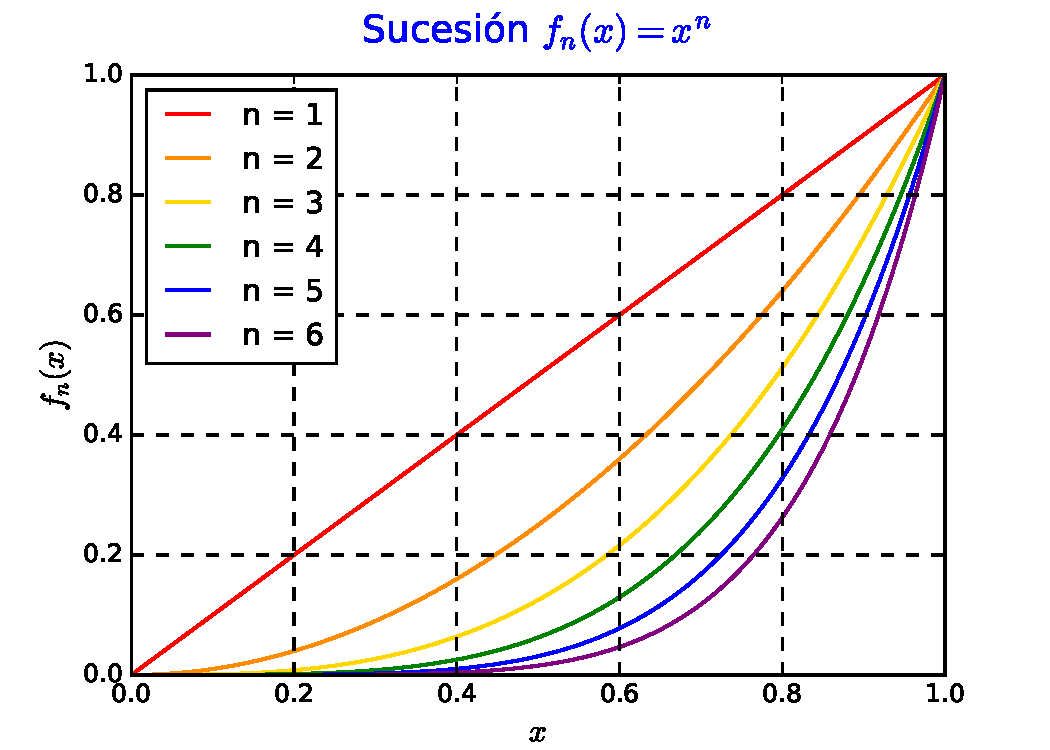
\includegraphics[scale=0.6]{Figuras/SucesionPolinomios.pdf}
\caption{Sucesión de polinomios $x^n, 0 \leq x \leq 1$ para $n = 1,2, \dots,6$.}
\end{center}
\end{figure}
\vspace{-0.7cm}

 y su función límite viene dada por
$$f(x) = \lim_{n\to + \infty} x^n = \left\{ \begin{array}{cl}
0,& 0 \leq x < 1 \\
1 ,& x = 1
\end{array} \right. .$$

Note que a pesar que cada término de la sucesión es continuo en $[0,1]$, $f$ no es continua en $x = 1$.
\end{ejemplo}

\begin{teorema}\label{UniformeContinuo}
Si $\{f_n\}_{n=1}^{\infty}$ es una sucesión de funciones complejas que converge uniformemente a $f$ en un dominio $D$ y cada función $f_n$ es continua en cada punto $z_0 \in D$, entonces la función límite $f$ también es continua en $z_0$.
\end{teorema}

\begin{proof}
Por convergencia uniforme, dado $\varepsilon > 0$, $\exists N \in \mathbb{N}$ tal que
$$n \geq N   ~\wedge~  z \in D ~\Rightarrow~ |f_n(z) - f(z)| < \frac{\varepsilon}{3}.$$

Además, por la continuidad de $f_N$ en $z_0$, existe $\delta = \delta (\varepsilon, N, z_0)$ tal que
$$\forall z: ~ 0 < |z-z_0| < \delta, z \in D ~\Rightarrow~ |f_N(z) - f_N(z_0)| < \frac{\varepsilon}{3}.$$

Por lo tanto,
\begin{align*}
\forall z:~ 0 < |z-z_0| < \delta, z \in D &\Rightarrow |f(z) - f(z_0)| \\
&= |f(z) - f_N(z) + f_N(z) - f_N(z_0) + f_N(z_0) - f(z_0)| \\
&\leq |f(z) - f_N(z)| + |f_N(z) - f_N(z_0)| + |f_N(z_0) - f(z_0)| \\
&< \frac{\varepsilon}{3} + \frac{\varepsilon}{3} + \frac{\varepsilon}{3} = \varepsilon.
\end{align*}
\end{proof}

A veces usamos el teorema \ref{UniformeContinuo} para probar que una sucesión no converge uniformemente.

\begin{ejemplo}
Una sucesión de funciones es definida en el disco unitario por \footnote{Para una visión gráfica puede acceder al siguiente archivo \href{https://www.geogebra.org/m/bedmcah3}{Geogebra}.}
$$f_n(z) =  \left\{ \begin{array}{cl}
n|z|,& \mbox{si}~~ |z| \leq \frac{1}{n} \\
1 ,& \mbox{si}~~  \frac{1}{n} < |z| \leq 1
\end{array} \right. .$$

¿La sucesión converge uniformemente para $|z| \leq 1$?
\\

\textbf{Solución:} Es claro que cada $f_n$ es continua en $\{z \in \mathbb{C} : |z| \leq 1\}$ y
$$\lim_{n \to + \infty} f_n(z) =  \left\{ \begin{array}{cl}
1,& \mbox{si}~~ 0 < |z| \leq 1 \\
0 ,& \mbox{si}~~  z = 0
\end{array} \right. .$$

Dado que la función límite no es continua en $z =0$, podemos concluir, a partir del teorema \ref{UniformeContinuo}, que $\{f_n\}_{n = 1}^{\infty}$ no converge uniformemente en cualquier conjunto que contenga al 0, en particular, no converge uniformemente para $|z| \leq 1$.
\end{ejemplo}

\begin{corolario}  \label{UniformeSerieContinuo}
Si una serie de funciones $\sum\limits_{n=1}^{\infty} f_n$ converge uniformemente a la función $f$ en un conjunto $D \subseteq \mathbb{C}$, y si cada término $f_n$ es continuo en un punto $z_0 \in D$, la suma $f$ también es continua en $z_0$. Simbólicamente este resultado se expresa como
$$\lim_{z\to z_0} \sum_{n=1}^{\infty} f_n(z) = \sum_{n=1}^{\infty} \lim_{z\to z_0} f_n(z).$$
\end{corolario}

\begin{proof}
Si cada término $f_n$ es una función continua en $z_0$, entonces cada suma parcial $s_n$ es continua en $z_0$. Luego, por el teorema \ref{UniformeContinuo}, la suma $f$ es continua en $z_0$.
\end{proof}

\begin{teorema}[Criterio de Cauchy*]
\ 

\begin{itemize}
    \item[(i)] Una sucesión $f_n(z)$ converge uniformemente en $D$ si y sólo si para cualquier $\varepsilon > 0$, existe $N \in \mathbb{N}$ tal que 
    $$n \geq N ~\wedge~  z \in D  \Rightarrow |f_n(z) - f_{n+p}(z)| < \varepsilon, \quad \mbox{para} ~ p = 1,2,3 \dots$$
    
    \item[(ii)] Una serie $\sum\limits_{n=1}^{\infty} f_n(z)$ converge uniformemente en $D$ si para todo $\varepsilon > 0$, existe $N \in \mathbb{N}$ tal que 
    $$n \geq N ~\wedge~ z \in D  \Rightarrow \left|\sum_{k=n+1}^{n+p} f_k(z)\right| < \varepsilon, \quad \mbox{para} ~ p = 1,2,3 \dots$$
\end{itemize}
\end{teorema}

\begin{proof}
Probaremos solo (i). 

Supongamos que $f_n \to f$ uniformemente en $D$, entonces dado $\varepsilon > 0$, $\exists N\in \mathbb{N} $ tal que
$$n \geq N ~\wedge~  z \in D ~\Rightarrow~ |f_n(z) - f(z)| < \frac{\varepsilon}{2}.$$

Como $n+p \geq N$, 
\begin{align*}
n \geq N ~\wedge~  z \in D &\Rightarrow |f_n(z) - f_{n+p}(z)| \\
&\leq |f_n(z) - f(z)| + |f(z) - f_{n+p}(z)| \\
&< \frac{\varepsilon}{2} + \frac{\varepsilon}{2} = \varepsilon, \quad p = 1,2,3, \dots
\end{align*}

Nos queda por probar la implicancia hacia la izquierda. Sea $f(z) = \lim\limits_{n\to + \infty} f_n(z)$, el cual existe porque para cada $z \in D$, $\{f_n(z)\}_{n=1}^{\infty}$ es una sucesión de Cauchy. Queremos mostrar que $f_n \to f$ uniformemente en $D$.

Dado $\varepsilon > 0$, podemos elegir un $N \in \mathbb{N}$ tal que 
$$n \geq N ~\wedge~  z \in D ~\Rightarrow~ |f_n(z) - f_{n+p}(z)| < \frac{\varepsilon}{2}, \quad p = 1,2,3, \dots$$

Como
$$\lim_{p \to + \infty} |f_n(z) - f_{n+p}(z)| = |f_n(z) - f(z)|,$$

existe $N_0 \in \mathbb{N}$ tal que
\begin{align*}
    \forall p: ~ p \geq N_0 &\Rightarrow  ||f_n(z) - f_{n+p}(z)| - |f_n(z) - f(z)|| < \frac{\varepsilon}{2} \\
    &\Rightarrow |f_n(z) - f(z)| - \frac{\varepsilon}{2} < |f_n(z) - f_{n+p}(z)| < |f_n(z) - f(z)| + \frac{\varepsilon}{2} \\
    & \Rightarrow |f_n(z) - f(z)| - \frac{\varepsilon}{2} < |f_n(z) - f_{n+p}(z)|.
\end{align*}

Luego,
\begin{align*}
n \geq N ~\wedge~  z \in D &\Rightarrow |f_n(z) - f(z)| - \frac{\varepsilon}{2} < |f_n(z) - f_{n+p}(z)| < \frac{\varepsilon}{2}, \quad p = N_0, N_0 +1,\dots \\
&\Rightarrow |f_n(z) - f(z)| - \frac{\varepsilon}{2} < \frac{\varepsilon}{2} \\
&\Rightarrow |f_n(z) - f(z)| < \varepsilon.
\end{align*}

Esto prueba que $f_n \to f$ uniformemente en $D$.

\end{proof}

Discutamos ahora un test de convergencia uniforme muy útil para series de funciones

\begin{teorema}[Criterio de M de Weierstrass] 
Sea $ \sum\limits_{n=1}^{\infty} f_n$ una sucesión de funciones complejas definidas en un dominio $D \subseteq \mathbb{C}$ y sea $\{M_n\}_{n=1}^{\infty}$ una sucesión de números reales tales que para todo $n \in \mathbb{N}$:
\begin{itemize}
    \item[(i)] $|f_n(z)| \leq M_n$ para todo $z \in D$, y
    
    \item[(ii)] $\sum\limits_{n=1}^{\infty} M_n $ converge.
\end{itemize}

 Entonces, la serie $\sum\limits_{n=1}^{\infty} f_n$ converge absolutamente y uniformemente en $D$.
 
\end{teorema}

\begin{proof}
Como la serie $\sum\limits_{n=1}^{\infty} M_n$ converge, usando el criterio de Cauchy para series reales, dado $\varepsilon > 0$, existe $N \in \mathbb{N}$ tal que
$$\forall n ,m \geq N, m > n ~\Rightarrow~ \left| \sum_{k=n+1}^m M_k  \right| =  \sum_{k=n+1}^m M_k < \varepsilon. $$

En particular, para $m = n + p$ con $p = 1,2, \dots$, tenemos que
$$\sum_{k=n+1}^{n + p} M_k < \varepsilon; \quad p = 1,2, \dots$$

Entonces,
$$  n \geq N ~\wedge~  z \in D \Rightarrow \left|\sum_{k = n+1}^{n+p} f_k(z) \right| 
\leq \sum_{k = n+1}^{n+p} |f_k(z)| 
 \leq  \sum_{k=n+1}^{n + p} M_k < \varepsilon; \quad p = 1,2, \dots
$$

y, por lo tanto, por el criterio de Cauchy, tenemos el resultado deseado.
\end{proof}

\begin{ejemplo}
Estudie la convergencia uniforme de 
$$f(z) = \sum_{n=1}^{\infty} \frac{\sin(nz)}{2^n}.$$

\textbf{Solución:} Notemos que
\begin{align*}
    \forall n \in \mathbb{N}: ~ \left|\frac{\sin(nz)}{2^n} \right| &= \frac{1}{2^n} \left| \frac{e^{inz} - e^{-inz}}{2i} \right| \\
    &= \frac{1}{2^{n+1}} \left| e^{-ny} e^{inx} - e^{ny} e^{-inx}\right|, \quad (z = x+iy) \\
    &\leq \frac{1}{2^{n+1}} \left[ |e^{-ny}| \,|e^{inx}| + |e^{ny}| \,|e^{-inx}| \right] \\
    &= \frac{1}{2^{n+1}} \left[ \frac{1}{e^{ny}} + e^{ny} \right] \\
    &= \frac{1}{2} \left[ \left( \frac{1}{2e^{y}}\right)^n +  \left( \frac{e^y}{2}\right)^n \right] = M_n.
\end{align*}

La serie $\sum\limits_{n=1}^{\infty} M_n$ converge si y sólo si
$$\left|\frac{1}{2e^y}\right| < 1 ~\wedge~ \left|\frac{e^y}{2}\right|<1  \Leftrightarrow \frac{1}{2} < e^y < 2 \Leftrightarrow - \ln(2) < y < \ln(2) \Leftrightarrow |y| < \ln(2).$$

Por el criterio de M de Weierstrass, $f(z)$ converge absolutamente y uniformemente en $\{z \in \mathbb{C} : |Im(z)| < \ln(2)\}$.
\end{ejemplo}

\subsection*{Integración y analiticidad de sucesiones y series de funciones}

\begin{teorema} \label{IntegracionUniforme}
Sea $\gamma$ una curva suave a trazos en una región $D$ y sea $\{f_n\}_{n=1}^{\infty}$ una sucesión de funciones complejas continuas, las cuales convergen uniformemente a $f$ en $\gamma$. Entonces,
$$\lim_{n\to + \infty} \int_{\gamma} f_n(z) \,dz = \int_{\gamma} f(z) \,dz.$$
\end{teorema}

\begin{proof}
La función $f$ es continua, por el teorema \ref{UniformeContinuo} y, por tanto, es integrable. Por hipótesis, para $\varepsilon > 0$ dado, existe $N \in \mathbb{N}$ tal que
$$n \geq N \Rightarrow \left| f_n(z) - f(z)\right| < \frac{\varepsilon}{l(\gamma)};\quad \forall z \in \gamma.$$

Integrando la última expresión, tenemos 
$$\left| \int_{\gamma} f_n(z) \,dz - \int_{\gamma} f(z) \, dz\right| = \left| \int_{\gamma} [f_n(z) - f(z)] \,dz\right| \leq \int_{\gamma} |f_n(z) - f(z)| \,|dz| < \frac{\varepsilon}{l(\gamma)} l(\gamma) =\varepsilon,$$

a partir de la cual se demuestra lo requerido.
\end{proof}

\begin{corolario} \label{IntegracionSerieUniforme}
Sea $\gamma$ una curva suave a trazos en una región $D$ y sea $\{f_n\}_{n=1}^{\infty}$ una sucesión de funciones complejas continuas. Si  $\sum\limits_{n=1}^{\infty} f_n$ converge uniformemente en $\gamma$, entonces $\sum\limits_{n=1}^{\infty} f_n$ es integrable en $\gamma$ y 
$$\int_{\gamma} \left( \sum_{n=1}^{\infty} f_n(z)\right)\, dz = \sum_{n=1}^{\infty} \int_{\gamma} f_n(z) \, dz.$$
\end{corolario}

\begin{proof}
Se aplica el teorema \ref{IntegracionUniforme} a la sucesión de sumas parciales $\{s_n\}_{n=1}^{\infty}$ dada por
$$s_n(z) = \sum_{k=1}^n f_n(z)$$

y observamos que 
$$\int_{\gamma} s_n(z) \, dz = \sum_{k=1}^n \int_{\gamma} f_n(z) \,dz.$$

\end{proof}

\begin{teorema} \label{DerivadasUniforme}
Supongamos que $\{f_n\}_{n=1}^{\infty}$ es una sucesión de funciones complejas analíticas en una región $D$ tal que converge uniformemente a $f$ en cualquier disco cerrado contenido en $D$. Entonces,
\begin{itemize}
    \item[(i)] $f$ es analítica en $D$, y
    
    \item[(ii)] para todo $k \in \mathbb{N}$, 
    $$\lim_{n\to + \infty}\frac{d^k}{d z^k} f_n(z) = \frac{d^k}{dz^k}f(z), \quad \forall z \in D.$$
    
    Además, la convergencia de sus derivadas es uniforme en cualquier disco cerrado en $D$.
\end{itemize}
\end{teorema}

\begin{proof}
\ 

\begin{itemize}
    \item[(i)] Sea $z_0 \in D$, como $D$ es abierto, existe un disco abierto $B(z_0,R) \subseteq D$. Si consideramos $0 < r < R$, $\overline{B}(z_0,r)$ es un disco cerrado contenido en $D$. Como $\{f_n\}_{n=1}^{\infty}$ converge uniformemente en $\overline{B}(z_0,r)$ es claro que también lo hace en el disco abierto $B(z_0,r)$. Queremos mostrar que $f$ es analítica en $B(z_0,r)$. Por el teorema \ref{UniformeContinuo}, $f$ es continua en $B(z_0,r)$. Ahora, para  cualquier curva cerrada $\gamma$ contenida en $B(z_0,r)$, el teorema de Cauchy nos dice que
    $$\int_{\gamma} f_n(z) \,dz = 0.$$
    
  Por el teorema \ref{IntegracionUniforme}, tenemos que $$\int_{\gamma} f(z) \,dz = \lim_{n\to + \infty} \int_{\gamma} f_n(z) \,dz = 0.$$
    
    Entonces, por el teorema de Morera, $f$ es analítica en $B(z_0,r)$ y como $z_0$ es arbitrario, $f$ es analítica en todo $D$.
    
    \item[(ii)] Basta probar que 
    \begin{equation}
      \forall z \in D:~ \lim_{n \to + \infty} f'_n(z) = f'(z),  \label{DerivadaUniforme0}
    \end{equation}

    donde la derivada converge uniformemente en todo disco cerrado. Para ello, sean $z_0 \in D$ y $R > 0$ tal que el disco $\overline{B}(z_0,r) \subset B(z_0,R) \subset D$. Consideremos la circunferencia $C_R: |z-z_0| = R$, por la fórmula de la integral de Cauchy,
    \begin{equation}
      f'_n(z) = \frac{1}{2\pi i} \int_{C_R} \frac{f_n(\xi)}{(\xi-z)^2} \,d\xi ~~\mbox{y}~~ f'(z) = \frac{1}{2\pi i} \int_{C_R}\frac{f(\xi)}{(\xi-z)^2} \,d\xi, \quad z \in \overline{B}(z_0,r). \label{DerivadaUniforme1}
    \end{equation}
    
    Por otro lado, de la convergencia uniforme, tenemos que para un $\varepsilon > 0$ dado, existe $N \in \mathbb{N}$ tal que
    \begin{equation}
       n \geq N ~\wedge~  z \in \Tilde{D} \Rightarrow |f_n(z) - f(z)| < \varepsilon, \label{DerivadaUniforme2}
    \end{equation}
    
    donde $\Tilde{D}$ es cualquier disco cerrado contenido en $D$.
    
    De esta manera, si combinamos \eqref{DerivadaUniforme1} y \eqref{DerivadaUniforme2}, concluimos que
    \begin{align*}
       n \geq N ~\wedge~  z \in \overline{B}(z_0,r) \Rightarrow \left|f_n'(z) - f'(z) \right| &= \left|\frac{1}{2\pi i} \int_{C_R} \frac{f_n(\xi) - f(\xi)}{(\xi-z)^2}\,d\xi \right| \\
        &\leq \frac{1}{2\pi} \int_{C_R}  \frac{|f_n(\xi) - f(\xi)|}{|\xi-z|^2}\,|d\xi|\\
        & < \frac{1}{2\pi} \int_{C_R}  \frac{\varepsilon}{|\xi-z|^2}\,|d\xi| \\
        &\leq \frac{\varepsilon}{2\pi} \frac{l(C_R)}{(R-r)^2} = \frac{\varepsilon R}{(R-r)^2},
    \end{align*}
    
pues $|\xi - z| > R-r$.

Como $z_0$ es arbitrario, hemos probado la convergencia uniforme en todo disco cerrado contenido en $D$ y la validez de \eqref{DerivadaUniforme0}.
\end{itemize}
\end{proof}

\begin{corolario}
 Si $\{f_n\}_{n=1}^{\infty}$es  una sucesión de funciones complejas analíticas en una región $D$ y   $\sum\limits_{n=1}^{\infty} f_n$ converge uniformemente en cualquier disco cerrado en $D$, entonces
 \begin{itemize}
    \item[(i)] $\sum\limits_{n=1}^{\infty} f_n = S$ es analítica en $D$, y
    
    \item[(ii)] para todo $k \in \mathbb{N}$, 
    $$ \frac{d^k}{dz^k}S(z) = \sum_{n=1}^{\infty} \frac{d^k}{dz^k} f_n(z), \quad \forall z \in D.$$
    
    Además, la convergencia de sus derivadas es uniforme en cualquier disco cerrado en $D$.
\end{itemize}
\end{corolario}

\begin{proof}
Aplicar el teorema \ref{DerivadasUniforme} a la sucesión de sumas parciales $s_n = f_1 + f_2 + \cdots + f_n$.
\end{proof}

\textbf{Observación:} El teorema \ref{DerivadasUniforme} y su corolario se conocen a veces por el teorema de Weierstrass.

Por otro lado, éstos revelan otra remarcable propiedad de las funciones analíticas, que no es compartida por las funciones de variable real. La convergencia uniforme usualmente no es suficiente para justificar la diferenciación de una serie término a término, pero para las funciones analíticas, ésto es suficiente.


\begin{ejemplo}[Certamen 2 (2020)]
Considere la función
$$f(z) = \sum_{n=0}^{\infty} \frac{1}{n! z^n}.$$

\begin{itemize}
    \item[(a)] Haga ver que $f$ es analítica en $\mathbb{C} \setminus \{0\}$.
    
    \item[(b)] Calcule
    $$\int_{\gamma} f(z) \,dz$$
    
    donde $\gamma$ es la circunferencia unitaria, orientada positivamente y de índice 1.
\end{itemize}

\textbf{Solución:}


\begin{itemize}
    \item[(a)] Sea $\varepsilon > 0$ cualquiera tal que $|z| > \varepsilon$. Notemos que para cada $n\in \mathbb{N}_0$:
    $$\left| \frac{1}{n! z^n} \right| = \frac{1}{n! |z|^n} < \frac{1}{n! \varepsilon^n} = M_n.$$
    
    Analicemos la convergencia de $\sum\limits_{n=0}^{\infty}M_n $, para ello calculemos
    $$\lim_{n\to + \infty} \left| \frac{M_{n+1}}{M_n}\right| = \lim_{n\to + \infty} \frac{n! \varepsilon^n}{(n+1)! \varepsilon^{n+1}} = \frac{1}{\varepsilon} \lim_{n\to + \infty} \frac{1}{n+1} = 0 = L.$$
    
    Como $L = 0 < 1$, el criterio del cociente nos dice que $\sum\limits_{n=0}^{\infty}M_n $ converge.
    
    Usando el criterio de M de Weierstrass, la serie $\sum\limits_{n=0}^{\infty} \frac{1}{n! z^n}$ converge absolutamente y uniformemente en $\{z \in \mathbb{C}: |z|> \varepsilon\}$, pero $\varepsilon$ es arbitrario. Por lo tanto, la serie converge uniformemente en $\mathbb{C} \setminus \{0\}$.
    
    Ahora cada función $\frac{1}{n! z^n}$ es analítica en $\mathbb{C} \setminus \{0\}$ y la serie $\sum\limits_{n=0}^{\infty} \frac{1}{n! z^n}$ converge uniformemente en todo disco cerrado en  $\mathbb{C} \setminus \{0\}$. Entonces, por el teorema de Weierstrass, $f(z)$ es analítica en $\mathbb{C} \setminus \{0\}$.
    
    \item[(b)] La curva $\gamma$ es suave, cerrada y simple (índice igual a 1), la serie $\sum\limits_{n=0}^{\infty} \frac{1}{n! z^n}$ es uniformemente convergente en $\mathbb{C} \setminus \{0\}$, más aún en $\gamma$ y cada $\frac{1}{n! z^n}$ es continua en $\gamma$. Entonces, por el teorema \ref{IntegracionSerieUniforme}, se tiene que
    $$\int_{\gamma} \left(\sum_{n=0}^{\infty} \frac{1}{n! z^n} \right) \,dz = \sum_{n=0}^{\infty} \int_{\gamma} \frac{1}{n! z^n} \,dz.$$
    
    Para $n = 0$:
    $$\int_{\gamma}  \frac{1}{n! z^n} \,dz = \int_{\gamma} 1 \,dz = 0,$$
    
    por el teorema de Cauchy-Goursat, ya que $g(z) = 1$ es entera.
    
    Para $n = 1$:
    $$\int_{\gamma} \frac{1}{n! z^n} \,dz = \int_{\gamma} \frac{1}{z} \,dz.$$
    
    Como $g(z) = 1$ es entera, el teorema de la fórmula integral de Cauchy nos dice que
    $$\int_{\gamma} \frac{1}{z} \,dz = 2\pi i.$$
    
    Para $n\geq 2$, la función $h(z) = \frac{1}{n!}$ es entera, entonces, por el teorema de la fórmula integral de Cauchy, tenemos que
    $$\int_{\gamma} \frac{h(z)}{z^n} \,dz = \frac{2\pi i}{(n-1)!} h^{(n-1)}(0) = 0.$$
    
    Por lo tanto,
    $$\int_{\gamma} f(z) \,dz = 2\pi i.$$
\end{itemize}
\end{ejemplo}

\section{Series de potencias}

\begin{defi}
Una \textbf{serie de potencias} es una serie de funciones de la forma
$$\sum_{n=0}^{\infty} a_n(z-z_0^n) = a_0 + a_1 (z-z_0) + \cdots + a_n (z-z_0)^n + \cdots$$

donde $\{a_n\}_{n=1}^{\infty}$ es una sucesión de números complejos, $z \in \mathbb{C}$ una variable y $z_0 \in \mathbb{C}$ fijo es el \textbf{centro} de la serie de potencias.
\end{defi}

\textbf{Observación:} Note que en la definición se usó la convención $(z-z_0)^{0} = 1$ para todo $z \in \mathbb{C}$. Una serie de potencias siempre converge en su centro $z = z_0$ al valor $a_0$. Para $z \neq z_0$ la serie de potencias puede converger o diverger.

\begin{ejemplo}
Estudie la convergencia de la serie de potencias
$$\sum_{n=0}^{\infty} (-2)^n \frac{z^n}{n+1}.$$

\textbf{Solución:} Para $z = 0$, la serie converge a $2$. 

Para $z \neq 0$, usemos el criterio del cociente:
$$\lim_{n\to + \infty} \left| \frac{(-2)^{n+1} z^{n+1}(n+1)}{(-2)^n z^n (n+2)}  \right| = \lim_{n\to + \infty} 2|z| \frac{n+1}{n+2} = 2|z|.$$

Entonces, la serie converge si $2|z| < 1$ y diverge si $2|z| >1 $. Equivalentemente, la serie converge si $|z| < \frac{1}{2}$ y diverge si $|z| > \frac{1}{2}$.
\end{ejemplo}

\textbf{Observación:} Haciendo el cambio de variable $w = z-z_0$ en la serie de potencias \newline $\sum\limits_{n=0}^{\infty} a_n(z-z_0)^n$, se transforma en $\sum\limits_{n=0}^{\infty} a_n w^n$. En consecuencia, para estudiar las propiedades de $\sum\limits_{n=0}^{\infty} a_n(z-z_0)^n$ basta estudiar la serie de potencias $\sum\limits_{n=0}^{\infty} a_n w^n$.

\begin{teorema}\label{ConvergenciaPotencia}
Si la serie de potencias $\sum\limits_{n=0}^{\infty} a_nz^n$ converge en un punto $z = z_1 \neq 0$, se tiene:

\begin{itemize}
\item[(a)] La serie converge absolutamente para todo $z$ siendo $|z| < |z_1|$.

\item[(b)] La serie converge uniformemente en $|z| \leq R$ con $R < |z_1|$.
\end{itemize}
\end{teorema}

\begin{proof}
Notemos que
\begin{equation}
\forall z \in \overline{B}(0,R):~ |a_n z^n| = |a_n| |z_1|^n \left(\left| \frac{z}{z_1} \right| \right)^n \leq |a_n| |z_1|^n \left(\left| \frac{R}{z_1} \right|  \right)^n \label{Potencia1}
\end{equation}

Como $\sum\limits_{n=0}^{\infty} a_n z_1^n$ converge, $\lim\limits_{n \to + \infty} a_nz_1^n = 0$, por consiguiente existe $M > 0$ tal que
$$\forall n \geq 0:~ |a_n z_1^n| \leq M.$$

Así, la expresión \eqref{Potencia1} nos queda
\begin{equation}
\forall z \in \overline{B}(0,R) :~ |a_n z^n| \leq M\left(\left| \frac{R}{z_1} \right|  \right)^n \label{Potencia2}
\end{equation}

Dado que $R < |z_1| ~\Rightarrow~ \left| \frac{R}{z_1} \right| <1$, la serie geométrica $\sum\limits_{n=0}^{\infty} \left| \frac{R}{z_1} \right|^n$ converge.

Luego, por el criterio M de Weierstrass, la serie $\sum\limits_{n=0}^{\infty} a_n z^n$ converge uniformemente en $|z| \leq R$. Ésto prueba \textit{(b)}.

Usando \eqref{Potencia2} y el criterio de comparación directa, la serie $\sum\limits_{n=0}^{\infty} a_n z^n$ converge absolutamente para $|z| \leq R < |z_1|$.

\end{proof}

\textbf{Observación:} Del teorema, si $\sum\limits_{n=0}^{\infty} a_n z_1^n$ diverge, entonces también diverge la serie $\sum\limits_{n=0}^{\infty} a_n z^n$ para $|z| > |z_1|$.
\\

Definamos 
$$R := \sup \left\{|z| : \sum_{n=0}^{\infty} a_n z^n < \infty  \right\}.$$

Este valor es finito si existe algún $z$ para el cual la serie $\sum\limits_{n=0}^{\infty} a_n z^n$ converge  y vale $+\infty$ en otro caso.

\begin{defi}
Al valor $R$ lo llamaremos el \textbf{radio de convergencia} de la serie de potencias $\sum\limits_{n=0}^{\infty} a_n z^n$ .
\end{defi}

\begin{defi}
El conjunto $D$ de todos los $z$ complejos para los cuales la serie $\sum\limits_{n=0}^{\infty} a_n z^n$ converge se llama \textbf{región de convergencia}. 
\end{defi}

\textbf{Observación:} Notemos que $B(0,R) \subseteq D \subseteq \overline{B}(0,R)$.

\begin{teorema}[Existencia de la región de convergencia]
Si la serie de potencias $\sum\limits_{n=0}^{\infty} a_n z^n$ converge por lo menos para un $z = z_1 \neq 0$, y diverge por lo menos para $z = z_2$, existe un número real positivo $R$ tal que la serie converge absolutamente si $|z| < R$ y diverge si $|z| > R$.
\end{teorema}

\begin{proof}
Sea 
$$I = \left\{ |z| : \sum_{n=0}^{\infty} a_n z^n < + \infty  \right\}.$$

El conjunto $I \neq \emptyset$, ya que por hipótesis contiene a $|z_1|$. Asimismo, ningún número de $I$ puede ser mayor que $|z_2|$, debido al teorema \ref{ConvergenciaPotencia}.

Luego, $|z_2|$ es cota superior de $I$ y, por el axioma del supremo, existe
$$R = \sup I > 0.$$

En virtud del teorema \ref{ConvergenciaPotencia}, ningún número de $I$ puede superar a $R$. Por consiguiente, la serie diverge si $|x| > R$.

Para demostrar que la serie converge absolutamente si $|z| < R$, debemos notar que existe $|\Tilde{z}|$ en $I$ tal que $|z| < |\Tilde{z}| < R$ y por el teorema \ref{ConvergenciaPotencia}, la serie converge absolutamente.

\end{proof}

Para el caso de serie de potencias centradas en $z_0 \neq 0$, basta hacer el estudio haciendo la sustitución $w = z-z_0$.

Luego, dada la serie $\sum\limits_{n=0}^{\infty} a_n(z-z_0)^n$, se verifica una de las siguiente tres posibilidades:
\begin{enumerate}
\item La serie converge sólo para $z_0$.

\item Existe $R > 0$ tal que la serie converge para $|z-z_0| < R$ y diverge para $|z-z_0| > R$.

\item La serie converge para todo $z \in \mathbb{C}$.
\end{enumerate}

\textbf{Observación 1:} En el caso 1., $R = 0$ y en el caso 3., $R =  + \infty$.

\textbf{Observación 2:} $|z-z_0| = R$ es el \textbf{círculo de convergencia} y, en general, no está garantizada la convergencia de la serie en él.

\begin{figure}[H]
    \centering
    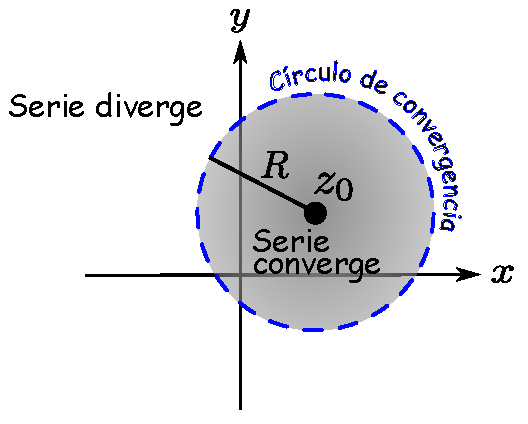
\includegraphics[scale = 0.8]{Figuras/ConvergenciaSeriePotencia.pdf}
    \caption{Región de convergencia de una serie de potencia.}
    \label{fig:CVPotencia}
\end{figure}

\subsection*{Continuidad, integración y analiticidad de las series de potencias}

Aplicando los teoremas vistos para el tratamiento de sucesiones y series de funciones, tenemos:

\begin{propo}
La suma de una serie de potencias es continua en la región de convergencia.
\end{propo}

\begin{propo}\label{IntegracionPotencia}
Si $\sum\limits_{n=0}^{\infty} a_n (z-z_0)^n$ es una serie de potencias y $\gamma$ una curva suave por trazos contenida en el interior de su círculo de convergencia, entonces
$$\int_{\gamma} \left( \sum_{n=0}^{\infty} a_n (z-z_0)^n \right) \,dz = \sum_{n=0}^{\infty} a_n \int_{\gamma} (z-z_0)^n \,dz.$$
\end{propo}

\begin{propo}\label{DerivadaPotencia}
Si $\sum\limits_{n=0}^{\infty} a_n (z-z_0)^n$ es una serie de potencias y $S(z)$ su suma, entonces $S(z)$ es derivable en cada punto $z$ al interior de su círculo de convergencia y su derivada puede obtenerse derivando término a término la serie $\sum\limits_{n=0}^{\infty} a_n (z-z_0)^n$, es decir,
$$S\,'(z) = \sum_{n=1}^{\infty} n a_n (z-z_0)^{n-1}.$$
\end{propo}

\begin{ejemplo}
Empecemos con la serie geométrica
$$\frac{1}{1 - z} = \sum_{n=0}^{\infty} z^n, \quad |z| < 1.$$

Hacemos el reemplazo $\xi = - z$ para asi obtener
$$\frac{1}{1 + \xi} = \sum_{n=0}^{\infty} (-1)^n \xi^n, \quad |\xi| < 1.$$

Como la integral de una función analítica en una bola abierta (simplemente conexo) es independiente de la curva, integramos en el segmento $[0,z]$, donde $|z| < 1$, 
$$\int_{[0,z]} \frac{1}{1+\xi} d\xi = \sum_{n=0}^{\infty} (-1)^n \int_{[0,1]} \xi^n \,d\xi.$$

Una antiderivada de la función continua $1/(1+\xi)$ en $\mathbb{C} - \{-1\}$ es $Log(1 + z)$ en la región $D = \mathbb{C}\setminus ]-\infty,-1]$. Entonces,
\begin{align*}
    Log(1+z) = \int_{[0,z]} \frac{1}{1+\xi} d\xi &= \sum_{n=0}^{\infty} \left. (-1)^n \frac{\xi^{n+1}}{n+1} \right|_{0}^z \\
    &= \sum_{n=0}^{\infty} (-1)^n \frac{z^{n+1}}{n+1}.
\end{align*}

Por lo tanto,
$$Log(1+z) = \sum_{n=0}^{\infty} (-1)^n \frac{z^{n+1}}{n+1}, \quad |z| < 1.$$
\end{ejemplo}

\begin{ejemplo}
Encuentre la suma de $\sum\limits_{n=1}^{\infty} n z^n$ y determine su radio de convergencia.
\\

\textbf{Solución:} Esta serie se ve como la derivada de la serie geométrica
$$\frac{1}{1-z} = \sum_{n=0}^{\infty} z^n, \quad |z| < 1.$$

En efecto, derivando término a término, obtenemos la serie de potencias
$$\frac{d}{dz}\left[ \frac{1}{1-z} \right] = \frac{1}{(1-z)^2} = \sum_{n=1}^{\infty} n z^{n-1}, \quad |z| < 1.$$

Multiplicando ambos lados por $z$, 
$$\frac{z}{(1-z)^2} = \sum_{n=1}^{\infty} n z^n, \quad |z| < 1.$$

En particular, el radio de convergencia es 1.
\end{ejemplo}

\begin{teorema}[Unicidad de la serie de potencias] 
Sea $R > 0$. Si para todo $z$ que satisface $|z-z_0| < R$, tenemos
$$\sum_{n=0}^{\infty} a_n (z-z_0)^n = f(z) =  \sum_{n=0}^{\infty} b_n(z-z_0)^n.$$

Entonces, $a_n = b_n$ para todo $n \in \mathbb{N}_0$. En particular, si $\sum\limits_{n=0}^{\infty} c_n (z-z_0)^n = 0$ para todo $|z-z_0| < R$, entonces $c_n = 0$ para $n = 0,1,2, \dots$
\end{teorema}

\begin{proof}
La proposición \ref{DerivadaPotencia} nos garantiza la existencia de las derivadas de orden superior para la misma región de convergencia de una serie de potencias. Entonces,
\begin{align*}
f'(z) &= \sum_{n=1}^{\infty} n a_n(z-z_0)^{n-1} = \sum_{n=1}^{\infty} n b_n(z-z_0)^{n-1} \\
f''(z) &= \sum_{n=2}^{\infty} n(n-1) a_n(z-z_0)^{n-2} = \sum_{n=2}^{\infty} n(n-1) b_n(z-z_0)^{n-2} \\
&~\vdots \\
f^{(k)} (z) &=  \sum_{n=k}^{\infty} n(n-1) \cdots (n-(k-1)) a_n(z-z_0)^{n-k} = \sum_{n=k}^{\infty} n(n-1) \cdots (n - (k-1)) b_n(z-z_0)^{n-k}.
\end{align*}

Evaluando en $z = z_0$ y considerando $f^{(0)}(z_0) = f(z_0)$:
$$\forall k \geq 0: ~ f^{(k)}(z_0) = k! a_k = k! b_k ~\Rightarrow~ a_k = b_k.$$
\end{proof}

\section{Series de Taylor}

Sea $f$ una función analítica en un dominio $D$ y sea $z_0 \in D$. Por el teorema de la fórmula integral de Cauchy, $f$ tiene derivada de todos los órdenes en $z_0$.

\begin{defi}
Se define la serie de potencias siguiente:
$$f(z_0) + \sum_{n=1}^{\infty} \frac{f^{(n)}(z_0)}{n!}(z-z_0)^n.$$

Esta serie se llama \textbf{serie de Taylor} de $f$ alrededor de $z_0$.
\end{defi}

\textbf{Observación:} Cuando $z_0 = 0$, la serie se conoce como \textbf{serie de Maclaurin} de $f$.

\begin{teorema}[de Taylor]
Sea $f$ una función analítica en un dominio $D$ y sea $z_0 \in D$. Entonces, existe $R_0 > 0$ tal que la serie de Taylor de $f$ en $z_0$
$$f(z_0) + \sum_{n=1}^{\infty} \frac{f^{(n)}(z_0)}{n!}(z-z_0)^n.$$

converge para $|z-z_0| < R_0$; más aún, su suma es $f(z)$, es decir,
$$f(z) = f(z_0) + \sum_{n=1}^{\infty} \frac{f^{(n)}(z_0)}{n!}(z-z_0)^n.$$
\end{teorema}

\begin{proof}

Dado que $D$ es abierto, elegimos el mayor $R_0 > 0$ tal que $B(z_0,R_0) \subseteq D$, es decir, el mayor disco abierto tal que $f$ sea analítica. Para $0 < R_1 < R_0$, tomamos $z$ al interior de la circunferencia $C_1: |z-z_0| = R_1$, ver figura \ref{fig:Taylor}. Como $f$ es analítica, por el teorema de la fórmula integral de Cauchy, 
$$f(z) = \frac{1}{2\pi i} \int_{C_1} \frac{f(\xi)}{\xi-z} d\xi.$$

\begin{figure}[H]
    \centering
    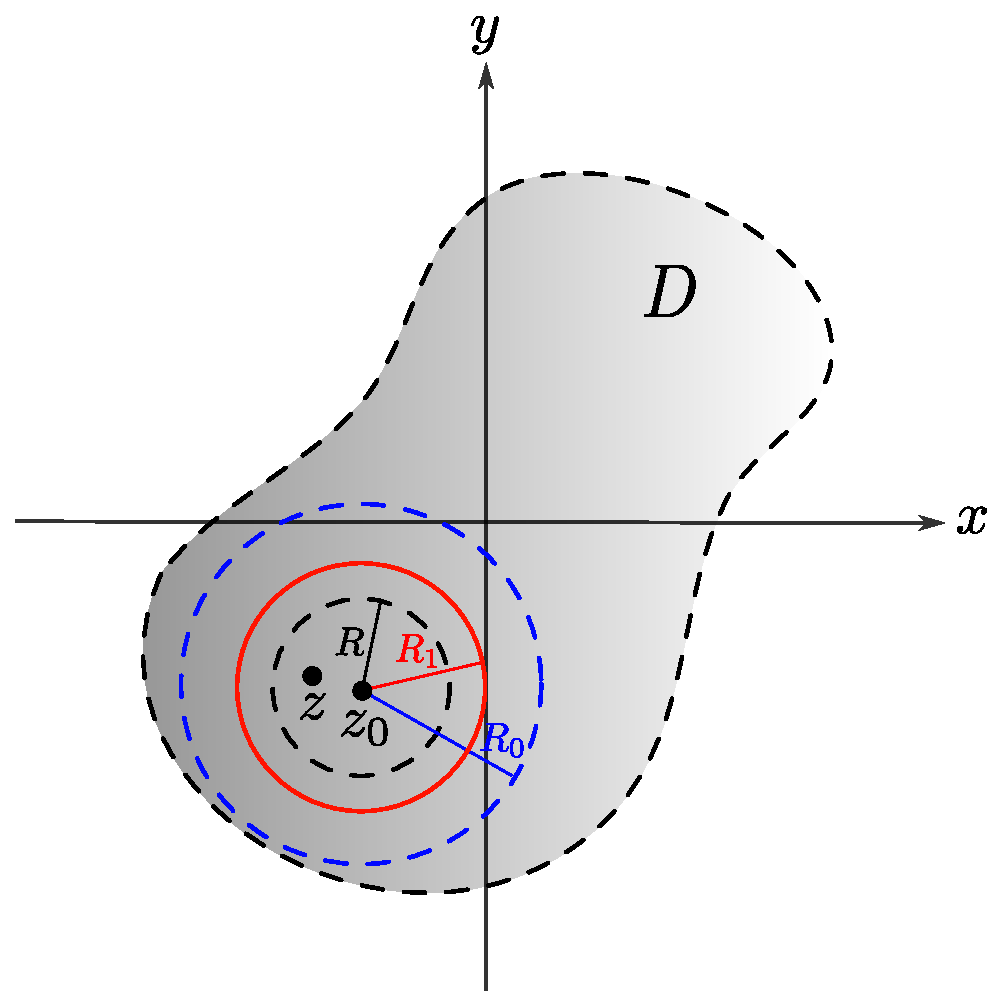
\includegraphics[scale = 0.55]{Figuras/TeoremaTaylor.pdf}
    \caption{Demostración del teorema de Taylor.}
    \label{fig:Taylor}
\end{figure}

Sea $\xi \in C_1$, notemos que
$$\frac{1}{\xi - z} = \frac{1}{(\xi - z_0) - (z-z_0)} = \frac{1}{\xi - z_0} \frac{1}{1- \frac{z-z_0}{\xi-z_0}}. $$

Del ejemplo \ref{SerieGeo}, se tiene que
$$\sum_{k=0}^n w^k = 1 + w + \cdots + w^n = \frac{1-w^{n+1}}{1-w}, \quad w \neq 1.$$

Entonces,
\begin{align*}
    \frac{1-\left(\frac{z-z_0}{\xi-z_0}\right)^N}{1- \frac{z-z_0}{\xi-z_0}} &= 1 + \frac{z-z_0}{\xi-z_0} + \left(\frac{z-z_0}{\xi-z_0} \right)^2 + \cdots + \left(\frac{z-z_0}{\xi-z_0} \right)^{N-1} \\
    \Rightarrow ~ \frac{1}{1- \frac{z-z_0}{\xi-z_0}}&=  1 + \frac{z-z_0}{\xi-z_0} + \left(\frac{z-z_0}{\xi-z_0} \right)^2 + \cdots + \left(\frac{z-z_0}{\xi-z_0} \right)^{N-1} + \frac{1}{1-\frac{z-z_0}{\xi-z_0}} \left(\frac{z-z_0}{\xi-z_0} \right)^{N}.
\end{align*}

Así,
\begin{align*}
    \frac{1}{\xi-z} &= \frac{1}{\xi-z_0}  \frac{1}{1- \frac{z-z_0}{\xi-z_0}} \\
    &= \frac{1}{\xi-z_0} \left(  1 + \frac{z-z_0}{\xi-z_0} + \left(\frac{z-z_0}{\xi-z_0} \right)^2 + \cdots + \left(\frac{z-z_0}{\xi-z_0} \right)^{N-1} + \frac{1}{1-\frac{z-z_0}{\xi-z_0}} \left(\frac{z-z_0}{\xi-z_0} \right)^{N}\right) \\
    &= \frac{1}{\xi-z_0} + \frac{z-z_0}{(\xi-z_0)^2} + \cdots + \frac{(z-z_0)^{N-1}}{(\xi - z_0)^N} + \frac{(z-z_0)^N}{(\xi-z)(\xi - z_0)^N}.
\end{align*}

Luego,
\begin{align*}
    \frac{f(\xi)}{\xi-z} &= \frac{f(\xi)}{\xi-z_0} +(z-z_0) \frac{f(\xi)}{(\xi-z_0)^2} + (z-z_0)^2 \frac{f(\xi)}{(\xi-z_0)^3} + \cdots \\ & ~ + (z-z_0)^{N-1}\frac{f(\xi)}{(\xi - z_0)^N} +(z-z_0)^N \frac{f(\xi)}{(\xi-z)(\xi - z_0)^N}.
\end{align*}

Ahora, integrando ambos lados por $\frac{1}{2\pi i} \int_{C_1}$, tenemos
\begin{align*}
    f(z) &= \frac{1}{2\pi i} \int_{C_1} \frac{f(\xi)}{\xi-z} \,d\xi \\
    &= \frac{1}{2\pi i} \int_{C_1} \frac{f(\xi)}{\xi-z_0} \,d\xi + (z-z_0) \frac{1}{2\pi i} \int_{C_1} \frac{f(\xi)}{(\xi-z)^2} \,d\xi + (z-z_0)^2 \frac{1}{2\pi i} \int_{C_1} \frac{f(\xi)}{(\xi-z_0)^3} \,d\xi + \cdots \\
    &~+ (z-z_0)^{N-1} \frac{1}{2\pi i} \int_{C_1} \frac{f(\xi)}{(\xi-z_0)^N} \,d\xi + (z-z_0)^N \frac{1}{2\pi i} \int_{C_1} \frac{f(\xi)}{(\xi - z)(\xi - z_0)^N} \,d\xi \\
    &= f(z_0) + f'(z_0) (z-z_0) + \frac{f''(z_0)}{2!}(z-z_0)^2 + \frac{f^{(3)}(z_0)}{3!} (z-z_0)^3 + \cdots \\
    & ~+ \frac{f^{(N-1)}(z_0)}{(N-1)!} (z-z_0)^{N-1} + R_N(z), 
\end{align*}

donde 
$$R_N(z) =  \frac{(z-z_0)^N}{2\pi i} \int_{C_1} \frac{f(\xi)}{(\xi - z)(\xi - z_0)^N} \,d\xi.$$

Recordemos que $ |z-z_0| < R < R_1$ y $|\xi-z_0| = R_1$, de donde se obtiene
$$|\xi-z| \geq ||\xi - z_0| - |z-z_0|| \geq |\xi-z_0| - |z-z_0| > R_1 - R.$$

Luego, si $|f(\xi)| \leq M$ para $\xi \in C_1$ (compacto), entonces
$$|R_N(z)| \leq \frac{R^N}{2\pi} \frac{2\pi R_1 M}{(R_1 - R)R_1^N} = \frac{MR_1}{R_1- R} \left( \frac{R}{R_1}\right)^{N}.$$

Como $0 < \frac{R}{R_1} < 1$, se tiene que
$$\lim_{N \to + \infty} R_N(z) = 0,$$

probando así el teorema.
\end{proof}

\begin{ejemplo}
Encuentre las series de Maclaurin de 
$$(a) ~e^z, \quad (b)~ \cos z, \quad (c) ~\sin z. $$

\textbf{Solución:} Notemos que las tres funciones son enteras, así que las series de Maclaurin convergerán para todo $z \in \mathbb{C}$.

\begin{itemize}
    \item[(a)] Si $f(z) = e^z$, entonces
    $$\forall n \in \mathbb{N}: ~ f^{(n)}(z) = e^z \Rightarrow f^{(n)}(0) = 1.$$
    
    Por lo tanto, la serie de Macluarin es
    $$e^z = \sum_{n=0}^{\infty} \frac{f^{(n)}(0)}{n!} z^n = \sum_{n=0}^{\infty} \frac{z^n}{n!}, \quad \forall z \in \mathbb{C}.$$
    
    \item[(b)] Notemos que 
    \begin{align*}
f(z) = \cos(z) &\Rightarrow f(0) = 1; \\
f'(z) = -\sin(z)&\Rightarrow  f'(0) = 0; \\
f''(z) = - \cos(z)  &\Rightarrow  f''(0) = -1; \\
f^{(3)} (z) = \sin(z) &\Rightarrow f^{(3)}(0) = 0; \\
f^{(4)}(z) = \cos(z)  &\Rightarrow  f^{(4)}(0) = 1 \\
&\vdots
\end{align*}

Es decir,
$$\forall n \geq 0:~ f^{(2n)}(0) = (-1)^n ~~\mbox{y}~~ f^{(2n+1)}(0) = 0.$$

Por lo tanto, la serie de Maclaurin  es
$$\cos(z) = \sum_{n=0}^{\infty} \frac{(-1)^n}{(2n)!} z^{2n}.$$

    \item[(C)] Usando la relación $\frac{d}{dz} \cos(z) = - \sin(z)$ y la serie para el coseno,
    \begin{align*}
        \sin(z) = - \frac{d}{dz} \cos(z) = - \frac{d}{dz}\left[\sum_{n=0}^{\infty} \frac{(-1)^n}{(2n)!} z^{2n} \right] &= - \sum_{n=1}^{\infty} \frac{(-1)^n 2n}{(2n)!} z^{2n-1} \\
        &= \sum_{n=1}^{\infty} \frac{(-1)^{n+1}}{(2n-1)!} z^{2n-1} \\
        &= \sum_{n=0}^{\infty} \frac{(-1)^{n}}{(2n+1)!} z^{2n+1}.
    \end{align*}
\end{itemize}
\end{ejemplo}

\begin{ejemplo}
Encontrar la serie de Taylor de 
$$\frac{1}{4-iz}$$

alrededor del $z_0 = 3$ y determine su radio de convergencia.
\\

\textbf{Solución:} La función es analítica en $\mathbb{C} \setminus \{-4i\}$. Su serie de Taylor alrededor de $z_0 = 3$ converge en la bola abierta centrada en $3$ con radio hasta llegar a la singularidad $-4i$. Como $|3-4i| = 5$, concluimos que el radio de convergencia de la serie debería ser $5$. Para encontrar la serie de Taylor desarrollemos  $\frac{1}{4-iz}$ de tal forma que su denominador aparezca una expresión tipo $1-w$ con $w = a(z-z_0) = a(z-3)$ donde $a \in \mathbb{C}$:

\begin{align*}
    \frac{1}{4-iz} = \frac{1}{i(-4i-z)} = \frac{-i}{-4i -z} 
    &= \frac{-i}{-4i-3-(z-3)} \\
    &= \frac{-i}{-3-4i} \frac{1}{1 - \frac{z-3}{-3-4i}} \\
    &=  \frac{-i}{-3-4i} \frac{1}{1 - w} \\
    &= \frac{-i}{-3-4i} \sum_{n=0}^{\infty} w^n \\
    &= \frac{-i}{-3-4i} \sum_{n=0}^{\infty} \left(\frac{z-3}{-3-4i} \right)^n \\
    &= -i \sum_{n=0}^{\infty} \frac{(z-3)^n}{(-3-4i)^{n+1}}.
\end{align*}

Esta serie converge si y sólo si $|w| < 1$, equivalentemente,
$$\left|\frac{z-3}{-3-4i} \right| < 1 \Leftrightarrow |z-3| < |-3-4i| = 5,$$

lo cual confirma que el radio de convergencia de la serie es 5.
\end{ejemplo}

\subsection*{Multiplicación de series de potencias*}

\begin{teorema}[Multiplicación de series de potencias]
Dados dos desarrollos en serie de potencias en torno del origen, por ejemplo
$$f(z) = \sum_{n=0}^{\infty} a_n z^n, \quad |z| < R$$

y
$$g(z) = \sum_{n=0}^{\infty} b_n z^n, \quad |z| < R.$$

El producto $f(z) g(z)$ viene dado por la serie de potencias
$$f(z) g(z) = \sum_{n=0}^{\infty} c_n z^n, \quad |z| < R$$

en donde 
$$c_n = \sum_{k=0}^n a_k b_{n-k}; \quad n = 0,1,2, \dots$$
\end{teorema}

\begin{proof}
Sea $D = \{z \in \mathbb{C} : |z| < R\}$. Entonces, $f$ y $g$ son analíticas en $D$, luego $f \cdot g$ es también analítica en $D$. 

Por el teorema de Taylor,
$$(f\cdot g)(z) = \sum_{n=0}^{\infty} \frac{(f\cdot g)^{(n)}(0)}{n!} z^n, \quad z \in D.$$

Probaremos por inducción que
\begin{equation}
 (f\cdot g)^{(n)}(z) = \sum_{k=0}^n \binom{n}{k} f^{(k)}(z) g^{(n-k)}(z).   \label{DerivadaProductNesima}
\end{equation}

Para $n = 0$:
$$(f \cdot g)(z) = \binom{0}{0} f^{(0)}(z) g^{(0)}(z).$$

Supongamos que para todo $n \in \mathbb{N}_0$ se verifica \eqref{DerivadaProductNesima}. Buscamos probar que 
$$(f\cdot g)^{(n+1)}(z) = \sum_{k=0}^{n+1} \binom{n+1}{k} f^{(k)}(z) g^{(n+1-k)}(z).$$

Para ello, calculemos:
\begin{align*}
   (f\cdot g)^{(n+1)}(z) &= \frac{d}{dz} \left[ (f\cdot g)^{(n)}(z) \right]  \\
   &= \sum_{k=0}^n \binom{n}{k} \left[ f^{(k+1)}(z) g^{(n-k)}(z) + f^{(k)}(z) g^{(n+1-k)}(z) \right] \\
   &= \sum_{k=0}^n \binom{n}{k} f^{(k)}(z) g^{(n+1-k)}(z) + \sum_{k=0}^n \binom{n}{k} f^{(k+1)}(z) g^{(n-k)}(z) \\
   &= \binom{n}{0} f(z) g^{(n+1)}(z) +  \sum_{k=1}^n \binom{n}{k} f^{(k)}(z) g^{(n+1-k)}(z) \\
   &~+ \sum_{k=0}^{n-1} \binom{n}{k} f^{(k+1)}(z) g^{(n-k)}(z) + \binom{n}{n} f^{(n+1)}(z) g(z) \\
   &= \binom{n}{0} f(z) g^{(n+1)}(z) +  \sum_{k=1}^n \binom{n}{k} f^{(k)}(z) g^{(n+1-k)}(z) \\
   &~+ \sum_{k=1}^{n} \binom{n}{k-1} f^{(k)}(z) g^{(n+1-k)}(z) + \binom{n}{n} f^{(n+1)}(z) g(z) 
\end{align*}
\begin{align*}
   &= \binom{n+1}{0} f(z) g^{(n+1)}(z) +  \sum_{k=1}^n \left[\binom{n}{k-1} +  \binom{n}{k} \right] f^{(k)}(z) g^{(n+1-k)}(z) \\
   &~+ \binom{n+1}{n+1} f^{(n+1)}(z) g(z) \\
   &= \binom{n+1}{0} f(z) g^{(n+1)}(z) +  \sum_{k=1}^n \binom{n+1}{k} f^{(k)}(z) g^{(n+1-k)}(z) + \binom{n+1}{n+1} f^{(n+1)}(z) g(z) \\
   &= \sum_{k=0}^{n+1} \binom{n+1}{k} f^{(k)}(z) g^{(n+1-k)}(z).
\end{align*}

Luego,
$$ \frac{(f\cdot g)^{(n)}(0)}{n!} = \sum_{k=0}^n \frac{f^{(k)}(0) g^{(n-k)}(0)}{(n-k)!k!}   = \sum_{k=0}^n \frac{a_k k! b_{n-k} (n-k)!}{(n-k)!k!}   = \sum_{k=0}^n a_k b_{n-k}.$$

Así, la serie $\sum\limits_{n=0}^{\infty} c_n z^n$ converge en $D$ y
$$(f\cdot g)(z) = \sum_{k=0}^{\infty} c_n z^n = \left(\sum_{k=0}^{\infty} a_n z^n \right) \cdot \left(\sum_{k=0}^{\infty} b_n z^n \right).$$
\end{proof}

En otras palabras, se entiende el producto de series de potencias como el producto de polinomios aprendido en los cursos básicos de matemática, es decir,
\begin{align*}
\left(\sum_{n=0}^{\infty} a_n z^n \right) \cdot \left(\sum_{n=0}^{\infty} b_n z^n \right) &= (a_0 + a_1 z + a_2 z^2 + \cdots ) \cdot (b_0 + b_1 z + b_2z^2 + \cdots) \\
&= a_0 b_0 + (a_0 b_1 + a_1 b_0) z + (a_0 b_2 + a_1 b_1 + a_2 b_0) z^2 + \cdots 
\end{align*} 

\section{Series de Laurent}

Vimos en la sección anterior que si una función es analítica en un disco abierto centrado en $z_0$, entonces admite una representación en serie de Taylor en el disco. Existe una representación en serie similar que contiene los términos con exponentes positivos y negativos de $(z-z_0)$ para funciones que son analíticas en una región anular alrededor del punto $z_0$. Estas series son conocidas como \textbf{series de Laurent}. 

Para $0 \leq R_1 < R_2 \leq \infty$, definimos la región anular como el anillo
$$A_{R_1,R_2}(z_0) = \{z \in \mathbb{C} : R_1 < |z-z_0| < R_2\}.$$

\begin{figure}[H]
    \centering
    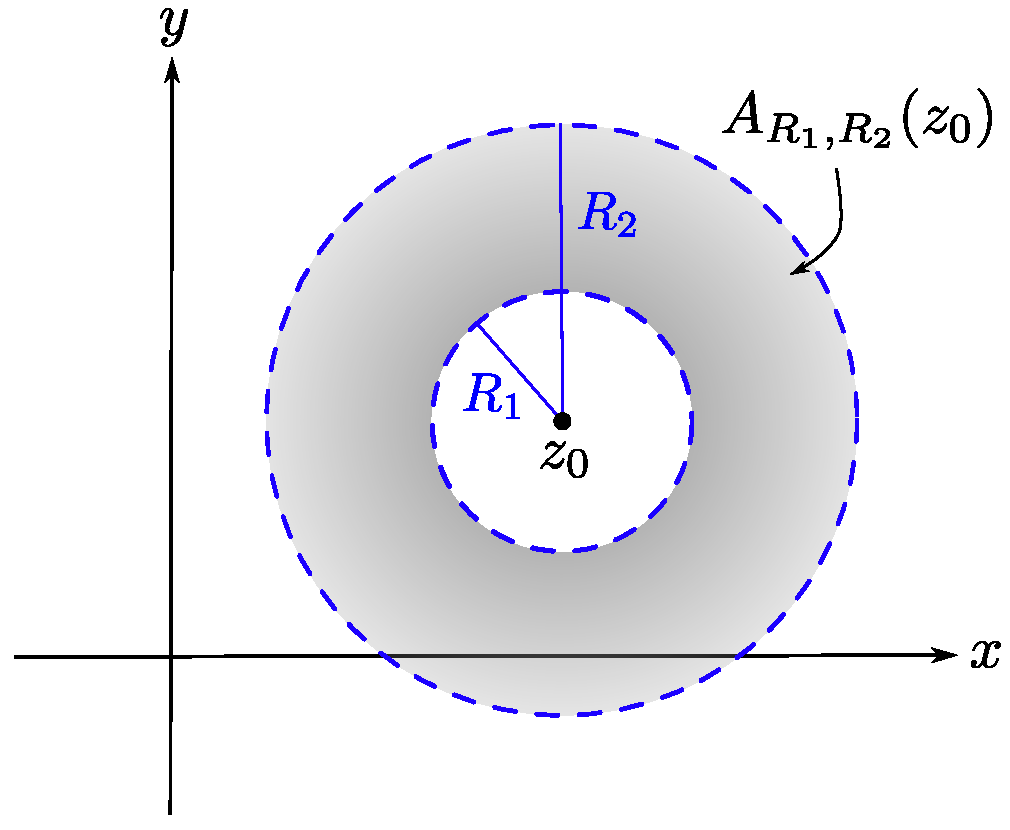
\includegraphics[scale = 0.45]{Figuras/RegionAnular.pdf}
    \caption{Región anular $A_{R_1,R_2}(z_0)$.}
    \label{fig:Annulus}
\end{figure}

\textbf{Observación:} La región anular $A_{R_1,R_2}(z_0)$ se degenera en un disco abierto sin su centro cuando $R_1 = 0$ y $R_2 < \infty$, en un plano sin el centro $z_0$ cuando $R_1 = 0$ y $R_2 = + \infty$, o un plano con un disco centrado en $z_0$ removido cuando $R_1 > 0$ y $R_2 = \infty$.

\begin{teorema}
Si $f$ es analítica en la región anular $A_{R_1,R_2}(z_0)$ donde $0 \leq R_1 < R_2 \leq \infty$. Entonces $f$ tiene una única representación como serie de la forma
\begin{equation}
f(z) = \sum_{n=0}^{\infty} a_n (z-z_0)^n + \sum_{n=1}^{\infty} \frac{b_n}{(z-z_0)^n}, \quad R_1 < |z-z_0| < R_2    \label{SerieLaurent}
\end{equation}

la cual converge absolutamente para $z \in A_{R_1,R_2}(z_0)$ y uniformemente en cada región anular cerrada $\rho_1 \leq |z-z_0| \leq \rho_2$ donde $R_1 < \rho_1$ y $\rho_2 < R_2$. La serie \eqref{SerieLaurent} es llamada \textbf{serie de Laurent} de $f$ y los coeficientes $a_n$ y $b_n$ están dados por:
\begin{align}
    a_n &= \frac{1}{2\pi i} \int_{C_{R}(z_0)} \frac{f(\xi)}{(\xi-z_0)^{n+1}} \,d \xi, \quad n = 0,1,2, \dots \label{CoeLauranet1} \\
    b_n &= \frac{1}{2\pi i} \int_{C_{R}(z_0)} \frac{f(\xi)}{(\xi-z_0)^{-n+1}} \,d \xi, \quad n = 1,2,3, \dots \label{CoeLauranet2}
\end{align}

con $C_{R}(z_0)$ una circunferencia centrada en $z_0$ con radio $R_1 < R < R_2$ orientada positivamente.
\end{teorema}

\begin{proof}

Probaremos que la serie \eqref{SerieLaurent} converge absolutamente y uniformemente en la región anular cerrada $\rho_1 \leq |z-z_0| \leq \rho_2$, donde $R_1 < \rho_1$ y $R_2 < \rho_2$. Fijando $\rho_1$ y $\rho_2$, escogemos $r_1$ y $r_2$ tales que
$$R_1 < r_1 < \rho_1 < \rho_2 < r_2 < R_2$$

y encontramos un $\rho$ tal que $C_{\rho}(z)$ esté contenida en $A_{r_1, r_2}(z_0)$, lo cual es posible porque la región es abierta (ver figura \ref{fig:TeoLaurent}).

\begin{figure}[H]
    \centering
    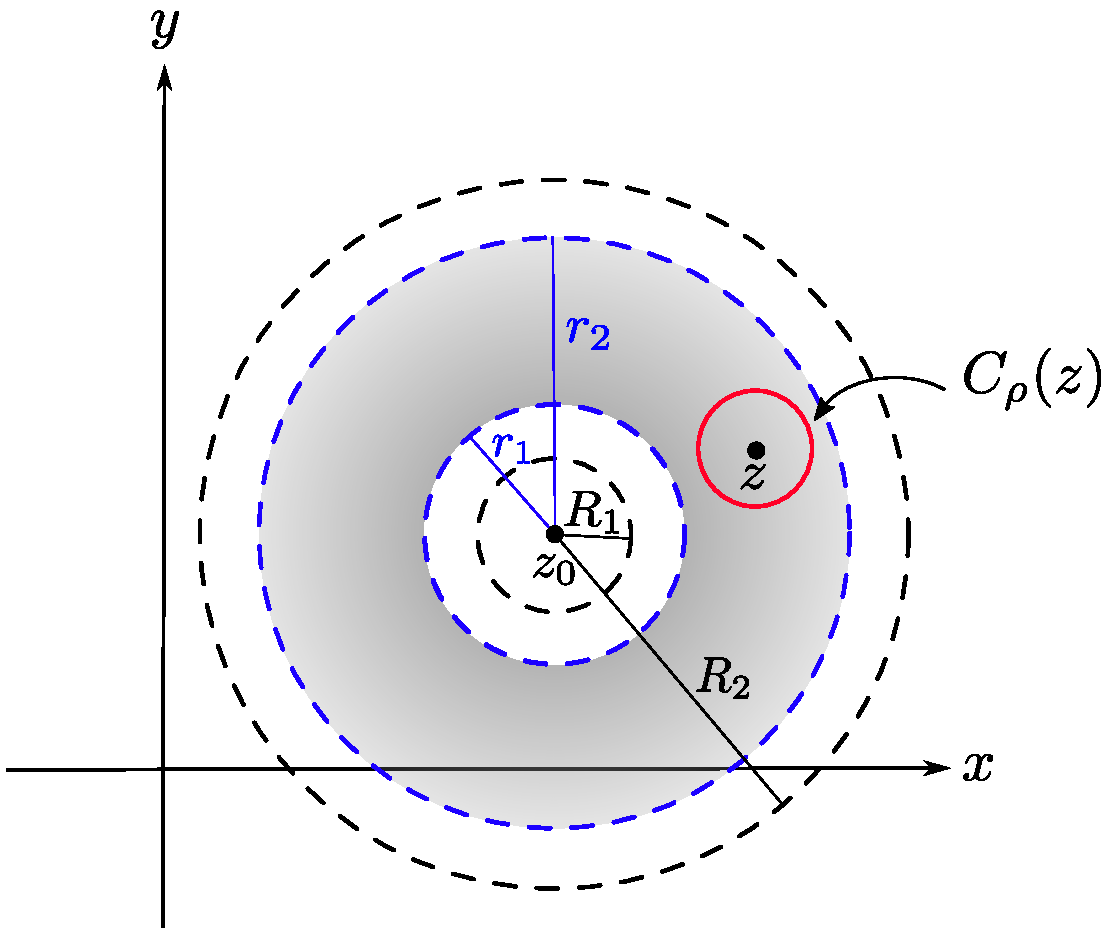
\includegraphics[scale = 0.5]{Figuras/TeoremaLaurent.pdf}
    \caption{Demostración teorema de Laurent.}
    \label{fig:TeoLaurent}
\end{figure}

La función
$$g(\xi) = \frac{f(\xi)}{\xi - z}$$

es analítica en el interior y en la frontera de la región fuera de $C_{\rho}(z)$ y al interior de $A_{r_1,r_2}(z_0)$. Entonces, por el teorema de Cauchy para regiones múltiplemente conexas, tenemos 
$$\frac{1}{2\pi i} \int_{C_{r_2}(z_0)} \frac{f(\xi)}{\xi -z} \,d\xi = \frac{1}{2\pi i} \int_{C_{\rho}(z)} \frac{f(\xi)}{\xi-z} d\xi + \frac{1}{2\pi i} \int_{C_{r_1}(z_0)} \frac{f(\xi)}{\xi - z} \,d\xi,$$

donde todas las circunferencias están orientadas positivamente. Por la fórmula integral de Cauchy, la primera integral al lado derecho de la igualdad es $f(z)$, porque $f$ es analítica dentro de la región anular $A_{R_1,R_2}(z_0)$, más aún al interior de una pequeña vecindad que contiene a $C_{\rho}(z)$. Así,
\begin{equation}
 f(z) = \frac{1}{2\pi i} \int_{C_{r_2}(z_0)} \frac{f(\xi)}{\xi - z} \,d\xi - \frac{1}{2\pi i}  \int_{C_{r_1}(z_0)} \frac{f(\xi)}{\xi - z} \,d\xi. \label{DemLaurent1}
\end{equation}

Para $\xi \in C_{r_2}(z_0)$ y $z$ satisfaciendo $\rho_1 \leq |z-z_0| \leq \rho_2$, tenemos 
$$\frac{|z-z_0|}{|\xi-z_0|} \leq \frac{\rho_2}{r_2} < 1.$$

Luego, podemos escribir
$$\frac{1}{\xi-z} = \frac{1}{\xi - z_0 - (z-z_0)} = \frac{\frac{1}{\xi-z_0}}{1 - \frac{z-z_0}{\xi-z_0}} = \sum_{n=0}^{\infty} \frac{(z-z_0)^n}{(\xi-z_0)^{n+1}}$$

y la serie converge absolutamente y uniformemente en $\xi$ tal que $|\xi-z_0| = r_2$. Entonces, multiplicando por $\frac{1}{2\pi i} f(\xi)$ ambos lados e integrando sobre la circunferencia $C_{r_2}(z_0)$, obtenemos
$$\frac{1}{2\pi i} \int_{C_{r_2}(z_0)} \frac{f(\xi)}{\xi - z} \,d\xi = \sum_{n=0}^{\infty} a_n (z-z_0)^n,$$

donde
\begin{equation}
a_n = \frac{1}{2\pi i} \int_{C_{r_2}(z_0)} \frac{f(\xi)}{(\xi-z_0)^{n+1}} \,d\xi, \quad n = 0,1,2, \dots    \label{DemLaurent2}
\end{equation}

Para la segunda integral al lado derecho de \eqref{DemLaurent1}, tenemos que para $ \xi \in C_{r_1}(z_0)$ y $z$ tales que $\rho_1 \leq |z-z_0| \leq \rho_2$,
$$\frac{|\xi-z_0|}{|z-z_0|} \leq \frac{r_1}{\rho_1} < 1.$$

Luego, podemos escribir
$$\frac{1}{\xi-z} = \frac{1}{\xi - z_0 - (z-z_0)} = \frac{-\frac{1}{z-z_0}}{1 - \frac{\xi-z_0}{z-z_0}} = \sum_{n=0}^{\infty} \frac{-(\xi-z_0)^n}{(z-z_0)^{n+1}} = - \sum_{n=1}^{\infty} \frac{(\xi-z_0)^{n-1}}{(z-z_0)^n}$$

y la serie converge absolutamente y uniformemente en $\xi$ tal que $|\xi-z_0| = r_1$. Entonces, multiplicando por $-\frac{1}{2\pi i} f(\xi)$ ambos lados e integrando sobre la circunferencia $C_{r_1}(z_0)$, obtenemos
\begin{align*}
 -\frac{1}{2\pi i} \int_{C_{r_1}(z_0)} \frac{f(\xi)}{\xi - z} \,d\xi &= \sum_{n=1}^{\infty} \left\{ \frac{1}{2\pi i} \int_{C_{r_1}(z_0)} f(\xi) (\xi - z_0)^{n-1} \,d\xi\right\} \frac{1}{(z-z_0)^n} \\
 &= \sum_{n=1}^{\infty} \frac{b_n}{(z-z_0)^n},
\end{align*}

donde 
\begin{equation}
b_n =  \frac{1}{2\pi i} \int_{C_{r_1}(z_0)} \frac{f(\xi)}{(\xi - z_0)^{-n+1}} \,d\xi, \quad n = 1,2, \dots   \label{DemLaurent3}
\end{equation}

Ahora, para $R \in \,]R_1, R_2[$, por el teorema de deformación, las expresiones \eqref{DemLaurent2} y \eqref{DemLaurent3} son equivalentes a \eqref{CoeLauranet1} y \eqref{CoeLauranet2}, respectivamente.

Finalmente, demostremos la unicidad de la expansión en serie de Laurent. Supongamos que en la región anular $A_{R_1,R_2}(z_0)$ la función $f$ tiene dos series de Laurent:
$$ f(z) = \sum_{n=0}^{\infty} a_n (z-z_0)^n + \sum_{n=1}^{\infty} \frac{b_n}{(z-z_0)^n} = \sum_{n=0}^{\infty} c_n (z-z_0)^n + \sum_{n=1}^{\infty} \frac{d_n}{(z-z_0)^n},$$

las cuales convergen uniformemente en toda subregión anular cerrada de $A_{R_1,R_2}(z_0)$. Multiplicando por $\frac{1}{2\pi i}(z-z_0)^{-k-1}$ ambos lados, con $k \in \mathbb{Z}$, obtenemos que 
\begin{align*}
& \frac{1}{2\pi i}\sum_{n=0}^{\infty} a_n (z-z_0)^{n-k-1} + \frac{1}{2\pi i} \sum_{n=1}^{\infty} b_n (z-z_0)^{-n-k-1} \\
&= \frac{1}{2\pi i} \sum_{n=0}^{\infty} c_n (z-z_0)^{n-k-1} + \frac{1}{2\pi i} \sum_{n=1}^{\infty} d_n (z-z_0)^{-n-k-1}.    
\end{align*}

Ahora, gracias a la convergencia uniforme, integramos término a término las series sobre la circunferencia $C_R(z_0)$ con $R_1 < R < R_2$.
\begin{align*}
&\sum_{n=0}^{\infty}  \frac{1}{2\pi i} \int_{C_R(z_0)}a_n (z-z_0)^{n-k-1} \,dz +  \sum_{n=1}^{\infty} \frac{1}{2\pi i}   \int_{C_R(z_0)} b_n (z-z_0)^{-n-k-1} \,dz \\
&=  \sum_{n=0}^{\infty} \frac{1}{2\pi i} \int_{C_R(z_0)}  c_n (z-z_0)^{n-k-1} \,dz  +  \sum_{n=1}^{\infty} \frac{1}{2\pi i} \int_{C_R(z_0)}  d_n (z-z_0)^{-n-k-1} \,dz.    
\end{align*}

Como
$$\int_{C_R(z_0)} (z-z_0)^m \,dz = \left\{ \begin{array}{cl}
    0, &  \mbox{si} ~ m \neq -1\\
     2\pi i ,& \mbox{si} ~ m = -1
\end{array} \right. ,$$

concluimos que para $k \geq 0$, la integral de cada término de las segundas series y todos los de las primeras, excepto aquel para el que $n = k$, es 0. Por lo tanto,
$$a_k = c_k, \quad k = 0,1,2,\dots$$

y para $k \leq -1$, la integral de todos los términos es 0, excepto aquel de las segundas series con $n = -k$. Por lo tanto,
$$b_{-k} = d_{-k} \Rightarrow b_k = d_k, \quad k = 1,2, \dots$$
\end{proof}

\textbf{Observación:} Si llamamos a $b_n = a_{-n}$, entonces podemos denotar la serie de Laurent por
$$f(z) = \sum_{n= - \infty}^{\infty} a_n (z-z_0)^n$$

con
$$a_n = \frac{1}{2\pi i} \int_{C_R(z_0)} \frac{f(\xi)}{(\xi - z_0)^{n+1}}, \quad n = 0,\pm 1, \pm 2, \dots$$

\begin{ejemplo}
Determinar la serie de Laurent de la función
$$f(z) = \frac{z+1}{z}$$

dentro de la región anular $|z| > 0$.
\\

\textbf{Solución:} Es claro que $f$ es analítica en $\{z \in \mathbb{C}: |z| > 0\} = \mathbb{C} \setminus\{0\}$, luego $f$ admite una representación en serie de Laurent en $\mathbb{C} \setminus\{0\}$. Sea $\gamma$ la circunferencia $|z| = R > 0$, calculemos los coeficientes de la serie:
$$a_n = \frac{1}{2\pi i} \int_{\gamma} \frac{\frac{\xi +1}{\xi}}{\xi^{n+1}} \,d\xi = \frac{1}{2\pi i} \int_{\gamma} \frac{\xi +1}{\xi^{n+2}} \,d\xi = \left\{ \begin{array}{cl}
        1, & \mbox{si}~ n = 0  \\
        0, & \mbox{si}~ n = 1,2, \dots
    \end{array} \right. .$$

y
$$ b_n = \frac{1}{2\pi i} \int_{\gamma} \frac{\frac{\xi +1}{\xi}}{\xi^{-n+1}} \,d\xi = \frac{1}{2\pi i} \int_{\gamma} \frac{\xi +1}{\xi^{-n+2}} \,d\xi = \left\{ \begin{array}{cl}
        1, & \mbox{si}~ n = 1  \\
        0, & \mbox{si} ~n = 2,3, \dots
    \end{array} \right. .
$$

Por lo tanto, la serie de Laurent es
$$\frac{z+1}{z} = 1 + \frac{1}{z}.$$

Sin embargo, note que se obtiene el mismo resultado al simplemente separar la función en dos fracciones, lo cual hace ridículo el cálculo anterior hecho. En general, se recomienda no calcular los coeficientes por medio de las integrales, pues puede resultar bastante laborioso y no trivial. Por esta razón, se sugiere recurrir a series ya conocidas de otras funciones y tener siempre presente la unicidad de las series de Laurent.
\end{ejemplo}

\begin{ejemplo}
Determinar la serie de Laurent de
$$f(z) = \frac{z}{z^2+1}$$

en la región anular $0 < |z-i| < 2$ ($z_0 = i$).
\\

\textbf{Solución:}  Es claro que $f$ es analítica en $A = \{z \in \mathbb{C}: 0< |z-i| < 2\}$, luego $f$ admite una representación en serie de Laurent en $A$. Encontremos esta serie, para ello notemos que
\begin{align}
    \frac{z}{z^2+1} = \frac{z}{(z+i)(z-i)} = \left( \frac{z}{z+i}\right) \frac{1}{z-i} &= \left( \frac{z+i-i}{z+i}\right) \frac{1}{z-i} \nonumber\\
    &=\left(1 - i\frac{1}{z+i}\right) \frac{1}{z-i} \label{EjLaurent1}
\end{align}

Encontremos una expansión en serie de $\frac{1}{z+i}$, con este fin, trabejemos un poco la expresión.
\begin{align*}
    \frac{1}{z+i} = \frac{1}{2i + (z-i)} = \frac{1}{2i} \left( \frac{1}{1+\frac{z-i}{2i}} \right) &= \frac{1}{2i} \left( \frac{1}{1-\left(-\frac{z-i}{2i}\right)} \right) \\
    &= \frac{1}{2i} \sum_{n=0}^{\infty} \left(-\frac{z-i}{2i} \right)^n \\
    &=  \frac{1}{2i} \sum_{n=0}^{\infty} (-1)^n \left(\frac{z-i}{2i} \right)^n \\
    &= \sum_{n=0}^{\infty} (-1)^n \frac{(z-i)^n}{(2i)^{n+1}},
\end{align*}

la cual converge si y sólo si
$$\left| - \frac{z-i}{2i} \right| < 1 \Leftrightarrow |z-i| < 2.$$

Reemplazando en \eqref{EjLaurent1}, tenemos
\begin{align*}
 \frac{z}{z^2+1} = \left( 1 - i \sum_{n=0}^{\infty} (-1)^n \frac{(z-i)^n}{(2i)^{n+1}} \right) \frac{1}{z-i} &= \frac{1}{z-i} - i \sum_{n=0}^{\infty} (-1)^n \frac{(z-i)^{n-1}}{(2i)^{n+1}} \\
 &=  \frac{1}{z-i} - \frac{i}{2i(z-i)} - i\sum_{n=1}^{\infty} (-1)^n \frac{(z-i)^{n-1}}{(2i)^{n+1}} \\
 &= \frac{1}{2(z-i)} - i\sum_{n=0}^{\infty} (-1)^{n+1} \frac{(z-i)^n}{(2i)^{n} (2i)^2} \\
 &=  \frac{1}{2(z-i)} - \frac{i}{4}\sum_{n=0}^{\infty} (-1)^{n} \frac{(z-i)^n}{(2i)^{n}} .
\end{align*}

Notar que de aquí podemos concluir que los coeficientes de la serie de Laurent son:
$$b_n = 0, ~ n > 1; ~ b_1 = \frac{1}{2}; ~ a_n = - \frac{i}{4} \left( -\frac{1}{2i}\right)^n, n\geq 0.$$
\end{ejemplo}

Sabemos que la serie de Laurent converge uniformemente, por lo tanto para $R_1 < |z-z_0| < R_2$, podemos derivar la serie \eqref{SerieLaurent},
$$f'(z) = \sum_{n=1}^{\infty} n a_n (z-z_0)^{n-1} - \sum_{n=1}^{\infty} \frac{n b_n}{(z-z_0)^{n+1}},$$

y la podemos integrar sobre cualquier curva $\gamma$ contenida en $A_{R_1,R_2}(z_0)$,
$$\int_{\gamma} f(z) \,dz = \sum_{n=0}^{\infty} a_n \int_{\gamma} (z-z_0)^n dz + \sum_{n=1}^{\infty} b_n \int_{\gamma} \frac{1}{(z-z_0)^n} \,dz.$$
\chapter{Residuos y polos}

\section{Singularidades y residuos}

Recordemos que un punto $z_0$ es una \textit{punto singular} de $f$, si ésta no es analítica en $z_0$ pero es analítica en algún punto de cada vecindad de $z_0$. Por ejemplo, tenemos que 0 es un punto singular de $1/z$ y, también, de $Log(z)$. De hecho, en esta última función, cada punto del semieje real negativo es un punto singular de $Log(z)$.

\begin{defi}
Un punto $z_0$ se dice \textbf{singular aislado} de $f$ si existe una vecindad de $z_0$ donde $f$ es analítica excepto en $z_0$.
\end{defi}

\begin{ejemplo}
El 0 es un punto aislado de $1/z$, pero no es punto aislado de $Log(z)$, pues toda vecindad centrada en el origen contiene puntos del semieje real negativo, en los que $Log(z)$ no es analítica.
\end{ejemplo}

\begin{ejemplo}
La función
$$\frac{z+1}{z^3(z^2+1)}$$

tiene tres puntos singulares aislados: $z = 0, \pm i$.
\end{ejemplo}

\begin{ejemplo}
La función 
$$\frac{1}{\sin(\pi z)}$$

tiene como puntos singulares aislados los $z = n \in \mathbb{Z}$.

En cambio, la función
$$\frac{1}{\sin\left( \frac{\pi}{z} \right)}$$

tiene los puntos singulares $z = 0$ y $z = 1/n$, con $n = \pm 1, \pm 2, \dots$, situados todos en el segmento del eje real entre $z = -1$ y $z = 1$. Cada punto singular, salvo $z = 0$, es aislado. El punto singular $z = 0$ no es aislado porque para toda vecindad centrada en el origen, existe $N \in \mathbb{N}$ tal que para $n \geq N$, $\frac{1}{n}$ pertenece a la vecindad.
\end{ejemplo}

Si $f$ admite un punto singular aislado en $z_0$, entonces existe $R > 0$ tal que $f$ es analítica en $0 < |z-z_0| < R$ y, por Laurent,
$$f(z) = \sum_{n=0}^{\infty} a_n (z-z_0)^n + \sum_{n=1}^{\infty} \frac{b_n}{(z-z_0)^n},$$

donde
\begin{align*}
    a_n &= \frac{1}{2\pi i} \int_C \frac{f(\xi)}{(\xi-z_0)^{n+1}} \,d\xi, \quad n = 0,1,2, \dots; \\
    b_n &=  \frac{1}{2\pi i} \int_C \frac{f(\xi)}{(\xi-z_0)^{-n+1}} \,d\xi, \quad n =1,2, 3 \dots
\end{align*}

y $C: |z-z_0| = r < R$. En particular,
$$b_1 = \frac{1}{2\pi i} \int_{C} f(\xi) \,d\xi$$

es el coeficiente del término
$$\frac{1}{z-z_0}.$$

\begin{defi}
Si $f$ admite un punto singular aislado en $z_0$, entonces llamaremos el \textbf{residuo de $f$ respecto del punto singular aislado $z_0$}, denotado por $Res(f,z_0)$, al coeficiente
$$b_1 = \frac{1}{2\pi i} \int_{C} f(\xi) \,d\xi.$$
\end{defi}

\textbf{Observación:} Notemos que si conocemos el desarrollo de Laurent de una función analítica, podemos calcular la integral de línea.

\begin{ejemplo}
Calcular
$$\int_{C: |z| = 2} \frac{e^{-z}}{(z-1)^2} \,dz.$$

\textbf{Solución:} El integrando es analítico en todo el plano complejo salvo en $z = 1$. Luego, tiene una representación en serie de Laurent válida en el dominio $ 0< |z-1| < \infty$. Para determinar dicha serie, recordemos el desarrollo en serie de Maclaurin
$$e^z = \sum_{n=0}^{\infty} \frac{z^n}{n!}, \quad z \in \mathbb{C}.$$

Así, podemos escribir
\begin{align*}
    \frac{e^{-z}}{(z-1)^2} = \frac{e^{-1} e^{-(z-1)}}{(z-1)^2} &= \frac{e^{-1}}{(z-1)^2} \sum_{n=0}^{\infty} \frac{(-1)^n}{n!} (z-1)^n \\
    &=  \sum_{n=0}^{\infty} \frac{(-1)^n}{n!e} (z-1)^{n-2} \\
    &= \frac{1}{e(z-1)^2} - \frac{1}{e(z-1)} + \sum_{n=2}^{\infty} \frac{(-1)^n}{n!e} (z-1)^{n-2} \\
    &=  \frac{1}{e(z-1)^2} - \frac{1}{e(z-1)} + \sum_{n=0}^{\infty} \frac{(-1)^n}{(n+2)!e} (z-1)^{n}.
\end{align*}

Así, $Res(f,z = 1) = - e^{-1}$. Por lo tanto,
$$\frac{1}{2\pi i} \int_{C: |z| = 2} \frac{e^{-z}}{(z-1)^2} \,dz = b_1 = - \frac{1}{e} \Leftrightarrow  \int_{C: |z| = 2} \frac{e^{-z}}{(z-1)^2} \,dz = - \frac{2\pi i}{e}.$$

Queda como ejercicio para el lector corroborar este resultado usando la fórmula integral de Cauchy. 
\end{ejemplo}

\begin{ejemplo}
Determine la integral
$$\int_{C:|z| = 1} e^{1/z^2} \,dz.$$

\textbf{Solución:} A diferencia del ejemplo anterior, no podemos utilizar la fórmula de Cauchy, sin embargo, con lo recién aprendido podemos determinar su valor. 

El integrando es analítico en todo el plano complejo salvo el origen (punto singular aislado). Luego, admite una representación en serie de Laurent en $\mathbb{C} \setminus \{0\}$. Para encontrar la usemos la serie de Maclaurin de la exponencial:
$$e^{1/z^2} = \sum_{n=0}^{\infty} \frac{1}{n!} \left(\frac{1}{z^2} \right)^n = \sum_{n=0}^{\infty} \frac{1}{n!} \frac{1}{z^{2n}} = 1 + \frac{1}{z^2} + \frac{1}{2!} \frac{1}{z^4} + \frac{1}{3!} \frac{1}{z^6} + \cdots$$

El residuo del integrando en $z = 0$ es cero, por lo tanto
$$\int_{C:|z| = 1} e^{1/z^2} \,dz = 0.$$
\end{ejemplo}

Hasta ahora hemos podido resolver integrales donde el integrando posee un punto singular aislado en el interior de la curva de integración, pero ¿qué pasaría si tenemos una cantidad finita de puntos singulares aislados?

\begin{teorema}[de Residuos]
Sea $C$ una una curva simple cerrada orientada positivamente. Si $f$ es analítica en el interior de $C$, excepto por una cantidad finita de puntos singulares aislados $z_1, z_2, \dots, z_n$ en el interior de $C$. Entonces,
$$\int_C f(z) \,dz = 2\pi i \sum_{j=1}^n Res(f,z_j).$$
\end{teorema}

\begin{proof}
Primero escogemos circunferencias $C_j, j = 1,2, \dots,n$, centradas en $z_j$ y orientadas positivamente, tales que no se intersecten una de otras y que estén contenidas en el interior de $C$, ver figure \ref{fig:TeoResiduo}. Aplicando el teorema de Cauchy para regiones múltiplemente conexas, obtenemos
$$\int_C f(z) \,dz = \sum_{j=1}^n \int_{C_j} f(z) \,dz = 2\pi i  \sum_{j=1}^n Res(f,z_j).$$

\begin{figure}[H]
    \centering
    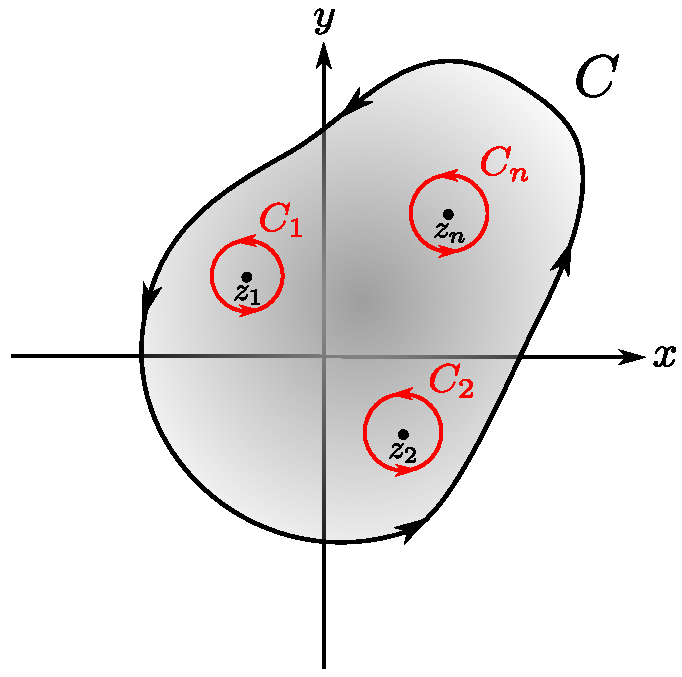
\includegraphics[scale = 0.55]{Figuras/TeoremaResiduo.pdf}
    \caption{Demostración teorema del residuo.}
    \label{fig:TeoResiduo}
\end{figure}
\end{proof}

\begin{ejemplo}
Evaluar la integral
$$\int_C \frac{5z-2}{z(z-1)} \,dz,$$

donde $C: |z| = 2$ está orientado positivamente.
\\

\textbf{Solución:} Notemos que $f(z) = \frac{5z-2}{z(z-1)}$ tiene puntos singulares aislados en $z = 0$ y $z = 1$, los cuales están en el interior de $C$. Debemos hallar los residuos de $f$ en $z = 0$ y $z = 1$, para ello usaremos la serie de Maclaurin
$$\frac{1}{1-z} = \sum_{n=0}^{\infty} z^n, \quad |z| < 1.$$

En primer lugar, escribimos el desarrollo de Laurent de $f$ en $0 < |z| < 1$:
\begin{align*}
 \frac{5z-2}{z(z-1)} = - \left( 5 - \frac{2}{z}\right) \frac{1}{1-z} &= - \left( 5 - \frac{2}{z}\right)  \sum_{n=0}^{\infty} z^n \\
 &= \sum_{n=0}^{\infty} 2z^{n-1} - \sum_{n=0}^{\infty} 5 z^n \\
 &= \frac{2}{z} - 3 - 3z - 3z^2 - \cdots 
\end{align*}

De aquí, $Res(f,0) = 2$. Por otro lado, para $0 < |z-1| < 1$, tenemos 
\begin{align*}
    \frac{5z-2}{z(z-1)} = \frac{5z-2}{z-1} \frac{1}{z} &= \frac{5z-2}{z-1} \frac{1}{1 + (z-1)} \\
    &= \frac{5z-5-2+5}{z-1} \sum_{n=0}^{\infty} (-1)^n (z-1)^n \\
    &= \left(5 + \frac{3}{z-1} \right) \sum_{n=0}^{\infty} (-1)^n (z-1)^n \\
    &=  \sum_{n=0}^{\infty} (-1)^n 5 (z-1)^n +  \sum_{n=0}^{\infty} (-1)^n 3 (z-1)^{n-1} \\
    &= \frac{3}{z-1} +2 -2(z-1) + 2(z-1)^2 - \cdots
\end{align*}

Así, $Res(f,1) = 3$. Por lo tanto,
$$\int_C \frac{5z-2}{z(z-1)} \,dz = 2\pi i\left[ Res(f,0) + Res(f,1)\right] = 10 \pi i.$$

\end{ejemplo}

\section{Ceros y polos}

\begin{defi}
Sea $f$ una función con un punto singular aislado $z_0$ y sea
$$f(z) = \sum_{n=0}^{\infty} a_n(z-z_0)^n + \sum_{n=1}^{\infty} \frac{b_n}{(z-z_0)^n}$$

su representación en serie de Laurent en un dominio $0 < |z-z_0| < R$.

\begin{enumerate}
    \item Llamaremos a:
    $$ \sum_{n=1}^{\infty} \frac{b_n}{(z-z_0)^n}$$
    
    \textbf{parte principal de $f$ en $z_0$}.
    
    \item Llamaremos a $z_0$ un \textbf{polo de orden $m$} si $b_m \neq 0$ y $b_{m+1} = b_{m+2} = \cdots = 0$. La serie de Laurent de $f$ en $z_0$ queda como sigue
    $$f(z) =  \sum_{n=0}^{\infty} a_n(z-z_0)^n +  \frac{b_1}{z-z_0} + \frac{b_2}{(z-z_0)^2} + \cdots + \frac{b_m}{(z-z_0)^m}, \quad 0 < |z-z_0| < R.$$
    
    \item Llamaremos \textbf{polo simple} si $z_0$ es un polo de orden 1.
    
    \item Llamaremos \textbf{punto singular esencial} si $b_m \neq 0$ para una infinidad de $m \in \mathbb{N}$.
    
    \item Diremos que $f$ tiene una \textbf{singularidad removible en $z_0$} si $f$ puede ser definida en $z_0$ de tal manera que sea analítica en $z_0$.
\end{enumerate}
\end{defi}

\begin{ejemplo}
La función 
$$f(z) = \frac{z^2-2z+3}{z-2}$$

tiene un polo simple en $z_0 = 2$. En efecto, si dividimos los polinomios:
\begin{figure}[H]
    \centering
    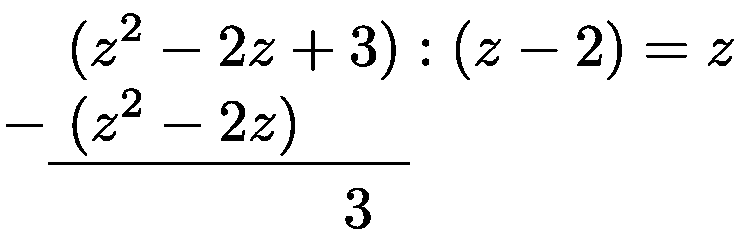
\includegraphics[scale = 0.4]{Figuras/DivisionPol.pdf}
\end{figure}

obtenemos que
$$\frac{z^2-2z+3}{z-2} = \frac{z(z-2) + 3}{z-2} = z + \frac{3}{z-2} =  (z-2) + 2 + \frac{3}{z-2}.$$
\end{ejemplo}

\begin{ejemplo}
Muestre que la función
$$f(z) = \frac{\sinh z}{z^4}$$

tiene un polo de orden $m = 3$ en $z_0 = 0$.
\\

\textbf{Solución:} Primero, determinemos la serie de Maclaurin de $\sinh z$. 

\begin{align*}
    \sinh z = \frac{e^z - e^{-z}}{2} &= \frac{1}{2} \left\{ \sum_{n=0}^{\infty} \frac{z^n}{n!} - \sum_{n=0}^{\infty} \frac{(-1)^n z^n}{n!}  \right\} \\
    &= \frac{1}{2} \sum_{n=0}^{\infty} \frac{(1-(-1)^n)}{n!} z^n \\
    &= \frac{1}{2} \sum_{k=0}^{\infty} \frac{(1-(-1)^{2k+1})}{(2k+1)!} z^{2k+1} \quad (n = 2k+1)\\
    &= \sum_{k=0}^{\infty} \frac{z^{2k+1}}{(2k+1)!}, \quad z \in \mathbb{C}.
\end{align*}

Luego,
\begin{align*}
 \frac{\sinh z}{z^4} = \sum_{k=0}^{\infty} \frac{z^{2k-3}}{(2k+1)!}& = \frac{1}{z^3} + \frac{1}{3!} \frac{1}{z} +\sum_{k=2}^{\infty} \frac{z^{2k-3}}{(2k+1)!} \\
 &=  \frac{1}{z^3} + \frac{1}{3!} \frac{1}{z} +\sum_{n=0}^{\infty} \frac{z^{2n+1}}{(2n+5)!}, \quad |z| > 0.    
\end{align*}

Claramente tiene un polo de orden 3 en $z_0 = 0$.

\end{ejemplo}

\begin{ejemplo}
La función
$$f(z) = e^{1/z} = \sum_{n=0}^{\infty} \frac{1}{n!} \frac{1}{z^n} = 1 +  \sum_{n=1}^{\infty} \frac{1}{n!} \frac{1}{z^n}, \quad |z| > 0$$

tiene un punto singular esencial en $z_0 = 0$.
\end{ejemplo}

\begin{ejemplo}
Considere la función 
$$f(z) = \frac{\sin z}{z}.$$

Sabemos que
$$\sin z = \sum_{n=0}^{\infty} \frac{(-1)^n}{(2n+1)!} z^{2n+1},$$

luego
\begin{align*}
    f(z) = \frac{\sin z}{z} &= \frac{1}{z}  \sum_{n=0}^{\infty} \frac{(-1)^n}{(2n+1)!} z^{2n+1} \\
    &= \sum_{n=0}^{\infty} \frac{(-1)^n}{(2n+1)!} z^{2n} = 1 - \frac{z^2}{3!} + \frac{z^4}{5!} - \cdots.
\end{align*}

Entonces, definiendo $f(0) = 1$, se tiene que $f$ es entera y la singularidad $z_0 = 0$ es removible. 
\end{ejemplo}

En general, si la serie de Laurent contiene sólo potencias no negativas de $z-z_0$, y la serie es, de hecho, una serie de potencias, $z_0$ es una singularidad removible. Si definimos $f$ en $z_0$ como $a_0$, la función pasa a ser analítica en $z_0$.

\begin{propo}
Sea $f$ una función analítica en una región $D$ con una singularidad aislada en $z_0$. Entonces, son equivalentes:
\begin{enumerate}
    \item $z_0$ es una singularidad removible.
    
    \item $f$ es acotada en $0 < |z-z_0| < R$.  
    
    \item $\lim\limits_{z\to z_0} f(z)$ existe.
    
    \item $\lim\limits_{z\to z_0} (z-z_0) f(z) = 0$.
\end{enumerate}
\end{propo}

\begin{proof}
\ 

\begin{itemize}
    \item  $(1) \Rightarrow (2), (3), (4)$: Supongamos que $z_0$ es una singularidad removible, se tiene que
    $$f(z) = \sum_{n=0}^{\infty} a_n (z-z_0)^n, \quad 0 < |z-z_0| < R.$$
    
    Luego, definiendo $f(z_0) = a_0$, $f$ es una función analítica en $D$. Por lo tanto, se sigue de manera inmediata (2), (3) y (4).
    
    \item $(2) \Rightarrow (4)$: Para  $0 < |z-z_0| < R$, tenemos que existe $M > 0$ tal que $|f(z)| \leq M $. Luego,
    $$|(z-z_0) f(z)| = |z-z_0| \,|f(z)| \leq M |z-z_0|.$$
    
    Por el teorema del acotamiento, cuando $z \to z_0$, tenemos que $\lim\limits_{z\to z_0} (z-z_0) f(z) = 0$.
    
    \item $(3) \Rightarrow (4)$: Por el álgebra de límites,
    $$\lim_{z\to z_0} (z-z_0) f(z) = \left( \lim_{z\to z_0} (z-z_0)  \right) \cdot \left(\lim_{z\to z_0} f(z) \right) = 0.$$
    
    \item $(4) \Rightarrow (1)$: Debemos demostrar que los $b_n = 0, n \in \mathbb{N}$. Sea $\varepsilon > 0$, existe $\delta > 0$ tal que
    $$0 < |z-z_0| < \delta \Rightarrow |f(z)| \,|z-z_0| < \varepsilon.$$
        Elijamos $r > 0$ con $r < 1$ y $r < \delta$, luego
    $$|z-z_0| = r \Rightarrow |f(z)| < \frac{\varepsilon}{|z-z_0|} = \frac{\varepsilon}{r}.$$
    
    Así,
    \begin{align*}
        |b_n| = \left| \frac{1}{2\pi i} \int_{C_r} \frac{f(\xi)}{(\xi-z_0)^{-n+1}} \,d\xi\right| &\leq \frac{1}{2\pi} \int_{C_r} |f(\xi)| \,|\xi-z_0|^{n-1} |d\xi| \\
        &< \frac{1}{2\pi} \int_{C_r} \frac{\varepsilon}{r} r^{n-1} \,|d\xi| \\
        &= \frac{1}{2\pi}\frac{\varepsilon}{r} r^{n-1} \int_{C_r}  \,|d\xi| \\
        &=  \frac{1}{2\pi}\frac{\varepsilon}{r} r^{n-1} 2\pi r \\
        &= \frac{\varepsilon}{r}r^n \leq \varepsilon.
    \end{align*}

Como $\varepsilon > 0$ es arbitrario, se concluye que, en el desarrollo de Laurent de $f$ en $z_0$, los $b_n = 0, n\in \mathbb{N}$.
\end{itemize}
\end{proof}

\begin{defi}
Sea $f$ analítica en una región $D$. Diremos que $f$ tiene un \textbf{cero de orden $m$ en $z_0$} si $f^{(i)}(z_0) = 0, i = 0,1,2, \dots, m-1$, y $f^{(m)}(z_0) \neq 0$.
\end{defi}

\begin{teorema} \label{TeoCerOrdenm}
Sea $f$ una función analítica en $z_0$. Entonces, $f$ tiene un cero de orden $m$ en $z_0$ si y sólo si $f(z)$ puede ser escrita como
\begin{equation}
 f(z) = (z-z_0)^m g(z),   \label{CerosOrdenm}
\end{equation}

donde $g$ es analítica en $z_0$ y $g(z_0) \neq 0$.
\end{teorema}

\begin{proof}
Dado que $f$ es analítica en $z_0$, entonces puede ser expandida en una serie de Taylor, es decir,
$$f(z) = \sum_{n=0}^{\infty} \frac{f^{(n)}(z_0)}{n!} (z-z_0)^n$$

en algún disco $B(z_0,R)$. Si $f$ tiene un cero de orden $m$ en $z_0$, entonces $f^{(i)}(z_0) = 0, i = 0,1,2, \dots, m-1$, y $f^{(m)}(z_0) \neq 0$. Por lo tanto, la serie de Taylor se reduce a 
$$f(z) = \sum_{n=m}^{\infty} \frac{f^{(n)}(z_0)}{n!} (z-z_0)^n = (z-z_0)^m \sum_{n=m}^{\infty} \frac{f^{(n)}(z_0)}{n!} (z-z_0)^{n-m}.$$

Como las series de potencias convergentes representan siempre funciones analíticas, podemos escribir
$$f(z) = (z-z_0)^m g(z),$$

donde $g$ es analítica en $|z-z_0| < R$ y $g(z_0) \neq 0$.

Por otro lado, supongamos que $f(z) = (z-z_0)^m g(z)$. Como $g$ es analítica en $z_0$, tiene una expansión en serie de Taylor 
$$g(z) = \sum_{n=0}^{\infty} b_n (z-z_0)^n,$$

ya que $g(z_0) \neq 0$, se sigue que $b_0 \neq 0$. Por lo tanto,
$$f(z) =  (z-z_0)^m  \sum_{n=0}^{\infty} b_n (z-z_0)^n = \sum_{n=0}^{\infty} b_n (z-z_0)^{m+n},$$

lo cual implica que $f$ tiene un cero de orden $m$ en $z_0$.

\end{proof}

Un teorema similar se tiene para los polos de orden $m$.

\begin{teorema} \label{TeoPoloOrdenm}
Una función $f$ tiene un polo de orden $m$ en $z_0$ si y sólo si, en alguna vecindad, sin su centro, de $z_0$,
\begin{equation}
f(z) = \frac{\phi(z)}{(z-z_0)^m},    \label{PoloOrdenm}
\end{equation}

donde $\phi$ es analítica en $z_0$ y $\phi(z_0) \neq 0$
\end{teorema}

\begin{proof}
 Supongamos que $f$ tiene un polo de orden $m$ en $z_0$, entonces su representación en serie de Laurent está dada por
\begin{align*}
 f(z) &= \frac{b_m}{(z-z_0)^m} + \cdots + \frac{b_1}{z-z_0} + \sum_{n=0}^{\infty} a_n (z-z_0)^n \\
 &= \frac{1}{(z-z_0)^m} \left\{ b_m + b_{m-1} (z-z_0) + \cdots + b_1 (z-z_0)^{m-1} + \sum_{n=0}^{\infty} a_n (z-z_0)^{n+m} \right\},
\end{align*}

para alguna región anular $0 < |z-z_0| < R$ y $b_m \neq 0$. Como lo que está entre corchetes es una serie de potencias, podemos escribir
\begin{equation*}
f(z) = \frac{\phi(z)}{(z-z_0)^m}, 
\end{equation*}

donde $\phi$ es analítica en $z_0$ y $\phi(z_0) = b_m \neq 0$. 

Por otro lado, supongamos que $f(z) = \phi(z)/(z-z_0)^m$, donde  $\phi$ es analítica en $z_0$ y $\phi(z_0) \neq 0$, entonces, por el teorema de Taylor,
$$g(z) = \sum_{n=0}^{\infty} c_n (z-z_0)^n, \quad c_0 = \phi(z_0) \neq 0.$$

Así, la serie de Laurent de $f$ alrededor de $z_0$ es
$$f(z) = \frac{1}{(z-z_0)^m} \sum_{n=0}^{\infty} c_n (z-z_0)^n = \frac{c_0}{(z-z_0)^m} + \frac{c_1}{(z-z_0)^{m-1}} + \cdots .$$

Como $c_0 \neq 0$, $z_0$ es un polo de orden $m$ para $f$.

\end{proof}

Las ceros y polos de una función está relacionados mediante el siguiente teorema.

\begin{teorema} \label{CeroYPolos}
Si $f$ es analítica en una vecindad de $z_0$, entonces $f$ tiene un cero de orden $m$ en $z_0$ si, y sólo si, $1/f$ tiene un polo de orden $m$ en $z_0$.
\end{teorema}

\begin{proof}
Supongamos que $m$ tiene un cero de orden $m$ en $z_0$, probemos que $1/f$ tiene un polo de orden $m$ en $z_0$. 

Usando \eqref{CerosOrdenm}, podemos escribir $f(z) = (z-z_0)^m g(z)$, con $g$ analítica en $z_0$ y $g(z_0) \neq 0$, por tanto, $g(z) \neq 0$ en una vecindad de $z_0$. En efecto, como analiticidad implica continuidad, tenemos
$$\lim_{z\to z_0} g(z) = g(z_0).$$

Para $\varepsilon = \frac{1}{2} g(z_0)$, existe $\delta >0$ tal que
$$0 < |z-z_0| < \delta \Rightarrow |g(z) - g(z_0)| < \frac{1}{2} g(z_0) \Leftrightarrow \frac{1}{2} g(z_0) < g(z) < \frac{3}{2} g(z_0).$$

Luego, $h(z) = \frac{1}{g(z)}$ es analítica en tal vecindad, ésto es,
$$\frac{1}{g(z)} = \sum_{n=0}^{\infty} a_n (z-z_0)^n, \quad |z-z_0| < \delta.$$

Entonces,
\begin{align*}
  \frac{1}{f(z)} &= \frac{1}{(z-z_0)^m}  \sum_{n=0}^{\infty} a_n (z-z_0)^n \\
  &=   \sum_{n=0}^{\infty} a_n (z-z_0)^{n-m} \\
  &= \frac{a_0}{(z-z_0)^{m}} + \frac{a_1}{(z - z_0)^{m-1}} + \cdots + \frac{a_{m-1}}{z-z_0} +  \sum_{n=m}^{\infty} a_n (z-z_0)^{n-m} \\
  &=  \frac{a_0}{(z-z_0)^{m}} + \frac{a_1}{(z - z_0)^{m-1}} + \cdots + \frac{a_{m-1}}{z-z_0} +  \sum_{n=0}^{\infty} a_{n+m} (z-z_0)^{n}.
\end{align*}

Por lo tanto, $\frac{1}{f(z)}$ tiene un polo de orden $m$.

Por otro lado, supongamos que $1/f$ tiene un polo de orden $m$ en $z_0$, usando \eqref{PoloOrdenm}, podemos escribir
\begin{equation*}
\frac{1}{f(z)} = \frac{\phi(z)}{(z-z_0)^m}, 
\end{equation*}

donde $\phi$ es analítica en $z_0$ y $\phi(z_0) \neq 0$, por tanto, $\phi(z) \neq 0$ en una vecindad de $z_0$. Luego, $\frac{1}{\phi(z)}$ es analítica en tal vecindad, ésto es,
$$\frac{1}{\phi(z)} = \sum_{n=0}^{\infty} c_n(z-z_0)^n, \quad |z-z_0| < \delta^*.$$

Entonces,
$$  f(z) = (z-z_0)^m  \sum_{n=0}^{\infty} c_n(z-z_0)^n =   \sum_{n=0}^{\infty} c_n (z-z_0)^{n+m}= \sum_{n=m}^{\infty} c_{n-m} (z-z_0)^n.$$

Lo que implica, por el teorema de Taylor, que
$$f^{(n)}(z_0) \neq 0, \quad n \geq m~~\mbox{y}~~ f^{(n)}(z_0) = 0, \quad n < m,$$

es decir, $f$ tiene un cero de orden $m$ en $z_0 = 0$.
\end{proof}

\section{Cálculo de residuos}

Hasta hora hemos determinado los residuos de una función encontrando su serie de Laurent, pero ésto no es necesario como lo veremos a continuación. 

\begin{teorema}
Sea $f$ una función analítica en una región $D$ con una singularidad aislada en $z_0$. Son equivalentes:
\begin{enumerate}
    \item $z_0$ es polo simple de $f$.
    
    \item $\lim\limits_{z\to z_0} (z-z_0) f(z) = b_1 \neq 0$.
\end{enumerate}
\end{teorema}

\begin{proof}
$z_0$ es un polo simple si y sólo si la serie de Laurent en $z_0$ tiene la forma
$$f(z) = \frac{b_1}{z-z_0} + a_0 + a_1 (z-z_0) + a_2(z-z_0)^2 + \cdots = \frac{b_1}{z-z_0} + g(z),$$

donde $b_1 \neq 0$ y $g$ es la serie de potencia analítica parte de la serie de Laurent. Entonces,
\begin{align*}
 (z-z_0)f(z) = b_1 + (z-z_0)g(z) \Leftrightarrow \lim_{z\to z_0} (z-z_0) f(z) &= b_1 + \left( \lim_{z\to z_0} (z-z_0)\right) \left(\lim_{z\to z_0} g(z) \right) \\
 &= b_1 + 0 a_0 = b_1.   
\end{align*}

\end{proof}

\begin{ejemplo}
Sea $C$ una curva simple cerrada orientada positivamente tal que $1$, $-i$ e $i$ están en su exterior y $-1$ en su exterior. Evaluar
$$\int_C \frac{1}{z^4+1} \,dz.$$

\textbf{Solución:} Notemos que
$$f(z) = \frac{1}{z^4+1} = \frac{1}{(z-1)(z+1)(z+i)(z-i)}.$$

Luego, la función $f$ tiene singularidades aisladas en $z = \pm 1, \pm i$. Tres de estas están en el interior de $C$, entonces, por el teorema del residuo,
$$\int_C \frac{1}{z^4+1} \,dz = 2\pi i \left[ Res(f,1) + Res(f,i) + Res(f,-i)\right].$$

Supongamos que tiene polos simples. Calculemos:
\begin{align*}
    \lim_{z\to 1} (z-1) \frac{1}{(z^4+1)}&= \lim_{z\to 1} \frac{1}{(z+1)(z-i)(z+i)} \\
    &= \left. \frac{1}{(z+1)(z-i)(z+i)} \right|_{z=1} \\
    &= \frac{1}{4}, \\
    \lim_{z\to i} (z-i) \frac{1}{(z^4+1)}&= \lim_{z\to i} \frac{1}{(z-1)(z+1)(z+i)} \\
    &= \left. \frac{1}{(z-1)(z+1)(z+i)} \right|_{z=i} \\
    &= \frac{i}{4} , \\
     \lim_{z\to -i} (z+i) \frac{1}{(z^4+1)}&= \lim_{z\to -i} \frac{1}{(z-1)(z+1)(z-i)} \\
    &= \left. \frac{1}{(z-1)(z+1)(z-i)} \right|_{z=-i} \\
    &= -\frac{i}{4}. 
\end{align*}

Como todos estos límites son distintos de cero, $z = 1,\pm i$ son polos simples de $f$ y
$$Res(f,1) = \frac{1}{4},~ Res(f,i) = \frac{i}{4}, ~ Res(f,-i) = - \frac{i}{4}.$$

Por lo tanto,
$$\int_C \frac{1}{z^4+1} \,dz = 2\pi i \left[ \frac{1}{4} + \frac{i}{4} - \frac{i}{4}\right] = \frac{\pi i}{2}.$$
\end{ejemplo}

Para polos de orden mayor, se tiene el siguiente teorema.

\begin{teorema}
Supongamos que $z_0$ es un polo de orden $m \geq 1$ de $f$. Entonces,
$$Re(f,z_0) = \lim_{z\to z_0} \frac{1}{(m-1)!} \frac{d^{m-1}}{dz^{m-1}}[(z-z_0)^m f(z)].$$
\end{teorema}

\begin{proof}
Como $z_0$ es un polo de orden $m\geq 1$ de $f$, entonces su serie de Laurent en $z_0$ tiene la forma
$$f(z) = \frac{b_m}{(z-z_0)^m} + \cdots + \frac{b_1}{z-z_0} + \sum_{n=0}^{\infty} a_n (z-z_0)^n.$$

Multiplicando por $(z-z_0)^m$, luego derivando $(m-1)$ veces, obtenemos
$$\frac{d^{m-1}}{dz^{m-1}}[(z-z_0)^m f(z)] = (m-1)! b_1 + \sum_{n=0}^{\infty} \frac{(n+m)!}{(n+1)!} a_n (z-z_0)^{n+1}.$$

Tomando el límite cuando $z\to z_0$, tenemos
$$\lim_{z\to z_0}  \frac{d^{m-1}}{dz^{m-1}}[(z-z_0)^m f(z)] = (m-1)! b_1 + 0.$$

Lo que implica que
$$\lim_{z\to z_0} \frac{1}{(m-1)!} \frac{d^{m-1}}{dz^{m-1}}[(z-z_0)^m f(z)] = b_1.$$
\end{proof}


\begin{ejemplo}
Determine el residuo de 
$$f(z) = \frac{z^2}{(z^2+\pi^2)^2 \sin z}$$

en $z_0 = i\pi$.
\\

\textbf{Solución:} La función $f$ es analítica excepto cuando $z^2 + \pi^2 = 0$ o $\sin z = 0$. Por lo tanto, $f$ tiene singularidades aisladas en $\pm i \pi$ y en $k\pi$ con $k \in \mathbb{Z}$. Para determinar el residuo de $f$ en $z_0 = i\pi$, consideremos la función
$$\frac{1}{f(z)} = \frac{(z+i\pi)^2 (z-i\pi)^2 \sin z}{z^2} = (z-i\pi)^2 \frac{(z+i\pi)^2 \sin z}{z^2},$$

la cual tiene la forma
$$(z-i\pi)^2 g(z)$$

con $g$ analítica en $z_0= i\pi $ y $g(z_0) \neq i\pi$. Luego, $1/f$ tiene un cero de orden 2 en $i\pi$. Entonces, por el teorema \ref{CeroYPolos}, $f$ tiene un polo de orden $2$. Así,
\begin{align*}
    Res(f,i\pi) &= \lim_{z\to i\pi} \frac{d}{dz} [(z-i\pi)^2 f(z)] \\
    &= \lim_{z\to i\pi} \frac{d}{dz} \left[\frac{z^2}{(z+i\pi)^2 \sin z}\right]  \\
    &= \lim_{z\to i\pi} \frac{2z(z+i\pi)\sin z - z^2 ((z+i\pi) \cos z + 2\sin z)}{(z+i\pi)^3 \sin^2(z)} \\
    &= \frac{2\sinh(\pi) + (-\pi \cosh(\pi) - \sinh(z))}{-4\pi \sinh^2(\pi)} = - \frac{1}{4\pi \sinh(\pi)} + \frac{\cosh(\pi)}{4\pi \sinh^2(\pi)}.
\end{align*}

\end{ejemplo}

\begin{propo}
Sean $g$ y $h$ analíticas en $z_0$ y suponga que $g(z_0) \neq 0$, $h(z_0) = 0$ y $h'(z_0) \neq 0$. Entonces, $f(z) = g(z)/h(z)$ tiene un polo simple en $z_0$, y
$$Res(f,z_0) = \frac{g(z_0)}{h'(z_0)}.$$
\end{propo}

\begin{proof}
Sabemos que
$$\lim_{z\to z_0} \frac{h(z) - h(z_0)}{z-z_0} = \lim_{z\to z_0} \frac{h(z)}{z-z_0} = h'(z_0) \neq 0.$$

Entonces,
$$\lim_{z\to z_0} \frac{z-z_0}{h(z)} = \frac{1}{h'(z_0)}.$$

Así,
$$\lim_{z\to z_0} (z-z_0) f(z) = \lim_{z\to z_0} (z-z_0) \frac{g(z)}{h(z)} = \frac{g(z_0)}{h'(z_0)}$$

existe y es distinto de cero. Por lo tanto, $f$ tiene un polo simple y 
$$Res(f,z_0) = \frac{g(z_0)}{h'(z_0)}.$$
\end{proof}

\section{Integrales reales impropias}

En esta sección se entregará una técnica útil para evaluar integrales impropias del tipo
$$\int_{-\infty}^b f(x) \,dx ~~\mbox{y}~~ \int_a^{\infty} f(x) \,dx, \quad a,b \in \mathbb{R},$$

donde $f$ es continua en todo intervalo cerrado dentro del intervalo de integración. Además, de
$$\int_{-\infty}^{\infty} f(x)\,dx$$

donde $f$ es continua en $\mathbb{R}$.

Sabemos del cálculo integral de una variable que $\int_{-\infty}^{\infty} f(x)\,dx$ converge si
$$\lim_{a \to - \infty} \int_{a}^{0}f(x) \,dx; \quad \lim_{b \to + \infty} \int_{0}^{b}f(x) \,dx$$

existen y, en tal caso,
$$\int_{-\infty}^{\infty} f(x) \,x = \lim_{a \to - \infty} \int_{a}^{0}f(x) \,dx +  \lim_{b \to + \infty} \int_{0}^{b}f(x) \,dx .$$

\begin{defi}
Definimos el \textbf{valor principal de Cauchy} de la integral $\int_{-\infty}^{\infty} f(x)\,dx$ a
$$V.P. \int_{- \infty}^{\infty} f(x) \,dx = \lim_{a\to + \infty} \int_{-a}^a f(x)\,dx$$

si el límite existe.
\end{defi}

\textbf{Observación:} El valor principal de Cauchy de una integral puede existir incluso cuando la integral en si misma no es convergente. Por ejemplo, $\int_{-a}^ax dx = 0$ para todo $a$, lo cual implica que $V.P. \int_{-\infty}^{\infty} xdx = 0$, pero la integral en si no converge, pues $\int_0^{\infty} xdx = \infty$. Sin embargo, 
$$\int_{\infty}^{\infty} f(x) \,dx < \infty \Rightarrow V.P. \int_{\infty}^{\infty} f(x) \,dx < \infty$$

y ambas integrales coinciden. En efecto, los límites
$$\lim_{a \to \infty} \int_{-a}^{0}f(x) \,dx; \quad \lim_{a \to + \infty} \int_{0}^{a}f(x) \,dx$$

existen y
\begin{align*}
   V.P. \int_{- \infty}^{\infty} f(x) \,dx &= \lim_{a\to + \infty} \int_{-a}^a f(x)\,dx  \\
   &= \lim_{a\to + \infty} \left(\int_{-a}^{0} f(x) \,dx + \int_0^a f(x) \,dx \right) \\
   &= \lim_{a\to + \infty} \int_{-a}^{0} f(x) \,dx +  \lim_{a\to + \infty}\int_0^a f(x) \,dx \\
   &= \int_{- \infty}^{+\infty} f(x) \,dx.
\end{align*} 

Pero supongamos que $f$ es una función par, es decir, $f(-x) = f(x)$ para todo $x \in \mathbb{R}$. Entonces, si el valor principal de Cauchy existe, la integral converge al mismo valor (demuéstrelo!!!!!). De hecho,
\begin{equation}
 \int_0^{+\infty} f(x) \,dx = \frac{1}{2} \int_{-\infty}^{+ \infty} f(x) \,dx. \label{IntIPar}   
\end{equation}

Nuestro propósito será calcular el V.P. Para ilustrar el método, analicemos el siguiente ejemplo.

\begin{ejemplo} \label{EjImpropia1}
Calcular 
$$\int_0^{\infty} \frac{2x^2-1}{x^4+5x^2+4} \,dx.$$

\textbf{Solución:} La función
$$f(x) =  \frac{2x^2-1}{x^4+5x^2+4}$$

es continua en $\mathbb{R}$ y es una función par. Luego,
$$\int_0^{\infty} \frac{2x^2-1}{x^4+5x^2+4} \,dx = \frac{1}{2} \int_{-\infty}^{\infty} \frac{2x^2-1}{x^4+5x^2+4} \,dx.$$

Extendamos la función $f$ a todo $\mathbb{C}$, 
$$f(z) = \frac{2z^2-1}{z^4+5z^2+4} = \frac{2z^2-1}{(z^2+1)(z^2+4)},$$

excepto para los puntos donde $z^4+5z^2+4 = 0$; $\pm i, \pm 2 i$. Consideremos la curva simple cerrada suave por tramos $\gamma = C_R + S_{-R,R}$ orientada positivamente, donde $R > 2$ (para que las singularidades estén dentro de $\gamma$), $C_R$ es la semicircunferencia $|z| = R$ y $S_{-R,R}$ es el segmento dirigido de $-R$ a $R$ (ver figura \ref{fig:IntegralImpropia1}).

\begin{figure}[H]
    \centering
    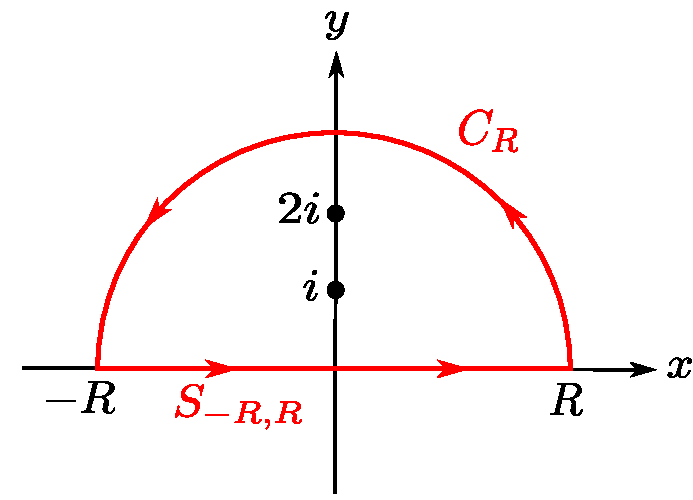
\includegraphics[scale = 0.6]{Figuras/IntegralImpropia1.pdf}
    \caption{La curva de integración para el ejemplo \ref{EjImpropia1}.}
    \label{fig:IntegralImpropia1}
\end{figure}

Por el teorema de residuos,
$$\int_{\gamma} f(z) \,dz = 2\pi i [Res(f,i) + Res(f,2i)].$$

Pero,
$$\int_{\gamma} f(z) \,dz = \int_{-R}^R f(x) \,dx + \int_{C_R}f(z)\,dz.$$

De acuerdo al cálculo de residuos,
\begin{align*}
    Res(f,i) &= \lim_{z\to i} (z-i)f(z) = \frac{i}{2}, \\
    Res(f,2i) &= \lim_{z\to 2i} (z-2i)f(z) = -\frac{3i}{4}.
\end{align*}

Por lo tanto,
$$\int_{-R}^R f(x) \,dx + \int_{C_R}f(z)\,dz = 2\pi i \left[\frac{i}{2} - \frac{3i}{4}\right] = \frac{\pi}{2}.$$

Lo que implica
$$\int_{-R}^R f(x) \,dx = \frac{\pi}{2} - \int_{C_R}f(z)\,dz.$$

Queda por analizar el comportamiento de $\int_{C_R} f(z) \,dz$. Para ello, notemos que para $|z| = R$:
$$|2z^2-1| \leq 2|z|^2 +1 = 2R^2+1$$

y
$$|z^4+5z^2+4| = |z^2+1|\,|z^2+4| \geq ||z|^2 - 1|\,||z|^2-4| = (R^2-1)(R^2-4).$$

Entonces, para cualquier $z \in C_R$,
$$\left| \frac{2z^2-1}{z^4+5z^2+4} \right| \leq \frac{2R^2+1}{(R^2-1)(R^2-4)}$$

y ésto significa que 
$$\left|\int_{C_R} f(z) \,dz \right| \leq\frac{2R^2+1}{(R^2-1)(R^2-4)} \pi R.$$

Como
$$\lim_{R \to + \infty} \frac{2R^2+1}{(R^2-1)(R^2-4)} \pi R = 0 \Rightarrow \lim_{R \to + \infty} \int_{C_R} f(z) \,dz = 0.$$

Así,
$$\lim_{R \to + \infty} \int_{-R}^R f(x) \,dx = \frac{\pi}{2} - \lim_{R\to + \infty} \int_{C_R} f(z) \,dz = \frac{\pi}{2},$$

o sea
$$V.P. \int_{-\infty}^{\infty}  \frac{2x^2-1}{x^4+5x^2+4} \,dx = \frac{\pi}{2}.$$

Como el integrando es par, sabemos que la integral converge a su valor principal de Cauchy, y de acuerdo con la ecuación \eqref{IntIPar},
$$\int_0^{\infty} \frac{2x^2-1}{x^4+5x^2+4} \,dx = \frac{1}{2}  \int_{-\infty}^{\infty}  \frac{2x^2-1}{x^4+5x^2+4} \,dx = \frac{\pi}{4}.$$

Se obtiene el mismo resultado al tomar la semicircunferencia por debajo del eje real ($Im(z) < 0$), pero para que coincidan los signos, la orientación debe ser negativa.
\end{ejemplo}

El procedimiento anterior funciona siempre y cuando se satisfagan las hipótesis del siguiente teorema.

\begin{teorema}
Sea $f$ una función analítica con un número finito de puntos singulares aislados $z_1, \dots, z_n$, todos ellos ubicados en la región $Im (z) > 0$. Entonces,
$$\lim_{R\to + \infty} \sup_{|z| \leq R} |zf(z)| = 0 \Rightarrow \lim_{R\to + \infty} \int_{-R}^R f(x) \,dx = 2\pi i \sum_{i=1}^n Res(f,z_i).$$
\end{teorema}

\begin{proof}
Sea $\gamma = C_R + S_{-R,R}$ una curva cerrada, suave a trazos orientada positivamente con $R > \max\{|z_i| : i = 1,2, \dots, n\}$, como en la figura,

\begin{figure}[H]
    \centering
    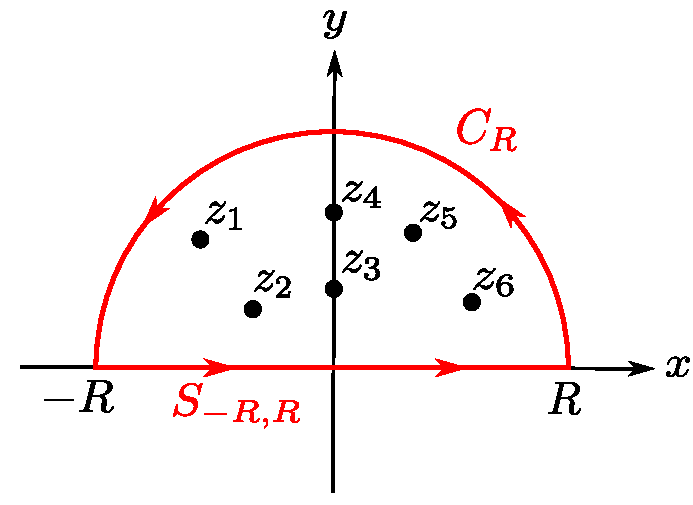
\includegraphics[scale = 0.6]{Figuras/IntegralImpropia2.pdf}
    \caption{La curva de integración para la demostración del teorema.}
    \label{fig:IntegralImpropia2}
\end{figure}

Por el teorema del residuo, tenemos que
$$\int_{\gamma} f(z)\,dz = 2\pi i \sum_{i=1}^n Res(f,z_i).$$

Ahora, 
\begin{align*}
    \int_{\gamma} f(z) \,dz &= \int_{-R}^R f(x) \,dx + \int_{C_R} f(z) \,dz \\
    \Rightarrow \int_{-R}^R f(x) \,dx &=  2\pi i \sum_{i=1}^n Res(f,z_i) - \int_{C_R} f(z) \,dz.
\end{align*}

Como $f$ es continua en $C_R$, $|f(z)|$ está acotada tal que
$$\forall z \in C_R: ~ |f(z)| \leq \sup_{z \in C_R} |f(z)| < \infty.$$

Luego,
$$\left| \int_{C_R} f(z) \,dz \right| \leq \pi R \sup_{z \in C_R} |f(z)|.$$

Por propiedades del supremo y teniendo en cuenta que estamos estudiando la integral para los $|z| = R$, se tiene que
$$R \sup_{z \in C_R} |f(z)| = \sup_{z \in C_R} R |f(z)| =\sup_{z \in C_R} |z f(z)|.$$

Entonces,
$$\left| \int_{C_R} f(z) \,dz \right| \leq \pi \sup_{z \in C_R} |zf(z)|.$$

Por hipótesis,
$$\lim_{R\to + \infty} \sup_{|z| \leq R} |zf(z)| = 0  \Rightarrow  \int_{C_R} f(z) \,dz  = 0.$$

Por lo tanto,
$$\lim_{R \to + \infty} \int_{-R}^R f(x) \,dx = 2\pi i \sum_{i=1}^n Res(f,z_i) - \lim_{R\to + \infty} \int_{C_R} f(z) \,dz = 2\pi i \sum_{i=1}^n Res(f,z_i).$$
\end{proof}

Ahora nos centraremos en calcular integrales impropias convergentes del tipo
$$\int_{-\infty}^{\infty} f(x) \sin(ax) \,dx ~~\mbox{y}~~ \int_{-\infty}^{\infty} f(x) \cos(ax) \,dx$$

donde $a$ denota una constante positiva. El método descrito anteriormente no es aplicable directamente, pues $\sin z$ y $\cos z$ crecen como $\sinh y$ o $e^{ay}$, al tender $y$ al infinito. La modificación se ilustra en el siguiente ejemplo.

\begin{ejemplo} \label{EjImpropia2}
Calcular la integral impropia
$$\int_{- \infty}^{\infty} \frac{\cos(x)}{1+x^2} dx.$$

\textbf{Solución:} La integral es convergente, pues
$$\forall x \in \mathbb{R}: ~\left| \frac{\cos(x)}{1+x^2} \right| \leq \frac{1}{1+x^2}$$

y
$$\int_{-\infty}^{\infty} \frac{1}{1+x^2} \,dx = \pi.$$

Para determinar su valor, consideremos la integral compleja
$$\int_{\gamma} \frac{e^{iz}}{1+z^2} \,dz,$$

donde $\gamma = C_R + S_{-R,R}$ orientada positivamente con $R > 1$ (ver figura \ref{fig:IntegralImpropia3}). El integrando tiene solo la singularidad aislada $z = i$ dentro de la curva de integración. Entonces, por el teorema del residuo,
$$\int_{\gamma} \frac{e^{iz}}{1+z^2} \,dz = \int_{-R}^R \frac{e^{ix}}{1+x^2} \,dx + \int_{C_R} \frac{e^{iz}}{1+z^2} \,dz = 2\pi i Res(f,i).$$

\begin{figure}[H]
    \centering
    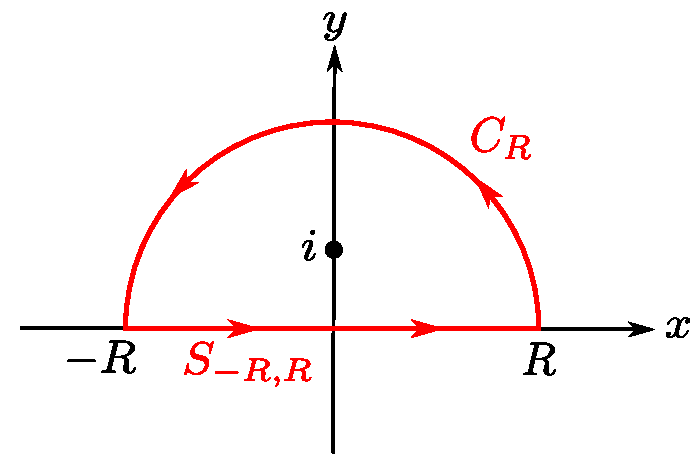
\includegraphics[scale = 0.6]{Figuras/IntegralImpropia3.pdf}
    \caption{La curva de integración para el ejemplo \ref{EjImpropia2}.}
    \label{fig:IntegralImpropia3}
\end{figure}

Ahora,
$$Res(f,i) = \lim_{z\to i} (z-i) \frac{e^{iz}}{1+z^2} = \lim_{z\to i} \frac{e^{iz}}{z+i} = - \frac{1}{2} i e^{-1}.$$

Así,
$$ \int_{-R}^R \frac{e^{ix}}{1+x^2} \,dx = \frac{\pi}{e} - \int_{C_R} \frac{e^{iz}}{1+z^2} \,dz.$$

Acotando el integrando sobre $C_R$:
$$\forall z \in C_R: ~ \left| \frac{e^{iz}}{1+z^2} \right| \leq \frac{1}{|1 - |z|^2|} = \frac{1}{R^2-1}.$$

Luego,
$$\left|\int_{C_R} \frac{e^{iz}}{1+z^2}\right| \leq \frac{1}{R^2-1} \pi R.$$

Como
$$\lim_{R\to + \infty} \frac{\pi R}{R^2-1} = 0 \Rightarrow \lim_{R\to + \infty} \int_{C_R} \frac{e^{iz}}{1+z^2} = 0.$$

Por lo tanto,
$$\lim_{R \to + \infty} \int_{-R}^R \frac{e^{ix}}{1+x^2} \,dx = \frac{\pi}{e} - \lim_{R\to + \infty} \int_{C_R} f(z) \,dz =  \frac{\pi}{e}.$$

Pero,
$$\int_{-R}^R \frac{e^{ix}}{1+x^2} \,dx = \int_{-R}^R \frac{\cos(x)}{1+x^2} \,dx + i \int_{-R}^R \frac{\sin x}{1+x^2} \,dx.$$

Como
$$\int_{-R}^R \frac{\sin(x)}{1+x^2} \,dx = 0 \quad  \mbox{(Integrando impar)},$$

tenemos que
$$\lim_{R \to + \infty} \int_{-R}^R \frac{e^{ix}}{1+x^2} \,dx = \lim_{R \to + \infty} \int_{-R}^R \frac{\cos(x)}{1+x^2} \,dx = \frac{\pi}{e}.$$

Como el integrando es par,
$$\int_{-\infty}^{\infty}\frac{\cos(x)}{1+x^2} \,dx = \frac{\pi}{e}. $$

\end{ejemplo}

\begin{lema}[Lema de Jordan]
La siguiente desigualdad es válida para $a > 0$:
$$\int_{0}^{\pi} e^{-a \sin \theta} d\theta \leq \frac{\pi}{a}.$$
\end{lema}

\begin{proof}
Comenzamos escribiendo
$$\int_0^{\pi} e^{-a \sin \theta} d\theta = \int_0^{\pi/2} e^{-a \sin \theta} d\theta + \int_{\pi/2}^{\pi} e^{-a \sin \theta} d\theta.$$

Haciendo el cambio de variable $u = \pi - \theta \Rightarrow du = -d\theta$ en la segunda integral y notando que $\sin (\theta) = \sin(\pi - u) =  \sin(u)$, obtenemos
\begin{equation}
\int_0^{\pi} e^{-a \sin \theta} d\theta = \int_0^{\pi/2} e^{-a \sin \theta} d\theta - \int_{\pi/2}^{0} e^{-a \sin u} d u = 2 \int_0^{\pi/2} e^{-a \sin \theta} d\theta.    \label{Jordan1}
\end{equation}

Probemos la desigualdad de Jordan:
\begin{equation}
\forall \theta \in [0, \pi/2]:~ \sin \theta \geq \frac{2}{\pi} \theta.    \label{DesiJordan}
\end{equation}

Para ello, consideremos la integral
$$\int_0^1 \left[\cos(\theta x) - \cos\left( \frac{\pi x }{2}\right)\right]\,dx, \quad  \theta \in ]0,2\pi[.$$

la cual representa el área entre las curvas $\cos(\theta x)$ y $\cos\left( \frac{\pi x}{2}\right)$ en $[0,1]$. Como este integral es positiva,
$$\int_0^1 \left[\cos(\theta x) - \cos\left( \frac{\pi x }{2}\right)\right] = \frac{\sin \theta}{\theta} - \frac{2}{\pi} \geq 0 \Rightarrow \sin \theta \geq \frac{2\theta}{\pi} .$$

La desigualdad \eqref{DesiJordan} implica que $-a \sin \theta \leq - \frac{2}{\pi} a \theta$ y combinado esto con \eqref{Jordan1}, deducimos que
$$\int_{0}^{\pi} e^{-a \sin \theta} \,d \theta \leq 2 \int_{0}^{\pi/2} e^{- \frac{2}{\pi} a \theta} \,d\theta = \left. - \frac{\pi}{a} e^{-\frac{2}{\pi} a\theta}\right|_{0}^{\pi/2} = \frac{\pi}{a}(1-e^{-a}) \leq \frac{\pi}{a}.$$
\end{proof}

\begin{teorema}
Sea $f$ una función analítica con un número finito de puntos singulares aislados $z_1, \dots, z_n$, todos ellos ubicados en la región $Im(z) > 0$. Entonces,
$$\lim_{R\to + \infty} \sup_{|z| \leq R} |f(z)| = 0 \Rightarrow \lim_{R\to + \infty} \int_{-R}^R f(x) e^{i\alpha x}\,dx = 2\pi i \sum_{i=1}^n Res(f(z) e^{i\alpha z},z_i), \quad \alpha > 0.$$
\end{teorema}

\begin{proof}
Sea $\gamma = C_R + S_{-R,R}$ una curva cerrada, suave a trazos orientada positivamente con $R > \max\{|z_i| : i = 1,2, \dots, n\}$, como en la figura,

\begin{figure}[H]
    \centering
    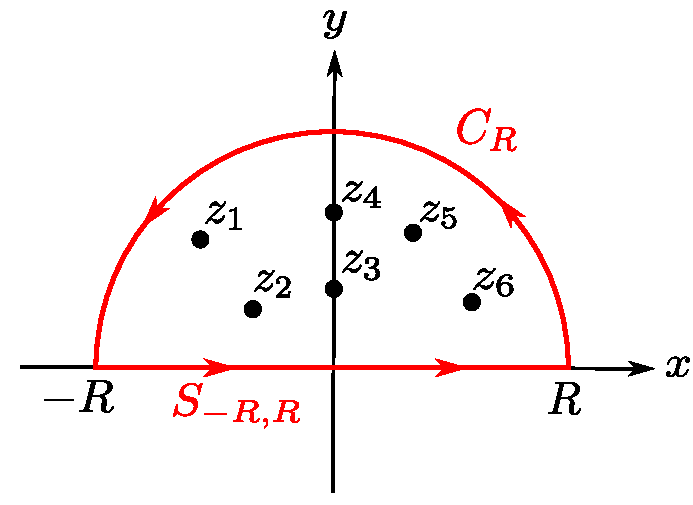
\includegraphics[scale = 0.6]{Figuras/IntegralImpropia2.pdf}
    \caption{La curva de integración para la demostración del teorema.}
    \label{fig:IntegralImpropia6}
\end{figure}

Por el teorema del residuo, tenemos que
$$\int_{\gamma} f(z) e^{i\alpha z}\,dz = 2\pi i \sum_{i=1}^n Res(f(z) e^{i\alpha z},z_i).$$

Ahora, 
\begin{align*}
    \int_{\gamma} f(z) e^{i\alpha z} \,dz &= \int_{-R}^R f(x) e^{i\alpha x} \,dx + \int_{C_R} f(z)  e^{i\alpha z} \,dz \\
    \Rightarrow \int_{-R}^R f(x) e^{i\alpha x}\,dx &=  2\pi i \sum_{i=1}^n Res(f(z) e^{i\alpha z},z_i) - \int_{C_R} f(z)  e^{i\alpha z} \,dz.
\end{align*}

Como $f$ es continua en $C_R$, $|f(z)|$ está acotada tal que
$$\forall z \in C_R: ~ |f(z)| \leq \sup_{z \in C_R} |f(z)| = M(R) < \infty.$$

Luego,
\begin{align*}
 \left| \int_{C_R} f(z) e^{i\alpha z} \,dz \right| &=  \left| \int_0^{\pi} f(R e^{i\theta}) e^{i \alpha R e^{i\theta}} i Re^{i\theta}d\theta \right| \\
 &\leq \int_0^{\pi}|f(R e^{i\theta})| \, \left|e^{i \alpha R (\cos \theta + i \sin \theta)} \right| \,|i Re^{i\theta}|\,d\theta \\
 &\leq \int_0^{\pi} M(R) e^{-\alpha R\sin\theta} R \,d\theta \\
 &= R M(R) \int_0^{\pi} e^{-\alpha R\sin\theta} \,d\theta \\
 &\leq R M(R) \frac{\pi}{\alpha R} = \frac{\pi}{\alpha} M(R).
\end{align*}

Por hipótesis,
$$\lim_{R\to + \infty} \sup_{|z| \leq R} |f(z)| = 0  \Rightarrow \lim_{R \to + \infty} \int_{C_R} f(z) e^{i\alpha z} \,dz   = 0.$$

Por lo tanto,
\begin{align*}
\lim_{R\to + \infty} \int_{-R}^R f(x) e^{i\alpha x}\,dx &= 2\pi i \sum_{i=1}^n Res(f(z) e^{i\alpha z},z_i) - \lim_{R\to + \infty} \int_{C_R} f(z) e^{i\alpha z} \,dz  \\
&= 2\pi i \sum_{i=1}^n Res(f(z) e^{i\alpha z},z_i).    
\end{align*}

\end{proof}


\chapter{Transformaciones conformes}

\section{Propiedades básicas}

Sea $w = f(z)$ una función analítica en un punto $z_0$ tal que $f'(z_0) \neq 0$. Sea, además, $C$ una curva suave, que pasa por $z_0$ y tiene una representación paramétrica $z(t) = x(t) + iy(t)$, con $a \leq t\leq b$. Luego,
$$w(t) = f(z(t)), \quad a \leq t \leq b$$

es la imagen $\Gamma$ de la curva $C$, la cual es también suave. De acuerdo a la regla de la cadena,
$$w'(t) = f'(z(t)) z'(t).$$

Como $C$ es una curva suave que pasa por $z_0$, se tiene que $z'(t_0) \neq 0$, donde $z(t_0) = z_0$. Denotemos por $\theta_0 = \arg z'(t_0)$ el ángulo de inclinación del vector $z'(t_0)$. Para analizar el ángulo de inclinación del vector $w'(t_0)$, denotemos por $\psi_0 = \arg f'(z(t_0))$ y, luego por las propiedades de los argumentos de un producto, se tiene
$$\phi_0 = \arg w'(t_0) = \arg f'(z(t_0)) + \arg z'(t_0) = \theta_0 + \psi_0.$$

\begin{figure}[H]
    \centering
    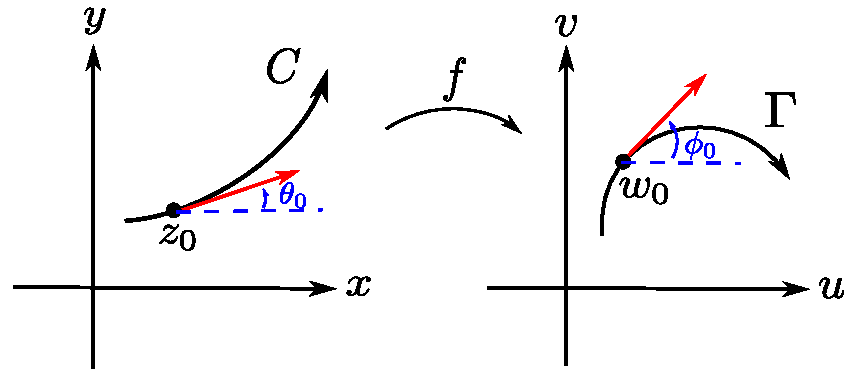
\includegraphics[scale = 0.75]{Figuras/MapeoConforme1.pdf}
    \caption{}
    \label{fig:Conforme1}
\end{figure}

En consecuencia, si $w = f(z)$ es analítica en un punto $z_0$ y $f'(z_0) \neq 0$, entonces la recta tangente a $C$ en $z_0$ es rotada en un ángulo
$$\arg f'(z(t_0))$$

por la transformación $w = f(z)$.

Supongamos, ahora, que $C_1$ y $C_2$ son dos curvas suaves que pasan por $z_0$ y con ángulos de inclinación $\theta_1$ y $\theta_2$ de las rectas tangentes, respectivamente. Entonces, por lo anterior, tenemos
\begin{align*}
    \phi_1 &= \theta_1 + \arg f'(z(t_0)) \\
    \phi_2 &= \theta_2 + \arg f'(z(t_0))
\end{align*}

y, por tanto,
$$\phi_2 - \phi_1 = \theta_2 - \theta_1,$$

es decir, el ángulo $\alpha = \phi_2 - \phi_1$ formado por $\Gamma_1$ a $\Gamma_2$ tiene igual magnitud y sentido que el ángulo $\alpha = \theta_2 - \theta_1$ formado por $C_1$ y $C_2$.

\begin{figure}[H]
    \centering
    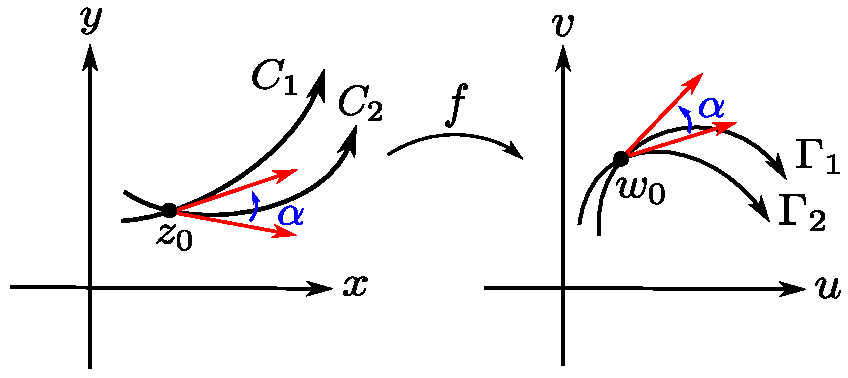
\includegraphics[scale = 0.75]{Figuras/MapeoConforme2.pdf}
    \caption{Preservación de la magnitud y el sentido del ángulo.}
    \label{fig:Conforme2}
\end{figure}

\begin{defi}
Una función que preserva magnitud y sentido de ángulos entre dos curvas suaves que pasan a través de un punto específico se dice una \textbf{aplicación conforme en tal punto}. Diremos que $f$ es, simplemente, una \textbf{aplicación conforme} si es conforme en cada punto.
\end{defi}

\begin{teorema}
Si $f$ es analítica y $f'(z) \neq 0$ para todo punto de su dominio, entonces $f$ es una aplicación conforme.
\end{teorema}

\begin{ejemplo}
Sea $D = \{z \in \mathbb{C}: Re(z) > 0, Im(z) > 0 \}$ y $F = \{z \in \mathbb{C}: Im(z) > 0\}$. La función $f: D \rightarrow F$, $f(z) = z^2$ es conformal en $D$, pues $f$ es analítica aquí y $f'(z) = 2z \neq 0$. En cambio $g: \mathbb{C} \rightarrow \mathbb{C}$, $g(z) = z^2$ no es conforme en $z_0 = 0$, ya que el ángulo que forman los ejes coordenados es $\pi/2$, en cambio, en sus imágenes forman un ángulo $\pi$. Justamente, $g'(0) = 0$.
\end{ejemplo}

\begin{propo}
Si $f$ es una transformación conforme, analítica en su dominio y biyectiva, entonces $f^{-1}$ es también conforme.
\end{propo}

\begin{proof}
La inversa es también analítica y
$$\left( f^{-1}\right)'(w) = \frac{1}{f'(z)} \neq 0,$$

donde $f(z) = w$.
\end{proof}

\begin{propo}
Si $f$ y $g$ son funciones analíticas tales que $g \circ f$ existe, $f'(z_0) \neq 0$ y $g'(f(z_0)) \neq 0$, entonces $g \circ f$ es conformal en $z_0$.
\end{propo}

\begin{proof}
Por la regla de la cadena, la compuesta $g \circ f$ es analítica y
$$(g\circ f) (z_0) = g'(f(z_0)) f'(z_0) \neq 0.$$

Probando así el teorema.

\end{proof}

Dado dos dominios $D$ y $E$, ¿será posible tener una aplicación conforme $f: D \rightarrow E$? La respuesta es positiva, pero la demostración requiere mayores resultados que se escapan del curso.

\begin{teorema}[de la aplicación de Riemann] \label{RiemannMap}
Sea $D$ una región simplemente conexa tal que $D \neq \mathbb{C}$. Entonces, existe una aplicación conforme biyectiva $f: D \rightarrow B$ donde $B = \{z \in \mathbb{C} : |z| < 1\}$. Más aún, para algún $z_0 \in D$ fijo, podemos encontrar una función $f$ tal que $f(z_0) = 0$ y $f'(z_0) > 0$. Con tal especificación, $f$ es única.
\end{teorema}

Asumiendo el teorema de la aplicación de Riemann, es posible dar respuesta a la pregunta mencionada arriba.

\begin{propo}
Sean $D$ y $E$ dos regiones simplemente conexas con $D \neq \mathbb{C}$ y $E \neq \mathbb{C}$, entonces existe una aplicación conforme biyectiva $g: D \rightarrow E$. 
\end{propo}

\begin{proof}
Por el teorema de la aplicación de Riemann, existen dos aplicaciones conformes biyectivas $f: D \rightarrow B$ y $h: E \rightarrow B$. Definiendo $g = h^{-1} \circ f$, se tiene la proposición.

\begin{figure}[H]
    \centering
    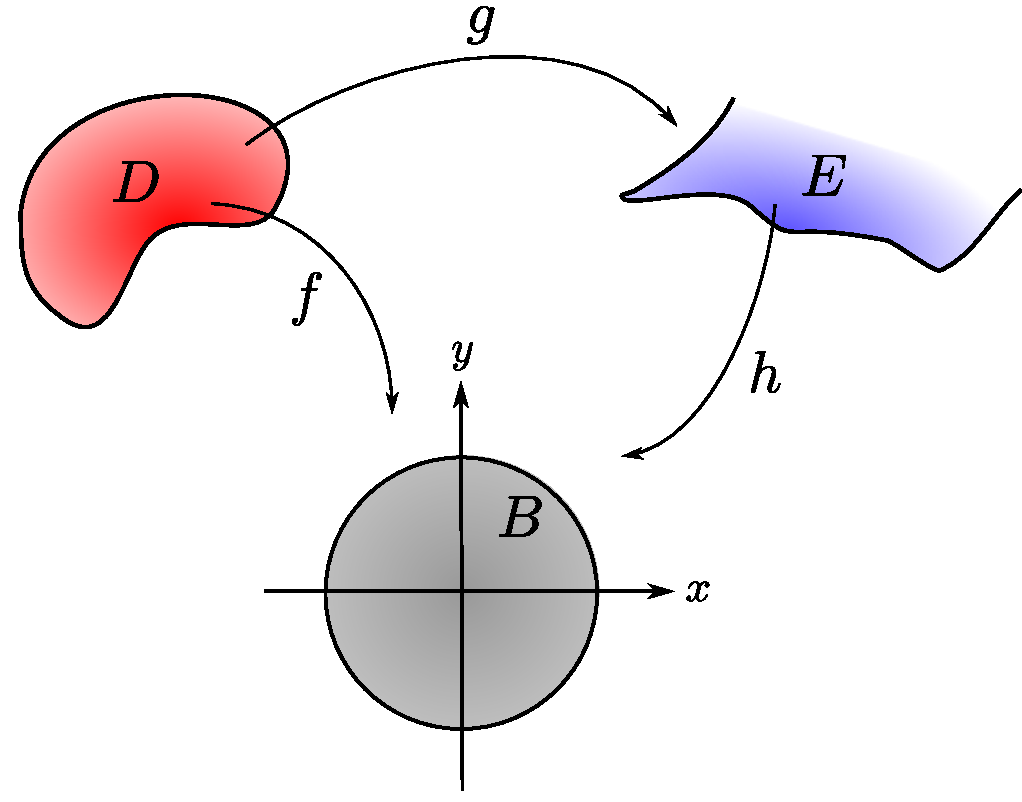
\includegraphics[scale = 0.5]{Figuras/MapeoConforme3.pdf}
    \caption{Aplicación entre dos regiones simplemente conexas.}
    \label{fig:Conforme3}
\end{figure}
\end{proof}

\begin{lema}[de Schwarz]
Sea $f(z)$ una función analítica en  $D = \{z \in \mathbb{C}: |z| < 1 \}$, y $f(0) = 0$, $|f(z)| \leq 1$. Entonces, 
\begin{equation}
 \forall z \in D:~ |f(z)| \leq |z|   \label{LemaSchawarz1}
\end{equation}

y
\begin{equation}
 |f'(0)| \leq 1. \label{LemaSchawarz2}
\end{equation}

La igualdad \eqref{LemaSchawarz1} ocurre en algún punto $0 \neq z \in D$ si y sólo si $f(z) =  \alpha z$, donde $\alpha \in \mathbb{C}$ tal que $|\alpha| = 1$.
\end{lema}
\begin{proof}

Sea 
$$g(z) = \left\{ \begin{array}{cl}
    \frac{f(z)}{z}, & \mbox{si}~ z\neq 0  \\
    f'(0), & \mbox{si}~ z = 0 
\end{array} \right. .$$

Probemos que $g$ es analítica en $D$. Como $f$ es analítica para  $|z| < 1$ y $f(0) = 0$, podemos escribir $f$ como la siguiente serie de potencias
$$f(z) = a_1z + a_2 z^2 + \cdots = \sum_{n=1}^{\infty} a_n z^n, \quad |z| < 1 $$

donde se hizo $a_0 = f(0) = 0$. Luego,
$$\frac{f(z)}{z} = a_1 + a_2 z + a_3 z^2 + \cdots = \sum_{n=0}^{\infty} a_{n+1} z^n.$$

Entonces, $z = 0$ es una singularidad removible de $f(z)/z$, así definiendo la función en $z = 0$ como $a_1 = f'(0)$, la función resultante es $g$, la cual es analítica en todo $D$. 

Sea $D_r = \{z \in \mathbb{C} : |z| \leq r\}$ para $0 <r <1$. Entonces, $g$ es analítica en $D_r$, y en $|z| = r$, se cumple que
$$|g(z)| = \left| \frac{f(z)}{z} \right| \leq \frac{1}{r}.$$

Por el teorema del módulo máximo,
$$\forall z \in D_r: ~ |g(z)| \leq \frac{1}{r} \Rightarrow |f(z)| \leq \frac{|z|}{r}.$$

Si mantenemos $z \in D$ fijo, podemos tomar  $r \to 1$ para sí obtener
$$|f(z)| \leq |z|.$$

Claramente, $|g(0)| \leq 1$, ésto es, $|f'(0)| \leq 1$.

Finalmente, si $|f(z_0)/z_0| = 1$ para algún $z_0 \neq 0$ en el disco unitario, entonces, por el teorema del módulo máximo, $f(z)/z$ no puede tener un máximo a menos que sea constante, así existe una constante $\alpha$ con $|\alpha| = 1$ tal que $f(z)/z = \alpha.$

\end{proof}

\subsection*{Prueba de la unicidad del teorema \ref{RiemannMap}*}

\begin{proof}
Supongamos que $f$ y $g$ son mapeos conformes biyectivos de $D$ sobre $B$, con $f(z_0) = g(z_0) = 0$, $f'(z_0) > 0$ y $g'(z_0) > 0$. Queremos mostrar que $f(z) = g(z)$ para todo $z \in D$. Para hacer ésto, definamos $h: B \rightarrow B$, $h(w) = g(f^{-1}(w))$, la cual es analítica en $B(0,1)$ y $h(0) = g(f^{-1}(0)) = g(z_0) = 0$. Por el lema de Schwarz, $|h(w)|\leq |w|$ para todo $w \in B$. Exactamente el mismo argumento se aplica a $h^{-1} = f \circ g^{-1}$, así que $|h^{-1}(\xi)| \leq |\xi|$ para todo $\xi \in D$. Con $\xi = h(w)$ esto da $|w| \leq h(w)$. Al combinar estas desigualdades, obtenemos $|h(w)| = w$ para todo $w\in B$. El lema de Schwarz nos dice ahora que $h(w) = \alpha w$ para un $\alpha \in \mathbb{C}$, con $|\alpha| = 1$. Así, $\alpha w = g(f^{-1}(w))$. Con $z = f^{-1}(w)$ obtenemos $\alpha f(z) = g(z)$ para todo $z\in D$. En particular, $\alpha f'(z_0) = g'(z_0)$. Ya que tanto $f'(z_0)$ como $g'(z_0)$ son números reales positivos, también lo es $\alpha$. Así, $\alpha = 1$ y, por tanto, $f(z) = g(z)$, como se quería.
\end{proof}

\section{Transformaciones de Möbius}

Un ejemplo importante de aplicaciones conformes son las \textbf{transformaciones fraccionales lineales} o \textbf{de Möbius}:
$$T(z) = \frac{az+b}{cz+d}, \quad z \neq - \frac{d}{c},$$

con $ad-bc \neq 0$. En efecto,
$$T\,'(z) = \frac{ad-bc}{(cz+d)^2} \neq 0.$$

Luego, $T$ es una aplicación conforme en cada $z\in \mathbb{C} \setminus \left\{-\frac{d}{c} \right\}$.

Son biyectivas en $\mathbb{C}\setminus \left\{-\frac{d}{c} \right\}$ sobre $\mathbb{C}\setminus \left\{\frac{a}{c} \right\}$ y, por tanto, su inversa
$$T^{-1}(w) = \frac{(-d)w + b}{cw-a}$$

es también conforme.

Notar que $T = T_4 \circ T_3 \circ T_2 \circ T_1$, donde 
\begin{align*}
    T_1(z) &= z + \frac{d}{c}; \quad T_2(z) = \frac{1}{z}; \\
    T_3(z) &= \frac{bc-ad}{c^2}z; \quad  T_4(z) = z+ \frac{a}{c}.
\end{align*}

\begin{ejemplo}
Dada la transformación de Möbius
$$T(z) = \frac{az+b}{cz+d}.$$

Si $a = 1$, $c = 0$ y $d = 1$, obtenemos $T(z) = z+b$, la cual es una traslación de los puntos en el plano complejo de acuerdo al vector $b$.

Si $b = c = 0$ y $d = 1$, obtenemos $T(z) = az$, la cual es una rotación por $\arg(a)$ y una amplificación por $|a|$.

Finalmente, si $a = d = 0$ y $b = c = 1$, obtenemos $T(z) = 1/z$, la cual es una inversión donde envía a todo $z = r e^{i\theta}$ a $z^{-1} = \overline{z}/|z|^2 = r^{-1}  e^{-i\theta}$.
\end{ejemplo}

\textbf{Observaciones:}

\begin{enumerate}
    \item La composición de dos transformaciones de Möbius es una transformación de Möbius (ejercicio para el lector).
    
    \item Sea
    $$T(z) = \frac{az+b}{cz+d}; \quad z \neq - \frac{d}{c}$$
    
    una transformación de Möbius. Notar que
    $$\frac{(\lambda a) z + \lambda b}{(\lambda c)z + \lambda d} = \frac{az + b}{cz+d},$$
    
    es decir, los coeficientes $a, b, c, d$ no son únicos.
    
    \item Por otro lado, podemos extender una transformación de Möbius al plano extendido $\overline{\mathbb{C}}$ como sigue:
    $$T(z) = \left\{ \begin{array}{cl}
        \frac{az+b}{cz+d}, & \mbox{si}~ z \neq - \frac{d}{c}, \infty  \\
        \frac{a}{c}, &  \mbox{si}~ z = \infty \\
        \infty, & \mbox{si}~ z = - \frac{d}{c}
    \end{array} \right. .$$
\end{enumerate}    

\begin{propo}
Cualquier mapeo conforme de $D = \{z \in \mathbb{C}: |z| < 1\}$ sobre si mismo es una transformación fraccional lineal de la forma
$$T(z) = e^{i\theta} \frac{z-z_0}{1-\overline{z_0} z}$$

para algún $z_0 \in D$ fijo y $\theta \in [0,2\pi[$; más aún, cualquier $T$ de esta forma es un mapeo conforme de $D$ sobre $D$.
\end{propo}

\begin{proof}
Primero verifiquemos que para $T$ de esta forma, $|z| = 1$ implica que $|T(z)| = 1$. En efecto,
$$|T(z)| = \left|\frac{z-z_0}{1-\overline{z_0} z} \right| = \frac{|z-z_0|}{|z| \,|z^{-1} - \overline{z_0}|}.$$

Pero $|z| = 1$ y, por tanto, $z^{-1} = \overline{z}$. Así, obtenemos
$$|T(z)|= \frac{|z-z_0|}{|\overline{z} - \overline{z_0}|} = \frac{|z-z_0|}{|\,\overline{z-z_0}\,|} = 1.$$

La única singularidad de $T$ está en $z = \overline{z_0}^{-1}$, que está fuera del círculo unitario, pues
$$|z| = \left|\frac{z_0}{z_0 \overline{z_0}} \right| = \frac{|z_0|}{|z_0|^2} = \frac{1}{|z_0|} \geq 1.$$

Entonces, por el teorema del módulo máximo, $|T(z)| \leq 1$ para todo $z \in D$, es decir, $T$ transforma $D$ en $D$ (no sobre a priori). Pero su inversa,
$$T^{-1}(w) = e^{-i\theta} \left[\frac{w - (-e^{i\theta}z_0)}{1-(-e^{-i\theta} \overline{z_0})w} \right],$$

la cual, puesto que tiene la misma forma que $T$, es también un mapeo de $D$ en $D$. Así que $T$ es conforme de $D$ sobre $D$.

Sea $R: D \rightarrow D$ cualquier mapeo conforme. Sea $z_0 = R^{-1}(0)$ y sea $\theta = \arg R'(z_0)$. El mapeo $T$ definido, también tiene $T(z_0) = 0$ y  $\theta = \arg T'(z_0)$. En efecto,
$$T\,'(z) = e^{i\theta} \left[ \frac{1-|z_0|^{2}}{(1-\overline{z_0} z)^2} \right]$$

el cual, en $z = z_0$, es igual a
$$e^{i\theta} \left(\frac{1}{1-|z_0|^2} \right)$$

una constante real por $e^{i\theta}$. Así, por la unicidad de los mapeos conformes, $R = T$.
\end{proof}

Este resultado nos dice que la única forma de transformar un disco sobre sí mismo conformemente, es por medio de una transformación fraccional lineal. Estas transformaciones poseen otras propiedades adicionales, como se mostrará en los siguientes resultados.

\begin{propo}
Sea $T$ una transformación fraccional lineal. Si $L \subset \mathbb{C}$ es una línea recta y $S \subset \mathbb{C}$ es una circunferencia, entonces $T(L)$ es una línea recta o una circunferencia, y $T(S)$ es una línea recta o una circunferencia.
\end{propo}

\begin{proof}
Escribamos $T = T_4 \circ T_3 \circ T_2 \circ T_1$, donde 
\begin{align*}
    T_1(z) &= z + \frac{d}{c}; \quad T_2(z) = \frac{1}{z}; \\
    T_3(z) &= \frac{bc-ad}{c^2}z; \quad T_4(z) = z+ \frac{a}{c}.
\end{align*}

Es claro que $T_1$, $T_3$ y $T_4$ transforman líneas en líneas, y circunferencias en circunferencias. Así que si podemos verificar la conclusión para $T(z) = 1/z$, la demostración estará completa. Asumamos primero que $S: |z-z_0| = r$ y sea
$$f(S) = \left\{ w = \frac{1}{z} : z \in S\right\}.$$

Escribamos $S$ de la forma
$$(z-z_0)(\overline{z} - \overline{z_0}) = r^2,$$

tenemos
$$z \overline{z} - z_0 \overline{z} - \overline{z_0} z = r^2 - |z_0|^2$$

o, en términos de $w$,
\begin{equation}
\frac{1}{w \overline{w}} - \frac{z_0}{\overline{w}} - \frac{\overline{z_0}}{w} = r^2-|z_0|^2.    \label{Mobius1}
\end{equation}

Si $r = |z_0|$, es decir, si $S$ pasa a través del origen, \eqref{Mobius1} es equivalente a 
$$1- z_0 w - \overline{z_0} \overline{w} = 0 \Rightarrow Re(z_0 w) = \frac{1}{2}.$$

En ese caso, si $z_0 = x_0 + iy_0$ y $w = u+iv$, la ecuación se convierte en
$$ux_0 - vy_0 = \frac{1}{2},$$

ésto es, $f(S)$ es una línea en el plano $uv$.

Por otro lado, si $r \neq |z_0|$, entonces \eqref{Mobius1} es equivalente a
$$w \overline{w} - \left( \frac{\overline{z_0}}{|\overline{z_0}|^2 -r^2} \right) \overline{w} - \left( \frac{z_0}{|\overline{z_0}|^2 -r^2} \right) w = - \frac{1}{|z_0|^2 -r^2},$$

definiendo $\beta = \overline{z_0}/(|\overline{z_0}|^2 -r^2)$, obtenemos
$$w \overline{w} - \beta \overline{w} - \overline{\beta} w + |\beta|^2 = \frac{r^2}{(|z_0|^{2} - r^2)^2}.$$

Por lo tanto,
$$|w - \beta|^2 = \left(\frac{r}{|z_0|^{2} - r^2} \right)^2,$$

es decir, $f(S)$ es una circunferencia con centro $\beta$ y radio $|r/(|z_0|^2-r^2)|$.

Finalmente, para la línea recta $L$, tenemos que si $z = x+iy \in L$, entonces existen $a,b,c \in \mathbb{R}$, no todos nulos, tales que
$$ax+by = c.$$

Haciendo $z_0 = a-bi$, 
$$Re(z_0 z) = c \Rightarrow z_0 z + \overline{z_0} \overline{z} = 2c.$$

Se sigue, como lo desarrollado previamente, que $f(L)$ es o una circunferencia o una línea.

 \end{proof}

\begin{propo}
Si $z_1, z_2, z_3, w_1, w_2, w_3 \in \mathbb{C}$ tales que $z_i \neq z_j$ y $w_i \neq w_j$ para $i \neq j$, entonces existe una única transformación de Möbius que lleva $z_i \to w_i$
\end{propo}

\begin{proof}
Para $z,w \in \mathbb{C}$, se define la ecuación
\begin{equation}
 \frac{w-w_1}{w-w_2} \frac{w_3-w_2}{w_3-w_1} = \frac{z-z_1}{z-z_2} \frac{z_3 - z_2}{z_3 - z_1}.  \label{Mobius1} 
\end{equation}

donde su solución $w = T(z)$  es una transformación de Möbius. En efecto, notemos que cada lado de la ecuación \eqref{Mobius1} es una transformación de Möbius, entonces si definimos
$$R(w) =  \frac{w-w_1}{w-w_2} \frac{w_3-w_2}{w_3-w_1}, \quad S(z) = \frac{z-z_1}{z-z_2} \frac{z_3 - z_2}{z_3 - z_1},$$

dos transformaciones de Möbius, tenemos que son invertibles. Luego,
$$R(w) = S(z) \Rightarrow w = R^{-1}(S(z)) = T(z),$$

donde $T = R^{-1} \circ S$.

Además, $T(z_i) = w_i$. Por tanto, nos queda por demostrar que es única. Para ello, utilizaremos la definición de la transformación de Möbius $S(z)$, la cual manda $z_1$ a 0, $z_3$ a 1, y $z_2$ a $\infty$ ($z_2$ es la singularidad de $S$). Sea $F$ cualquier otra transformación de Möbius,
$$F(z) = \frac{az + b}{cz + d}$$

con $R(z_1) = 0$, $R(z_3) = 1$ y $R(z_2) = \infty$ (ésto es, $c z_2 + d = 0$). Entonces, $az_1 + b = 0$, $c z_2 + d = 0$ y $(az_3 + b)/(cz_3+d) = 1$. De este modo, obtenemos que $a = -b/z_1$ y $c = -d/z_2$, así que la última condición da $b(z_1-z_3)/z_1 = d(z_2-z_3)/z_2$. Al sustituir en $F$, vemos que $F = S$.

Usemos este resultado para probar que $T$ es única. Sea $T$ cualquier transformación de Möbius que manda $z_i$ a $w_i$, $i = 1,2,3$. La transformación de Möbius $S\circ T^{-1}$ manda $w_1 = T(z_1)$ a 0, $w_3 = T(z_3)$ a 1, y $w_2 = T(z_2)$ a $\infty$. Por lo tanto, $ST^{-1}$ está determinado de esta manera única, por los cálculos precedentes. Así, $T$ está determinada de manera única, ya que $T = (S \circ T^{-1})^{-1} \circ S.$

\end{proof}

Se sigue que podemos usar una transformación de Möbius para mapear cualesquiera tres puntos en otros tres. Tres puntos están en una única circunferencia o línea, la transformación manda la circunferencia (o línea) a través de $z_1, z_2,z_3$, en la circunferencia (o línea) que pasa por $w_1, w_2, w_3$. El interior del disco se mapea a uno o dos semi-planos. Para determinar cuales, uno puede verificar donde el centro se mapea (o cualquier otro punto).

\newpage
\textbf{Observación:} Un \textbf{punto fijo} de una transformación $T$ es un $z_0$ tal que $T(z_0) = z_0$. Una transformación de Möbius distinta de la identidad tiene, a lo más, dos puntos fijos. En efecto,
    $$T(z) = z \Rightarrow \frac{az+b}{cz+d} = z \Rightarrow cz^2 + (d-a) z - b = 0.$$
    
    Notar que si $T$ tiene más de tres puntos fijos, entonces $T = Id$. Para probar ésto, usar
    $$\frac{w-w_1}{w-w_2} \frac{w_3-w_2}{w_3-w_1} = \frac{z-z_1}{z-z_2} \frac{z_3 - z_2}{z_3 - z_1}.$$

\section{Ejemplos de mapeos conformes}

Algunas transformaciones más comunes están representadas en las figuras \ref{fig:EjMapeosConformes1}, \ref{fig:EjMapeosConformes2} y \ref{fig:EjMapeosConformes3}.

\begin{ejemplo}
Encuentre un mapeo conforme que lleve al conjunto
$$A = \{z \in \mathbb{C} : 0 < \arg(z) < \pi/2, 0 < |z| < 1 \}$$

al conjunto
$$D = \{ z \in \mathbb{C} : |z| < 1\}.$$

\textbf{Solución:} En un principio uno está tentado a efectuar la transformación $z \mapsto z^4$ de tal forma que se complete el disco, sin embargo, esta transformación no mapea $A$ sobre $D$, pues omite el semieje real positivo.

Primero, consideremos $z \mapsto z^2$. Ésto mapea $A$ sobre $B = \{z \in \mathbb{C}: 0 < \arg(z) < \pi, 0 < |z| < 1\}$. Consultando a la figura \ref{fig:EjMapeosConformes1} (iv), mapeamos $B$ al primer cuadrante por $z \mapsto (1+z)/(1-z)$ y al elevar al cuadrado de nuevo, obtenemos el semiplano superior. Finalmente, usamos la transformación $z \mapsto (z-i)/(z+i)$ para así llegar al disco abierto unitario $D$.

\begin{figure}[H]
    \centering
    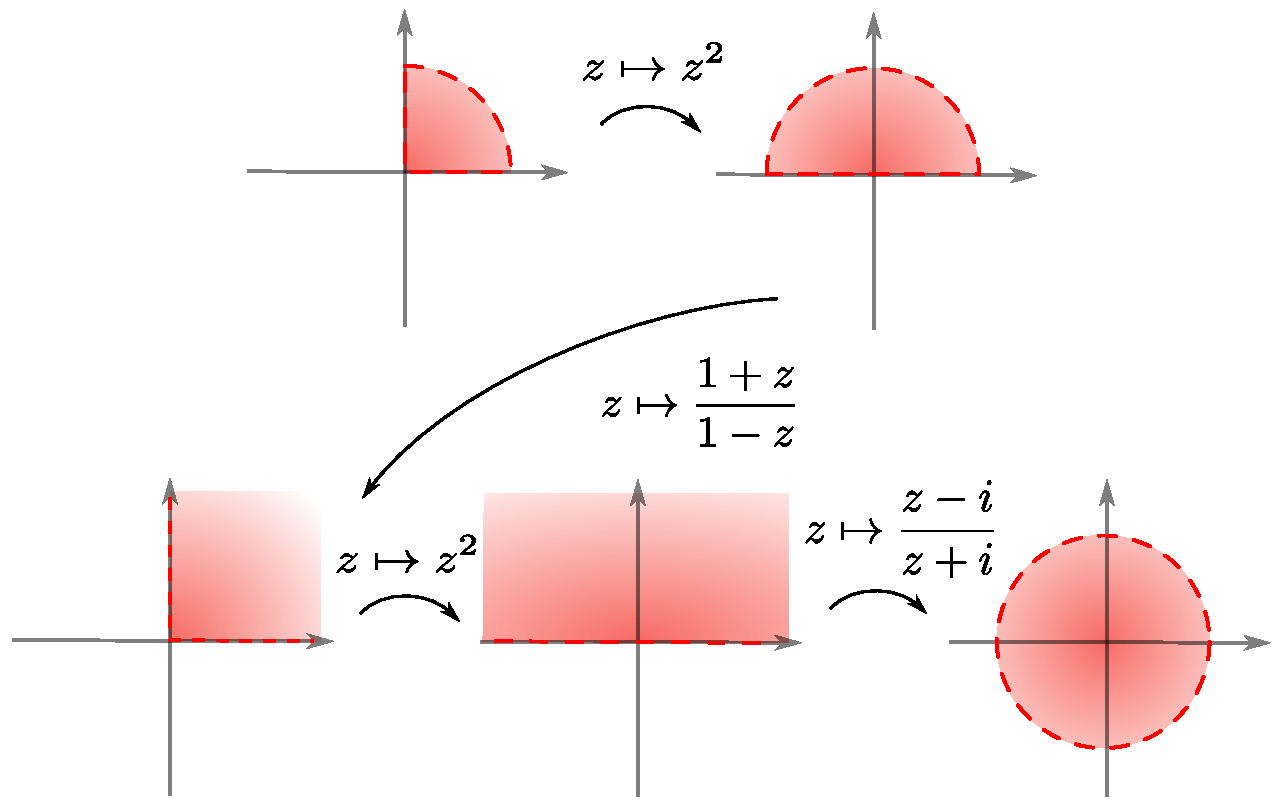
\includegraphics[scale = 0.6]{Figuras/MapeoConforme7.pdf}
    \caption{Sucesión de transformaciones que manda al cuarto de disco abierto al disco completo.}
    \label{fig:EjMapConformal}
\end{figure}

Por lo tanto, obtenemos nuestro mapeo conforme al hacer la sucesiva sustitución:
\begin{align*}
    w_1 &= z^2, \\
    w_2 &= \frac{1 + w_1}{1-w_1} = \frac{1+z^2}{1-z^2}, \\
    w_3 &= w_2^2 = \left( \frac{1+z^2}{1-z^2}\right)^2, \\
    w_4 &= \frac{w_3-i}{w_3 + i} = \frac{\left( \frac{1+z^2}{1-z^2}\right)^2 - i}{\left( \frac{1+z^2}{1-z^2}\right)^2+i}.
\end{align*}

Entonces,
$$f(z) = \frac{(1+z^2)^2 - i (1-z^2)^2}{(1+z^2)^2 + i (1-z^2)^2}.$$
\end{ejemplo}

\begin{ejemplo}
Estudie la acción de la función
$$f(z) = \frac{z-1}{z-3}$$

en la circunferencia unitaria $C$, el disco unitario $B$ y el eje real.
\\

\textbf{Solución:} Primero evaluemos $f$ en los puntos de la circunferencia $1$, $i$ y $-1$:
$$f(1) = 0, ~ f(i) = \frac{2}{5}-\frac{1}{5}i, ~ f(-1) = \frac{1}{2}.$$

Claramente las imágenes de $f$ no pertenece a una recta, por lo tanto la transformación de Möbius mapea la circunferencia unitaria en la circunferencia que pasa por $0$, $\frac{2}{5}-\frac{1}{5}i$ y $\frac{1}{2}$. 

Ahora, si evaluamos $f$ en un punto del disco unitario, como $z = 0$, $f(0) = 1/3$, la cual está en el interior de la circunferencia imagen. Entonces, $f$ mapea el disco unitario a otro disco cuya frontera es la circunferencia imagen.

Claramente $f$ manda al eje real sobre el eje real, pues la recta que pasa por $-1$, $0$ y $1$, va a la recta que pasa por $1/2$, $1/3$ y $0$. Ésto nos permitirá saber con precisión la circunferencia imagen. Aunque con los tres puntos podemos saber con precisión la ecuación de la circunferencia \footnote{La ecuación general de una circunferencia es $x^2 + y^2 + Ax + By + C = 0$ con $A,B,C \in \mathbb{R}$ no todos nulos}, usaremos el hecho de que $f$ es una transformación conforme. La curva $C$ cruza el eje real en ángulo recto en $\pm 1$ y, por ende, $f(C)$ debe cruzar el eje real también en ángulo recto, en $0$ y $1/2$. Entonces, $f(C)$ es la circunferencia de radio $1/4$ con centro $1/4$.
\end{ejemplo}

\newpage

\begin{figure}[H]
    \centering
    \includegraphics[scale = 0.7]{Figuras/MapeoConforme4.pdf}
    \caption{Transformaciones comunes parte 1.}
    \label{fig:EjMapeosConformes1}
\end{figure}

\begin{figure}[H]
    \centering
    \includegraphics[scale = 0.7]{Figuras/MapeoConforme5.pdf}
    \caption{Transformaciones comunes parte 2.}
    \label{fig:EjMapeosConformes2}
\end{figure}

\begin{figure}[H]
    \centering
    \includegraphics[scale = 0.7]{Figuras/MapeoConforme6.pdf}
    \caption{Transformaciones comunes parte 3.}
    \label{fig:EjMapeosConformes3}
\end{figure}

%\section{Aplicaciones Físicas}\subsection{Problema de Dirichlet y Neumann}\subsection{Conducción de calor}\subsection{Electrostática}\subsection{Hidrodinámica}






\begin{thebibliography}{99}

\bibitem{Agarwal} Agarwal, R. P., Perera, K. y Pinelas, S. (2011). \textit{An Introduction to Complex Analysis}. Springer New York. 

\bibitem{Aguayo} Aguayo, J. (2020). \textit{Apuntes del curso Cálculo IV}. Universidad de Concepción.

\bibitem{Apostol} Apostol, T. M. (1999). \textit{Calculus volumen I} (2da edición). Barcelona, España: Editorial Reverté, S. A.

\bibitem{Asmar} Asmar, N. H y Grafakos, L. (2018). \textit{Complex Analysis with Applications}. Springer Cham. 

\bibitem{Churchill} Churchill, R. V. y Brown J. W. (1992). \textit{Variable compleja y aplicaciones} (5ta edición). Madrid, España: McGraw-Hill.

\bibitem{Marsden} Marsden, J.E. y Hoffman, M.J. (1996). \textit{Análisis básico de variable compleja}. México: Editorial Trillas. 

\end{thebibliography}

\end{document}